%%%%%%%%%%%%%%%%%%%%%%%%%%%%%%%%%%%%%%%%%
% Short Sectioned Assignment LaTeX Template Version 1.0 (5/5/12)
% This template has been downloaded from: http://www.LaTeXTemplates.com
% Original author:  Frits Wenneker (http://www.howtotex.com)
% License: CC BY-NC-SA 3.0 (http://creativecommons.org/licenses/by-nc-sa/3.0/)
%%%%%%%%%%%%%%%%%%%%%%%%%%%%%%%%%%%%%%%%%

% \documentclass[paper=a4, fontsize=11pt]{scrartcl} % A4 paper and 11pt font size
\documentclass[11pt, a4paper]{book}
\usepackage[T1]{fontenc} % Use 8-bit encoding that has 256 glyphs
\usepackage[utf8]{inputenc}
%\usepackage{mathptmx} % Use the Adobe Utopia font for the document - comment this line to return to the LaTeX default
\usepackage{listings} % para insertar código con formato similar al editor
\usepackage{color}  % si quieres usar colores en tu código
\usepackage[spanish, es-tabla]{babel} % Selecciona el español para palabras introducidas automáticamente, p.ej. "septiembre" en la fecha y especifica que se use la palabra Tabla en vez de Cuadro
\usepackage{url} % ,href} %para incluir URLs e hipervínculos dentro del texto (aunque hay que instalar href)
\usepackage{graphics,graphicx, float} %para incluir imágenes y colocarlas
\usepackage[gen]{eurosym} %para incluir el símbolo del euro
\usepackage{cite} %para incluir citas del archivo <nombre>.bib
\usepackage{enumerate}
\usepackage{enumitem}
\usepackage{hyperref}
\usepackage{graphicx}
\usepackage{tabularx}
\usepackage{booktabs}
\usepackage{textcomp}
\usepackage{adjustbox}
\usepackage{geometry}
\usepackage{amsmath}
\usepackage{amsthm} % Añadir este paquete
\usepackage{amsfonts}
\usepackage{amssymb}
\usepackage{subfigure}
\usepackage{textcomp}
\usepackage{longtable}
\usepackage{mwe} % Paquete necesario para la columna tipo 'm'
\usepackage{mathrsfs}
\usepackage{upquote}
\usepackage{mdframed}


\lstdefinestyle{lamportStyle}{
    language=Pascal,          % Usar configuración base de Pascal
    basicstyle=\ttfamily\small,
    numbers=left,
    numberstyle=\tiny,
    stepnumber=1,
    numbersep=5pt,
    tabsize=4,
    extendedchars=true,
    breaklines=true,
    keywordstyle=\color{blue},
    stringstyle=\color{orange}, % Cadena de caracteres en naranja
    commentstyle=\color{gray},
    frame=b,
    morekeywords={program, procedure, function, process, integer, real, char, boolean, string, begin, end, cobegin, coend, return},
    captionpos=b             % Posiciona el caption debajo del bloque de código   
}


\lstnewenvironment{BNFCode}{%
\lstset{
  language={}, % Vacío, no basarse en ningún lenguaje específico
  basicstyle=\ttfamily\color{black}, % Fuente de estilo básico en color negro
  morestring=[b]", % Define las cadenas de texto entre comillas dobles
  stringstyle=\color{red}, % Color rojo para cadenas de texto
  commentstyle=\color{orange}, % Color naranja para comentarios
  morecomment=[l]{\#}, % Define cómo se indican los comentarios
  keepspaces=true, % Mantiene los espacios
  breaklines=true, % Permite romper las líneas
  breakindent=1.5cm, % Sangría después de romper una línea
  breakatwhitespace=false, % Permite romper en cualquier espacio, no solo en espacios en blanco
  columns=fullflexible,
}
}{}

\lstdefinestyle{customflex}{
    language=C, % Flex se basa en C, así que esto debería resaltar la mayoría de la sintaxis correctamente
    basicstyle=\ttfamily\small,
    commentstyle=\color{gray},
    keywordstyle=\color{blue},
    numbers=left,
    breaklines=true,
    frame=single,
    captionpos=b
    \lstset{upquote=true}
}

\lstdefinestyle{myInlineCode}{
    basicstyle=\ttfamily,
    breaklines=true,  % Opcional: permite que el código se divida entre líneas
    keepspaces=true   % Opcional: conserva los espacios en el código
}


\usepackage[table,xcdraw]{xcolor}
\hypersetup{
	colorlinks=true,	% false: boxed links; true: colored links
	linkcolor=black,	% color of internal links
	urlcolor=cyan		% color of external links
}
%\renewcommand{\familydefault}{\sfdefault}
\usepackage{fancyhdr} % Custom headers and footers
\pagestyle{fancyplain} % Makes all pages in the document conform to the custom headers and footers
\fancyhead[L]{} % Empty left header
\fancyhead[C]{} % Empty center header
\fancyhead[R]{Daniel Pérez Ruiz} % My name
\fancyfoot[L]{} % Empty left footer
\fancyfoot[C]{} % Empty center footer
\fancyfoot[R]{\thepage} % Page numbering for right footer
%\renewcommand{\headrulewidth}{0pt} % Remove header underlines
\renewcommand{\footrulewidth}{0pt} % Remove footer underlines
\setlength{\headheight}{13.6pt} % Customize the height of the header

\usepackage{titlesec, blindtext, color}
\definecolor{gray75}{gray}{0.75}
\newcommand{\hsp}{\hspace{20pt}}
\titleformat{\chapter}[hang]{\Huge\bfseries}{\thechapter\hsp\textcolor{gray75}{|}\hsp}{0pt}{\Huge\bfseries}
\setcounter{secnumdepth}{4}
\usepackage[Lenny]{fncychap}


\newcolumntype{M}[1]{>{\centering\arraybackslash}m{#1}}

\renewcommand{\lstlistingname}{Programa}
\newcommand{\code}[1]{\lstinline[style=myInlineCode]!#1!}

\newtheorem{teorema}{Teorema}[section]
\newtheorem{definicion}[teorema]{Definición}
\newtheorem{corolario}[teorema]{Corolario}
\newtheorem{proposicion}[teorema]{Proposición}
\newtheorem{observacion}[teorema]{Observación}


\begin{document}

	% Plantilla portada UGR
	\begin{titlepage}
\newlength{\centeroffset}
\setlength{\centeroffset}{-0.5\oddsidemargin}
\addtolength{\centeroffset}{0.5\evensidemargin}
\thispagestyle{empty}

\noindent\hspace*{\centeroffset}\begin{minipage}{\textwidth}

\centering

\includegraphics[width=0.9\textwidth]{logos/logo_ugr.jpg}\\[1.4cm]

\textsc{ \Large TRABAJO FIN DE GRADO\\[0.2cm]}
\small \textsc{DOBLE GRADO EN INGENIERÍA INFORMÁTICA Y MATEMÁTICAS}\\[1cm]

{\Huge\bfseries Simulador de Sistemas Concurrentes y Distribuidos \\}
\noindent\rule[-1ex]{\textwidth}{3pt}\\[3.5ex]
\end{minipage}

\vspace{1.5cm}
\noindent\hspace*{\centeroffset}
\begin{minipage}{\textwidth}
\centering

\textbf{Autor}\\ {Daniel Pérez Ruiz}\\[2.5ex]
\textbf{Director}\\ {Carlos Ureña Almagro}\\[1.2cm]

\begin{figure}[H]
  \centering
  
\includegraphics[width=.3\textwidth]{logos/etsiit_logo.png}\hspace{0.2\textwidth}
  
\includegraphics[width=.2\textwidth]{logos/ciencias-logo.png}
\end{figure}
%
\includegraphics[width=0.3\textwidth]{logos/etsiit_logo.png}\\[0.1cm]
\textsc{Escuela Técnica Superior de Ingenierías Informática y de Telecomunicación}\\[0.1cm]
\textsc{Y}\\
\textsc{Facultad de Ciencias}\\
\textsc{---}\\
Granada, Junio de 2023
\end{minipage}
\end{titlepage}


	% Plantilla prefacio UGR
	\thispagestyle{empty}

\begin{center}
{\large\bfseries Simulador de Sistemas Concurrentes y Distribuidos. Lógica Temporal de Acciones }\\
\end{center}
\begin{center}
Daniel Pérez Ruiz\\
\end{center}

%\vspace{0.7cm}

\vspace{0.5cm}
\noindent\textbf{Palabras clave}: \textit{ágil, concurrencia, sistema, programa, lógica, instrucción, lenguaje, compilador, máquina virtual}
\vspace{0.7cm}

\noindent\textbf{Resumen}\\
Este trabajo se centra en el desarrollo de un compilador para un lenguaje de programación, nombrado Lamport en honor a Leslie Lamport y su influencia en el ámbito de los sistemas concurrentes y distribuidos, especialmente a través de su contribución con la Lógica Temporal de Acciones (TLA). Además este proyecto presenta un estudio detallado de TLA y un ejemplo práctico de su aplicación en la especificación de sistemas, proporcionando una perspectiva matemática y formal para la especificación y verificación de sistemas concurrentes en general. El objetivo principal, sin embargo, es la creación de una herramienta práctica que concretice los conceptos de concurrencia en una aplicación tangible y accesible para los usuarios.

El compilador de Lamport ha sido diseñado específicamente para simular sistemas concurrentes y distribuidos, permitiendo así a los usuarios interactuar directamente con las complejidades y retos inherentes a la programación en este campo. Desarrollado bajo una metodología ágil y utilizando las capacidades de los lenguajes C y C++, el compilador profundiza en la comprensión de aspectos clave como la sincronización de procesos o el manejo de bloqueos, a parte de ser un lenguaje totalmente funcional para programas secuenciales.

El trabajo también incluye una exploración de los principios fundamentales de los sistemas concurrentes y distribuidos, proporcionando el marco teórico esencial para comprender y utilizar eficazmente el compilador Lamport. Se examinan posibles ampliaciones y mejoras del compilador, incluyendo su eventual evolución hacia un modelo de Software as a Service (SaaS), la incorporación de mecanismos de sincronización más sofisticados y la expansión de la gramática del lenguaje.

\cleardoublepage

\begin{center}
	{\large\bfseries Concurrent and Distributed Systems Simulator. Temporal Logic of Actions}\\
\end{center}
\begin{center}
	Daniel Pérez Ruiz\\
\end{center}
\vspace{0.5cm}
\noindent\textbf{Keywords}: \textit{agile, concurrency, system, program, logic, instruction, language, compiler, virtual machine}
\vspace{0.7cm}

\noindent\textbf{Abstract}\\
This work focuses on the development of an compiler for a programming language, named Lamport in honor of Leslie Lamport and his influence in the field of concurrent and distributed systems, particularly through his contribution to Temporal Logic of Actions (TLA). Additionally, this project presents a detailed study of TLA and a practical example of its application in system specification, offering a mathematical and formal perspective for the specification and verification of concurrent systems in general. The main goal, however, is to create a practical tool that materializes the concepts of concurrency into a tangible and accessible application for users.

The Lamport compiler has been specifically designed to simulate concurrent and distributed systems, thus allowing users to directly interact with the complexities and challenges inherent in programming in this field. Developed under an agile methodology and utilizing the capabilities of C and C++ languages, the compiler deepens the understanding of key aspects such as process synchronization or deadlock handling, apart from being a fully functional language for sequential programs.

The work also includes an exploration of the fundamental principles of concurrent and distributed systems, providing the essential theoretical framework to effectively understand and use the Lamport compiler. Potential extensions and improvements of the compiler are examined, including its eventual evolution into a Software as a Service (SaaS) model, the incorporation of more sophisticated synchronization mechanisms, and the expansion of the language grammar.



\cleardoublepage

\thispagestyle{empty}

\noindent\rule[-1ex]{\textwidth}{2pt}\\[4.5ex]

D. \textbf{Tutora/e(s)}, Profesor(a) del ...

\vspace{0.5cm}

\textbf{Informo:}

\vspace{0.5cm}

Que el presente trabajo, titulado \textit{\textbf{Simulador de Sistemas Concurrentes y Distribuidos. Lógica Temporal de Acciones}},
ha sido realizado bajo mi supervisión por \textbf{Daniel Pérez Ruiz}, y autorizo la defensa de dicho trabajo ante el tribunal
que corresponda.

\vspace{0.5cm}

Y para que conste, expiden y firman el presente informe en Granada a Noviembre de 2023.

\vspace{1cm}

\textbf{El/la director(a)/es: }

\vspace{5cm}

\noindent \textbf{(nombre completo tutor/a/es)}

\chapter*{Agradecimientos}

Desde que era muy pequeño mi madre siempre me ha dicho que, si ves una mariposa blanca, eso es señal de suerte. Aunque no me caracterizo por ser una persona supersticiosa, siempre he convivido con esa inocencia cada vez que tenía ante mis ojos una de ellas, aleteando, al son de la libertad, iluminando en mí una sonrisa.

\vspace{0.2cm}

A lo largo de mi vida he tenido muchas ocasiones donde sentía que me habían abandonado. Y la realidad, es que siempre me han acompañado, aunque muchas veces no las viera. Ahí se encontraban, danzando al compás de todas las melodías y letras, de todas aquellas canciones que en tiempos pasados resonaron en mi cabeza.

\vspace{0.2cm} 

A mi madre, a mi hermana Irene, a mi padre. A mis amigos de toda una vida Adrián, Alberto, Elías, Juanmi, Juan, Rafa Aguilar y Rafa Barrales. A mis amigos de esta nueva vida Lucía, Martín, Mery, Jaime, Jose, Joseja y Pablo. No hay suficientes palabras en este mundo para describir lo inmensos que son. A mi amiga Candela, por haber por fin coincidido en este camino tras muchas historias y canciones, y que prometo recorrerlo bailando una vez más. A mi amiga Elena, por haber sido la mayor voz que me guió y me dio luz cuando no la había. A Coral, por haber venido casi al final con su deslumbrante forma de ser, brindándome un nuevo y prometedor comienzo. A mis dos grandes mentores: mi tutor, Carlos, por ser mi fuente de inspiración desde que coincidí con él; y JJ, la persona que me enseñó a cómo encontrarme si me perdía en el camino.

\vspace{0.2cm}
En este trabajo dejo atrás una muy buena parte de mi vida, donde cumplí el sueño de la infancia que me llevó hasta este mismo momento, el de descubrir y aprender todo lo \textit{immenso} que es el mundo de la informática, así como también lo es la vida misma. Esta parte de mí dejará de existir para siempre, pero ahora es mi turno de volar, al igual que todas las mariposas blancas que siempre estuvieron para mí.

\newpage
\vspace*{\fill}

\large
\noindent
$P := \textit{``Estás dispuesto a arriesgar.''}$
\newline
$Q := \textit{``Puedes crecer.''}$
\newline
$R := \textit{``Puedes dar lo mejor de ti.''}$
\newline
$S := \textit{``Puedes ser feliz.''}$
\newline
\newline

\noindent
\textit{Si} $\neg P \implies \neg Q$;
\newline
\textit{Si} $\neg Q \implies \neg R$;
\newline
\textit{Si} $\neg R \implies \neg S$;
\newline
\textit{Y si} $\neg S$, ¿qué te queda?
\newline



\vspace*{\fill}

	% Índice de contenidos
	\newpage
	\tableofcontents

	% Índice de imágenes y tablas
	\newpage
	\listoffigures

	% Si hay suficientes se incluirá dicho índice
	\listoftables 
	\newpage

        % Primera parte : introduccion
        \part{Introducción y motivación}
        \chapter{\textbf{Introducción}}

\section{Motivación}
En el mundo actual, marcado por un avance tecnológico acelerado y una creciente digitalización, la importancia de los sistemas concurrentes y distribuidos se ha vuelto más evidente que nunca. Estos sistemas son fundamentales para el funcionamiento eficiente y óptimo de numerosas aplicaciones y servicios que forman la columna vertebral de la sociedad moderna. Desde el procesamiento de datos a gran escala hasta la computación en la nube, pasando por las redes de telecomunicaciones y la proliferación de la Internet de las Cosas (IoT), los sistemas concurrentes y distribuidos permiten el manejo y procesamiento simultáneo de enormes cantidades de información, asegurando la escalabilidad y la disponibilidad de los servicios.

En este entorno, la habilidad para diseñar, implementar y mantener sistemas que puedan manejar múltiples tareas de manera simultánea y distribuida es más que una habilidad técnica; es una necesidad vital. Con la integración creciente de la inteligencia artificial en diversos sectores, la eficiencia en la gestión de procesos concurrentes y la distribución efectiva de las cargas de trabajo no son solo deseables, sino esenciales para el avance y la innovación tecnológica. Además, la garantía de fiabilidad y seguridad en estos sistemas se convierte en un reto crítico, dado que cualquier fallo puede tener repercusiones significativas en un amplio espectro de actividades humanas.

En el grado de Ingeniería Informática de la Universidad de Granada, se dedica una asignatura completa al estudio de estos sistemas, denominada \textit{Sistemas Concurrentes y Distribuidos (SCD)}, donde se exploran tanto sus aspectos teóricos como prácticos. Esta asignatura no solo proporciona a los estudiantes una comprensión profunda de los fundamentos de los sistemas concurrentes y distribuidos, sino que también los introduce en el rigor matemático necesario para la verificación de sus propiedades utilizando un sistema lógico formal. Esta área de estudio es crucial, ya que asegura que los sistemas diseñados sean fiables, seguros y eficientes. Al enfrentarse a la complejidad inherente de estos sistemas, los alumnos aprenden a aplicar técnicas avanzadas de modelado y análisis.

La contrapartida es que su comprensión y aplicación práctica puede ser desafiante, especialmente para quienes se acercan por primera vez a la materia, y es por ello por lo que es crucial disponer de suficientes recursos y herramientas de apoyo que permitan alcanzar un aprendizaje íntegro y efectivo en este campo dinámico y en constante evolución.


\section{Objetivos del trabajo}
El propósito central de este proyecto es el desarrollo de un lenguaje de programación intuitivo y accesible , acompañado de un compilador específico, para facilitar el desarrollo y simulación de sistemas concurrentes. Este enfoque práctico busca proporcionar una alternativa a los lenguajes de programación de alto nivel convencionales, como C++, simplificando así el proceso de aprendizaje y enseñanza desde una perspectiva más accesible y transparente. Adicionalmente, este trabajo se adentra en un estudio sobre los fundamentos matemáticos subyacentes, centrándose en la Lógica Temporal de Acciones propuesta por Leslie Lamport. Este estudio es crucial para la especificación y verificación de los sistemas concurrentes, proporcionando una base teórica sólida que complementa y enriquece la comprensión práctica. Además, se explorarán los fundamentos detrás del procesamiento de lenguajes, esenciales para el diseño efectivo del lenguaje de programación propuesto. La combinación de estos enfoques prácticos y teóricos no solo busca lograr un entendimiento integral de los sistemas concurrentes y distribuidos, sino también fomentar una sinergia entre la teoría matemática y la aplicación práctica en el campo de la informática. A modo de resumen, los objetivos a cumplimentar son:

\begin{itemize}
    \item Desarrollar un marco teórico que abarque los conceptos clave de los sistemas concurrentes y distribuidos, proporcionando una comprensión clara y detallada de su funcionamiento, principios y desafíos. Incluir un estudio de los fundamentos matemáticos de las lógicas formales que sustentan las bases de la Lógica Temporal de Acciones, haciendo énfasis en su aplicación para la especificación y verificación de sistemas concurrentes. Se abordarán los principios fundamentales de la lógica y del tiempo, explorando cómo se integran y aplican en el contexto de la computación concurrente y distribuida.
    \item Llevar a cabo el desarrollo de un proyecto de software desde sus inicios utilizando metodologías de desarrollo ágil, poniendo el foco siempre en los clientes, que son las personas interesadas en el producto y quienes verdaderamente guían a un equipo hacia su progreso.
    \item Realizar un análisis y descripción detallada del lenguaje de programación a desarrollar, denominado \textit{Lamport}, tomando como punto de partida la sintaxis de los ejemplos de pseudocódigo de la asignatura \textit{Sistemas Concurrentes y Distribuidos} del grado de Ingeniería Informática de la Universidad de Granada.
    \item Implementar un compilador del código descrito, teniendo en cuenta las fases de análisis y optimización. Posteriormente, modelar una máquina virtual capaz de interpretar directamente el código generado, mostrando la ejecución resultante de las instrucciones al usuario, además de otorgarle transparencia en los sucesivos eventos que han ido ocurriendo por dentro, con el objetivo de garantizar un aprendizaje integral.
\end{itemize}

\section{Contenido del documento}\label{section:documentInfo}
Este documento está estructurado en 5 partes principales, cada una enfocada en aspectos distintos y fundamentales del proyecto. A continuación, se detalla el contenido de cada parte:

\begin{itemize}
    \item \textbf{Parte 1: Introducción y Motivación - El Origen y Propósito del Proyecto}. Esta sección explora la motivación detrás del proyecto, el problema que busca resolver y la metodología aplicada. Se detalla la planificación y evolución del proyecto, incluyendo un enlace al repositorio de GitHub para seguimiento práctico. Comprende los capítulos 1, 2 y 3.
    \item \textbf{Parte 2: Estado del Arte - El Contexto y la Relevancia Actual}. Se presenta un contexto histórico sobre la evolución de los sistemas concurrentes y distribuidos, destacando la contribución única del proyecto a esta área. Comprende el capítulo 4.
    \item \textbf{Parte 3: Fundamentos Teóricos y Matemáticos - La Base Conceptual del Proyecto}. Se realiza un análisis teórico completo de los sistemas concurrentes y distribuidos, abarcando desde la teoría matemática de sistemas lógicos formales, hasta los aspectos necesarios para la implementación práctica. Comprende los capítulos 5, 6 y 7.
    \item \textbf{Parte 4: Diseño e Implementación del Lenguaje de Programación Lamport - La Construcción de una Herramienta Innovadora}. Se tratan los aspectos técnicos del lenguaje Lamport, desde su diseño hasta la compilación, resaltando la importancia de los ejemplos prácticos para demostrar su eficacia. Comprende los capítulos 8, 9, 10, 11.
    \item \textbf{Parte 5: Conclusiones - Reflexiones y Perspectivas Futuras}. Se ofrecen reflexiones finales sobre los temas tratados y se sugieren direcciones futuras para la herramienta desarrollada, resumiendo los logros y aprendizajes clave del proyecto. Comprende el capítulo 12.

    
\end{itemize}
        \chapter{\textbf{Descripción del problema}}\label{chapter:problema}

Este trabajo busca responder a las dos siguientes preguntas: ¿cómo se puede optimizar, a nivel teórico y práctico, el estudio e implementación de los conceptos de diseño y desarrollo de programas concurrentes? ¿Qué métodos existen para verificar formalmente las propiedades de dichos programas? Aunque existen innumerables maneras de abordar estos desafíos planteados, sólo el uso de una metodología clara, segura y correcta resulta verdaderamente adecuado.

\section{Metodología: Desarrollo Ágil}
La siguiente frase de Siegbert Tarrasch, quien fue uno de los mejores jugadores de ajedrez de todos los tiempos, es digna de mención: \textit{"La belleza de un movimiento no se refleja sólo en su apariencia, sino en el pensamiento detrás de él"}. No basta con tener acciones o hechos; es esencial que detrás de ellos exista una \textbf{idea}, un \textbf{problema} o simplemente una \textbf{pregunta} que sirva de base para construir paso a paso todos los objetivos que se deseen alcanzar. Del mismo modo que en el ajedrez cada movimiento es estratégico y sigue una lógica o un plan, en un proyecto que precise de la ingeniería informática cada paso dado debe estar fundamentado y orientado hacia la resolución del problema central.

En un proyecto de ingeniería informática, es esencial identificar claramente el problema que se desea resolver y la razón subyacente. Una vez definido, es importante garantizar que el proyecto en cuestión realmente aborde dicho problema \cite{jj-agile-objetivos}. La estrategia más efectiva consiste en dividir el problema en segmentos más manejables, a los que podemos referirnos como \textit{objetivos}. La recurrente mención de la palabra \textbf{"problema"} subraya su importancia central en la metodología, pues no se espera otra cosa que \textit{solucionar dicho problema}.

El desarrollo ágil surgió tras la redacción y firma del \textit{Manifiesto por el Desarrollo Ágil de Software} \cite{agile-manifest} por diecisiete expertos en programación. Con el término \textit{ágil} no se alude únicamente a una metodología para el desarrollo de proyectos que precisan de rapidez y flexibilidad, sino también una filosofía que implica una forma distinta de trabajar y de organizarse a la que predominaba anteriormente, denominada \textit{metodología en cascada}. Así pues, por \textit{ágil} se entiende una mentalidad que se aplica a todo el ciclo de vida del desarrollo de software, centrada en el cliente y en la mejora continua de productos mínimamente viables cada vez más complejos \cite{jj-agile-manifesto}.

Todo proyecto debe nacer de una motivación inicial, respondiendo a interrogantes como \textit{``por qué''}, \textit{``para qué''}, \textit{``para quién''} y \textit{``cómo''}. Si bien todas estas cuestiones son importantes, la penúltima destaca particularmente porque el éxito radica en satisfacer los \textit{deseos} y \textit{necesidades} de un grupo específico de clientes o usuarios unidos por una característica común: un \textit{problema}. 
Resolverlo implica practicar la \textbf{empatía} con ellos, esforzándose por comprender profundamente sus necesidades y determinar cómo satisfacerlas de manera óptima, aportando \textbf{valor} con los recursos disponibles. Las entrevistas personales o el seguimiento de las tendencias actuales pueden proporcionar la perspectiva adecuada.

De ahí surgen las \textbf{Historias de Usuario}, que proporcionan una explicación informal desde el punto de vista del usuario final y siempre situadas dentro del dominio del problema, de una funcionalidad del software que principalmente tendrá que ver con la lógica de negocio del proyecto.\cite{jj-design-thinking}. Una vez definidas, lo que queda es especificar los productos que se entregarán a los clientes, descritos a través de una secuencia de \textbf{hitos} o \textbf{milestones}. La esencia del desarrollo ágil radica en efectuar mejoras iterativas sobre el producto, contando siempre con la aprobación del usuario. En consecuencia, el avance del proyecto no es lineal, sino un proceso incremental.

En resumen, el desarrollo ágil supuso un gran cambio en el paradigma de la organización y planificación de proyectos de ingeniería informática, colocando al usuario y sus necesidades en el centro del proceso, guiando cada paso a través de la empatía y una comprensión profunda del problema. Con herramientas como las Historias de Usuario y la propia naturaleza de la metodología basada en un proceso iterativo e incremental, se busca proporcionar soluciones más adaptadas y flexibles de la ingeniería moderna, puesto que las necesidades de los clientes pueden ir variando con el tiempo. Es un enfoque que valora la colaboración y la resiliencia, con el objetivo de siempre aportar valor, abordando así los actuales y futuros desafíos del mundo tecnológico.

\section{Clientes}
Tras haber explorado la esencia del desarrollo ágil y su prioridad hacia el usuario y sus deseos, ahora se profundizará en el concepto de \textbf{cliente}. Los problemas y expectativas de los clientes o usuarios son lo que impulsan las decisiones y acciones del equipo de desarrollo. 

Para identificar y comprender los distintos usuarios del compilador de código, se empleó una metodología centrada en las personas. Se llevaron a cabo entrevistas individuales a dos grupos de personas \textit{reales} \footnote{Aunque no es estrictamente necesario utilizar personas reales para el análisis de un problema en el desarrollo de un proyecto, hacerlo añade una dimensión \textit{humana} que, en mi experiencia con otros proyectos, aumenta considerablemente las probabilidades de éxito.} vinculadas a la asignatura de \textit{Sistemas Concurrentes y Distribuidos}: estudiantes y profesorado. A ambos grupos se les formuló una serie de preguntas, que se presentan a continuación.

\noindent
Las preguntas planteadas al alumnado de la asignatura fueron:
\begin{itemize}
    \item \textit{¿Te resulta complicado entender los conceptos o fundamentos teóricos de la asignatura?}
    \item \textit{¿Eres capaz de resolver un problema que involucre concurrencia sin programarlo explícitamente?}
    \item \textit{¿Notas una diferencia significativa entre la teoría y práctica de la asignatura?}
    \item \textit{¿Crees que programar en el pseudocódigo específico de la asignatura te facilitaría su aprendizaje?}
\end{itemize}

\noindent
Las preguntas planteadas al profesorado fueron:
\begin{itemize}
    \item \textit{¿Consideras que la asignatura es difícil para los estudiantes?}
    \item \textit{¿Ves una diferencia significativa entre la teoría y la práctica de la asignatura?}
    \item \textit{¿Piensas que programar en el pseudocódigo específico de la asignatura ayudaría a los alumnos durante el curso? ¿Facilitaría tu labor docente al explicar los conceptos?}
\end{itemize}

Las dos últimas preguntas de cada grupo son similares, buscando comprobar la concordancia entre ambos puntos de vista. Las respuestas de los estudiantes indican que, aunque la asignatura posee una complejidad relativa en comparación con otras del grado, los conceptos en sí no son difíciles de asimilar. La verdadera barrera surge al aplicar estos conceptos en el diseño de sistemas concurrentes o al tratar de resolver problemas sin recurrir a un lenguaje de alto nivel, como C++. Los estudiantes generalmente consideran que se desenvuelven mejor en la práctica que en la teoría. Esta preferencia puede deberse a su familiaridad con el enfoque práctico adoptado en los primeros años del grado, con este lenguaje en particular. Por tanto, la respuesta a la última pregunta suele ser un \textit{sí} rotundo.

El profesorado, por su parte, no ve a su asignatura como particularmente complicada y no percibe una gran diferencia entre la teoría y práctica. Sin embargo, muestran empatía hacia los estudiantes, entendiendo que ellos puedan sentir una mayor complejidad. Coinciden en que disponer de un lenguaje de programación con la sintaxis propuesta en la asignatura podría facilitar una enseñanza más didáctica y accesible.

Con esta información no sólo obtenemos la motivación mencionada en la sección anterior, sino que también podemos identificar a los dos usuarios potenciales del compilador a desarrollar. A continuación, se describirá detalladamente el perfil de cada tipo de usuario.

\subsection{Tipo de usuario 1: Estudiante}
Se proporciona una descripción detallada de un perfil de usuario de tipo estudiante:

\begin{description}
    \item[Nombre:] Luis Martínez
    \item[Características Demográficas:] \hfill
        \begin{itemize}
            \item Edad: 19 años.
            \item Estudiante universitario de ingeniería informática, actualmente cursando la asignatura de \textit{Sistemas Concurrentes y Distribuidos}.
        \end{itemize}
    \item[Necesidades y Objetivos:] Luis aspira a aprobar la asignatura de \textit{Sistemas Concurrentes y Distribuidos} para avanzar en sus estudios. Además, busca comprender conceptos que sean importantes en futuras asignaturas relacionadas con su grado.
    
    \item[Habilidades Técnicas:] Posee habilidades de programación de nivel principiante a intermedio. Es probable que esta sea su primera experiencia con la implementación de programas no secuenciales.
    
    \item[Escenarios de Uso Comunes:] Luis utiliza el compilador para validar ejercicios específicos de la clase sobre sincronización de hebras o procesos.
    
    \item[Limitaciones:] Aunque Luis se siente cómodo programando en lenguajes de alto nivel como C++, enfrenta dificultades al comprender la sintaxis del pseudocódigo. Esto puede dificultar su capacidad para traducir rápidamente los conceptos teóricos en implementaciones prácticas utilizando pseudocódigo.
    
    \item[Expectativas:] Espera poder disponer de un lenguaje de pseudocódigo funcional, pudiendo añadir comentarios explicativos a cada línea de código para facilitar su comprensión. Además, desea que las ejecuciones de los programas se visualicen de forma clara, permitiéndole seguir el proceso paso a paso para consolidar su entendimiento de los conceptos teóricos.
\end{description}

\subsection{Tipo de usuario 2: Profesor}
Se proporciona una descripción detallada de un posible perfil de usuario de tipo profesor:

\begin{description}
    \item[Nombre:] Laura Ruiz
    \item[Características Demográficas:] \hfill
        \begin{itemize}
            \item Edad: 42 años.
            \item Profesora titular de la asignatura \textit{Sistemas Concurrentes y Distribuidos} en la facultad de Ingeniería Informática.
            \item Más de 10 años de experiencia docente en el campo de la informática.
        \end{itemize}
    \item[Necesidades y Objetivos:] Desea que sus estudiantes comprendan a fondo los conceptos y aplicaciones de los sistemas concurrentes y distribuidos. Busca herramientas y métodos que puedan hacer que la enseñanza sea más interactiva y efectiva.
    
    \item[Habilidades Técnicas:] Amplios conocimientos en programación, sistemas concurrentes, y pedagogía. Familiarizada con varios lenguajes de programación, incluido C++.
    
    \item[Escenarios de Uso Comunes:] Utilizar el compilador para demostrar ejemplos en clase, proponer ejercicios prácticos a los estudiantes y evaluar soluciones propuestas por ellos. Puede usarlo también para simular escenarios concurrentes y mostrar visualmente a los estudiantes cómo funcionan.
    
    \item[Limitaciones:] Prefiere que la herramienta tenga una interfaz amigable y sea intuitiva, ya que no desea invertir mucho tiempo en aprender a usarla. 
    
    \item[Expectativas:] Espera que el compilador permita explicaciones paso a paso y que pueda integrarse fácilmente con otros recursos didácticos. Le interesa que el pseudocódigo esté alineado con el contenido teórico de la asignatura, facilitando la transición entre teoría y práctica.
\end{description}

\newpage

\section{Historias de Usuario}

A través de las \textbf{Historias de Usuario}, se busca no solo definir qué es lo que el software debe hacer, sino también por qué es relevante hacerlo y cuál es el valor que se ofrece al usuario final. A continuación, se presentarán las Historias de Usuario identificadas para el desarrollo del compilador de código y cómo estas sientan las bases para los \textit{milestones} y Productos Mínimamente Viables del proyecto.

\begin{itemize}
    \item \textbf{Historia de usuario 1 (HU1):} Como estudiante de la asignatura, Luis quiere disponer de un compilador para escribir y ejecutar programas en el lenguaje de pseudocódigo propuesto en las transparencias, con el objetivo de practicar y verificar el funcionamiento de las soluciones a los ejercicios planteados.
    \item \textbf{Historia de usuario 2 (HU2):} Como profesora de la asignatura, Laura quiere contar con un compilador del lenguaje de las transparencias para poder explicar de forma más práctica los conceptos teóricos sin requerir un lenguaje de programación estándar como puede ser C++ o Java, además de poder revisar y analizar el código fuente desarrollado eventualmente por sus alumnos, y proporcionarles retroalimentación personalizada a los mismos.
\end{itemize}

\section{Milestones del proyecto: Productos Mínimamente Viables (PMV)}

Siguiendo la línea de las \textit{Historias de Usuario} y la importancia de establecer una comunicación efectiva con el usuario final, es el momento de definir productos entregables concretos que materialicen estas historias en el transcurso del desarrollo, que comúnmente se denomina \textbf{Productos Mínimamente Viables (PMV)}. Están diseñados no solo como representaciones tangibles del progreso, sino también como puntos de revisión donde se puede evaluar y adaptar el proyecto basándose en la retroalimentación aportada o por el propio cliente o por otro equipo de desarrollo. Los \textbf{milestones} o \textbf{hitos} sirven para secuenciar y organizar estos PMV en el ámbito del desarrollo ágil. A continuación, se enumeran los \textit{milestones} establecidos para este proyecto y cómo cada uno aporta al objetivo final del compilador de código.

\subsection{Milestone 0: Infraestructura del proyecto y definición del lenguaje.}\label{subsection:PMV0}
El primer hito del proyecto se centra en establecer una base sólida para su desarrollo. Comienza con una definición clara del problema, obtenida a través de entrevistas con usuarios potenciales, y la formulación detallada de este problema junto con la elaboración de las historias de usuario. Paralelamente, se lleva a cabo un estudio exhaustivo del lenguaje de pseudocódigo utilizado en la asignatura de Sistemas Concurrentes y Distribuidos, analizando sus componentes y definiendo su gramática utilizando la notación de Backus-Naur. En el aspecto técnico, se seleccionan cuidadosamente herramientas esenciales para el proyecto, incluyendo el lenguaje de programación para el compilador, un sistema de control de versiones, gestores de dependencias y tareas, herramientas de linting y ejecución de tests. Además, se configuran estas herramientas para garantizar la gestión eficiente de las dependencias, la calidad del código, y la automatización de tareas repetitivas como la compilación y la ejecución de tests.

\subsection{Milestone 1: Implementación del Analizador Léxico.}\label{subsection:PMV1}
Este hito se dedica a la construcción y validación del analizador léxico, una etapa crucial en el proceso de interpretación de cualquier lenguaje de programación. El foco principal es desarrollar una herramienta capaz de convertir una cadena de entrada en una serie de tokens identificables, que serán fundamentales para las etapas posteriores del compilador. Para lograrlo, se considera una herramienta generadora de analizadores léxicos que se ajuste a las especificaciones del lenguaje y las necesidades del proyecto. A continuación, se definen los tokens del lenguaje, incluyendo palabras reservadas, identificadores y operadores, junto con sus patrones de reconocimiento. La implementación del analizador léxico se realiza utilizando esta herramienta, asegurando su capacidad para reconocer y clasificar correctamente cada token. Además, se establece una tarea de generación del analizador léxico para facilitar su integración con el sistema, así como una tarea de limpieza de código objeto y ficheros compilados para mantener la organización y eficiencia del proyecto.

\subsection{Milestone 2: Implementación del Analizador Sintáctico.}\label{subsection:PMV2}
El segundo hito se enfoca en el diseño e implementación del analizador sintáctico, esencial para verificar la estructura correcta del código fuente en el lenguaje de pseudocódigo, según la gramática definida previamente. Este proceso incluye la definición de operadores, su aridad, asociatividad y orden de precedencia. Se selecciona una herramienta generadora de analizadores sintácticos y se ajusta la gramática del lenguaje. Tras implementar el analizador, se establece una estrategia para la recuperación de errores sintácticos y se define una tarea para su generación/compilación. Paralelamente, se desarrolla el Árbol Sintáctico Abstracto (AST), integrándolo con el analizador y definiendo una módulo para su gestión. Se implementan estructuras y funciones para la gestión de errores sintácticos y su integración con el analizador. Además, se llevan a cabo pruebas de integración y se desarrolla el programa principal del compilador, permitiendo la lectura de ficheros de texto plano, el procesamiento del pseudocódigo, la impresión del AST o los errores sintácticos detectados.

\subsection{Milestone 3: Implementación del Analizador Semántico.}\label{subsection:PMV3}
Este milestone se enfoca en el diseño e implementación del analizador semántico, una fase crítica que garantiza que el código fuente en el lenguaje de pseudocódigo no solo esté estructuralmente correcto (como asegura el analizador sintáctico) sino que también posea un significado lógico y coherente. El proceso incluye la descripción semántica del lenguaje y la implementación de una Tabla de Símbolos para gestionar identificadores y sus propiedades. Se desarrollan algoritmos clave para la resolución de nombres y la comprobación de tipos, asegurando que cada identificador se declare correctamente y que las operaciones entre diferentes tipos de variables sean válidas. Se establece una tarea de compilación para el módulo Analizador Semántico, facilitando su integración con otros componentes del compilador. Además, se realizan pruebas de integración para validar su funcionamiento en diversos escenarios de código. Se implementan estructuras y funciones para la gestión y reporte de errores semánticos, integrando el módulo de errores con el analizador para proporcionar retroalimentación específica al usuario. Finalmente, se habilita la función de análisis semántico dentro del flujo del compilador, proporcionando mensajes claros sobre el éxito del análisis o los errores detectados.

\subsection{Milestone 4: Análisis e implementación de la fase de generación de código intermedio.}\label{subsection:PMV4}
El cuarto hito se centra en el diseño e implementación de la fase de generación de código intermedio, un proceso clave que convierte el árbol de análisis sintáctico en una representación intermedia más cercana al código de máquina. Esta fase comienza con la selección de una representación intermedia adecuada para el lenguaje desarrollado y la definición de sus instrucciones, especificando operandos y usos. Se desarrolla un generador de código intermedio, con tablas para mapear variables, etiquetas y literales, y controladores para la generación y optimización del código. Paralelamente, se implementa un manejador de registros de eventos para documentar y ofrecer transparencia sobre las fases de análisis del compilador, incluyendo el análisis sintáctico, semántico y la generación del código intermedio. Se llevan a cabo pruebas de integración para asegurar la funcionalidad del módulo de generación de código intermedio y se habilita su función dentro del flujo general del compilador, junto con la generación de ficheros de registro de eventos para las distintas fases de análisis.


\subsection{Milestone 5: Análisis e implementación del compilador de código intermedio o máquina virtual}\label{subsection:PMV5}
El quinto hito del proyecto se centra en el diseño e implementación de un compilador para el código intermedio generado en las fases anteriores, que actúa como una máquina virtual. Esta máquina virtual está diseñada para ejecutar la representación intermedia, creando un entorno controlado que simula las operaciones de una máquina real de forma abstracta y agnóstica a la arquitectura del hardware. Para lograrlo, se implementan varios componentes clave: un esquema de traducción de direcciones virtuales a físicas, una abstracción de bloque de memoria, la memoria de la máquina virtual, un vector de registros de CPU, la CPU de la máquina virtual y un sistema operativo simulado para la máquina. Además, se aborda el tratamiento de excepciones como ZeroDivision e IndexOutOfBounds. La finalización de este milestone incluye realizar pruebas de integración exhaustivas para asegurar la funcionalidad y la integración adecuada de la máquina virtual con el resto del sistema.

\subsection{Milestone 6: Desarrollo teórico. Fundamentos matemáticos y tecnológicos}\label{subsection:PMV6}
El sexto milestone se enfoca en el desarrollo teórico, introduciendo los conceptos fundamentales de los sistemas concurrentes y distribuidos y realizando un estudio detallado de las lógicas formales, con énfasis en la Lógica Temporal de Acciones. Este enfoque teórico está diseñado para proporcionar una comprensión profunda de las bases matemáticas y lógicas necesarias para la verificación formal de sistemas concurrentes. Se explora la Lógica Temporal de Acciones, desarrollada por Leslie Lamport, para entender cómo se puede aplicar en el contexto de la verificación y el aseguramiento de la confiabilidad y coherencia en los sistemas concurrentes. El estudio se extiende a la explicación de cómo estos principios teóricos se integran y aplican en la práctica, resaltando su relevancia en el diseño, análisis y evaluación de sistemas que requieren una sincronización y coordinación efectivas. Este milestone no solo fortalece la base teórica del proyecto, sino que también proporciona a los usuarios las herramientas y conocimientos necesarios para abordar desafíos complejos en el campo de los sistemas concurrentes y distribuidos, preparándolos para enfrentar y resolver problemas prácticos con una sólida comprensión teórica.


        \chapter{\textbf{Planificación}}
La planificación representa una fase crucial en cualquier proyecto de desarrollo, especialmente en uno que requiera de soluciones software. Este capítulo resume el proceso organizativo y estratégico adoptado para llevar a buen término el presente trabajo, tras haber descrito la motivación del mismo en el anterior.

\section{Temporización}
La temporización define el marco temporal en el cual se desarrollarán las distintas actividades y tareas del proyecto. En esta sección, se detallarán las fases y etapas del proyecto, junto con los tiempos asignados a cada una, ofreciendo así una visión clara del recorrido temporal propuesto para alcanzar los objetivos planteados.

\subsection{Primera fase: análisis del problema}
Desde el mes de Junio hasta mediados del mes de Julio se realizó un estudio exhaustivo del problema, recopilando toda la información posible a base de testimonios de personas reales y el estudio de la teoría que concierne al marco central del proyecto. Acto seguido, se definieron las Historias de Usuario y los Milestones del proyecto. Esta fase corresponde al desarrollo del Milestone 0 (~\ref{subsection:PMV0} ).

\subsection{Segunda fase: estudio y diseño del lenguaje Lamport}
Desde mediados del mes de Julio a comienzos de Agosto se realizó el estudio del pseudocódigo de la asignatura y la sintetización de la gramática del lenguaje Lamport, desde sus tokens hasta sus reglas sintácticas. Esta fase también corresponde al desarrollo del Milestone 0 (~\ref{subsection:PMV0} ).

\subsection{Tercera fase: implementación de los analizadores del lenguaje}
Desde comienzos de Agosto hasta comienzos de Septiembre se trabajó en la implementación de los tres analizadores del lenguaje: léxico, sintáctico y semántico. El objetivo era disponer de una estructura de datos computacional extraída del código escrito en Lamport, para posteriormente trabajar con él en fases posteriores. Esta fase corresponde al desarrollo del milestone 1 (~\ref{subsection:PMV1} ), milestone 2 (~\ref{subsection:PMV2} ) y milestone 3 (~\ref{subsection:PMV3} ).

\subsection{Cuarta fase: ejecución del lenguaje Lamport}
Desde el mes de Septiembre hasta Octubre se trabajó en la implementación del generador de código intermedio y de la Máquina Virtual que ejecuta dichas instrucciones. En este punto, ya se tiene un lenguaje totalmente funcional. Esta fase corresponde al desarrollo del milestone 4 (~\ref{subsection:PMV4} ) y milestone 5 (~\ref{subsection:PMV5} ).

\subsection{Quinta fase: desarrollo teórico}
Durante el mes de octubre y noviembre se recuperan algunos aspectos estudiados en las primeras fases, y se trabaja en el desarrollo teórico tanto en la base matemática como en la base informática. Esta fase corresponde al desarrollo del Milestone 6 (~\ref{subsection:PMV6} ).



\section{Seguimiento del desarrollo}
Puesto que el desarrollo de el proyecto se ha realizado en un proyecto de GitHub, se puede realizar el seguimiento completo del mismo accediendo al repositorio:

\begin{center}
    \href{https://github.com/danielsp13/lamport}{github::danielsp13/lamport}
\end{center}

        % Segunda parte : estado del arte
        \part{Estado del arte}
        \chapter{\textbf{Evolución y desafíos actuales en la programación concurrente}}
La \textit{programación concurrente} sienta sus bases en la década de los 1960 con la aparición de los sistemas operativos multiprogramación, que pretendían resolver uno de los problemas más críticos que se daban en aquella época: el uso eficiente de los recursos hardware. Anteriormente, la CPU ejecutaba sólo un programa a la vez, quedando inactiva si se producían operaciones de entrada/salida subutilizando sus recursos, produciendo como resultado un rendimiento deficiente. Con la multiprogramación, varios programas podían residir simultáneamente en la memoria principal, permitiendo a la CPU ejecutar otro programa diferente mientras se gestionaba una interrupción de E/S. Esta gestión se facilitó gracias a la invención de los ``canales'', controladores de dispositivos que operaban de forma independiente. Esta revolucionaria técnica tuvo un gran impacto en algunos sistemas informáticos que se desarrollaban por aquel entonces, como es el caso de los ``mainframes'' \cite{TecnologiaInformaticaMainframe}.


La programación concurrente fue inicialmente motivo de preocupación de los diseñadores de sistemas operativos. Al final de esta década de 1960, los diseñadores de hardware desarrollaron máquinas multiprocesador, que supusieron todo un reto para la implementación de nuevos sistemas operativos adaptados a estos recursos, pero también definió una nueva oportunidad para que los desarrolladores de aplicaciones pudieran emerger y posicionarse en el mercado laboral como una profesión con grandes expectativas a futuro.



El primer gran reto de esta nueva técnica de programación fue resolver lo que se denomina como: \textit{el problema de la sección crítica} \cite{kakugawacriticalsection}. Este desafío central se refiere al desarrollo de algoritmos efectivos para la sincronización de procesos concurrentes que requieren acceder a un recurso compartido. La importancia de resolver este problema radica en la necesidad de evitar conflictos y garantizar la coherencia de los datos cuando múltiples procesos intentan leer o modificar el mismo recurso simultáneamente. La correcta gestión de la sección crítica es crucial para asegurar que los sistemas concurrentes funcionen de manera fiable y eficiente. Para entender mejor y modelar este reto, se plantearon problemas teóricos como \textit{la cena de los filósofos} \cite{brosgol1996dining}, \textit{lectores y escritores} \cite{nithyasrikannathalreaders}, \textit{el barbero durmiente} \cite{SariSleepingBarber} o el \textit{problema de los fumadores} \cite{MTUSmokerProblem}.


Estos escenarios anteriormente mencionados han sido ampliamente estudiados, generando miles de artículos que proponen soluciones, mejoras, debates y nuevas implementaciones de primitivas de sincronización como los semáforos o los monitores, que simplificaban la tarea del programador. Paralelamente, los lenguajes de programación de alto nivel estaban proliferando y evolucionando. Un ejemplo notable es Simula \cite{Sklenar1997OOPSimula}, desarrollado en la década de 1960 por Ole-Johan Dahl y Kristen Nygaard. Considerado uno de los primeros lenguajes orientados a objetos, Simula también introdujo conceptos fundamentales que influirían en la simulación de concurrencia, aunque su principal aporte fue establecer las bases para la programación orientada a objetos, un paradigma que tendría un impacto significativo en el desarrollo futuro de lenguajes y técnicas de programación concurrente.


Al final de la década de 1970 y principios de 1980, el surgimiento de redes de ordenadores como ARPANET, que facilitó la computación en áreas amplias, y el desarrollo de tecnologías como Ethernet para redes locales, marcó el comienzo de una nueva era en la informática. Estos avances no solo transformaron la forma en que las computadoras se conectaban y comunicaban entre sí, sino que también ampliaron significativamente el campo de la programación concurrente. Mientras la programación concurrente se enfoca en gestionar múltiples procesos dentro de un mismo sistema, las redes de computadoras introdujeron el desafío de coordinar procesos que se ejecutan en diferentes máquinas físicas. Esto dio origen a lo que se conoce como \textit{programación distribuida}, un enfoque que extendía los principios de la programación concurrente a sistemas distribuidos cuya esencia reside en que los procesos interactúan entre ellos a través del envío de mensajes en vez de escribir y leer variables compartidas.


A medida que la programación concurrente y distribuida ganaban relevancia en la década de 1980 y 1990, su integración en los lenguajes de programación de alto nivel comenzó a materializarse de manera significativa. Un hito notable en este desarrollo fue el lenguaje de programación Ada \cite{burns1998concurrency}, introducido en 1983. Diseñado originalmente para satisfacer las exigentes necesidades de los proyectos de defensa y sistemas en tiempo real, Ada se destacó por su soporte nativo para la programación concurrente. Su enfoque en la seguridad, la fiabilidad y la gestión sofisticada de tareas concurrentes lo convirtió en una herramienta fundamental para aplicaciones críticas. Posteriormente, en la década de 1990, Java emergió como un lenguaje de programación influyente, llevando la programación concurrente a un público más amplio. Con su API de concurrencia, Java simplificó la gestión de hilos y procesos concurrentes, haciendo que la programación de este tipo fuera más accesible y manejable para los desarrolladores. Esta API proporcionó un conjunto robusto de herramientas y estructuras para el manejo eficiente de tareas concurrentes y sistemas distribuidos, reflejando la creciente demanda de aplicaciones que operaban en entornos de red y web. La evolución de la programación concurrente en Ada y Java no solo demuestra cómo se han adaptado los lenguajes de programación a desafíos técnicos complejos, sino también cómo han evolucionado para satisfacer las necesidades de aplicaciones modernas en diversos entornos de computación. Pero no solo los lenguajes en sí, sino también las herramientas para crearlos, evolucionaron significativamente durante este periodo. El desarrollo de herramientas avanzadas para generar compiladores facilitó la creación de lenguajes de programación más sofisticados, especialmente aquellos diseñados para la programación concurrente y distribuida. Estas herramientas permitieron a los diseñadores de lenguajes experimentar con nuevas construcciones y paradigmas, facilitando el desarrollo de lenguajes que pudieran manejar de manera más eficiente y segura las complejidades inherentes a la concurrencia y la distribución. 


Sin embargo, cada vez que se implementaban mejoras en la programación concurrente y distribuida, con nuevas ideas y hardware, la complejidad de los programas aumentaba exponencialmente. Esto llevó a un incremento similar en la dificultad de verificar su funcionamiento correcto. Poco después del origen de este modelo de programación, surgió la necesidad de introducir formalismos capaces de demostrar rigurosamente que un programa concurrente posee ciertas propiedades. En este contexto, las herramientas matemáticas formales, especialmente la lógica temporal, se convirtieron en indispensables. La lógica temporal, que se ocupa de los aspectos temporales del razonamiento en la lógica matemática, permitía especificar y razonar sobre el comportamiento de los programas a lo largo del tiempo, asegurando propiedades como la seguridad (nunca ocurrirá nada malo) y la vivacidad (realmente sucede algo bueno) en sistemas concurrentes.


Un desarrollo particularmente significativo en el campo de la verificación de sistemas fue la Lógica Temporal de Acciones (TLA) de Leslie Lamport, cuya vida y carrera han sido tan influyentes como sus logros académicos \footnote{Lamport fue también el desarrollador inicial de \LaTeX, el sistema de composición de documentos utilizado para redactar este informe. A lo largo de su carrera, ha sido galardonado con numerosos premios, incluyendo el prestigioso Premio Turing, por sus contribuciones a la informática teórica. Sus trabajos, incluyendo la TLA, han influenciado tanto la teoría como la práctica en el diseño y verificación de sistemas distribuidos y concurrentes.}. Nacido en 1941 en Nueva York, Lamport demostró un interés temprano en las matemáticas y la ciencia, lo que eventualmente lo llevó a obtener un Ph.D. en Matemáticas. Su transición hacia la computación fue motivada por un interés creciente en los problemas de sistemas distribuidos y la sincronización de procesos, un campo en el que se convertiría en un líder mundial.


Lamport, una figura destacada en la computación teórica, ha sido pionero en proponer metodologías rigurosas para el diseño y análisis de algoritmos en entornos complejos. La metodología de la TLA, que permite describir el comportamiento de un sistema en términos de estados y transiciones entre estos, facilita la verificación de propiedades críticas de sistemas complejos. Su visión era proporcionar una herramienta que no solo facilitara la especificación precisa de estos sistemas, sino que también permitiera su análisis y verificación de manera sistemática y confiable.


En la actualidad, la programación concurrente y distribuida se ha consolidado como un pilar fundamental en el panorama tecnológico. En el ámbito de la computación ubicua, donde múltiples dispositivos y sensores interactúan en tiempo real, es crucial mantener la precisión y la sincronización para ofrecer experiencias de usuario cohesivas y confiables. En el campo de la inteligencia artificial, la capacidad de manejar operaciones de procesamiento paralelo y distribuido resulta esencial para analizar grandes conjuntos de datos y ejecutar complejos algoritmos de aprendizaje automático. La corrección y eficiencia de los procesos concurrentes son vitales en áreas como el reconocimiento de patrones y el procesamiento de lenguaje natural. En el procesamiento multimedia, esta programación facilita la manipulación eficiente de contenidos de alta definición en tiempo real, siendo la precisión en la sincronización y la integridad de los datos fundamentales en aplicaciones que van desde la edición de vídeo hasta la transmisión en vivo. Estos ejemplos ilustran la omnipresencia y el impacto crucial de la programación concurrente y distribuida en la tecnología moderna, resaltando la necesidad de métodos rigurosos para su verificación fiable, lo que a su vez impulsa la innovación tecnológica.

\section{Conexión con este proyecto}
El desarrollo del lenguaje de programación Lamport y su entorno de compilación correspondiente se sitúa en el contexto de la evolución histórica y los desafíos contemporáneos de la programación concurrente y distribuida. Este proyecto aborda la necesidad de herramientas accesibles pero potentes para la creación y verificación de sistemas concurrentes y distribuidos, una necesidad que se ha vuelto cada vez más crítica a medida que la complejidad de estos sistemas ha aumentado. Integrando principios de la Lógica Temporal de Acciones de Leslie Lamport, el proyecto no solo rinde homenaje a las contribuciones significativas en el campo, sino que también avanza en la disciplina al ofrecer un medio intuitivo y eficaz para la educación y el desarrollo en programación concurrente. El enfoque del lenguaje Lamport y su compilador en la facilitación de la comprensión y la implementación práctica de sistemas concurrentes y distribuidos refleja la creciente importancia y demanda de competencias en estos ámbitos. Así, este proyecto busca contribuir a la continua evolución de la programación concurrente y distribuida, proveyendo a desarrolladores y académicos con herramientas esenciales para afrontar los retos tecnológicos actuales y futuros.

        % Tercera parte : fundamentos teoricos
        \part{Fundamentos teóricos y matemáticos}
        \chapter{\textbf{Fundamentos de los sistemas concurrentes}}
Este capítulo se enfoca en los fundamentos esenciales de los sistemas concurrentes (\cite{burns1998concurrency}, \cite{capel2020sistemas} ). Se abordarán los conceptos fundamentales que definen la programación concurrente, desde la distinción entre programas secuenciales y concurrentes hasta las complejidades del entrelazamiento y la exclusión mutua, así como las propiedades que un sistema de estas características puede poseer. El objetivo es ofrecer una base sólida para comprender los principios de la programación concurrente e introducir al lector con la teoría necesaria para los posteriores capítulos.

En primer lugar, debe quedar claro lo que es un programa secuencial. Un \textbf{programa secuencial} consta de un conjunto de declaraciones de datos más un conjunto de instrucciones sobre dichos datos que se ejecutan en secuencia. Ahora, se puede definir un \textbf{programa concurrente} como el conjunto de programas secuenciales ordinarios que se pueden ejecutar \textit{lógicamente} en paralelo, y cada programa secuencial es ejecutado por un \textbf{proceso}. Además, se entiende por \textbf{programación concurrente} al conjunto de notaciones y técnicas de programación utilizas para expresar paralelismo potencial y resolver problemas de sincronización y comunicación.

\section{Modelos de arquitecturas de programación concurrente}\label{subsec:concurrentarch}
De la definición anterior de programa concurrente, cabe destacar la importancia de decir que los programas pueden ejecutarse \textit{lógicamente} en paralelo. Esto quiere decir que la concurrencia en un sistema se puede gestionar de diversas maneras, dando lugar a un paralelismo real o ilusorio. Es por ello que se se disponen de tres modelos diferentes de concurrencia basados en la arquitectura hardware:

\begin{itemize}
    \item \textbf{Concurrencia en sistemas monoprocesador}: Puesto que sólo hay una CPU disponible, se trabaja sobre un sistema operativo multiprogramación, gestionando cómo múltiples procesos se reparten ciclos de procesador. Los mecanismos de sincronización y comunicación se hace mediante variables compartidas.
    \item \textbf{Concurrencia en sistemas multiprocesador de memoria compartida}: Los procesadores pueden compartir o no físicamente la misma memoria, pero sí disponen de un espacio de direcciones compartido. La interacción de los procesos en este modelo también se realiza mediante variables compartidas.
    \item \textbf{Concurrencia en sistemas distribuidos}: Aquí también hay múltiples procesadores. No existe una memoria común, cada procesador tiene su espacio de direcciones privado. La interacción se realiza transfiriendo datos entre procesos a través de una red de interconexión (paso de mensajes).
\end{itemize}

\section{Estados, instrucciones atómicas y entrelazamiento}\label{subsec:concurrentatomic}
El \textbf{estado} de un programa concurrente se define por los valores de sus variables en un momento dado. Comenzando desde un \textbf{estado inicial}, cada proceso ejecuta una serie de instrucciones atómicas, que son acciones indivisibles y pueden alterar el estado del programa. Las instrucciones máquina de un procesador, como las de carga (\code{LOAD}) y almacenamiento (\code{STORE}), son ejemplos típicos de instrucciones atómicas. En contraste, operaciones como \code{x = x+1} se consideran no atómicas, ya que implican varias acciones subyacentes: cargar el valor de \code{x}, incrementarlo y almacenar el resultado. La interacción entre estas instrucciones no atómicas de diferentes procesos puede llevar a la \textit{indeterminación}, donde el resultado final del programa no se puede predecir a partir de su estado inicial.

El \textbf{entrelazamiento} en un programa concurrente ocurre cuando las instrucciones atómicas de diferentes procesos se ejecutan de manera intercalada, lo que afecta la secuencia global y los resultados. Aunque los procesos parecen avanzar en paralelo, en realidad sus instrucciones se ejecutan de forma intercalada por el procesador. Este fenómeno introduce un nivel significativo de no determinismo, especialmente cuando los procesos interactúan con variables compartidas sin una sincronización adecuada. El entrelazamiento puede ser la fuente de condiciones de carrera y otros desafíos relacionados con la sincronización en sistemas concurrentes.

Cada ejecución de un programa concurrente puede entenderse como una secuencia de estados, donde cada transición entre estados es provocada por la ejecución de instrucciones atómicas. Esta conceptualización es crucial, ya que tanto las ejecuciones paralelas como las secuenciales pueden modelarse como secuencias lineales de estados, lo que subraya la equivalencia de su impacto en el programa, independientemente del orden de ejecución.

Comprender estos conceptos es esencial no solo para garantizar la corrección y estabilidad de los sistemas concurrentes, sino también para preparar el terreno para la aplicación de la Lógica Temporal de Acciones (TLA). Los estados, instrucciones atómicas y transiciones entre estados forman la base sobre la cual TLA opera, proporcionando un marco para describir y verificar formalmente las propiedades y el comportamiento de los sistemas concurrentes a lo largo del tiempo.

\section{Independencia del entorno de ejecución: Hipótesis del progreso finito}\label{subsec:concurrentprogfinit}
El modelo basado en el estudio de todas las posibles secuencias de los procesos de un programa concurrente constituye una \textbf{abstracción}, donde se consideran sólo las características relevantes que determinan el resultado final del programa, ignorando otras como el estado de la memoria asignado a cada proceso, los registros particulares a los que accederá cada uno, el costo de cambios de contexto entre procesos que hace el sistema operativo, la política de planificación y las diferencias de velocidad entre entornos multiprocesador y monoprocesador. Además, el entrelazamiento de instrucciones atómicas preserva la consistencia de los resultados, pues en caso contrario, sería imposible poder razonar sobre las propiedades de corrección de los programas concurrentes que se hablarán más adelante. Es por ello que, para esa corrección de los programas concurrentes, se utiliza la hipótesis siguiente.

\subsection{Hipótesis del progreso finito}\label{subsubsec:concurrentprogfinithip}
El enunciado de la hipótesis es: \textit{No se puede hacer ninguna suposición acerca de las velocidades absolutas o relativas de ejecución de los procesos, salvo que es mayor que cero. Un programa concurrente se entiende sólo con base en sus componentes (procesos) y sus interacciones, sin tener en cuenta el entorno de ejecución.} Si se hicieran suposiciones que dependiesen del tiempo o de la velocidad de ejecución de los procesos, sería difícil detectar y corregir fallos y además, la corrección dependería de la configuración de ejecución, que puede cambiar.

\subsection{Exclusión mutua y sincronización}\label{subsec:concurrentexclusion}
No todas las secuencias de entrelazamiento de las instrucciones de los procesos que pueden producirse en un programa concurrente son posibles en la realidad, pues los procesos no suelen ejecutarse de una forma totalmente independiente, sino que colaboran entre ellos. Se denomina \textbf{condición de sincronización} a la restricción en el orden en que se pueden entremezclar las instrucciones que generan los procesos de un programa. Cuando se impone una condición de sincronización, uno o varios procesos deben esperar a que se cumpla una determinada condición global que depende de varios procesos. Un ejemplo de condición de sincronización sencillo puede ser el de observar el valor de una variable global compartida entre varios procesos.

\subsection{Sección crítica y exclusión mutua}\label{subsubsec:concurrentsc}
Al conjunto de secuencias comunes de instrucciones consecutivas que aparecen en varios procesos de un programa concurrente se denomina \textbf{sección crítica} (SC). Además, se dice que ocurre \textbf{exclusión mutua} (EM) cuando los procesos sólo funcionan correctamente si, en cada instante de tiempo, hay como mucho uno de ellos ejecutando cualquier instrucción de la sección crítica.

\section{Corrección y propiedades de los sistemas concurrentes}\label{subsec:concurrentproperties}
Esta subsección es imprescindible para el propósito del siguiente capítulo, pues el objetivo es ofrecer un razonamiento preciso y eficaz sobre las propiedades que cumple un programa concurrente, utilizando para ello la Lógica Temporal de Acciones. Se entiende por \textbf{propiedad} a un atributo de un programa concurrente que es cierto para todas las posibles secuencias de entrelazamiento. Hay dos principales tipos de propiedades:

\begin{enumerate}[label=P\arabic*]
    \item \textbf{Propiedad de seguridad (safety)}: ``\textit{Nunca pasará nada malo}''. Son condiciones que deben cumplirse \textit{siempre}. Ejemplos de propiedades de seguridad son:
    \begin{enumerate}[label=P1.\arabic*]
        \item \textit{Exclusión Mutua (Mutual Exclusion)}: Dos procesos nunca entrelazan ciertas subsecuencias de operaciones.
        \item \textit{Ausencia de Interbloqueo (Deadlock-freedom)}: Nunca ocurrirá que los procesos se encuentren esperando algo que nunca sucederá.
    \end{enumerate}
    \item \textbf{Propiedad de vivacidad (liveness)}: ``\textit{Realmente sucede algo bueno}''. Son condiciones que deben cumplirse \textit{eventualmente}. Ejemplos de propiedades de vivacidad son:
    \begin{enumerate}[label=P2.\arabic*]
        \item \textit{Ausencia de inanición (starvation-freedom)}: Un proceso o grupo de procesos no puede ser indefinidamente pospuesto. En algún momento, podrá avanzar.
        \item \textit{Equidad (fairness)}: Tipo particular de propiedad de vivacidad. Un proceso que desee progresar debe hacerlo con justicia relativa con respecto a los demás.
    \end{enumerate}
\end{enumerate}
        \chapter{\textbf{Sistemas lógicos formales: Lógica Temporal de Acciones}}
Este capítulo se adentra en los fundamentos matemáticos de una de las partes claves de este proyecto: el estudio y la evolución de la lógica formal, con la aplicación práctica a la corrección de sistemas concurrentes. La lógica, desde sus orígenes, ha tenido la aspiración de simbolizar y sistematizar el razonamiento humano. Esta simbolización emplea elementos del lenguaje humano, conocidos como \textit{sentencias}, que son declaraciones susceptibles de ser categorizadas como verdaderas o falsas. Se comienza por explorar los principios básicos de la lógica proposicional (\cite[Capítulo 8]{monk1976mathematical},\cite{garciaolmedo2018lprop} ),  la más elemental y fundamental para este fin. Sobre esta base, se desarrollan \textit{extensiones} que permiten abordar razonamientos más complejos. Un ejemplo notable es la lógica modal \cite{jansana2003logicamodal}, que introduce los conceptos de \textit{necesidad} y \textit{posibilidad}. Estos conceptos enriquecen el análisis lógico al permitir la exploración de diferentes mundos posibles y escenarios hipotéticos. La lógica modal sienta las bases para entender cómo ciertas proposiciones pueden ser necesariamente verdaderas o posiblemente verdaderas en diferentes contextos, lo que resulta crucial en el análisis de sistemas dinámicos y cambiantes.

El punto culminante de este capítulo es la Lógica Temporal de Acciones (\cite{lamport1994temporal},\cite{abadi1990axiomatization} ), conocida por sus siglas en inglés como TLA. Esta lógica se distingue por su capacidad para modelar y analizar secuencias de acciones en sistemas, considerando tanto su secuencia como su temporalidad. La relevancia de TLA, junto con la Lógica Temporal Lineal, radica en su aplicación fundamental para la verificación formal de propiedades en sistemas concurrentes, donde el orden temporal y las interacciones son cruciales. La implementación de estas lógicas facilita la descripción y verificación formal de especificaciones y propiedades a lo largo del tiempo, garantizando así el correcto funcionamiento y fiabilidad de los sistemas. Con esta metodología, después se pueden desarrollar o simular sistemas en un lenguaje de programación de manera más eficiente y segura, como es el caso de la solución informática realizada en este proyecto, descrita en posteriores capítulos.

\section{Conceptos básicos matemáticos}\label{section:concepts}
En esta sección se introducen algunos conceptos elementales previos necesarios para el estudio realizado en posteriores secciones del capítulo.

\subsection{Operaciones entre conjuntos}
\noindent
Se presentan algunas de las operaciones más básicas entre conjuntos:

\vspace{0.5cm}
\noindent
\textbf{Partes de un conjunto}

Sea $X$ un conjunto. Se define $\mathcal{P}(X)$ como el \textbf{conjunto de las partes de $X$}, cuyos elementos son todos los subconjuntos de $X$. Formalmente, $A \in \mathcal{P}(X)$ si y sólo si $A \subset X$.

\vspace{0.5cm}
\noindent
\textbf{Intersección}
\noindent
\newline
Sea $X$ conjunto y $A,B \in \mathcal{P}(X)$. Se define la \textbf{intersección} $A \cap B$ como:

\begin{align*}
    A \cap B := \lbrace x \in X : (x \in A) \hspace{0.1cm} y \hspace{0.1cm} (x \in B) \rbrace
\end{align*}

\vspace{0.5cm}
\noindent
\textbf{Producto cartesiano}
\noindent
\newline
Sea $X$ conjunto y $A,B \in \mathcal{P}(X)$. Se define el \textbf{producto cartesiano} $A \times B$ como:

\begin{align*}
    A \times B := \lbrace (a,b) : (a \in A) \hspace{0.1cm} y \hspace{0.1cm} (b \in B) \rbrace
\end{align*}

\subsection{Relaciones binarias}\label{subsection:binaryrel}
Sea $X$ un conjunto. Se denomina \textbf{relación binaria sobre $X$}, denotado por $R$, a un subconjunto de $X \times X$. Si dos elementos $x,y \in X$ están relacionados, se escribe como $(x,y) \in R$ ó $xRy$. Se distinguen diferentes tipos de relaciones binarias en función de sus propiedades:

\begin{itemize}
    \item \textbf{reflexiva} si $\forall x \in X, (x,x) \in R$.
    \item \textbf{irreflexiva} si $\forall x \in X, (x,x) \not \in R$.
    \item \textbf{simétrica} si $x,y \in X, (x,y) \in R$ implica que $(y,x) \in R$.
    \item \textbf{antisimétrica} si $\forall x,y \in X : (x,y) \in R$ y además $(y,x) \in R$, implica que $x = y$.
    \item \textbf{transitiva} si $\forall x,y,z \in X, (x,y),(y,z) \in R$, entonces $(x,z) \in R$.
    \item \textbf{serial} si $\forall x \in X, \exists y \in X : (x,y) \in R$.
    \item \textbf{euclidiana} si $\forall x,y,z \in X, (x,y),(x,z) \in R$, entonces $(y,z) \in R$.
    \item \textbf{de equivalencia} si $R$ es \textit{reflexiva, transitiva y simétrica}.
    \item \textbf{total} si $\forall x,y \in X$, $(x,y) \in R$ ó $(y,x) \in R$.
\end{itemize}

\section{Fundamentos de la lógica proposicional}\label{section:lprop}
En esta sección, se revisan los principios fundamentales de la lógica proposicional (\cite[Capítulo 8]{monk1976mathematical},\cite{garciaolmedo2018lprop} ), explorando sus elementos sintácticos, su semántica, y algunos resultados importantes que serán de utilidad en secciones posteriores. Estudiar la lógica proposicional no sólo es crucial para entender las estructuras lógicas más avanzadas como la lógica modal (~\ref{section:lmodal} ) y la Lógica Temporal de Acciones (~\ref{section:TLA} ), sino que también es fundamental en diversas aplicaciones prácticas. En informática, por ejemplo, es la piedra angular en el diseño de circuitos digitales y en la formulación de algoritmos. Su simplicidad y rigor proporcionan el marco necesario para construir argumentos lógicos sólidos y para desarrollar sistemas complejos con precisión y claridad.


La lógica proposicional, como punto de partida en el estudio de las lógicas formales, establece la base para la comprensión y el desarrollo de sistemas lógicos más complejos. Esta lógica opera con unidades básicas del pensamiento conocidas como \textbf{proposiciones}. Estas proposiciones son \textbf{sentencias atómicas, indivisibles}, que pueden ser inequívocamente categorizadas como verdaderas o falsas, sin ambigüedad. También se dispone del uso de $\textbf{conectivas}$ u \textbf{operadores lógicos}, que son elementos que permiten conectar las proposiciones permitiendo expresar nociones lógicas como \textit{implicación}, \textit{no}, \textit{y}, \textit{o}, etc. Usar de manera combinada proposiciones con operadores lógicos permite construir sentencias más complejas, donde su veracidad puede ser \textit{inferida} a través de la veracidad o falsedad de sus componentes.



\subsection{El lenguaje proposicional}\label{subsection:lproplenguaje}
El lenguaje proposicional (\cite{miranda2023logica},\cite[Capítulo 8]{monk1976mathematical} ) contiene los elementos con los que trabaja la lógica proposicional. Formalmente, un \textbf{lenguaje proposicional} $\mathcal{L}$ es una dupla $(O,P)$ tal que $O,P \neq \emptyset$ y $O \cap P = \emptyset$. Al conjunto $O$ se le llama ``conjunto de conectivas u operadores lógicos'', mientras que a $P$ se le denota por ``conjunto de proposiciones''. La unión de estos dos conjuntos incluyendo a los paréntesis $\lbrace (,) \rbrace$, $O \cup P \cup \lbrace (,) \rbrace$, es el ``conjunto de \textbf{símbolos}'' de $\mathcal{L}$. A los elementos de $P$ convendrá escribirlos con letras del abecedario minúsculas, incluyendo eventualmente subíndices: $a,b,c,a_0,a_1,a_2$, etc.

Esta definición formal de lenguaje permite definir con libertad el repertorio de operadores lógicos a utilizar, es decir, el conjunto $O$. Dependiendo de sus elementos, se tiene un lenguaje proposicional diferente. La lógica proposicional tradicional puede utilizar varios conjuntos de conectivas, aunque en este estudio se opta por utilizar estas cinco citadas a continuación:

\begin{itemize}
    \item $\land$ : conjunción.
    \item $\lor$ : disyunción.
    \item $\rightarrow$ : implicación.
    \item $\leftrightarrow$ : equivalencia o doble implicación.
    \item $\neg$ : negación.
\end{itemize}

En algunos libros como \cite[Capítulo 8]{monk1976mathematical} se utiliza un subconjunto reducido de las indicadas anteriormente, concretamente $\lbrace \neg, \rightarrow \rbrace$, usualmente referidas como conectivas primarias. El motivo es que el resto de las conectivas se pueden expresar en términos de éstas (véase ~\ref{subsubsection:lpropequivalency}). Por otra parte, si se incluyen operadores nuevos se está \textbf{extendiendo} la lógica proposicional, dando como lugar otras nuevas como las que se verán a lo largo de este capítulo. En definitiva, en lo que sigue para esta sección se considera $C = \lbrace \neg, \rightarrow, \land, \lor, \leftrightarrow \rbrace$ por mera comodidad.

\subsection{Expresiones y fórmulas}\label{subsection:lpropform}
Una vez determinados los elementos más básicos del lenguaje proposicional, lo que sigue es indicar cómo manipularlos formando otros elementos del lenguaje más complejos para así poder cumplir con el objetivo descrito de simbolizar el razonamiento humano. Siendo $\mathcal{L} = (O,P)$ un lenguaje proposicional, se entiende por \textbf{expresión} a una sucesión finita no vacía de sus símbolos. Se dice además que dos expresiones $A,B$ son idénticas si lo son símbolo a símbolo, y se escribe como $A \equiv B$. Ejemplos de expresiones son ``$a(\land bc \rightarrow d\neg$'' y ``$a \rightarrow (b \land c)$''. Sin embargo, el segundo ejemplo parece mantener una cierta ``coherencia'' o ``equilibrio'', motivando la distinción entre expresiones y \textit{fórmulas}. 

Se entiende por \textbf{fórmula bien formada} o simplemente \textbf{fórmula} de un lenguaje proposicional $\mathcal{L}$ a las expresiones de la forma:

\begin{itemize}
    \item $p$, con $p \in P$ (es decir, una proposición atómica), leyéndose como ``fórmula atómica''.
    \item si $\alpha,\beta$ son fórmulas:
    \begin{itemize}
        \item $(\alpha \rightarrow \beta)$, leyéndose como ``$\alpha$ implica $\beta$''.
        \item $(\alpha \lor \beta)$, leyéndose como ``$\alpha$ o $\beta$''.
        \item $(\alpha \land \beta)$, leyéndose como ``$\alpha$ y $\beta$''.
        \item $(\alpha \leftrightarrow \beta)$, leyéndose como ``$\alpha$ equivale a $\beta$''.
        \item $(\neg\alpha)$, leyéndose como ``no $\alpha$''.
    \end{itemize}
\end{itemize}

y se denota al conjunto de todas las fórmulas de $\mathcal{L}$ por $Form_{\mathcal{L}}$. Se conviene en decir que todo objeto que no haya sido obtenido a partir de las reglas anteriores, no pertenece a este conjunto. En otras palabras, no hay más fórmulas proposicionales a parte de las definidas. Se utilizarán letras del alfabeto griego para referirse a las fórmulas del lenguaje, también utilizando subíndices si se necesita: $\alpha,\beta,\gamma,\alpha_0,\alpha_1$, etc.

\noindent
Ejemplos de fórmulas proposicionales son las siguientes:
\begin{itemize}
    \item $\alpha_1 = p \lor q$
    \item $\alpha_2 = r$
    \item $\beta_1 = p$
    \item $\beta_2 = q \rightarrow r$

    \item $\gamma_1 = \alpha_1 \rightarrow \alpha_2 = p \lor q \rightarrow r$
    \item $\gamma_2 = \beta_1 \lor \beta_2 = p \lor q \rightarrow r$
\end{itemize}

La escritura de las fórmulas $\gamma_1$ y $\gamma_2$ es exactamente igual, y sin embargo, son dos fórmulas \textit{diferentes}. He aquí donde reside la importancia de considerar a los paréntesis como símbolos del lenguaje, para evitar este tipo de ambigüedades. \footnote{Al igual que ocurría con las conectivas, otros textos como \cite[Capítulo 8]{monk1976mathematical} emplean la notación polaca (también conocida como \textit{Polish notation}), que es una forma de escribir expresiones lógicas y matemáticas sin paréntesis. Esta notación contribuye a una distinción más clara entre el lenguaje formal, que en este caso prescinde de paréntesis, y un metalenguaje que los utiliza.} 

Por otro lado, a partir de la definición de fórmula del lenguaje proposicional queda claro que la obtención de una fórmula $\alpha$ se realiza a partir de fórmulas más sencillas mediante uso de conectivas. Dada $\alpha \in Form_{\mathcal{L}}$, se define el conjunto de \textbf{subfórmulas} de $\alpha$, $Sub(\alpha)$, como:

\begin{itemize}
    \item $Sub(\alpha) = \lbrace \alpha \rbrace$, si $\alpha \in P$.
    \item $Sub(\alpha) = \lbrace \alpha \rbrace \cup Sub(\alpha_1) \cup Sub(\alpha_2)$, si $\alpha = \alpha_1 \lor \alpha_2$.
    \item $Sub(\alpha) = \lbrace \alpha \rbrace \cup Sub(\alpha_1) \cup Sub(\alpha_2)$, si $\alpha = \alpha_1 \land \alpha_2$.
    \item $Sub(\alpha) = \lbrace \alpha \rbrace \cup Sub(\alpha_1) \cup Sub(\alpha_2)$, si $\alpha = \alpha_1 \rightarrow \alpha_2$.
    \item $Sub(\alpha) = \lbrace \alpha \rbrace \cup Sub(\alpha_1) \cup Sub(\alpha_2)$, si $\alpha = \alpha_1 \leftrightarrow \alpha_2$.
    \item $Sub(\alpha) = \lbrace \alpha \rbrace \cup Sub(\alpha_1)$, si $\alpha = \neg\alpha_1$.
\end{itemize}

Es decir, si $\alpha$ es una fórmula atómica, su única subfórmula es ella misma, mientras que si es una fórmula obtenida a partir de otras fórmulas más sencillas con el uso de una conectiva, éstas son subfórmulas de $\alpha$ (denominadas concretamente como \textbf{subfórmulas inmediatas}), así como todas las que han intervenido en la formación de cada subfórmula.

\subsubsection{El principio de lectura única}
Una observación importante con respecto a lo comentado en los ejemplos de fórmulas anteriores es que no hay que confundir el hecho de que dos fórmulas diferentes puedan tener una misma escritura con que, sea cual sea la fórmula $\alpha$ a considerar, sólo existe una única forma de escribirla, lo que se conoce como \textit{principio de lectura única}.

\begin{teorema}
    \textbf{Principio de lectura única} \cite[Capítulo 8]{monk1976mathematical}. Sea $\mathcal{L} = (O,P)$ un lenguaje proposicional y $Form_{\mathcal{L}}$ el conjunto de fórmulas proposicionales del lenguaje. Entonces:
    \begin{enumerate}[label=\Roman*.]
        \item Toda fórmula es de longitud positiva.
        \item Si $\phi \in Form_{\mathcal{L}}$, entonces o $\phi = p$ con $p \in P$, o $\phi = \neg \alpha$ con $\alpha \in Form_{\mathcal{L}}$, o $\phi = \alpha \land \beta$, o $\phi = \alpha \lor \beta$, $\phi = \alpha \rightarrow \beta$, $\phi = \alpha \leftrightarrow \beta$, con $\alpha,\beta \in Form_{\mathcal{L}}$.
        \item Si $\phi = \langle \phi_0,\ldots,\phi_{m-1} \rangle \in Form_{\mathcal{L}}$, donde $\langle \phi_0, \phi_1 \ldots, \phi_{m-1} \rangle$ es una sucesión de expresiones, y además $i < m-1$. Entonces $\langle \phi_0,\ldots,\phi_{i} \rangle \not \in Form_{\mathcal{L}}$.
        \item En (II), las posibilidades mencionadas son mutuamente excluyentes, y las fórmulas $\alpha,\beta$ están unívocamente determinadas por $\phi$.
    \end{enumerate}
\end{teorema}

\noindent
La interpretación al teorema anterior se desglosa en los siguientes puntos:
\begin{itemize}
    \item[(i)] Cada fórmula en la lógica proposicional es una secuencia finita de símbolos de longitud positiva. Esto garantiza que no existen fórmulas sin contenido.

    \item[(ii)] Toda fórmula es o bien una proposición atómica, o bien el resultado de aplicar una operación lógica, como la negación o la conjunción, a otras fórmulas. Esto establece las formas básicas que las fórmulas pueden tomar.

    \item[(iii)] Si se considera cualquier fórmula compleja como una secuencia de subfórmulas, entonces cualquier subsecuencia que no abarque la totalidad de la fórmula no constituye una fórmula válida en sí misma. Esto asegura que las fórmulas no pueden ser ambiguas al ser descompuestas en sus componentes.

    \item[(iv)] En el caso de una fórmula formada por operaciones lógicas, las subfórmulas afectadas por estas operaciones están unívocamente determinadas. Por lo tanto, no existe ambigüedad en la descomposición de una fórmula compleja en sus subfórmulas.
\end{itemize}

Por ejemplo, aplicando el punto (ii) del teorema, la fórmula $((p \land q) \rightarrow r)$ se interpreta de manera única como una implicación donde el antecedente es la conjunción $(p \land q)$ y el consecuente es $r$. No es posible interpretar la fórmula de otra manera sin violar las reglas de formación de fórmulas, lo que se alinea con el punto (iv), que indica que la estructura de las fórmulas complejas está unívocamente determinada por sus subfórmulas.

Se considera también la subsecuencia $(p \land q)$ extraída de la fórmula anterior. Aunque $(p \land q)$ es una fórmula válida y bien formada por sí misma, reflejando el punto (i) que establece que cada fórmula es una secuencia finita de símbolos de longitud positiva, no representa la estructura completa de la fórmula original $((p \land q) \rightarrow r)$. La lectura única, según lo indicado en el punto (iii), afirma que dentro del contexto de la fórmula más grande, $(p \land q)$ es solo una parte de la estructura total y no puede ser interpretada independientemente sin perder el significado completo que se establece en la fórmula original.


\subsection{Semántica}\label{subsection:lpropsemantic}
Si bien las fórmulas proposicionales de un lenguaje proposicional $\mathcal{L}$ están bien definidas en términos de su sintaxis, como se discutió anteriormente, por sí solas no poseen \textbf{significado} inherente. Es por ello por lo que a cada fórmula del lenguaje se le dotará de significado, que posteriormente servirá para definir deducciones o razonamientos correctos.

Dado un lenguaje proposicional $\mathcal{L} = (O,P)$, una \textbf{interpretación} es una aplicación:

\begin{align*}
    I : Form_{\mathcal{L}} &\to \mathbb{Z}_2 \\\nonumber
    \phi &\mapsto I(\phi)
\end{align*}

Su papel es el de asignar un valor de verdad a cada una de las proposiciones atómicas. Concretamente si $\alpha = p \in P$ es una fórmula atómica, $I$ es una interpretación e $I(p) = 0$, se dice que ``$p$ se interpreta como falsa'' o ``$p$ es falsa bajo la interpretación $I$''. Por el contrario, si $I(p) = 1$, se dice que ``$p$ se evalúa como verdadera''. Ahora, esta definición se puede extender al resto de fórmulas del lenguaje como sigue:



\begin{align*}
    I(\alpha \lor \beta) &= I(\alpha) + I(\beta) + I(\alpha) \cdot I(\beta) \\
    I(\alpha \land \beta) &= I(\alpha) \cdot I(\beta) \\
    I(\alpha \rightarrow \beta) &= 1 + I(\alpha) + I(\alpha) \cdot I(\beta) \\
    I(\alpha \leftrightarrow \beta) &= 1 + I(\alpha) + I(\beta) \\
    I(\neg \alpha) &= 1 + I(\alpha)
\end{align*}

donde las sumas y multiplicaciones entre los elementos $0$ y $1$ que se han considerado anteriormente son las que se implementan en las siguientes tablas:

\vspace{0.2cm}

\begin{minipage}{.5\linewidth}
\centering
\begin{tabular}{c|cc}
+ & 0 & 1 \\
\hline
0 & 0 & 1 \\
1 & 1 & 0 \\
\end{tabular}
\end{minipage}%
\begin{minipage}{.5\linewidth}
\centering
\begin{tabular}{c|cc}
$\cdot$ & 0 & 1 \\
\hline
0 & 0 & 0 \\
1 & 0 & 1 \\
\end{tabular}
\end{minipage}

\vspace{0.2cm}

La motivación detrás de esta definición de valor de verdad para las fórmulas del lenguaje se resume a continuación. En primer lugar, la disyunción será verdadera si al menos una de las dos fórmulas es evaluada como verdadera, y no habría problema en que las dos lo fuesen al mismo tiempo debido a la forma de operar en $\mathbb{Z}_2$ y la definición de la función de interpretación sobre este operador lógico. Para la conjunción, solo se evaluará como verdadera si ambas componentes también lo son. En el caso de la implicación, se evalúa como verdadera en todos los casos excepto cuando $\alpha$ es verdadera y $\beta$ es falsa. Esto es, si $\alpha$ es falsa, la implicación es verdadera independientemente del valor de $\beta$ \footnote{De manera informal, este concepto puede entenderse como un aspecto peculiar de la lógica: si el punto de partida (en este caso, $\alpha$) es falso, entonces cualquier afirmación que se derive de él (como en una implicación) se considera verdadera, independientemente de su contenido específico. Este principio se sostiene en la lógica formal para evitar inconsistencias y no implica que las afirmaciones derivadas sean verdaderas en un sentido realista, sino que se sigue una regla lógica para mantener la coherencia en el razonamiento.}. En cuanto a la equivalencia, esta se evaluará como verdadera solo si ambos componentes tienen el mismo valor de verdad. Finalmente, la negación invierte el valor de verdad de la fórmula.

\subsubsection{Clasificación de fórmulas}\label{subsubsection:lpropclassify}
Teniendo en cuenta que ahora las fórmulas ya disponen de un sentido, se puede establecer una clasificación considerando sus diferentes interpretaciones. Sea $\phi \in Form_{\mathcal{L}}$. Se dice que $\phi$ es:

\begin{itemize}
    \item \textbf{tautología} o \textbf{válida}, si para cualquier interpretación $I$ se verifica que $I(\phi) = 1$.
    \item \textbf{satisfacible}, si existe al menos una interpretación $I$ tal que $I(\phi) = 1$.
    \item \textbf{refutable}, si y sólo si $\neg\phi$ es satisfacible.
    \item \textbf{contingente}, si y sólo si $\phi$ es satisfacible y refutable.
    \item \textbf{contradicción}, si y sólo si $\neg\phi$ es una tautología.
\end{itemize}

Las tautologías son cruciales para establecer principios lógicos universales y leyes invariables, mientras que las contradicciones, que son falsas en todas las interpretaciones, ayudan a identificar y evitar errores en razonamientos. Por otra parte las fórmulas contingentes, que pueden ser verdaderas o falsas dependiendo de la interpretación, reflejan la complejidad y variabilidad de situaciones reales. Aquí se presentan algunos ejemplos básicos:

\begin{itemize}
  \item \textbf{Tautología:}
    \begin{itemize}
      \item Ejemplo: $ p \vee \neg p $
      \item Explicación: Esta fórmula es una tautología porque siempre es verdadera, independientemente del valor de verdad (es decir, su interpretación) de $ p $. Representa el principio del tercero excluido, que afirma que una proposición o es verdadera o su negación es verdadera.
    \end{itemize}

  \item \textbf{Contradicción:}
    \begin{itemize}
      \item Ejemplo: $ p \wedge \neg p $
      \item Explicación: Esta fórmula es una contradicción porque siempre es falsa, sin importar el valor de verdad de $ p $. Representa una situación imposible en la que una proposición y su negación serían ambas verdaderas al mismo tiempo.
    \end{itemize}

  \item \textbf{Fórmula Contingente:}
    \begin{itemize}
      \item Ejemplo: $ p \rightarrow q $
      \item Explicación: Esta fórmula es contingente porque su valor de verdad depende de los valores de verdad de $ p $ y $ q $. Por ejemplo, si $ p $ es verdadera y $ q $ es falsa, entonces la fórmula es falsa. En otras combinaciones de valores de verdad para $ p $ y $ q $, la fórmula puede ser verdadera. Refleja situaciones reales donde las condiciones pueden variar.
    \end{itemize}
\end{itemize}

\subsubsection{Equivalencia lógica}\label{subsubsection:lpropequivalency}
Este es uno de los conceptos más importantes de la lógica, que aquí se definirá en términos del significado de las fórmulas, aunque se puede realizar también de forma sintáctica. Sean $\alpha,\beta \in Form_{\mathcal{L}}$. Se dice que son \textbf{lógicamente equivalentes} si para cualquier interpretación $I$ se tiene que $I(\alpha) = I(\beta)$. Cuando esto sucede, se escribe $\alpha \equiv \beta$.

Para determinar la equivalencia lógica entre dos fórmulas, se puede realizar un estudio manual de todas las posibles interpretaciones o también utilizar este resultado:

\begin{proposicion}
    Sean $\alpha,\beta \in Form_{\mathcal{L}}$. Equivalen las siguientes afirmaciones:
    \begin{enumerate}[label=\roman*.]
        \item $\alpha \equiv \beta$.
        \item $\alpha \leftrightarrow \beta$ es una tautología.
        \item $\alpha \leftrightarrow \neg\beta$ es una contradicción.
        \item $\alpha \rightarrow \beta$ y $\beta \rightarrow \alpha$ son tautologías.
    \end{enumerate}
\end{proposicion}

Las equivalencias anteriores son consecuencia directa de la definición de la función de interpretación para las fórmulas que están conectadas por el operador $\leftrightarrow$ y $\rightarrow$. Además, si $\alpha$ es una fórmula que tiene a $\beta_1$ como una de sus subfórmulas directas, y $\beta_2$ es una fórmula lógicamente equivalente a $\beta_1$, entonces la fórmula resultante de sustituir $\beta_1$ por $\beta_2$ también es lógicamente equivalente a $\alpha$. Ejemplos de equivalencias lógicas son las siguientes:

\begin{align*}
    \alpha \lor \beta &\equiv \neg\alpha \rightarrow \beta \\
    \alpha \land \beta &\equiv \neg(\alpha \rightarrow \neg \beta ) \\
    \alpha \leftrightarrow \beta &\equiv (\alpha \rightarrow \beta) \land (\beta \rightarrow \alpha) \\
    &\equiv \neg((\alpha \rightarrow \beta) \rightarrow \neg(\beta \rightarrow \alpha)) \\
    \neg \neg \alpha &\equiv \alpha \\
    \neg(\alpha \land \beta) &\equiv \neg \alpha \lor \neg\beta \\
    \neg(\alpha \lor \beta) &\equiv \neg\alpha \land \neg\beta \\
\end{align*}

Las tres primeras equivalencias lógicas demuestran que considerando sólo algunos operadores primarios como $\lbrace \neg, \rightarrow \rbrace$ se pueden construir otros operadores, mientras que el resto son equivalencias clásicas de la lógica conocidas como la \textit{doble negación} y \textit{leyes de De Morgan}, respectivamente.

\subsection{Consecuencia lógica}\label{subsection:lpropconsec}
El propósito de la lógica se culmina en esta subsección, pues aquí se presentan los conceptos necesarios para \textit{deducir} la veracidad de una fórmula a partir de otras. Notar que hay dos formas para determinar la corrección de un razonamiento. La primera de ellas es a través de una serie de \textbf{axiomas}, que son fórmulas que se admiten como verdaderas, además de \textbf{reglas}, que se combinarán con los axiomas para dar lugar a nuevas fórmulas. El otro camino consiste en dotar de significado a las fórmulas y basarse en las posibles interpretaciones de éstas para garantizar una deducción correcta. En esta subsección se opta por hacerlo de la segunda manera.

En primer lugar, sea $\Gamma = \lbrace \gamma_0, \gamma_1, \ldots, \gamma_n \rbrace$ un conjunto de fórmulas de un lenguaje proposicional $\mathcal{L}$, Se dice que $\Gamma$ es \textbf{satisfacible} si y sólo si existe una interpretación $I$ cumpliendo que $I(\gamma_0) = I(\gamma_1) = \ldots = I(\gamma_n) = 1$. Por otro lado, se dice que $\Gamma$ es \textbf{insatisfacible} si no es satisfacible. En particular, el conjunto vacío es satisfacible.

\subsection{Lógica proposicional y TLA}\label{subsection:lpropTLA}
La conexión entre la Lógica Temporal de Acciones (TLA) y la lógica proposicional es intrínseca y fundamental. La lógica proposicional, centrada en proposiciones indivisibles y operadores lógicos, sienta las bases conceptuales sobre las que se edifica la TLA. En este contexto, las proposiciones atómicas pueden verse como instrucciones atómicas ejecutadas por un proceso, y las fórmulas se emplean para articular propiedades de programas concurrentes. Estas fórmulas, que combinan diversas proposiciones atómicas mediante conectores lógicos, se evalúan para determinar su valor de verdad.

No obstante, la lógica proposicional por sí sola resulta insuficiente para abordar completamente la dinámica de los sistemas concurrentes. Estos sistemas se caracterizan por su naturaleza cambiante en el tiempo, lo que afecta directamente la veracidad de las fórmulas. Por ende, se es necesario extender la lógica proposicional para incorporar un componente temporal, permitiendo así un análisis más profundo y adaptado a la evolución y las interacciones temporales de estos sistemas.

\section{Fundamentos de la lógica modal}\label{section:lmodal}
La comprensión profunda de la lógica proposicional, explorada en la sección anterior, es crucial ya que la Lógica Temporal de Acciones (TLA), presentada en la Sección ~\ref{section:TLA}, se desarrolla como una extensión de esta. No obstante, para una descripción más precisa, los cimientos de TLA se encuentran en la \textbf{lógica modal} \cite{jansana2003logicamodal}, \cite{Zach2019-ZACBAD}. Esta última, también una extensión de la lógica proposicional, enriquece el campo con operadores y conceptos adicionales. Estos elementos permiten manejar ideas de \textit{necesidad} y \textit{posibilidad}, proporcionando así una herramienta más robusta y flexible para modelar razonamientos que trascienden las capacidades de la lógica proposicional. El propósito de esta sección es realizar una introducción de todos estos términos, proporcionando así el marco conceptual necesario para abordar con solidez la Lógica Temporal de Acciones en la sección siguiente.

\subsection{El lenguaje modal}\label{subsection:lmodallanguage}
Un \textbf{lenguaje modal proposicional} $\mathcal{L}_{\mathcal{M}}$ es un triple $(O,C,P)$, donde $O,C,P$ son conjuntos no vacíos tal que $O \cap C \cap P = \emptyset$. Es una definición estrechamente similar a la dada para lenguaje proposicional de la sección anterior sólo que ahora se incluye un nuevo conjunto $C$ denominado ``conjunto de constantes proposicionales''. A modo de resumen, se especifica de forma enumerada los elementos del lenguaje:

\begin{itemize}
    \item Las \textit{variables proposicionales} son los elementos de $P$: $a,b,c,a_0,a_1,\ldots$.
    \item Las \textit{constantes proposicionales} son los elementos de $C$: $\top$ (verdadero), $\bot$ (falso).

    La inclusión de estas constantes enriquece el lenguaje al permitir una expresión directa y clara de verdades y falsedades absolutas, fundamentales en la lógica modal, proporcionando una aplicación más versátil de la lógica modal proposicional.
    
    \item Los \textit{operadores lógicos o conectivas} son los elementos de $O$:
    $$
    O = \lbrace \neg, \rightarrow, \land, \lor, \leftrightarrow, \square, \diamondsuit \rbrace
    $$

    Las dos nuevas conectivas añadidas a la lógica proposicional tradicional, $\square$ y $\diamondsuit$, se leen como ``es necesario'' y ``es posible'', respectivamente. Cuando se habla de \textbf{operadores modales} se hace referencia a estas dos conectivas.
\end{itemize}

También se tendrán en cuenta el uso de paréntesis como símbolos auxiliares si son necesarios. Por otra parte, las definiciones de \textit{expresiones}, \textit{fórmulas} y \textit{subfórmulas} de la lógica proposicional se mantienen, aunque ahora hay que considerar nuevas fórmulas para la lógica modal:

\begin{itemize}
    \item \textit{Fórmulas atómicas}: Variables y constantes proposicionales.
    \item Si $\alpha$ es una fórmula de un lenguaje proposicional, $\square \alpha$ y $\diamondsuit \alpha$ son también fórmulas, y se leen ``es necesario que $\alpha$'' y ``es posible que $\alpha$'', respectivamente.
\end{itemize}

y se denota por $Form_{\mathcal{L}_{\mathcal{M}}}$ al conjunto de fórmulas de la lógica modal. Naturalmente, las fórmulas de la lógica modal verifican el \textit{principio de lectura única}, comentado en la sección anterior.

\subsubsection{Instancias de sustitución}

En la lógica modal, una \textbf{instancia de sustitución} de una fórmula $\alpha \in \text{Form}_{\mathcal{L}_{\mathcal{M}}}$ se obtiene al reemplazar simultáneamente una o más variables proposicionales en $\alpha$ por otras fórmulas. Este proceso implica la sustitución de cada ocurrencia de las variables seleccionadas en la fórmula original. Por ejemplo, se considera la fórmula $\alpha = p \rightarrow q$. Una instancia de sustitución válida puede ser obtenida al reemplazar $p$ con una fórmula compuesta, digamos $(r \land s)$, y $q$ con otra variable proposicional, por ejemplo, $t$. La instancia de sustitución resultante sería $(r \land s) \rightarrow t$. Este método es fundamental en la lógica modal para explorar las variaciones en las relaciones lógicas de las fórmulas al alterar sus componentes básicos, especialmente en el contexto de operadores modales como $\Box$ (necesidad) y $\Diamond$ (posibilidad).


\subsection{Semántica relacional. La verdad entre mundos}\label{subsection:lmodalsemantic}
Esta semántica, también conocida como \textbf{semántica de Kripke}, proporciona un marco para interpretar las proposiciones modales a través de la noción de mundos posibles y las relaciones entre ellos. Se aborda cómo se evalúan las proposiciones bajo diferentes condiciones, profundizando en la comprensión de los nuevos conceptos modales de necesidad y posibilidad.

\vspace{0.2cm}

\noindent
En primer lugar, un \textbf{marco} de Kripke es una estructura $\mathcal{F} = \langle W,R \rangle$ donde:

\begin{itemize}
    \item $W$ es un conjunto no vacío. A sus elementos se les denominan \textbf{puntos} o \textbf{mundos}.
    \item $R$ es una relación binaria sobre $W$, denominada \textbf{relación de acceso}.
\end{itemize}

\noindent
Ahora, un \textbf{modelo} de Kripke es una estructura $\mathcal{M} = \langle W,R,V \rangle$ donde:
\begin{itemize}
    \item $\mathcal{F} = \langle W,R \rangle$ es un marco.
    \item $V$ es una función denominada \textbf{asignación} o \textbf{valoración} en el marco $\mathcal{F}$, y asigna a cada variable proposicional un subconjunto de $W$. Formalmente:
    \begin{align*}
        V : P &\to \mathcal{P}(W) \\
        p &\mapsto V(p) = S
    \end{align*}
\end{itemize}

La función de valoración en otras palabras funciona de una manera que en la lógica proposicional tradicional, con la diferencia de que se asocian ``mundos'' en vez de $1$ y $0$. Esto tiene la ventaja de que así se puede contemplar cuándo una proposición atómica es verdadera, en vez de sólo distinguir entre una interpretación verdadera o falsa.

Dado un modelo $\mathcal{M} = \langle W,R,V \rangle$, la definición de fórmula \textbf{verdadera en un mundo $w \in W$} de un lenguaje modal $\mathcal{L}_{\mathcal{M}}$ se realiza inductivamente \footnote{Con ``inductivamente'' se refiere a que se realiza a partir de sus componentes, esto es, a partir de sus subfórmulas} \footnotemark{} como sigue:

\begin{align*}
    \mathcal{M},w &\models p, p \in P \Leftrightarrow w \in V(p) \\
    \mathcal{M},w &\models \top \\
    \mathcal{M},w &\models (\phi_1 \land \phi_2) \Leftrightarrow (\mathcal{M},w \models \phi_1) \land (\mathcal{M},w \models \phi_2)  \\
    \mathcal{M},w &\models (\phi_1 \lor \phi_2) \Leftrightarrow (\mathcal{M},w \models \phi_1) \lor (\mathcal{M},w \models \phi_2)\\
    \mathcal{M},w &\models (\phi_1 \rightarrow \phi_2) \Leftrightarrow (\mathcal{M},w \not \models \phi_1) \lor (\mathcal{M},w \models \phi_2) \\
    \mathcal{M},w &\models \neg \phi \Leftrightarrow \mathcal{M},w \not \models \phi \\
    \mathcal{M},w &\models \square \phi \Leftrightarrow \forall v \in W : wRv, \mathcal{M}; v \models \phi\\
    \mathcal{M},w &\models \diamondsuit \phi \Leftrightarrow \exists v \in W : wRv, \mathcal{M}; v \models \phi
\end{align*}
\footnotetext{El símbolo $\models$ denota la relación de satisfacción en la lógica modal. Se utiliza para indicar que una fórmula $\phi$ es verdadera en un mundo $w$ dado un modelo $\mathcal{M}$.}

Al igual que con la lógica proposicional, también se puede hacer una clasificación de las fórmulas mediante sus valoraciones dentro de un modelo $\mathcal{M}$. Concretamente, se dirá que $\phi$ es una \textit{fórmula satisfacible} en el mundo $w \in W$ cuando es verdadera en dicho mundo. Se denota por $V(\phi)$ al conjunto de todos los mundos donde $\phi$ es verdadera. Si $V(\phi) = W$, entonces se dice que la fórmula es \textbf{válida}, o en otras palabras, es verdadera en todos los mundos del modelo $\mathcal{M}$. Se denota por $Val(\mathcal{M})$ al conjunto de todas las fórmulas válidas del modelo $\mathcal{M}$.

La verdad de las fórmulas de un modelo $\mathcal{M}$ se puede determinar apoyándose de una representación gráfica de los mundos y sus relaciones mediante un diagrama, como en el siguiente ejemplo (~\ref{fig:lmodalimg1} ):

\begin{figure}[h]
    \centering
    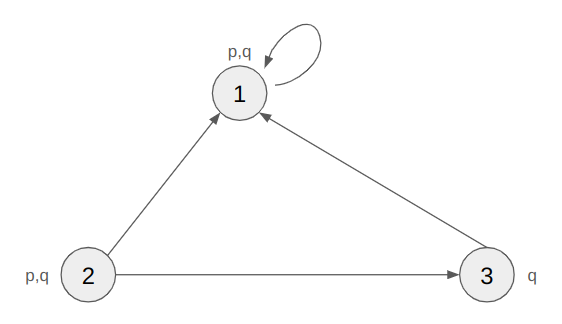
\includegraphics[width=0.75\textwidth]{images/maths/lmodal1.png}
    \caption{Un modelo $\mathcal{M}$.}
    \label{fig:lmodalimg1}
\end{figure}

Lo primero a destacar, es el conjunto de mundos que representan en el ejemplo, $W = \lbrace 1,2,3 \rbrace$. A continuación, se establecen las siguientes relaciones de accesibilidad entre mundos, donde la relación entre cada par sigue el camino de la flecha desde su inicio hasta la punta, quedando el conjunto $R = \lbrace (1,1), (2,1), (2,3), (3,1) \rbrace$. Para finalizar, sobre cada mundo se indica las proposiciones atómicas y su veracidad. En el caso del mundo 1 y 2, $p$ y $q$ son verdad, mientras que en el mundo 3 sólo lo es $q$. Finalmente, el modelo de Kripke para este ejemplo sería $\mathcal{M} = \langle W,R,V \rangle$, donde $V$ es la función de valoración presentada anteriormente, que explícitamente en este contexto quedaría definida de la siguiente manera:

\begin{align*}
    V(p) &= \lbrace 1,2 \rbrace \\
    V(q) &= \lbrace 1,2,3 \rbrace
\end{align*}

Algunos ejemplos de fórmulas interesantes y su verdad sobre el modelo de la figura ~\ref{fig:lmodalimg1} son las siguientes:
\begin{itemize}
    \item $\square p $ es verdadera en los mundos (1,3). En 2 no lo es, porque para que lo sea, debería ser verdadera $p$ para todos los mundos a los que se puede acceder desde 2, y en el mundo 3 eso no ocurre.
    \item $\diamondsuit p$ es verdadera en todos los mundos (1,2,3).
    \item $\square q$ es verdadera en todos los mundos.
    \item $\diamondsuit q$ es verdadera en todos los mundos.
    \item $\square(p \rightarrow q)$ es verdadera en todos los mundos.
\end{itemize}

\subsection{Relaciones de consecuencia lógica}\label{subsection:lmodalconsec}
En la lógica modal, a diferencia de en la lógica proposicional, las consecuencias lógicas dependen de la estructura con la que se esté trabajando. Se definen las nociones de \textit{consecuencia local} y \textit{consecuencia global}.

\vspace{0.5cm}
\noindent
\textbf{Consecuencia local}

Sean $\phi$ una fórmula modal y $\Sigma$ un conjunto de fórmulas modales. Se dice que $\phi$ es \textbf{consecuencia local} de $\Sigma$, si para todo modelo $\mathcal{M} = \langle W,R,V \rangle$ y para todo $w \in W$ tal que para cada $\psi \in \Sigma$, $\psi$ es satisfacible en $w$, ocurre que $\phi$ es satisfacible en $w$. Cuando esto sucede, se escribe $\Sigma \models_l \phi$.

\vspace{0.5cm}
\noindent
\textbf{Consecuencia global}

Sean $\phi$ una fórmula modal y $\Sigma$ un conjunto de fórmulas modales. Se dice que $\phi$ es \textbf{consecuencia global} de $\Sigma$, si para todo modelo $\mathcal{M} = \langle W,R,V \rangle$ y para todo $w \in W$ tal que para cada $\psi \in \Sigma$, $\mathcal{M} \models \psi$, ocurre que $\mathcal{M} \models \phi$. Cuando esto sucede, se escribe $\Sigma \models_g \phi$.

\vspace{0.5cm}
Una particularidad de las definiciones anteriores, es que cuando $\Sigma = \emptyset$, entonces se tiene que ambas consecuencias son equivalentes, es decir, para toda fórmula $\phi \in Form_{\mathcal{L}_{\mathcal{M}}}$:

\begin{align*}
    \models_l \phi \hspace{0.3cm} \Leftrightarrow \hspace{0.3cm} \models_g \phi
\end{align*}

\subsection{Sistemas lógicos modales}\label{subsection:lmodalsystems}
Dependiendo de las propiedades de la relación binaria escogida (véase ~\ref{subsection:binaryrel} ) para los modelos $\mathcal{M}$, se tiene un sistema lógico formal modal diferente, es decir, se definen diferentes axiomatizaciones. Aquí se realiza una clasificación de algunas de las que existen, dependiendo de las condiciones del marco $\mathcal{F}$:

\begin{itemize}
    \item \textbf{K}: no hay condiciones en el marco.
    \item \textbf{D}: $R$ es serial.
    \item \textbf{T}: $R$ es reflexiva.
    \item \textbf{B}: $R$ es reflexiva y simétrica.
    \item \textbf{K4}: $R$ es transitiva.
    \item \textbf{S4}: $R$ es reflexiva y transitiva.
    \item \textbf{S5}: $R$ es reflexiva, simétrica y transitiva.
\end{itemize}

\subsection{Lógica modal y TLA}\label{subsection:lmodalTLA}
La relación de la Lógica Temporal de Acciones (TLA) que se presentará en la sección ~\ref{section:TLA} con la lógica modal, se manifiesta en cómo TLA incorpora y extiende los principios de la semántica de Kripke. En TLA, los ``mundos'' de la lógica modal se corresponden con ``estados'' en un sistema, y las ``relaciones de acceso'' se transforman en ``transiciones'' entre estos estados. Estas transiciones representan cambios o acciones en el sistema, permitiendo modelar el comportamiento dinámico de sistemas complejos a lo largo del tiempo.

Un aspecto clave a destacar es que la axiomatización considerada para TLA se basará en el sistema modal D, cuya relación de acceso es ``serial'', lo que significa que para cada mundo (o estado en TLA), existe al menos un mundo accesible (o estado siguiente). Concretamente, esto se puede visualizar a través de este axioma del sistema lógico D modal:

\begin{align*}
    \square F \Rightarrow \diamondsuit F
\end{align*}



Esta característica es particularmente relevante en TLA, donde cada estado tiene un sucesor, reflejando la naturaleza continua y progresiva del tiempo y las acciones en sistemas dinámicos. En definitiva, en la siguiente sección se abordará con mayor rigor todos estos conceptos propios de TLA.

\section{Lógica Temporal de Acciones Proposicional (PTLA)}\label{section:TLA}
En esta sección se aborda el objetivo principal del capítulo: la Lógica Temporal de Acciones (TLA). Tras establecer las bases con la lógica proposicional, que simboliza el razonamiento humano en su forma más fundamental, se ha profundizado en la lógica modal, expandiendo el razonamiento a través de conceptos de \textit{necesidad} y \textit{posibilidad}. Esta extensión incluye la consideración de diversos mundos posibles, un aspecto esencial para entender la rica estructura de la TLA. Este marco conceptual sienta las bases para una comprensión integral de las lógicas temporales y se centra específicamente en la Lógica Temporal de Acciones, resaltando su capacidad para modelar dinámicas complejas a través de diferentes escenarios o ``mundos'', que serán nombrados como \textit{estados}.

La Lógica Temporal de Acciones fue definida por Leslie Lamport, en \cite{lamport1994temporal}, con el objetivo de verificar y especificar las propiedades de sistemas, particularmente concurrentes y distribuidos, mediante fórmulas. La motivación detrás de la definición de TLA por parte de Lamport radica en su convicción de que utilizar un razonamiento riguroso es la única manera de prevenir errores graves en algoritmo concurrentes. Esta percepción lleva al planteamiento de dos preguntas: ¿Por qué optar por una lógica en lugar de un lenguaje de programación convencional? ¿No sería más sencillo trabajar directamente con programas en lugar de fórmulas lógicas? La respuesta a ambas es no. ``\textit{La lógica es la formalización de las matemáticas de toda la vida, y las matemáticas de toda la vida son más simples que los programas}'', según comenta Lamport, no sin razón. Un lenguaje de programación puede usar términos matemáticos como \textit{función}, pero los constructos que representa no son tan simples como sus correspondientes conceptos matemáticos. Las funciones matemáticas son simples, mientras que en la mayoría de lenguajes de programación las funciones envuelven conceptos adicionales y complejos como \textit{expresión de retorno}, \textit{convención de llamada}, etc.

La naturaleza propia de la Lógica Temporal de Acciones está basada en la lógica de predicados, puesto que permite hacer razonamientos sobre estructuras complejas. Sin embargo, en esta sección se opta por presentar una axiomatización realizada por Martín Abadi \cite{abadi1990axiomatization}, usando para ello un enfoque proposicional de la TLA, denominada PTLA. Este enfoque proposicional representa una simplificación de TLA, reduciéndola a su forma más esencial y accesible. En PTLA, se utilizarán variables proposicionales en lugar de los términos más complejos de la lógica de predicados. Este enfoque es particularmente útil para introducir los conceptos fundamentales de las lógicas temporales sin la complejidad adicional de la lógica de predicados. En definitiva, el propósito es demostrar cómo los principios básicos de las lógicas temporales pueden ser utilizados para abordar y resolver problemas prácticos en el diseño y funcionamiento de sistemas informáticos, ofreciendo así una perspectiva valiosa sobre su aplicación práctica y relevancia en el mundo real.

\subsection{Modelos formales del tiempo}\label{subsection:TLAtime}
La Lógica Temporal de Acciones es \textbf{temporal} \cite{Pnueli1977TheTL}, \cite{gorankoRumberg2020temporal}. Eso quiere decir que los razonamientos realizados dependerán del \textbf{tiempo}. La primera cuestión a tratar es: ¿qué se entiende por \textit{tiempo}? ¿Qué ``tipo'' de tiempo se considera? La última pregunta se puede concretar y desglosar en otras varias: ¿Es un tiempo basado en \textit{intervalos} o en \textit{instantes}? ¿Es ese tiempo \textit{discreto}, \textit{denso}, o \textit{continuo}? ¿Hay \textit{principio}? ¿Y \textit{final}? Antes de poder hablar de PTLA, se muestran los dos tipos más básicos de modelos formales de tiempo, indicando al final cuál de los dos se escogerá para esta lógica particular.

\subsubsection{Modelos de tiempo basados en instantes}\label{subsubsection:TLAtimeinstant}
En estos modelos las entidades más primitivas son los \textbf{instantes de tiempo}, o también llamados \textbf{puntos en el tiempo}. Además, también se considera una relación binaria, escrita como $<$, para relacionar dichos puntos de tiempo. Considerando $t_a,t_b$  instantes de tiempo, se interpreta $t_a < t_b$ diciendo que $t_a$ es un instante de previo anterior a $t_b$. Por lo tanto, considerando $T$ como un conjunto no vacío de puntos temporales y $<$ una relación binaria sobre $T$, llamada \textbf{de precedencia}, el flujo temporal se puede representar como $\mathcal{T} = \langle T, <\rangle$. Sin embargo, es importante destacar que esta relación de precedencia no puede ser total. Esto se debe a la naturaleza discreta y secuencial de los modelos de tiempo basados en instantes, donde no todos los pares de instantes de tiempo pueden tener una relación directa de precedencia $<$ entre ellos. En lugar de ser total, la relación $<$ en estos modelos cumple con propiedades específicas de un \textbf{orden parcial}, como la irreflexividad, transitividad y asimetría (véase ~\ref{subsection:binaryrel}). Estas propiedades son esenciales para mantener la coherencia en la representación del flujo temporal.

Por otro lado, hay muchos modelos formales de tiempo basados en instantes. Los \textbf{modelos lineales} representan los instantes de tiempo como una linea, mientras que los \textbf{modelos lineales hacia atrás} permiten una representación ramificada, notando que el pasado es fijo (una linea), y el futuro es abierto (ramificándose en múltiples futuros posibles). Además, el ordenamiento temporal puede contener o no elementos mínimos o máximos, referentes al primer y último instante de tiempo, respectivamente.

Otra clasificación importante es la que se produce entre \textbf{modelos discretos}, \textbf{densos}, y \textbf{continuos}. Los modelos discretos \textit{hacia adelante} indican que, cada instante de tiempo que tiene un sucesor, éste siempre tiene un sucesor inmediato correspondiente. Formalmente, $\forall t \in T, \exists t' \in T \text{ tal que } t < t'$. En los modelos densos, por el contrario, entre dos instantes de tiempo subsiguientes cualesquiera, hay otro instante. Por otra parte, en los modelos continuos el orden temporal no sólo debe ser denso, sino que además, todo conjunto no vacío de instantes de tiempo que tiene un límite superior tiene un límite superior mínimo.

\subsubsection{Modelos de tiempo basados en intervalos}\label{subsubsection:TLAtimeinterval}
Este tipo de modelos aparecen cuando se necesita realizar razonamientos sobre eventos con duración. En este caso, las entidades primitivas son los \textbf{intervalos}. En estos modelos se presupone un tiempo lineal, aunque a diferencia de los modelos basados en instantes, aquí se pueden definir muchas más relaciones. Por todo ello, formalmente se define este flujo temporal como $\mathcal{T} = \langle T,<,\subset,O \rangle$, donde se tienen las relaciones binarias de precedencia $<$, inclusión $\subset$, y superposición $O$. No se entrará en más detalles acerca de este tipo de modelos.

\subsubsection{El modelo de tiempo de PTLA}\label{subsubsection:TLAtimedecision}
El modelo de tiempo $\mathcal{T} = \langle T, < \rangle$ considerado para la lógica temporal de acciones tendrá las siguientes características:
\begin{enumerate}
    \item \textbf{Basado en instantes}: En muchos sistemas, especialmente en informática y sistemas distribuidos, es crucial modelar y razonar sobre eventos en momentos específicos. Un modelo basado en instantes permite la representación precisa de cuándo ocurren acciones o cambios de estado. Este enfoque facilita el análisis preciso de secuencias de eventos y la sincronización entre acciones. Permite establecer relaciones causales y temporales claras entre eventos individuales.
    \item \textbf{Lineal}: Un modelo temporal lineal implica que para cualquier momento dado, hay un único ``futuro'' y un único ``pasado''. La linealidad simplifica el razonamiento sobre secuencias de eventos. Facilita la comprensión de las relaciones temporales, como ``antes'' y ``después'', y es más intuitiva para modelar muchos tipos de sistemas.
    \item \textbf{Discreto}: El tiempo se considera como un conjunto de momentos distintos y separados (por ejemplo, ``ticks'' de un reloj). Esto es particularmente adecuado para sistemas informáticos y digitales, donde las operaciones se realizan en pasos discretos.
    \item \textbf{Tiene un comienzo}: Siempre se considerará un punto de partida concreto: el \textit{instante 0}.
\end{enumerate}

\subsection{Estados. Comportamientos. Sistemas dinámicos}\label{subsection:TLAsystems}
El propósito de la Lógica Temporal de Acciones Proposicional es razonar sobre sistemas, especialmente concurrentes. Una aproximación unificada de programas secuenciales y concurrentes es lo que se denomina como \textit{sistema dinámico discreto}. Un \textbf{sistema dinámico discreto} $\mathcal{D}$ es un triple $\langle S, R, s_0 \rangle$ donde:

\begin{itemize}
    \item $S$ es el conjunto de estados del sistema (posiblemente infinito). Cada elemento, naturalmente, se denomina \textbf{estado}.
    \item $R$ es la relación de transición entre un estado y sus posibles sucesores. $R$ evidentemente, es una relación binaria que involucra sólo a dos estados.
    \item $s_0$ es el estado inicial.
\end{itemize}

En la sección ~\ref{subsec:concurrentatomic} ya se hizo una ligera mención a la noción de estados, transiciones entre ellos, y su relación con los programas concurrentes. Para dar una comprensión más detallada y clara apoyada en el concepto temporal, un estado en el contexto de un programa se puede visualizar como una ``instantánea'' en un punto específico del tiempo, denotado como $t = 0, 1, \ldots$. Esta instantánea captura y preserva todos los aspectos relevantes del sistema en ese momento, incluyendo los valores de sus variables y el estado de sus componentes internos. Cada estado, por lo tanto, refleja una configuración completa del sistema, proporcionando una base para entender y rastrear cómo y cuándo ocurren los cambios a lo largo del tiempo. 

Formalmente, se puede definir un estado como una función que asigna valores a todas las variables, donde una \textit{variable}  es un identificador que representa una propiedad específica o un atributo del sistema. Esta propiedad puede variar con el tiempo y es crucial para determinar el estado del sistema en cualquier momento dado. Las variables pueden representar una amplia gama de datos, como números, valores de verdad, o cadenas de texto, y son fundamentales para describir las características y el comportamiento del sistema. En otras palabras, $s$ por tanto queda determinada como:

\begin{align*}
    s : Var &\to Val \\
    x &\mapsto s(x)
\end{align*}

donde $Var$ y $Val$ denotan el conjunto de variables y de valores, respectivamente. El conjunto de valores puede contener diferentes tipos de elementos como números naturales, reales, e incluso cadenas de caracteres.

Por otra parte, un \textbf{comportamiento} o \textbf{ejecución} es una sucesión de estados (posiblemente infinita), escribiéndose:

\begin{align*}
    \sigma = \langle s_0, s_1, s_2, \ldots \rangle
\end{align*}

La relación de transición entre estados es no determinista en general (es decir, dado un estado $s$, su siguiente no tiene por qué ser siempre el mismo), por lo que diferentes secuencias de ejecución son posibles. Al conjunto de todos los posibles comportamientos de un sistema se escribe como $S^\infty$.

Para referirse al estado concreto de un comportamiento de un sistema, $\sigma \in S^\infty$, en un instante de tiempo $t$ concreto, se escribe $\sigma_t = s_t$. También, para referirse a la secuencia de estados que siguen al estado del sistema en el instante $t$, se escribe $\sigma^{+t} = \langle s_{t+1}, s_{t+2}, \ldots \rangle$. Se dice que un comportamiento $\sigma$ de un sistema está \textbf{detenido} cuando $\sigma_t = \sigma_0$, para todo instante de tiempo $t$. En caso contrario, se denota por $\mu(\sigma)$ como al primer instante de tiempo $t$ donde $\sigma_t \neq \sigma_0$.

\subsection{Acciones}\label{subsection:TLAactions}
La Lógica Temporal de Acciones se basa en el concepto de \textit{acciones}. En el contexto proposicional de esta lógica, una \textbf{acción} se define como una proposición $A$ que relaciona el estado actual de una variable con su estado siguiente. En una proposición $A$, se establece una relación entre los valores de las variables en el estado $s$ y los valores correspondientes en el estado $t$ (indicados por la prima). Esta relación puede cumplirse o no cumplirse para cualquier par de estados $s$ y $t$.

Por ejemplo, se considera la acción $A_0 := $``$x' = x+1$''. Aquí, $x$ es una variable que tiene un valor actual en el estado $s$, y $x'$ denota el estado de la variable en el instante de tiempo inmediatamente posterior, que es el estado $t$. El operador $'$ desempeña un papel crucial en la definición sintáctica de PTLA, ya que permite formular afirmaciones sobre los estados futuros de las variables.

La lectura de la acción se puede realizar de la siguiente manera: ``en el estado siguiente ($t$), el valor de $x$ será incrementado en una unidad con respecto a su valor actual ($s$)''.

Es importante destacar que una acción $A$ puede ser verdadera para diferentes pares de estados $s$ y $t$, dependiendo de la acción específica. Por ejemplo, en el caso de la acción ``$x \text{ es par} \Rightarrow x' \text{ es par}$'', cualquier estado $t$ donde $x$ también sea par satisfaldrá la acción, lo que significa que hay múltiples estados posibles posteriores a $s$ una vez que se ejecuta la acción $A$. En resumen, una acción puede definirse como una proposición que relaciona el estado actual con el estado siguiente, y esta relación puede variar según el contexto de la acción.


\subsection{El lenguaje PTLA}\label{subsection:TLAlanguage}
Ahora, ya se puede hacer una definición formal del Lenguaje Proposicional Temporal de Acciones (PTA). Un \textbf{Lenguaje PTA} $\mathcal{L}_{TA}$ es una cuádrupla $(O,C,\mathcal{A},\mathcal{P})$ donde:

\begin{itemize}
    \item $O = \lbrace \neg, \land, \lor, \Rightarrow, \equiv \square, \diamondsuit \rbrace$ como el conjunto de conectivas u operadores lógicos. Aquí, el conjunto de conectivas primario considerado será $\lbrace \neg, \land, \lor \rbrace$, junto con los operadores modales $\lbrace \square, \diamondsuit \rbrace$
    \item $C = \lbrace \bot \rbrace$ es el conjunto de constantes proposicionales.
    \item $\mathcal{A}$ es el conjunto de \textbf{variables de acción}. Ejemplos son $A_0,A_1,A_2,\ldots$. Las variables de acción representan a proposiciones atómicas acerca de los estados de una variable, como se ha discutido en la sección anterior.
    \item $\mathcal{P}$ es el conjunto se variables proposicionales. Ejemplos son $P_0,P_1,P_2,\ldots$
\end{itemize}

Para poder trabajar con comodidad de aquí en adelante, se denomina \textbf{predicado de estado} a una combinación de los símbolos proposicionales con operadores lógicos, incluyendo también las constantes. Se escribirá como $Pred_{\mathcal{L}_{TA}}$ al conjunto de los predicados de estado del lenguaje. Si $P$ es un predicado de estado, se denota por $P'$ al \textbf{predicado de estado prima}, dando una afirmación sobre los componentes de $P$ pero en el estado inmediatamente posterior. Por otra parte, una \textbf{acción} será una combinación de predicados de estado, predicados de estado prima, y variables de acción, y se $Act_{\mathcal{L}_{TA}}$ es el conjunto de los acciones del lenguaje. Normalmente una acción se escribirá como $A,B,C, \ldots$.

Los términos de \textit{expresión},\textit{fórmula} y \textit{subfórmulas} siguen manteniendo las definiciones de la lógica proposicional y de la lógica modal. Sin embargo, ahora hay nuevas fórmulas a considerar. Son fórmulas de la lógica PTLA:

\begin{itemize}
    \item los predicados de estado.
    \item $[A]$, $\langle A \rangle \equiv \neg[\neg A]$, donde $A$ es una acción. El propósito de estas fórmulas quedará más claro cuando se introduzca su semántica.
    \item Si $F,G$ son fórmulas:
    \begin{itemize}
        \item $\neg F$, $F \land G$, $F \lor G$, son fórmulas.
        \item $\square F$, $\diamondsuit F \equiv \neg \square \neg F$, son fórmulas. A diferencia de en la lógica modal, ahora se leen ``siempre $F$'' y ``posible $F$'', respectivamente.
    \end{itemize}
\end{itemize}

Para poder entender mejor estas nuevas definiciones, se presenta un ejemplo. Sean $P_0,P_1$ variables proposicionales, y $A_0$ una variable de acción. Se definen las siguientes fórmulas:

\begin{itemize}
    \item $P_0 := x = 0$, y se lee como ``el valor de la variable $x$ es 0''.
    \item $P_1 := x = 1$, y se lee como ``el valor de la variable $x$ es 1''.
    \item A partir de $P_1$, se define $P_1' := x' = 1$, y se lee como ``el valor de la variable $x$ en el estado siguiente es 1''.
    \item $A_0 := x' = x+1$, y se lee como ``en el estado siguiente, el valor de la variable $x$ valdrá $1$ unidad más que el valor actual''. 

    \item $P_0 \land A_0 \Rightarrow P_1'$. Esto quiere decir que: ``Si el valor actual de $x$ es 0 ($P_0$) y ocurre la acción de incrementar $x$ en $1$, entonces en el estado siguiente el valor de $x$ será 1 $(P_1')$''.
\end{itemize}

La idea, introducida en ~\ref{subsection:lpropTLA}, es que las fórmulas TLA sirvan para especificar las propiedades de un programa concurrente, combinando el uso de predicados de estado con acciones que alteran los estados del sistema. Este enfoque resulta particularmente útil para la verificación de programas, donde las secuencias de eventos y las condiciones de sincronización son críticas.

\subsection{Semántica}\label{subsection:TLAsemantics}
El siguiente paso para poder determinar adecuadamente la lógica es dotar de significado a las fórmulas anteriormente descritas. La lógica modal es la que establece las bases para describir la semántica. En primer lugar, se entiende por \textbf{interpretación} al par $(S,I)$ donde:
\begin{itemize}
    \item $S$ es el \textit{espacio de estados}, conjunto no vacío ya introducido en la sección ~\ref{subsection:TLAsystems}, que contiene los posibles estados de un sistema dinámico discreto, como los programas.
    \item $I$ representa a un par de aplicaciones, $(I_\rho,I_\alpha)$ que asignan a cada variable proposicional $P_i, i \in \lbrace 0,1, \ldots \rbrace$ un subconjunto del espacio de estados $S$, y a cada variable de acción $A_i, i \in \lbrace 0,1, \ldots \rbrace$ un subconjunto de $S \times S$, respectivamente.
\end{itemize}

La idea intuitiva de los conjuntos que asignan las aplicaciones anteriores es la siguiente: $I_\rho(P_i)$ es el subconjunto de todos los estados donde $P_i$ es verdadera, noción estrechamente relacionada con lo introducido en ~\ref{subsection:lmodalsemantic}; mientras que  $I_\alpha(A_i)$ es el conjunto de pares de estados relacionados por $A_i$.

De manera análoga a lo que se realizó en ~\ref{subsection:lpropsemantic}, ahora se puede extender la definición de las funciones de interpretación para objetos sintácticos más complejos. Formalmente, las aplicaciones quedarían determinadas de la siguiente manera:

\begin{align*}
    I_\rho: Pred_{\mathcal{L}_{TA}} &\to S \\
    P &\mapsto I_\rho(P) \subset S
\end{align*}

\begin{align*}
    I_\alpha: Act_{\mathcal{L}_{TA}} &\to S \times S\\
    A &\mapsto I_\alpha(A) \subset S \times S
\end{align*}

\noindent
En el caso de los predicados de estado:

\begin{align*}
    I_\rho(\bot) &\triangleq \emptyset  \\
    I_\rho(\neg P) &\triangleq S \setminus I_\rho(P) \\
    I_\rho(P \land Q) &\triangleq I_\rho(P) \cap I_\rho(Q) \\
    I_\rho(P \lor Q) &\triangleq I_\rho(P) \cup I_\rho(Q)
\end{align*}

La forma de extender la interpretación a predicados de estado es bastante intuitiva. En el primer caso, la interpretación de la negación del predicado se relacionará con todos aquellos estados donde el predicado $P$ es falso, mientras que en el caso de la conjunción se contempla el conjunto de estados donde ambos predicados son verdaderos a la vez. Por otro lado, es evidente que para la conjunción de predicados de estado es suficiente con considerar la unión de los estados donde $P$ y $Q$ son verdad. Ahora, queda extender las interpretaciones a las acciones:


\begin{align*}
    I_\alpha(P) &\triangleq I_\rho(P) \times S \\
    I_\alpha(P') &\triangleq S \times I_\rho(P) \\
    I_\alpha(\neg A) &\triangleq (S \times S) \setminus I_\alpha(A) \\
    I_\alpha(A \land B) &\triangleq I_\alpha(A) \cap I_\alpha(B) \\
    I_\alpha(A \lor B) &\triangleq I_\alpha(A) \cup I_\alpha(B)
\end{align*}

La extensión de la función de interpretación a las acciones también es intuitiva. Lo primero que hay que recordar es que, los predicados de estado, también pueden ser considerados acciones. La interpretación de un predicado mediante $I_\alpha$ relaciona el subconjunto de espacios donde $P$ es verdadera con el espacio de estados completo. Esto significa que, desde cualquier estado donde $P$ es verdadero, la transición puede ir hacia cualquier otro estado del sistema, reflejando la idea de que la acción asociada a $P$ puede ocurrir en cualquier transición desde un estado donde $P$ es verdadero. En el caso de una acción que involucre al predicado de estado prima $P'$,  se considera la transición a estados donde $P$ será verdadero en el siguiente instante de tiempo, desde cualquier estado actual. Esto refleja la posibilidad de llegar a un estado donde $P$ es verdadero, partiendo de cualquier estado previo. En el caso de la negación de una acción, conjunción y disyunción de acciones el razonamiento es similar al dado para los predicados de estado.

\subsubsection{Modelos. Fórmulas satisfacibles y válidas}\label{subsubsection:TLAvalidForms}
Un \textbf{modelo} es un triple $\mathcal{M} =  \langle S,I,\sigma \rangle$, donde $(S,I)$ es una interpretación y $\sigma \in S^\infty$ es un comportamiento sobre $S$. La definición de \textbf{fórmula verdadera} en un modelo determinado se define inductivamente como sigue:

\begin{align*}
    \mathcal{M} \models P_j &\triangleq \sigma_0 \in I_\rho(P_j), \hspace{0.2cm} j \in \lbrace 0,1,\ldots \rbrace \\
    \mathcal{M} \models [A] &\triangleq \sigma \text{ está detenido ó } (\sigma_0,\sigma_{\mu(\sigma)}) \in I_\alpha(A) \\
    \mathcal{M} \models \bot &\triangleq \bot \\
    \mathcal{M} \models \neg F &\triangleq M \not \models F \\
    \mathcal{M} \models F \land G &\triangleq \mathcal{M} \models F \text{ y } \mathcal{M} \models G \\
    \mathcal{M} \models \square F &\triangleq \forall i \in \lbrace 0,1,2,\ldots \rbrace, \langle S,I,\sigma^{+i}\rangle \models F
\end{align*}

Se dice que $F$ es una \textbf{fórmula satisfacible} si existe un modelo $M = \langle S,I,\sigma \rangle$ de modo que $\mathcal{M} \models F$. Además, se dice que $F$ es una \textbf{fórmula válida} si $F$ es satisfacible para todo modelo $M$, y en ese caso, se escribe $\models F$.

\subsection{Axiomas de PTLA}\label{subsection:TLAaxioms}
Una lógica consta de una serie de axiomas que se asumen como verdaderas, y un conjunto de reglas que permiten hacer además algunas operaciones para deducir la veracidad de otras fórmulas del lenguaje. En este caso, Martín Abadi realizó una axiomatización de la Lógica Temporal de Acciones Proposicional, teniendo en cuenta una axiomatización basada en el sistema lógico D (ver ~\ref{subsection:lmodalsystems}). La lista de axiomas \footnote{El símbolo $\vdash$ se utiliza en la lógica para representar una relación de deducción o derivación. En el contexto de los sistemas lógicos, cuando se escribe $\vdash F$, significa que la fórmula $F$ es derivable o deducible a partir de un conjunto de axiomas y reglas de inferencia. En el caso de los axiomas, $\vdash$ se usa para enfatizar que se consideran verdaderos dentro del sistema lógico, formando la base de las derivaciones posteriores. No implica necesariamente que $F$ sea verdadera en un sentido absoluto, sino que es verdadera bajo las premisas y dentro del marco del sistema lógico aplicado.} es la siguiente:

\begin{enumerate}
    \item $ \vdash \square (F \Rightarrow G) \Rightarrow (\square F \Rightarrow \square G) $
    
    Este axioma indica la transmisión de la propiedad ``ser siempre verdadero'' a través de una implicación lógica.
    
    \item $ \vdash \square F \Rightarrow F $

    Este axioma refleja la idea de que la verdad perpetua de una fórmula, en particular lo es en el momento presente.
    
    \item $ \vdash \square F \Rightarrow \square\square F $

    Este axioma refuerza la idea de persistencia de verdad a través del tiempo.
    
    \item $ \vdash \square (\square F \Rightarrow G) \lor \square(\square G \Rightarrow F) $

    Este axioma es una manera clásica de expresar que el tiempo es lineal y que dos instantes cualesquiera en el futuro están ordenados. En el contexto del tiempo lineal sugiere que, en cualquier par de eventos en el tiempo, existe una relación de precedencia o causalidad entre ellos. Es decir, si un evento es perpetuo, esto afecta a la veracidad del otro, y viceversa.
    
    \item $ \vdash \square (\square(F \Rightarrow \square F)\Rightarrow F) \Rightarrow (\diamondsuit \square F \Rightarrow F) $

    Este axioma representa la naturaleza de que el tiempo es discreto. $\square(F \Rightarrow \square F)$ significa que siempre es cierto que si $F$ es verdadero, entonces $F$ será siempre verdadero en el futuro, indicando así una ``persistencia'' de $F$. Ahora, $\square (\square(F \Rightarrow \square F)\Rightarrow F)$ indica que si la persistencia futura de $F$ garantiza $F$, entonces $F$ debe ser cierta en el presente. Por otro lado $\diamondsuit \square F \Rightarrow F$ dice que si es posible que $F$ sea perpetuamente verdadera en el futuro, entonces $F$ es verdadera ahora. En esencia, la relación entre las dos partes establece que si la garantía de que una propiedad se mantendrá en el futuro significa que debe ser cierta ahora, entonces el hecho de que esa propiedad pueda ser perpetua en algún punto futuro también significa que debe ser cierta ahora.
    
    \item Si $\vdash F $ entonces $\vdash \square F $.

    Este axioma es un principio de generalización que indica que si una fórmula $F$ es verdadera, entonces siempre es verdadera.
    
    \item Si $ F $ es una instancia de una tautología proposicional entonces $\vdash \square F $.
    
    \item Si $ \vdash F $ y $ \vdash F \Rightarrow G $ entonces $ \vdash G $.

    Este axioma es un principio básico de la inferencia lógica.
    
    \item $ \vdash \lbrack \bot \rbrack \Rightarrow \lbrack A \rbrack $

    Este axioma maneja casos límite en la lógica de acciones. Si una acción imposible es verdadera, entonces cualquier acción $A$ es verdadera.
    
    \item $ \vdash \lbrack \bot \rbrack \Rightarrow \lbrack P \rbrack = P $

    Este axioma sirve para mantener la consistencia en el tratamiento de acciones imposibles.
    
    \item $ \vdash \lbrack \bot \rbrack \Rightarrow \lbrack \neg A \rbrack \equiv \neg \lbrack A \rbrack $

    Este axioma establece que bajo una acción imposible, la negación de una acción $A$ es equivalente a la negación de $A$ como una acción.
    
    \item $ \vdash \lbrack A \land B \rbrack \equiv \lbrack A \rbrack \land \lbrack B \rbrack $

    Este axioma indica la verdad de una acción definida por la conjunción de dos acciones.
    
    \item $ \vdash \lbrack (\neg P)' \rbrack \equiv \neg \lbrack P' \rbrack $

    \item $ \vdash \lbrack (P \land Q)' \rbrack \equiv \lbrack P' \rbrack \land \lbrack Q' \rbrack $
    \item $ \vdash \square P \Rightarrow \lbrack P' \rbrack $

    Este axioma indica que si un predicado $P$ es siempre verdadero, entonces la afirmación sobre $P$ en el estado siguiente ($P'$) también es verdadera.
    
    \item $ \vdash \square( P \Rightarrow ((\lbrack P' \rbrack \land G) \lor \square G )) \Rightarrow (([P'] \land G) \Rightarrow \square G)$

    Este axioma se puede ver como sigue: supongamos que siempre que $P$ sea verdadero, entonces o bien $G$ es verdadero y $P$ sobrevive al siguiente cambio de estado, o $G$ es verdadero para siempre. Esto implica que $G$ se mantiene verdadero mientras $P$ se mantiene verdadero, y se vuelve verdadero para siempre si $P$ deja de ser verdadero. Por lo tanto, si $G$ es verdadero inicialmente y $P$ es verdadero después del primer cambio de estado, entonces $G$ es siempre verdadero. 
    
    En definitiva es útil para modelar situación donde la verdad de una condición o propiedad depende de la persistencia de otra a lo largo del tiempo. Por ejemplo, en sistemas de software, podría utilizarse para modelar cómo diversas condiciones deben mantenerse mientras otras condiciones sigan siendo verdaderas.
\end{enumerate}

\subsubsection{Algunas consecuencias de los axiomas}\label{subsubsection:TLAconseq}
Algunas consecuencias de los axiomas presentados para la lógica temporal de acciones proposicional son las citadas a continuación:

\begin{enumerate}
    \item $\vdash [\bot] \Rightarrow (F \equiv \square F) \land (F \equiv \diamondsuit F)$

    Esta fórmula indica que, una vez se ha detenido la ejecución, todas las características permanecen permanentes, significando que $F$,$\square F$ y $\diamondsuit F$ son equivalentes, para toda $F$.
    
    \item $\vdash \langle P' \rangle \Rightarrow \diamondsuit P$

    En palabras, si la ejecución no se ha detenido y la siguiente acción es P', entonces P eventualmente sucederá. Esta fórmula indica una forma sencilla de probar propiedades de vivacidad.

    
    \item $\vdash P \land \square(P \Rightarrow [P']) \Rightarrow \square P$

    Esta fórmula es una consecuencia de instanciar $G$ por $P$ en el Axioma 16.
    
    \item $\vdash [P'] \land \diamondsuit G \Rightarrow G \lor \diamondsuit (P \land \diamondsuit G)$

    Este teorema es una consecuencia del Axioma 16. Dice que si la acción $P'$ va a tener lugar (siempre que la ejecución no se haya detenido) y $G$ debe darse eventualmente, entonces o $G$ es verdadera ahora, o $P$ sucederá eventualmente y $G$ sucederá más tarde.
    
    \item $\vdash (P \land \diamondsuit G \land \square (P \land \diamondsuit G \Rightarrow [P'])) \Rightarrow \diamondsuit (P \land G)$

    Esta fórmula es el dual del Axioma 16. En otras palabras, mientras que el Axioma 16 se enfoca en la persistencia de una condición y su impacto en otra, esta fórmula considera las condiciones necesarias para que dos propiedades se cumplan eventualmente en el futuro.
\end{enumerate}

\subsection{Solvencia y completitud}\label{subsection:TLAcompleteness}
En el estudio de cualquier sistema lógico, dos propiedades fundamentales a considerar son la solvencia (o corrección) y la completitud. Estos conceptos son cruciales para evaluar la robustez y confiabilidad del sistema lógico, especialmente en un contexto como el de PTLA, donde se trata de capturar y razonar sobre el comportamiento de sistemas concurrentes y distribuidos.

La \textbf{solvencia} de un sistema lógico se refiere a la garantía de que todas las fórmulas que pueden ser deducidas dentro del sistema son verdaderas en todos los modelos del sistema. En el contexto de PTLA, esto significa que si una fórmula $F$ puede ser deducida $\vdash F $, entonces $F$ debe ser verdadera en cada modelo de PTLA $ \mathcal{M} \models F $ para todo modelo $\mathcal{M}$. La solvencia asegura que el sistema no permite derivar conclusiones falsas o inconsistentes a partir de sus axiomas y reglas de inferencia.

La \textbf{completitud}, por otro lado, se refiere a la capacidad del sistema lógico para derivar todas las fórmulas verdaderas en todos los modelos. En PTLA, un sistema es completo si, para cada fórmula $ F $ que es verdadera en todo modelo $ \mathcal{M} \models F $ para todo modelo $ \mathcal{M} $, existe una derivación de $ F $ dentro del sistema $ \vdash F $. La completitud asegura que el sistema es capaz de capturar todas las verdades que se pueden expresar en su lenguaje.

En la Lógica Temporal de Acciones Proposicional, se verifican dos teoremas fundamentales relacionados con estos conceptos:

\begin{teorema}
    Sea $G$ una fórmula. Si $G$ no es deducible, entonces $\neg G$ tiene un modelo.
\end{teorema}

\begin{teorema}
    \textbf{Solvencia y complitud}: Sea $F$ una fórmula. $\vdash F \Leftrightarrow \hspace{0.1cm} \models F$.
\end{teorema}

\subsection{Ejemplo práctico de especificación con PTLA}\label{subsection:PTLAExample}
Para poder en valor todo el estudio matemático realizado a lo largo de este capítulo, se ofrecerá un ejemplo muy sencillo de cómo la Lógica Temporal de Acciones puede ayudar a la especificación de programas, entre ellos los concurrentes, que son el objeto de estudio global de todo el proyecto tanto teóricamente como en la práctica.

El siguiente ejemplo denota un simple programa que cuando se ejecuta, permanece incrementando las dos únicas variables que posee $x,y$ inicializadas a 0, eligiendo de forma no determinística cuál incrementar.

\begin{figure}[ht]
\centering
\begin{lstlisting}[basicstyle=\ttfamily\small, frame=single]
    var natural x,y = 0;
    do 
       < true -> x := x + 1 >
       [ ]
       < true -> y := y + 1 >
    od
\end{lstlisting}
\caption{Ejemplo de programa para especificación: Incremento.}
\label{fig:TLAincrement}
\end{figure}

\begin{figure}[h]
    \centering
    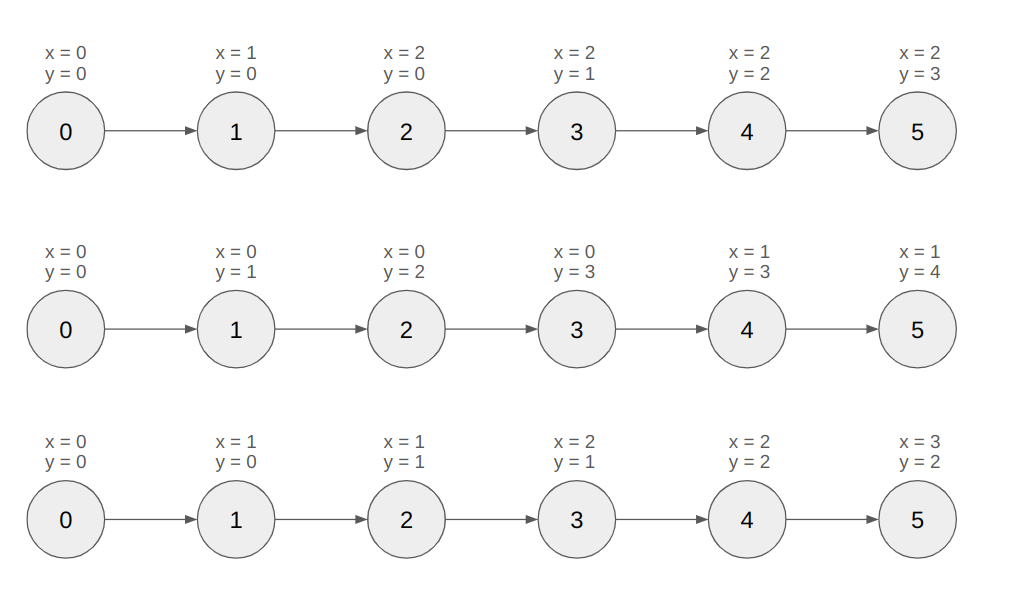
\includegraphics[width=0.9\textwidth]{images/maths/ptla1.png}
    \caption{Diferentes comportamientos del programa Incremento.}
    \label{fig:TLAincrementBehav}
\end{figure}

La figura ~\ref{fig:TLAincrementBehav} culmina todos los conceptos tratados hasta el momento en este capítulo. En primer lugar, se dispone de un conjunto posiblemente infinito de estados $S$, que están representados por los nodos o círculos azules, y que indican el valor de las variables en un instante de tiempo $t$ determinado, esto es, en el estado 0 se indica el valor de las variables en el instante 0, y así sucesivamente. Además, desde el punto de vista de la lógica modal, se puede ver a $S$ como el conjunto de todos los mundos posibles, y su relación entre ellos, que es de tipo serial, pues cada estado (o ``mundo'') tiene al menos un estado sucesor (o ``mundo accesible''), en consonancia con lo mencionado en la axiomatización de PTLA. Para finalizar, se refleja la propiedad de no determinismo de dicha relación, pues aunque siempre se relacione el estado $s_1$ con $s_2$, su naturaleza en las tres diferentes secuencias no es la misma, debido al funcionamiento intrínseco del programa de elegir indiscriminadamente qué variable incrementar, propiciando diferentes comportamientos.

En primer lugar, se recuerda que en ~\ref{subsection:TLAtime} se definió el modelo temporal sobre el que se sustenta el razonamiento sobre los sistemas concurrentes. $\mathcal{T} = \langle T, < \rangle$ es el modelo formal elegido donde $<$ es un orden parcial. Los instantes de tiempo de ejecución del programa empiezan en el segundo $0$, evolucionando discreta y linealmente. A continuación, se puede denotar por $\mathcal{D} = \langle S, R, s_0 \rangle$ al sistema dinámico que representa el programa de incremento, donde $R$ es una relación binaria serial, pues partiendo de un estado concreto, siempre se puede acceder a otro estado siguiente. En la figura ~\ref{fig:TLAincrementBehav} se representan tres comportamientos diferentes del programa: $\sigma_0, \sigma_1, \sigma_2 \in S^\infty$, respectivamente.

Se llamará $\Phi$ a la fórmula que especificará el programa al completo. En primer lugar, se puede especificar el estado inicial del programa utilizando las siguientes proposiciones y construyendo la fórmula (concretamente el predicado de estado) $Init_{\Phi}$:

\begin{align*}
    P_0 &\triangleq x = 0 \\
    P_1 &\triangleq y = 0 \\
    Init_{\Phi} &\triangleq P_0 \land P_1
\end{align*}

\noindent
Lo que deja a la fórmula $\Phi$ por el momento como:

\begin{align*}
    \Phi \triangleq Init_{\Phi}
\end{align*}

A continuación, por las características del programa se pueden tomar dos diferentes \textit{acciones}: o incrementar en una unidad la variable $x$, o hacer lo propio con la variable $y$. Esto se puede escribir de la siguiente manera:

\begin{align*}
    A_0 &\triangleq x' = x+1 \hspace{0.3cm} &\text{(Incrementar x)} \\
    A_1 &\triangleq y' = y \hspace{0.3cm} &\text{(Dejar sin cambios y)}\\
    A_2 &\triangleq x' = x \hspace{0.3cm} &\text{(Dejar sin cambios x)} \\
    A_3 &\triangleq y' = y+1 \hspace{0.3cm} &\text{(Incrementar y)} \\
    A &\triangleq A_0 \land A_1 \hspace{0.3cm} &\text{(Incrementar x, no modificar y)} \\
    B &\triangleq A_2 \land A_3 \hspace{0.3cm} &\text{(No modificar x, incrementar y)} \\
    \mathcal{A} &\triangleq A \lor B \hspace{0.3cm} &\text{(Ocurre la acción A u ocurre la acción B)}
\end{align*}

Ahora, se puede actualizar la fórmula $\Phi$ que especifica al programa añadiendo la siguiente fórmula:

\begin{align*}
    \Phi \triangleq Init_{\Phi} \land [\mathcal{A}]
\end{align*}

Con esto, lo que estamos diciendo es que, para cualquier punto en el comportamiento del programa después de $Init_{\Phi}$ , si el programa no se ha detenido, entonces la acción que sigue es o incrementar $x$ (acción $A$) o incrementar $y$ (acción $B$), y estas son las únicas transiciones posibles. La fórmula $\Phi$ tiene modelos que la satisfacen, concretamente:

\begin{align*}
    \langle S, I, \sigma_i \rangle \models \Phi, \hspace{0.3cm} i \in \lbrace 0,1,2 \rbrace
\end{align*}

En particular, es algo que siempre ocurre en todos los estados a partir del estado inicial (siempre que el programa no se haya detenido). En otras palabras, es una fórmula que se satisface para todo modelo considerado, por lo que se puede escribir la fórmula:

\begin{align*}
    \Phi \triangleq Init_{\Phi} \land \square[\mathcal{A}]
\end{align*}

Así, se indica que la ejecución de la acción se satisface en todos los subsiguientes estados después del inicio, sin excepción. La fórmula $\Phi$ ya presenta una propiedad para el programa, concretamente la \textit{propiedad de seguridad}, garantizando que nunca ocurrirán otras acciones no especificadas, lo que podría ser considerado como un ``comportamiento malo''. En otras palabras, el programa está restringido a comportarse de manera segura tal como se ha definido por las acciones.

\section{Otros sistemas lógicos para verificación de sistemas}\label{section:otherlogics}
La Lógica Temporal de Acciones en definitiva es un excelente sistema lógico formal para razonar sobre las propiedades de los sistemas concurrentes. Sin embargo, no es el único sistema lógico formal que se utiliza, sino que hay una gran variedad de ellos que pueden ser utilizados para ese mismo fin. A continuación, se mencionan brevemente comparando sus enfoques con el de TLA:

\begin{itemize}
    \item \textbf{Lógica Temporal Lineal (LTL)}:
    \begin{itemize}
        \item \textit{Enfoque}: Se centra en el comportamiento de los sistemas a lo largo del tiempo, permitiendo hacer afirmaciones sobre secuencias de estados en el futuro.
        \item \textit{Comparación con TLA}: TLA se orienta hacia acciones y transiciones entre estados, mientras que LTL se enfoca en las propiedades de los estados a lo largo del tiempo.
    \end{itemize}
    
    \item \textbf{Lógica Temporal de Árbol Computacional (CTL)}:
    \begin{itemize}
        \item \textit{Enfoque}: Permite expresar propiedades sobre árboles de ejecución, representando múltiples futuros posibles desde un mismo estado.
        \item \textit{Comparación con TLA}: CTL es más adecuada para sistemas no deterministas con varias posibilidades de evolución, a diferencia de TLA que es más lineal.
    \end{itemize}
    
    \item \textbf{Lógica de Hoare \footnote{En particular, este sistema lógico formal es el que se enseña en la asignatura de \textit{Sistemas Concurrentes y Distribuidos}.}}: 
    \begin{itemize}
        \item \textit{Enfoque}: Se centra en la corrección de programas individuales mediante tripletas que relacionan estados iniciales y finales con una instrucción. 
        \item \textit{Comparación con TLA}: Mientras la Lógica de Hoare es más adecuada para programas secuenciales, TLA es más efectiva en sistemas concurrentes y distribuidos.
    \end{itemize}
    
    \item \textbf{Lógica de Separación (Separation Logic)}:
    \begin{itemize}
        \item \textit{Enfoque}: Utilizada para razonar sobre programas que manipulan estructuras de datos mutables en memoria.
        \item \textit{Comparación con TLA}: Es específica para estructuras de datos y manejo de memoria, mientras que TLA tiene una aplicación más general.
    \end{itemize}
\end{itemize}


        \chapter{\textbf{Fundamentos del procesamiento de lenguajes formales}}
Este capítulo profundiza en los fundamentos teóricos de los lenguajes formales y gramáticas \cite{aho1990compiladores}, \cite{hopcroft2010introduccion}, cruciales para el análisis y construcción de lenguajes de programación, constituyendo la piedra angular de este proyecto para la parte práctica. Se explorarán también conceptos básicos de modelos de computación, que proporcionan un marco teórico para entender el procesamiento de información y la ejecución de tareas en sistemas computacionales. Estos modelos son esenciales para comprender la implementación e interpretación de lenguajes en entornos computacionales, incluyendo el papel de intérpretes y compiladores.

\section{Lenguajes formales}\label{section:languages}
Los lenguajes en el contexto de la teoría de la computación y los lenguajes de programación se construyen a partir de conjuntos básicos de símbolos conocidos como \textbf{alfabetos}. Un \textbf{alfabeto} es un conjunto finito de símbolos o letras, y la combinación de estos símbolos forma \textbf{palabras} o \textbf{cadenas}. Por ejemplo, un alfabeto puede ser $A = \left\lbrace a, b, 0, 1 \right\rbrace$, y una cadena formada por este alfabeto podría ser $u = 001abb1$.

Un \textbf{lenguaje formal} (o simplemente lenguaje) sobre un alfabeto $A$ es un subconjunto de todas las posibles cadenas que se pueden formar con los símbolos de $A$, es decir, $L \subseteq A^*$. Aquí, $A^*$ representa el conjunto de todas las palabras o cadenas que se pueden formar con el alfabeto $A$, incluyendo la cadena vacía, denotada normalmente por $\epsilon$. Por ejemplo:

\begin{itemize}
\item $L_1 = \left\lbrace 0^i 1^i : i = 0,1,2,\ldots \right\rbrace$ denota un lenguaje de cadenas con secuencias iguales de ceros seguidas de unos.
\item $L_2 = \left\lbrace uu^{-1} : u \in A^* \right\rbrace$ representa todas las cadenas que son palíndromos sobre el alfabeto $A$.
\end{itemize}

Los lenguajes pueden ser manipulados y combinados a través de operaciones como la \textbf{unión}, \textbf{intersección}, y \textbf{concatenación}. La \textbf{clausura de Kleene} de un lenguaje $L$, denotada como $L^*$, es el conjunto de todas las cadenas que se pueden formar concatenando cualquier número (incluyendo cero) de cadenas de $L$. La \textbf{concatenación} de dos lenguajes $L$ y $M$ se define como el conjunto de todas las cadenas que se pueden formar concatenando una cadena de $L$ con una cadena de $M$.

Esta comprensión de alfabetos, palabras y lenguajes es fundamental para el estudio de gramáticas y para la teoría y práctica del procesamiento de lenguajes, incluyendo el diseño de lenguajes de programación y la construcción de compiladores e intérpretes.

\section{Gramática}\label{section:gramatica}
\noindent
Una \textbf{gramática generativa} o simplemente \textbf{gramática} es una cuádrupla:

\begin{align*}
    \mathcal{G} = (V,T,P,S)
\end{align*}

\noindent
en la que:

\begin{itemize}
    \item $V$ es un alfabeto de \textbf{variables} o \textbf{símbolos no terminales}. Sus elementos convendrá representarlos con letras mayúsculas.
    \item $T$ es un alfabeto de \textbf{símbolos terminales}. Sus elementos convendrá representarlos con letras minúsculas.
    \item $P$ es un conjunto finito de pares $(\alpha,\beta)$, denomindaos \textbf{reglas de producción}, donde $\alpha,\beta \in (V \cup T)^*$ y $\alpha$ contiene al menos un símbolo de $V$. Al par anteriormente mencionado convendrá representarlos por $\alpha \rightarrow \beta$.
    \item $S$ es un elemento de $V$, llamado \textbf{símbolo de partida}.
\end{itemize}

La idea es que una gramática sirve para determinar un lenguaje. Las palabras son las de $T^*$ que se obtienen a partir del símbolo inicial $S$ efectuando \textit{pasos de derivación}. Sea $\mathcal{G} = (V,T,P,S)$ y $(\alpha,\beta)\in (V \cup T)^*$. Se dice que $\beta$ es \textbf{derivable} a partir de $\alpha$ \textbf{en un paso} (escrito como $\alpha \implies \beta$) si y sólo si existe una producción $\gamma \rightarrow \phi$ tal que:

\begin{enumerate}
    \item $\alpha$ contiene a $\gamma$ como subcadena.
    \item $\beta$ se obtiene sustituyendo $\gamma$ por $\phi$ en $\alpha$.
\end{enumerate}

La definición anterior comprende un \textbf{paso de derivación}. No obstante, se puede decir que $\beta$ es \textbf{derivable} de $\alpha$ (escrito como $\alpha \overset{*}{\implies} \beta$) si y sólo si existe una sucesión de palabras $\gamma_1,\ldots,\gamma_n, (n \geq 1)$ tales que:

\begin{align*}
    \alpha = \gamma_1 \implies \gamma_2 \implies \ldots \implies \gamma_n = \beta
\end{align*}

\subsection{Lenguaje generado}\label{subsection:gramaticalanguage}
Se dice que $L$ es el \textbf{lenguaje generado} por una gramática $\mathcal{G} = (V,T,P,S)$ al conjunto de palabras formadas por símbolos terminales que son derivables partiendo del símbolo inicial $S$. Formalmente:

\begin{align*}
    L(\mathcal{G}) = \lbrace u \in T^* : S \overset{*}{\implies} u \rbrace
\end{align*}

\section{Jerarquía de Chomsky}\label{section:chomsky}
La Jerarquía de Chomsky, propuesta por Noam Chomsky en 1956, es un marco teórico que clasifica los lenguajes formales en distintos niveles según su complejidad gramatical. Esta jerarquía se divide en cuatro categorías: gramáticas regulares, libres de contexto, sensibles al contexto y recursivamente enumerables. Cada nivel representa un grado de complejidad en la generación y el procesamiento de lenguajes, siendo fundamental para entender la teoría de la computación y el desarrollo de lenguajes de programación. La jerarquía de Chomsky queda determinada como sigue:

\begin{itemize}
    \item \textbf{Tipo 0}: Cualquier gramática sin restricciones. Da lugar a \textbf{lenguajes recursivamente enumerables}.
    \item \textbf{Tipo 1}: Todas las producciones tienen la forma:
    \begin{align*}
        \alpha_1 A \alpha_2 \rightarrow \alpha_1 \beta \alpha_2
    \end{align*}
    donde $\alpha_1,\alpha_2,\beta \in (V \cup T)^*, A \in V, \beta \neq \epsilon$, exceptuando la regla $S \rightarrow \epsilon$, en cuyo caso $S$ no aparece a la derecha de las reglas. Esto da lugar a \textbf{lenguajes dependientes del contexto}, ya que $A$ se sustituye por $\beta$, pero únicamente en un contexto determinado, es decir, cuando aparece entre $\alpha_1$ y $\alpha_2$.
    \item \textbf{Tipo 2}: Cualquier producción tiene la forma:
    \begin{align*}
        A \rightarrow \alpha
    \end{align*}
    donde $A \in V, \alpha \in (V \cup T)^*$. Esto da lugar a \textbf{lenguajes independientes del contexto}, ya que $A$ se sustituye por $\alpha$ independientemente del contexto en el que aparece A, es decir, independientemente de lo que precede o lo que sigue a $A$.
    \item \textbf{Tipo 3}: Toda regla tiene la forma:
    \begin{align*}
        A \rightarrow uB \hspace{0.2cm} \text{ó} \hspace{0.2cm} A \rightarrow u
    \end{align*}
    donde $u \in T^*; A,B \in V$. Da lugar a \textbf{lenguajes regulares}.
\end{itemize}

La clase o familia de lenguajes de los tipos anteriormente mencionados se denota por $\mathcal{L}_i, i = 0,1,2,3$. Además, se verifica la siguiente cadena de inclusiones:

\begin{align*}
    \mathcal{L}_3 \subseteq \mathcal{L}_2 \subseteq \mathcal{L}_1 \subseteq \mathcal{L}_0
\end{align*}

Para este proyecto es crucial considerar los lenguajes independientes de contexto, que son los que constituyen lenguajes de programación. También los lenguajes regulares, útiles para el reconocimiento de cadenas.

\section{Expresiones regulares}\label{section:expr}
Las expresiones regulares son una herramienta teórica fundamental en el estudio de los lenguajes formales, específicamente los lenguajes regulares. Se utilizan para describir de manera sintética y precisa los patrones y estructuras que conforman estos lenguajes. A través de una serie de símbolos y operadores, las expresiones regulares permiten representar conjuntos infinitos de cadenas y facilitan el análisis y clasificación de estos lenguajes en la teoría de la computación. Su estudio es esencial para comprender cómo se pueden definir y reconocer los lenguajes regulares, que son la base de modelos más complejos en la informática y la lingüística teórica.

Si $A$ es un alfabeto, una \textbf{expresión regular} sobre ese alfabeto se define de la siguiente forma:

\begin{itemize}
    \item $\emptyset$ es una expresión regular que denota el lenguaje vacío.
    \item $\epsilon$ es una expresión regular que denota el lenguaje $\lbrace \epsilon \rbrace$.
    \item Si $a \in A$, \textbf{a} es una expresión regular que denota el lenguaje $\lbrace a \rbrace$.
    \item Si \textbf{r,s} son expresiones regulares que denotan los lenguajes $R,S$ respectivamente, se definen las operaciones:
    \begin{itemize}
        \item \textbf{Unión}: \textbf{(r + s)} es una expresión regular que denota el lenguaje $R \cup S$.
        \item \textbf{Concatenación}: \textbf{rs} es una expresión regular que denota el lenguaje $RS$.
        \item \textbf{Clausura}: \textbf{r$^*$} es una expresión regular que denota el lenguaje $R^*$.
    \end{itemize}
\end{itemize}

Sean $r,r_1,r_2$ expresiones regulares. Algunas de las propiedades más importantes de las expresiones regulares son las siguientes:
\vspace{0.5cm}
\newline
\begin{tabular}{ll}
    $r_1 + r_2 = r_2 + r_1$ & $r_1(r_2+r_3) = r_1r_2 + r_1r_3$ \\
    $r_1 + (r_2 + r_3) = (r_1 + r_2) + r_3$ & $(r_1+r_2)r_3 = r_1r_3 + r_2r_3$ \\
    $r_1(r_2r_3) = (r_1r_2)r_3$ & $r^+ + \epsilon = r^*$ \\
    $r\epsilon = r$ & $r^* + \epsilon = r^*$ \\
    $r\emptyset = \emptyset$ & $(r+\epsilon)^* = r^*$ \\
    $r+\emptyset = r$ & $(r+\epsilon)^+ = r^*$ \\
    $\epsilon^* = \epsilon$ & $(r_1^*+r_2^*)^* = (r_1+r_2)^*$ \\
\end{tabular}
\vspace{0.5cm}

\noindent
Algunos ejemplos de expresiones regulares son los siguientes:
\begin{itemize}
    \item $(0+1)^*$: Representa una secuencia de ceros y unos en cualquier combinación, incluyendo la palabra vacía, denotada como $\epsilon$. Ejemplos de palabras aceptadas por esta expresión incluyen $011101$, $1$, $000$, y $\epsilon$.
    \item $a(bb)^*c+d$: Esta expresión puede interpretarse de dos maneras principales. Primero, como una secuencia que comienza con un símbolo $a$, seguido de cualquier número (incluido cero) de pares de $b$, y terminando con un $c$. Alternativamente, puede ser simplemente la letra $d$. Ejemplos de palabras aceptadas incluirían $abbc$, $ac$, $abbbbc$, y $d$.
\end{itemize}



\section{Análisis de lenguajes formales: Autómatas}\label{section:automat}
Los autómatas finitos y con pila permiten entender cómo las máquinas procesan y reconocen lenguajes, desde los patrones simples de los lenguajes regulares hasta las estructuras más complejas de los lenguajes independientes del contexto. Aquí se exploran cómo estos modelos computacionales simplificados sirven como la herramienta clave para el análisis y procesamiento de lenguajes en la informática.

\subsection{Autómatas finitos}\label{subsection:AF}
Los autómatas finitos (AF) son fundamentales para reconocer patrones en lenguajes de programación. Existen dos tipos principales: los Autómatas Finitos no Deterministas (AFND), que admiten múltiples transiciones para un mismo símbolo, y los Autómatas Finitos Deterministas (AFD), que tienen una única transición por símbolo y estado. Un AF se define formalmente como una quíntupla que incluye un conjunto de estados, un alfabeto de entrada, una función de transición, un estado inicial y un conjunto de estados finales.

\noindent
He aquí la escritura formal de un autómata finito:
\begin{align*}
    M = (Q,A,\delta,q_0,F)
\end{align*}

\noindent
donde:
\begin{itemize}
    \item $Q$ es un conjunto finito llamado \textbf{conjunto de estados}.
    \item $A$ es un alfabeto llamado \textbf{alfabeto de entrada}.
    \item $\delta$ es una aplicación llamada \textbf{función de transición}.
    \item $q_0$ es un elemento de $Q$ llamado \textbf{estado inicial}.
    \item $F$ es un subconjunto de $Q$, llamado \textbf{conjunto de estados finales}.
\end{itemize}

\begin{figure}[h]
    \centering
    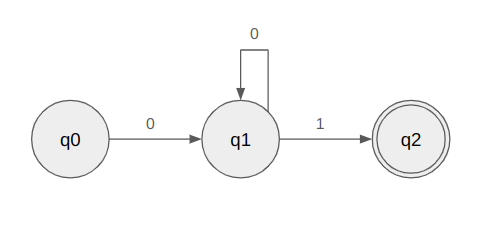
\includegraphics[width=0.9\textwidth]{images/pl/auto1.png}
    \caption{Autómata finito determinista para reconocimiento de la expresión regular $0^+1$.}
    \label{fig:PLAutomt}
\end{figure}

\subsection{Autómatas con pila}\label{subsection:automatPila}
Los autómatas con pila son cruciales para analizar gramáticas independientes del contexto, que generan lenguajes más complejos que los regulares. A diferencia de los autómatas finitos, estos autómatas poseen una pila para almacenar y recuperar información, lo que les permite manejar estructuras anidadas y dependencias a largo plazo.

Formalmente, un autómata con pila se define como una séptupla que incluye un conjunto de estados, un alfabeto de entrada, un alfabeto de pila, una función de transición, un estado inicial, un símbolo inicial de pila y un conjunto de estados finales. Existen versiones deterministas y no deterministas, siendo los deterministas aquellos que aceptan una cadena si, al finalizar su procesamiento, llegan a un estado final con la pila vacía. Esto garantiza que el autómata no solo reconozca la secuencia de símbolos de la entrada, sino que también cumpla con las estructuras de los lenguajes independientes del contexto.

\noindent
He aquí la escritura formal de un autómata con pila:
\begin{align*}
    M = (Q,A,B,\delta,q_0,Z_0,F)
\end{align*}

\noindent
donde:
\begin{itemize}
    \item $Q$ es un conjunto finito llamado \textbf{conjunto de estados}.
    \item $A$ es un alfabeto llamado \textbf{alfabeto de entrada}.
    \item $B$ es un alfabeto llamado \textbf{alfabeto de pila}.
    \item $\delta$ es una aplicación llamada \textbf{función de transición}.
    \item $q_0$ es un elemento de $Q$ llamado \textbf{estado inicial}.
    \item $Z_0 \in B$ es el \textbf{símbolo inicial de pila}
    \item $F$ es un subconjunto de $Q$, llamado \textbf{conjunto de estados finales}.
\end{itemize}

\section{Herramientas de procesamiento de lenguajes. Compiladores e intérpretes}\label{section:compiladores}
Lo acontecido en secciones anteriores en este capítulo ofrecen un marco teórico más que suficiente para el desarrollo de los siguientes capítulos que se centran en la parte práctica del proyecto. En esta última sección se hablará de herramientas prácticas para el procesamiento de lenguajes: los \textit{compiladores} e \textit{intérpretes}. Estas herramientas tienen como objetivo convertir el código fuente escrito en un lenguaje de programación a un formato que la máquina pueda ejecutar o interpretar directamente.

Un \textbf{compilador} es un programa que traduce código fuente escrito en lenguaje de alto nivel a lenguaje máquina o a un código intermedio. El proceso de compilación consta de varias fases:

\begin{enumerate}
    \item \textbf{Análisis léxico}: 
        \begin{itemize}
            \item El compilador lee el código fuente y lo descompone en tokens.
            \item Los tokens pueden ser identificadores, palabras clave, constantes, operadores, etc.
            \item Se simplifica y estructura el código fuente para las fases posteriores.
        \end{itemize}

    \item \textbf{Análisis sintáctico}:
        \begin{itemize}
            \item Organiza los tokens en un árbol sintáctico que representa la estructura gramatical.
            \item Verifica que la secuencia de tokens siga las reglas gramaticales del lenguaje.
            \item Identifica errores de sintaxis como paréntesis faltantes o errores en construcciones de bucles.
        \end{itemize}

    \item \textbf{Análisis semántico}:
        \begin{itemize}
            \item Verifica la corrección semántica del código, asegurando que los elementos del programa tengan sentido en su contexto.
            \item Incluye la verificación de tipos de datos y la coherencia en el uso de variables y funciones.
            \item Detecta errores como asignaciones de tipos de datos incorrectos o llamadas incorrectas a funciones.
        \end{itemize}

    \item \textbf{Generación de código intermedio}:
        \begin{itemize}
            \item Transforma el árbol sintáctico en una representación intermedia.
            \item Esta representación es independiente del lenguaje de programación y del hardware.
            \item Facilita la optimización del código y prepara la generación del código máquina.
        \end{itemize}

    \item \textbf{Optimización de código}:
        \begin{itemize}
            \item Mejora la representación intermedia para aumentar la eficiencia del programa.
            \item Incluye la eliminación de código inaccesible y la optimización de bucles.
            \item Esencial para mejorar el rendimiento y la eficiencia del código compilado.
        \end{itemize}

    \item \textbf{Generación de código máquina}:
        \begin{itemize}
            \item Convierte la representación intermedia en código de máquina ejecutable por el procesador.
            \item El código generado está optimizado para el hardware específico de destino.
            \item Completa el proceso de traducción resultando en un programa ejecutable o archivo objeto.
        \end{itemize}
\end{enumerate}


A diferencia de los compiladores, un \textbf{intérprete} no genera un archivo de salida ejecutable. En su lugar, leen y ejecutan el código fuente directamente, traduciendo el programa a medida que se ejecuta. Esto permite una mayor flexibilidad y una iteración más rápida durante el desarrollo, aunque puede tener un rendimiento más lento en comparación con los programas compilados. Los intérpretes también utilizan técnicas de análisis léxico y sintáctico para entender el código fuente, pero ejecutan las instrucciones inmediatamente después de su análisis.

También hay una variante que combina ambos enfoques, que es lo que se denomina como \textbf{compilador en tiempo de ejecución} (o \textit{Just-In-Time}). En la práctica en este proyecto, aunque se dispone de una fase de compilación que traduce código del lenguaje a código intermedio, su funcionamiento es más semejante al de un \textit{intérprete}, al traducir inmediatamente dichas instrucciones intermedias.

\begin{figure}[h]
    \centering
    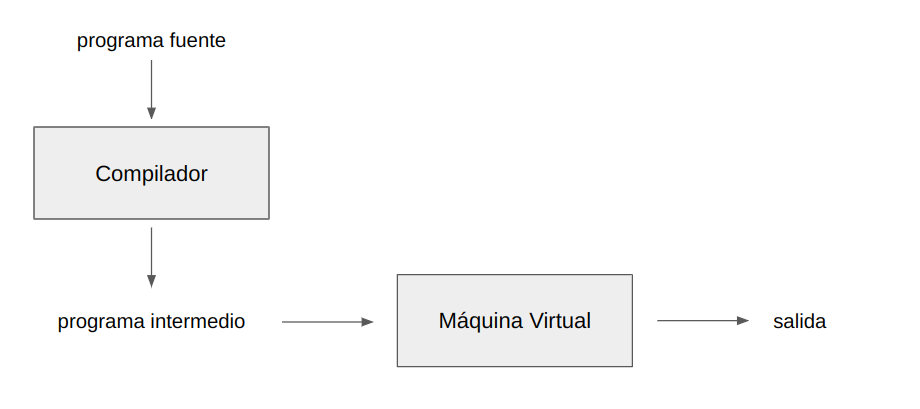
\includegraphics[width=1.0\textwidth]{images/pl/jit.png}
    \caption{Esquema de un compilador en tiempo de ejecución.}
    \label{fig:JITCompiler}
\end{figure}

        % Cuarta parte : Diseño e implementación del lenguaje Lamport
        \part{Diseño e implementación del lenguaje de programación Lamport}
        %\chapter{\textbf{Descripción del problema}}\label{chapter:problema}

Este trabajo busca responder a las dos siguientes preguntas: ¿cómo se puede optimizar, a nivel teórico y práctico, el estudio e implementación de los conceptos de diseño y desarrollo de programas concurrentes? ¿Qué métodos existen para verificar formalmente las propiedades de dichos programas? Aunque existen innumerables maneras de abordar estos desafíos planteados, sólo el uso de una metodología clara, segura y correcta resulta verdaderamente adecuado.

\section{Metodología: Desarrollo Ágil}
La siguiente frase de Siegbert Tarrasch, quien fue uno de los mejores jugadores de ajedrez de todos los tiempos, es digna de mención: \textit{"La belleza de un movimiento no se refleja sólo en su apariencia, sino en el pensamiento detrás de él"}. No basta con tener acciones o hechos; es esencial que detrás de ellos exista una \textbf{idea}, un \textbf{problema} o simplemente una \textbf{pregunta} que sirva de base para construir paso a paso todos los objetivos que se deseen alcanzar. Del mismo modo que en el ajedrez cada movimiento es estratégico y sigue una lógica o un plan, en un proyecto que precise de la ingeniería informática cada paso dado debe estar fundamentado y orientado hacia la resolución del problema central.

En un proyecto de ingeniería informática, es esencial identificar claramente el problema que se desea resolver y la razón subyacente. Una vez definido, es importante garantizar que el proyecto en cuestión realmente aborde dicho problema \cite{jj-agile-objetivos}. La estrategia más efectiva consiste en dividir el problema en segmentos más manejables, a los que podemos referirnos como \textit{objetivos}. La recurrente mención de la palabra \textbf{"problema"} subraya su importancia central en la metodología, pues no se espera otra cosa que \textit{solucionar dicho problema}.

El desarrollo ágil surgió tras la redacción y firma del \textit{Manifiesto por el Desarrollo Ágil de Software} \cite{agile-manifest} por diecisiete expertos en programación. Con el término \textit{ágil} no se alude únicamente a una metodología para el desarrollo de proyectos que precisan de rapidez y flexibilidad, sino también una filosofía que implica una forma distinta de trabajar y de organizarse a la que predominaba anteriormente, denominada \textit{metodología en cascada}. Así pues, por \textit{ágil} se entiende una mentalidad que se aplica a todo el ciclo de vida del desarrollo de software, centrada en el cliente y en la mejora continua de productos mínimamente viables cada vez más complejos \cite{jj-agile-manifesto}.

Todo proyecto debe nacer de una motivación inicial, respondiendo a interrogantes como \textit{``por qué''}, \textit{``para qué''}, \textit{``para quién''} y \textit{``cómo''}. Si bien todas estas cuestiones son importantes, la penúltima destaca particularmente porque el éxito radica en satisfacer los \textit{deseos} y \textit{necesidades} de un grupo específico de clientes o usuarios unidos por una característica común: un \textit{problema}. 
Resolverlo implica practicar la \textbf{empatía} con ellos, esforzándose por comprender profundamente sus necesidades y determinar cómo satisfacerlas de manera óptima, aportando \textbf{valor} con los recursos disponibles. Las entrevistas personales o el seguimiento de las tendencias actuales pueden proporcionar la perspectiva adecuada.

De ahí surgen las \textbf{Historias de Usuario}, que proporcionan una explicación informal desde el punto de vista del usuario final y siempre situadas dentro del dominio del problema, de una funcionalidad del software que principalmente tendrá que ver con la lógica de negocio del proyecto.\cite{jj-design-thinking}. Una vez definidas, lo que queda es especificar los productos que se entregarán a los clientes, descritos a través de una secuencia de \textbf{hitos} o \textbf{milestones}. La esencia del desarrollo ágil radica en efectuar mejoras iterativas sobre el producto, contando siempre con la aprobación del usuario. En consecuencia, el avance del proyecto no es lineal, sino un proceso incremental.

En resumen, el desarrollo ágil supuso un gran cambio en el paradigma de la organización y planificación de proyectos de ingeniería informática, colocando al usuario y sus necesidades en el centro del proceso, guiando cada paso a través de la empatía y una comprensión profunda del problema. Con herramientas como las Historias de Usuario y la propia naturaleza de la metodología basada en un proceso iterativo e incremental, se busca proporcionar soluciones más adaptadas y flexibles de la ingeniería moderna, puesto que las necesidades de los clientes pueden ir variando con el tiempo. Es un enfoque que valora la colaboración y la resiliencia, con el objetivo de siempre aportar valor, abordando así los actuales y futuros desafíos del mundo tecnológico.

\section{Clientes}
Tras haber explorado la esencia del desarrollo ágil y su prioridad hacia el usuario y sus deseos, ahora se profundizará en el concepto de \textbf{cliente}. Los problemas y expectativas de los clientes o usuarios son lo que impulsan las decisiones y acciones del equipo de desarrollo. 

Para identificar y comprender los distintos usuarios del compilador de código, se empleó una metodología centrada en las personas. Se llevaron a cabo entrevistas individuales a dos grupos de personas \textit{reales} \footnote{Aunque no es estrictamente necesario utilizar personas reales para el análisis de un problema en el desarrollo de un proyecto, hacerlo añade una dimensión \textit{humana} que, en mi experiencia con otros proyectos, aumenta considerablemente las probabilidades de éxito.} vinculadas a la asignatura de \textit{Sistemas Concurrentes y Distribuidos}: estudiantes y profesorado. A ambos grupos se les formuló una serie de preguntas, que se presentan a continuación.

\noindent
Las preguntas planteadas al alumnado de la asignatura fueron:
\begin{itemize}
    \item \textit{¿Te resulta complicado entender los conceptos o fundamentos teóricos de la asignatura?}
    \item \textit{¿Eres capaz de resolver un problema que involucre concurrencia sin programarlo explícitamente?}
    \item \textit{¿Notas una diferencia significativa entre la teoría y práctica de la asignatura?}
    \item \textit{¿Crees que programar en el pseudocódigo específico de la asignatura te facilitaría su aprendizaje?}
\end{itemize}

\noindent
Las preguntas planteadas al profesorado fueron:
\begin{itemize}
    \item \textit{¿Consideras que la asignatura es difícil para los estudiantes?}
    \item \textit{¿Ves una diferencia significativa entre la teoría y la práctica de la asignatura?}
    \item \textit{¿Piensas que programar en el pseudocódigo específico de la asignatura ayudaría a los alumnos durante el curso? ¿Facilitaría tu labor docente al explicar los conceptos?}
\end{itemize}

Las dos últimas preguntas de cada grupo son similares, buscando comprobar la concordancia entre ambos puntos de vista. Las respuestas de los estudiantes indican que, aunque la asignatura posee una complejidad relativa en comparación con otras del grado, los conceptos en sí no son difíciles de asimilar. La verdadera barrera surge al aplicar estos conceptos en el diseño de sistemas concurrentes o al tratar de resolver problemas sin recurrir a un lenguaje de alto nivel, como C++. Los estudiantes generalmente consideran que se desenvuelven mejor en la práctica que en la teoría. Esta preferencia puede deberse a su familiaridad con el enfoque práctico adoptado en los primeros años del grado, con este lenguaje en particular. Por tanto, la respuesta a la última pregunta suele ser un \textit{sí} rotundo.

El profesorado, por su parte, no ve a su asignatura como particularmente complicada y no percibe una gran diferencia entre la teoría y práctica. Sin embargo, muestran empatía hacia los estudiantes, entendiendo que ellos puedan sentir una mayor complejidad. Coinciden en que disponer de un lenguaje de programación con la sintaxis propuesta en la asignatura podría facilitar una enseñanza más didáctica y accesible.

Con esta información no sólo obtenemos la motivación mencionada en la sección anterior, sino que también podemos identificar a los dos usuarios potenciales del compilador a desarrollar. A continuación, se describirá detalladamente el perfil de cada tipo de usuario.

\subsection{Tipo de usuario 1: Estudiante}
Se proporciona una descripción detallada de un perfil de usuario de tipo estudiante:

\begin{description}
    \item[Nombre:] Luis Martínez
    \item[Características Demográficas:] \hfill
        \begin{itemize}
            \item Edad: 19 años.
            \item Estudiante universitario de ingeniería informática, actualmente cursando la asignatura de \textit{Sistemas Concurrentes y Distribuidos}.
        \end{itemize}
    \item[Necesidades y Objetivos:] Luis aspira a aprobar la asignatura de \textit{Sistemas Concurrentes y Distribuidos} para avanzar en sus estudios. Además, busca comprender conceptos que sean importantes en futuras asignaturas relacionadas con su grado.
    
    \item[Habilidades Técnicas:] Posee habilidades de programación de nivel principiante a intermedio. Es probable que esta sea su primera experiencia con la implementación de programas no secuenciales.
    
    \item[Escenarios de Uso Comunes:] Luis utiliza el compilador para validar ejercicios específicos de la clase sobre sincronización de hebras o procesos.
    
    \item[Limitaciones:] Aunque Luis se siente cómodo programando en lenguajes de alto nivel como C++, enfrenta dificultades al comprender la sintaxis del pseudocódigo. Esto puede dificultar su capacidad para traducir rápidamente los conceptos teóricos en implementaciones prácticas utilizando pseudocódigo.
    
    \item[Expectativas:] Espera poder disponer de un lenguaje de pseudocódigo funcional, pudiendo añadir comentarios explicativos a cada línea de código para facilitar su comprensión. Además, desea que las ejecuciones de los programas se visualicen de forma clara, permitiéndole seguir el proceso paso a paso para consolidar su entendimiento de los conceptos teóricos.
\end{description}

\subsection{Tipo de usuario 2: Profesor}
Se proporciona una descripción detallada de un posible perfil de usuario de tipo profesor:

\begin{description}
    \item[Nombre:] Laura Ruiz
    \item[Características Demográficas:] \hfill
        \begin{itemize}
            \item Edad: 42 años.
            \item Profesora titular de la asignatura \textit{Sistemas Concurrentes y Distribuidos} en la facultad de Ingeniería Informática.
            \item Más de 10 años de experiencia docente en el campo de la informática.
        \end{itemize}
    \item[Necesidades y Objetivos:] Desea que sus estudiantes comprendan a fondo los conceptos y aplicaciones de los sistemas concurrentes y distribuidos. Busca herramientas y métodos que puedan hacer que la enseñanza sea más interactiva y efectiva.
    
    \item[Habilidades Técnicas:] Amplios conocimientos en programación, sistemas concurrentes, y pedagogía. Familiarizada con varios lenguajes de programación, incluido C++.
    
    \item[Escenarios de Uso Comunes:] Utilizar el compilador para demostrar ejemplos en clase, proponer ejercicios prácticos a los estudiantes y evaluar soluciones propuestas por ellos. Puede usarlo también para simular escenarios concurrentes y mostrar visualmente a los estudiantes cómo funcionan.
    
    \item[Limitaciones:] Prefiere que la herramienta tenga una interfaz amigable y sea intuitiva, ya que no desea invertir mucho tiempo en aprender a usarla. 
    
    \item[Expectativas:] Espera que el compilador permita explicaciones paso a paso y que pueda integrarse fácilmente con otros recursos didácticos. Le interesa que el pseudocódigo esté alineado con el contenido teórico de la asignatura, facilitando la transición entre teoría y práctica.
\end{description}

\newpage

\section{Historias de Usuario}

A través de las \textbf{Historias de Usuario}, se busca no solo definir qué es lo que el software debe hacer, sino también por qué es relevante hacerlo y cuál es el valor que se ofrece al usuario final. A continuación, se presentarán las Historias de Usuario identificadas para el desarrollo del compilador de código y cómo estas sientan las bases para los \textit{milestones} y Productos Mínimamente Viables del proyecto.

\begin{itemize}
    \item \textbf{Historia de usuario 1 (HU1):} Como estudiante de la asignatura, Luis quiere disponer de un compilador para escribir y ejecutar programas en el lenguaje de pseudocódigo propuesto en las transparencias, con el objetivo de practicar y verificar el funcionamiento de las soluciones a los ejercicios planteados.
    \item \textbf{Historia de usuario 2 (HU2):} Como profesora de la asignatura, Laura quiere contar con un compilador del lenguaje de las transparencias para poder explicar de forma más práctica los conceptos teóricos sin requerir un lenguaje de programación estándar como puede ser C++ o Java, además de poder revisar y analizar el código fuente desarrollado eventualmente por sus alumnos, y proporcionarles retroalimentación personalizada a los mismos.
\end{itemize}

\section{Milestones del proyecto: Productos Mínimamente Viables (PMV)}

Siguiendo la línea de las \textit{Historias de Usuario} y la importancia de establecer una comunicación efectiva con el usuario final, es el momento de definir productos entregables concretos que materialicen estas historias en el transcurso del desarrollo, que comúnmente se denomina \textbf{Productos Mínimamente Viables (PMV)}. Están diseñados no solo como representaciones tangibles del progreso, sino también como puntos de revisión donde se puede evaluar y adaptar el proyecto basándose en la retroalimentación aportada o por el propio cliente o por otro equipo de desarrollo. Los \textbf{milestones} o \textbf{hitos} sirven para secuenciar y organizar estos PMV en el ámbito del desarrollo ágil. A continuación, se enumeran los \textit{milestones} establecidos para este proyecto y cómo cada uno aporta al objetivo final del compilador de código.

\subsection{Milestone 0: Infraestructura del proyecto y definición del lenguaje.}\label{subsection:PMV0}
El primer hito del proyecto se centra en establecer una base sólida para su desarrollo. Comienza con una definición clara del problema, obtenida a través de entrevistas con usuarios potenciales, y la formulación detallada de este problema junto con la elaboración de las historias de usuario. Paralelamente, se lleva a cabo un estudio exhaustivo del lenguaje de pseudocódigo utilizado en la asignatura de Sistemas Concurrentes y Distribuidos, analizando sus componentes y definiendo su gramática utilizando la notación de Backus-Naur. En el aspecto técnico, se seleccionan cuidadosamente herramientas esenciales para el proyecto, incluyendo el lenguaje de programación para el compilador, un sistema de control de versiones, gestores de dependencias y tareas, herramientas de linting y ejecución de tests. Además, se configuran estas herramientas para garantizar la gestión eficiente de las dependencias, la calidad del código, y la automatización de tareas repetitivas como la compilación y la ejecución de tests.

\subsection{Milestone 1: Implementación del Analizador Léxico.}\label{subsection:PMV1}
Este hito se dedica a la construcción y validación del analizador léxico, una etapa crucial en el proceso de interpretación de cualquier lenguaje de programación. El foco principal es desarrollar una herramienta capaz de convertir una cadena de entrada en una serie de tokens identificables, que serán fundamentales para las etapas posteriores del compilador. Para lograrlo, se considera una herramienta generadora de analizadores léxicos que se ajuste a las especificaciones del lenguaje y las necesidades del proyecto. A continuación, se definen los tokens del lenguaje, incluyendo palabras reservadas, identificadores y operadores, junto con sus patrones de reconocimiento. La implementación del analizador léxico se realiza utilizando esta herramienta, asegurando su capacidad para reconocer y clasificar correctamente cada token. Además, se establece una tarea de generación del analizador léxico para facilitar su integración con el sistema, así como una tarea de limpieza de código objeto y ficheros compilados para mantener la organización y eficiencia del proyecto.

\subsection{Milestone 2: Implementación del Analizador Sintáctico.}\label{subsection:PMV2}
El segundo hito se enfoca en el diseño e implementación del analizador sintáctico, esencial para verificar la estructura correcta del código fuente en el lenguaje de pseudocódigo, según la gramática definida previamente. Este proceso incluye la definición de operadores, su aridad, asociatividad y orden de precedencia. Se selecciona una herramienta generadora de analizadores sintácticos y se ajusta la gramática del lenguaje. Tras implementar el analizador, se establece una estrategia para la recuperación de errores sintácticos y se define una tarea para su generación/compilación. Paralelamente, se desarrolla el Árbol Sintáctico Abstracto (AST), integrándolo con el analizador y definiendo una módulo para su gestión. Se implementan estructuras y funciones para la gestión de errores sintácticos y su integración con el analizador. Además, se llevan a cabo pruebas de integración y se desarrolla el programa principal del compilador, permitiendo la lectura de ficheros de texto plano, el procesamiento del pseudocódigo, la impresión del AST o los errores sintácticos detectados.

\subsection{Milestone 3: Implementación del Analizador Semántico.}\label{subsection:PMV3}
Este milestone se enfoca en el diseño e implementación del analizador semántico, una fase crítica que garantiza que el código fuente en el lenguaje de pseudocódigo no solo esté estructuralmente correcto (como asegura el analizador sintáctico) sino que también posea un significado lógico y coherente. El proceso incluye la descripción semántica del lenguaje y la implementación de una Tabla de Símbolos para gestionar identificadores y sus propiedades. Se desarrollan algoritmos clave para la resolución de nombres y la comprobación de tipos, asegurando que cada identificador se declare correctamente y que las operaciones entre diferentes tipos de variables sean válidas. Se establece una tarea de compilación para el módulo Analizador Semántico, facilitando su integración con otros componentes del compilador. Además, se realizan pruebas de integración para validar su funcionamiento en diversos escenarios de código. Se implementan estructuras y funciones para la gestión y reporte de errores semánticos, integrando el módulo de errores con el analizador para proporcionar retroalimentación específica al usuario. Finalmente, se habilita la función de análisis semántico dentro del flujo del compilador, proporcionando mensajes claros sobre el éxito del análisis o los errores detectados.

\subsection{Milestone 4: Análisis e implementación de la fase de generación de código intermedio.}\label{subsection:PMV4}
El cuarto hito se centra en el diseño e implementación de la fase de generación de código intermedio, un proceso clave que convierte el árbol de análisis sintáctico en una representación intermedia más cercana al código de máquina. Esta fase comienza con la selección de una representación intermedia adecuada para el lenguaje desarrollado y la definición de sus instrucciones, especificando operandos y usos. Se desarrolla un generador de código intermedio, con tablas para mapear variables, etiquetas y literales, y controladores para la generación y optimización del código. Paralelamente, se implementa un manejador de registros de eventos para documentar y ofrecer transparencia sobre las fases de análisis del compilador, incluyendo el análisis sintáctico, semántico y la generación del código intermedio. Se llevan a cabo pruebas de integración para asegurar la funcionalidad del módulo de generación de código intermedio y se habilita su función dentro del flujo general del compilador, junto con la generación de ficheros de registro de eventos para las distintas fases de análisis.


\subsection{Milestone 5: Análisis e implementación del compilador de código intermedio o máquina virtual}\label{subsection:PMV5}
El quinto hito del proyecto se centra en el diseño e implementación de un compilador para el código intermedio generado en las fases anteriores, que actúa como una máquina virtual. Esta máquina virtual está diseñada para ejecutar la representación intermedia, creando un entorno controlado que simula las operaciones de una máquina real de forma abstracta y agnóstica a la arquitectura del hardware. Para lograrlo, se implementan varios componentes clave: un esquema de traducción de direcciones virtuales a físicas, una abstracción de bloque de memoria, la memoria de la máquina virtual, un vector de registros de CPU, la CPU de la máquina virtual y un sistema operativo simulado para la máquina. Además, se aborda el tratamiento de excepciones como ZeroDivision e IndexOutOfBounds. La finalización de este milestone incluye realizar pruebas de integración exhaustivas para asegurar la funcionalidad y la integración adecuada de la máquina virtual con el resto del sistema.

\subsection{Milestone 6: Desarrollo teórico. Fundamentos matemáticos y tecnológicos}\label{subsection:PMV6}
El sexto milestone se enfoca en el desarrollo teórico, introduciendo los conceptos fundamentales de los sistemas concurrentes y distribuidos y realizando un estudio detallado de las lógicas formales, con énfasis en la Lógica Temporal de Acciones. Este enfoque teórico está diseñado para proporcionar una comprensión profunda de las bases matemáticas y lógicas necesarias para la verificación formal de sistemas concurrentes. Se explora la Lógica Temporal de Acciones, desarrollada por Leslie Lamport, para entender cómo se puede aplicar en el contexto de la verificación y el aseguramiento de la confiabilidad y coherencia en los sistemas concurrentes. El estudio se extiende a la explicación de cómo estos principios teóricos se integran y aplican en la práctica, resaltando su relevancia en el diseño, análisis y evaluación de sistemas que requieren una sincronización y coordinación efectivas. Este milestone no solo fortalece la base teórica del proyecto, sino que también proporciona a los usuarios las herramientas y conocimientos necesarios para abordar desafíos complejos en el campo de los sistemas concurrentes y distribuidos, preparándolos para enfrentar y resolver problemas prácticos con una sólida comprensión teórica.


        %\chapter{\textbf{Estado del arte}}
La \textit{programación concurrente} sienta sus bases en la década de los 1960 con la aparición de los sistemas operativos multiprogramación, que pretendían resolver uno de los problemas más críticos que se daban en aquella época: el uso eficiente de los recursos hardware. Anteriormente, la CPU ejecutaba sólo un programa a la vez, quedando inactiva si se producían operaciones de entrada/salida subutilizando sus recursos, produciendo como resultado un rendimiento deficiente. Con la multiprogramación, varios programas podían residir simultáneamente en la memoria principal, permitiendo a la CPU ejecutar otro programa diferente mientras se gestionaba una interrupción de E/S. Esta gestión se facilitó gracias a la invención de los ``canales'', controladores de dispositivos que operaban de forma independiente. Esta revolucionaria técnica tuvo un gran impacto en algunos sistemas informáticos que se desarrollaban por aquel entonces, como es el caso de los ``mainframes'' \cite{TecnologiaInformaticaMainframe}.


La programación concurrente fue inicialmente motivo de preocupación de los diseñadores de sistemas operativos. Al final de esta década de 1960, los diseñadores de hardware desarrollaron máquinas multiprocesador, que supusieron todo un reto para la implementación de nuevos sistemas operativos adaptados a estos recursos, pero también definió una nueva oportunidad para que los desarrolladores de aplicaciones pudieran emerger y posicionarse en el mercado laboral como una profesión con grandes expectativas a futuro.



El primer gran reto de esta nueva técnica de programación fue resolver lo que se denomina como: \textit{el problema de la sección crítica} \cite{GeeksForGeeksCriticalSection}. Este desafío central se refiere al desarrollo de algoritmos efectivos para la sincronización de procesos concurrentes que requieren acceder a un recurso compartido. La importancia de resolver este problema radica en la necesidad de evitar conflictos y garantizar la coherencia de los datos cuando múltiples procesos intentan leer o modificar el mismo recurso simultáneamente. La correcta gestión de la sección crítica es crucial para asegurar que los sistemas concurrentes funcionen de manera fiable y eficiente. Para entender mejor y modelar este reto, se plantearon problemas teóricos como \textit{la cena de los filósofos} \cite{brosgol1996dining}, \textit{lectores y escritores} \cite{nithyasrikannathalreaders}, \textit{el barbero durmiente} \cite{SariSleepingBarber} o el \textit{problema de los fumadores} \cite{MTUSmokerProblem}.


Estos escenarios anteriormente mencionados han sido ampliamente estudiados, generando miles de artículos que proponen soluciones, mejoras, debates y nuevas implementaciones de primitivas de sincronización como los semáforos o los monitores, que simplificaban la tarea del programador. Paralelamente, los lenguajes de programación de alto nivel estaban proliferando y evolucionando. Un ejemplo notable es Simula \cite{Sklenar1997OOPSimula}, desarrollado en la década de 1960 por Ole-Johan Dahl y Kristen Nygaard. Considerado uno de los primeros lenguajes orientados a objetos, Simula también introdujo conceptos fundamentales que influirían en la simulación de concurrencia, aunque su principal aporte fue establecer las bases para la programación orientada a objetos, un paradigma que tendría un impacto significativo en el desarrollo futuro de lenguajes y técnicas de programación concurrente.


Al final de la década de 1970 y principios de 1980, el surgimiento de redes de ordenadores como ARPANET, que facilitó la computación en áreas amplias, y el desarrollo de tecnologías como Ethernet para redes locales, marcó el comienzo de una nueva era en la informática. Estos avances no solo transformaron la forma en que las computadoras se conectaban y comunicaban entre sí, sino que también ampliaron significativamente el campo de la programación concurrente. Mientras la programación concurrente se enfoca en gestionar múltiples procesos dentro de un mismo sistema, las redes de computadoras introdujeron el desafío de coordinar procesos que se ejecutan en diferentes máquinas físicas. Esto dio origen a lo que se conoce como \textit{programación distribuida}, un enfoque que extendía los principios de la programación concurrente a sistemas distribuidos cuya esencia reside en que los procesos interactúan entre ellos a través del envío de mensajes en vez de escribir y leer variables compartidas.


A medida que la programación concurrente y distribuida ganaban relevancia en la década de 1980 y 1990, su integración en los lenguajes de programación de alto nivel comenzó a materializarse de manera significativa. Un hito notable en este desarrollo fue el lenguaje de programación Ada \cite{burns1998concurrency}, introducido en 1983. Diseñado originalmente para satisfacer las exigentes necesidades de los proyectos de defensa y sistemas en tiempo real, Ada se destacó por su soporte nativo para la programación concurrente. Su enfoque en la seguridad, la fiabilidad y la gestión sofisticada de tareas concurrentes lo convirtió en una herramienta fundamental para aplicaciones críticas. Posteriormente, en la década de 1990, Java emergió como un lenguaje de programación influyente, llevando la programación concurrente a un público más amplio. Con su API de concurrencia, Java simplificó la gestión de hilos y procesos concurrentes, haciendo que la programación de este tipo fuera más accesible y manejable para los desarrolladores. Esta API proporcionó un conjunto robusto de herramientas y estructuras para el manejo eficiente de tareas concurrentes y sistemas distribuidos, reflejando la creciente demanda de aplicaciones que operaban en entornos de red y web. La evolución de la programación concurrente en Ada y Java no solo demuestra cómo se han adaptado los lenguajes de programación a desafíos técnicos complejos, sino también cómo han evolucionado para satisfacer las necesidades de aplicaciones modernas en diversos entornos de computación. Pero no solo los lenguajes en sí, sino también las herramientas para crearlos, evolucionaron significativamente durante este periodo. El desarrollo de herramientas avanzadas para generar compiladores facilitó la creación de lenguajes de programación más sofisticados, especialmente aquellos diseñados para la programación concurrente y distribuida. Estas herramientas permitieron a los diseñadores de lenguajes experimentar con nuevas construcciones y paradigmas, facilitando el desarrollo de lenguajes que pudieran manejar de manera más eficiente y segura las complejidades inherentes a la concurrencia y la distribución. 


Sin embargo, cada vez que se implementaban mejoras en la programación concurrente y distribuida, con nuevas ideas y hardware, la complejidad de los programas aumentaba exponencialmente. Esto llevó a un incremento similar en la dificultad de verificar su funcionamiento correcto. Poco después del origen de este modelo de programación, surgió la necesidad de introducir formalismos capaces de demostrar rigurosamente que un programa concurrente posee ciertas propiedades. En este contexto, las herramientas matemáticas formales, especialmente la lógica temporal, se convirtieron en indispensables. La lógica temporal, que se ocupa de los aspectos temporales del razonamiento en la lógica matemática, permitía especificar y razonar sobre el comportamiento de los programas a lo largo del tiempo, asegurando propiedades como la seguridad (nunca ocurrirá nada malo) y la vivacidad (realmente sucede algo bueno) en sistemas concurrentes.


Un desarrollo particularmente significativo en el campo de la verificación de sistemas fue la Lógica Temporal de Acciones (TLA) de Leslie Lamport, cuya vida y carrera han sido tan influyentes como sus logros académicos \footnote{Lamport fue también el desarrollador inicial de \LaTeX, el sistema de composición de documentos utilizado para redactar este informe. A lo largo de su carrera, ha sido galardonado con numerosos premios, incluyendo el prestigioso Premio Turing, por sus contribuciones a la informática teórica. Sus trabajos, incluyendo la TLA, han influenciado tanto la teoría como la práctica en el diseño y verificación de sistemas distribuidos y concurrentes.}. Nacido en 1941 en Nueva York, Lamport demostró un interés temprano en las matemáticas y la ciencia, lo que eventualmente lo llevó a obtener un Ph.D. en Matemáticas. Su transición hacia la computación fue motivada por un interés creciente en los problemas de sistemas distribuidos y la sincronización de procesos, un campo en el que se convertiría en un líder mundial.


Lamport, una figura destacada en la computación teórica, ha sido pionero en proponer metodologías rigurosas para el diseño y análisis de algoritmos en entornos complejos. La metodología de la TLA, que permite describir el comportamiento de un sistema en términos de estados y transiciones entre estos, facilita la verificación de propiedades críticas de sistemas complejos. Su visión era proporcionar una herramienta que no solo facilitara la especificación precisa de estos sistemas, sino que también permitiera su análisis y verificación de manera sistemática y confiable.


En la actualidad, la programación concurrente y distribuida se ha consolidado como un pilar fundamental en el panorama tecnológico. En el ámbito de la computación ubicua, donde múltiples dispositivos y sensores interactúan en tiempo real, es crucial mantener la precisión y la sincronización para ofrecer experiencias de usuario cohesivas y confiables. En el campo de la inteligencia artificial, la capacidad de manejar operaciones de procesamiento paralelo y distribuido resulta esencial para analizar grandes conjuntos de datos y ejecutar complejos algoritmos de aprendizaje automático. La corrección y eficiencia de los procesos concurrentes son vitales en áreas como el reconocimiento de patrones y el procesamiento de lenguaje natural. En el procesamiento multimedia, esta programación facilita la manipulación eficiente de contenidos de alta definición en tiempo real, siendo la precisión en la sincronización y la integridad de los datos fundamentales en aplicaciones que van desde la edición de vídeo hasta la transmisión en vivo. Estos ejemplos ilustran la omnipresencia y el impacto crucial de la programación concurrente y distribuida en la tecnología moderna, resaltando la necesidad de métodos rigurosos para su verificación fiable, lo que a su vez impulsa la innovación tecnológica.
        %\chapter{Planificación}

\section{Metodología utilizada}


\section{Temporización}

\section{Seguimiento del desarrollo}

        \chapter{\textbf{Infraestructura tecnológica}}
Tras haber definido en el capítulo ~\ref{chapter:problema} el problema que aborda este proyecto y la motivación que lo impulsa, es clave considerar un aspecto clave en el desarrollo de cualquier iniciativa tecnológica: \textit{las herramientas utilizadas}. Mientras que las preguntas \textit{¿qué?}, \textit{¿por qué?}, \textit{¿para quién?} y \textit{¿cómo?} han guiado la formulación y la estructuración del proyecto, la pregunta \textit{¿con qué?} se centra en los recursos y tecnologías que hacen posible su realización. Este capítulo se dedica a explorar las diversas herramientas y plataformas seleccionadas para el desarrollo del compilador del lenguaje Lamport, detallando cómo cada una contribuye a las distintas facetas del proyecto.

\section{Licencia del Proyecto: GPL v3.0}
La licencia escogida para este proyecto es la \textit{General Public License versión 3.0} (GPL v3.0) \cite{gplv3}, una de las licencias de software libre más populares y respetadas. Esta licencia es fundamental para definir las condiciones de uso, modificación y distribución del software desarrollado. La GPL v3.0 es conocida por promover la libertad de uso y la colaboración abierta, al tiempo que protege los derechos de autor. Sus características clave incluyen:

\begin{itemize}
    \item \textbf{Libertad para ejecutar el programa}: Los usuarios tienen libertad para ejecutar el software para cualquier propósito.
    \item \textbf{Libertad para estudiar y modificar el programa}: El acceso al código fuente permite a los usuarios estudiar cómo funciona el programa y adaptarlo a sus necesidades.
    \item \textbf{Libertad para redistribuir copias}: Los usuarios pueden copiar y distribuir el software en su forma original.
    \item \textbf{Libertad para distribuir versiones modificadas}: Los usuarios pueden modificar el software y distribuir sus propias versiones, lo que fomenta la innovación y la mejora continua.
    \item \textbf{Protección de derechos}: La licencia asegura que el software permanezca libre y que cualquier trabajo derivado también esté protegido bajo los mismos términos.
\end{itemize}

\section{GitHub: Plataforma de Control de Versiones y Colaboración}
GitHub, basado en la herramienta de control de versiones Git, es mucho más que un simple repositorio de código fuente. Es una de las plataformas de control de versiones y colaboración más grandes y populares del mundo, albergando millones de proyectos.

Esta plataforma integral no solo facilita la gestión de versiones de código, sino que también potencia el trabajo colaborativo y la administración de proyectos mediante una variedad de herramientas y funcionalidades. Estas incluyen:

\begin{itemize}
    \item \textbf{Issues}: Esenciales para destacar problemas o tareas dentro del repositorio, permitiendo un seguimiento organizado y asignación de responsabilidades a los miembros del equipo.
    \item \textbf{Integración continua}: Práctica fundamental en el desarrollo moderno, que integra y prueba automáticamente el código a medida que se desarrolla, facilitada por herramientas como GitHub Actions.
    \item \textbf{Ramas y Pull Requests}: Permiten el desarrollo paralelo de características o pruebas y la propuesta de cambios al código principal, posibilitando una revisión y colaboración detallada en cada cambio propuesto.
\end{itemize}

\section{Lenguajes de programación: C y C++}
Puesto que el problema descrito se resuelve \textit{desarrollando código}, es natural decidir antes de empezar en qué lenguaje se va a dar solución a las historias de usuario mencionadas.


Los lenguajes C y C++ son elecciones prominentes cuando se busca eficiencia y rendimiento en un sistema. Estos lenguajes ofrecen un control cercano al hardware, permitiendo optimizaciones a nivel de memoria y ejecución. Además, la naturaleza compilada de sendos lenguajes asegura que el código se ejecuta directamente en la máquina anfitriona sin la necesidad de un intérprete intermedio, garantizando tiempos de respuesta rápidos. El compilador, al requerir análisis y ejecución eficiente del código fuente, se beneficia significativamente de estas características. Adicionalmente, la extensa biblioteca estándar y la amplia disponibilidad de bibliotecas de terceros en ambos lenguajes facilitan la implementación de funcionalidades complejas. Por estas razones, la decisión de utilizar C y C++ para definir el compilador garantiza un balance óptimo entre rendimiento y flexibilidad.

\section{Gestor de tareas y dependencias: Make}
Make es una herramienta de construcción automatizada que permite a los desarrolladores definir tareas y las dependencias entre ellas. Se utiliza ampliamente en programación para automatizar la compilación, pruebas, y otras tareas relacionadas con el ciclo de vida del software. Un archivo denominado `Makefile` contiene un conjunto de directivas y reglas que especifican cómo derivar los archivos objetivo a partir de archivos fuente. Al ejecutar la orden `make`, la herramienta lee el archivo `Makefile`, evalúa las dependencias y ejecuta las reglas necesarias en el orden adecuado.


\noindent
En este proyecto se usará para las siguientes tareas:
\begin{itemize}
    \item Gestión de las dependencias del proyecto. El Makefile debe contener reglas que permitan instalar, desinstalar y comprobar la versión de las dependencias del compilador.
    \item Compilación del compilador. Debe contener las reglas para generar código objeto de todos los módulos implementados y compilarlos en un único ejecutable binario final.
\end{itemize}

\section{Análisis y Depuración de Memoria: Valgrind}
Valgrind es una herramienta de programación para la detección de errores en memoria y análisis de rendimiento. Permite a los desarrolladores identificar problemas relacionados con la gestión de memoria, como fugas de memoria y acceso a punteros no válidos, entre otros problemas comunes en C y C++. Al ejecutar programas bajo el control de Valgrind, se pueden detectar estos problemas en tiempo real, lo que facilita la identificación y corrección de errores en las etapas tempranas del desarrollo.

\section{Contenedores virtuales: Docker}
Docker es una plataforma de que permite a los desarrolladores empaquetar aplicaciones y sus dependencias en contenedores. Estos contenedores pueden ser ejecutados de manera consistente en cualquier entorno que tenga Docker instalado, independientemente de las diferencias en ese entorno con respecto al entorno original donde se desarrolló la aplicación. En generación de contenedores, a diferencia de la virtualización tradicional, no se crea una máquina virtual completa para cada aplicación, sino que comparte el mismo núcleo del sistema operativo y aísla la aplicación en un contenedor. Esto hace que Docker sea más ligero, más rápido y más eficiente en términos de recursos que las máquinas virtuales tradicionales.


En este proyecto se utilizará para aislar el compilador del lenguaje en un entorno donde ya disponga de todas las dependencias necesarias para funcionar, aprovechando todas las ventajas anteriormente mencionadas.

\section{Generación de analizadores léxicos: Flex}
La generación de analizadores léxicos es un imprescindible en el análisis de lenguajes de programación, donde las expresiones regulares y los autómatas juegan un papel importantísimo. Estos analizadores, diseñados para reconocer patrones léxicos en el código fuente, son a menudo construidos utilizando herramientas como Flex, que convierte expresiones regulares en autómatas finitos. Flex simplifica este proceso al permitir la definición de patrones léxicos a través de expresiones regulares, que luego son automáticamente transformadas en un AFND y posteriormente en un AFD para el análisis eficiente del texto de entrada. Este enfoque aprovecha la teoría de autómatas y las propiedades de las expresiones regulares para crear sistemas capaces de descomponer y entender la estructura léxica de los lenguajes de programación.


\section{Generación de analizadores sintácticos: Bison}
La utilidad de los autómatas con pila se extiende más allá de la teoría y encuentra una aplicación práctica significativa en la generación de analizadores sintácticos. El proceso de análisis sintáctico implica reconocer patrones y estructuras sintácticas más complejas, una tarea para la cual los autómatas con pila están especialmente equipados. Gracias a su capacidad de almacenar y manejar información contextual en la pila, pueden eficientemente analizar gramáticas independientes del contexto, que son típicas en la mayoría de los lenguajes de programación modernos.

Herramientas como Bison, utilizan la teoría de los autómatas con pila para generar analizadores sintácticos. Estas herramientas toman una especificación de gramática y producen un analizador que puede descomponer y analizar estructuras lingüísticas complejas, siguiendo las reglas definidas en la gramática. Al igual que con los analizadores léxicos, el uso de autómatas con pila simplifica enormemente el proceso de desarrollo de software, permitiendo a los programadores y desarrolladores de lenguajes centrarse en la definición de reglas gramaticales, mientras la herramienta maneja los detalles del análisis sintáctico.

\subsection{Gramáticas LALR(1) y su Aplicación en Bison}
Las gramáticas LALR(1), o "Look-Ahead LR(1)", son un tipo de gramática utilizada en la generación de analizadores sintácticos, especialmente en herramientas como Bison. Estas gramáticas son una variante de las gramáticas LR(1), que son un tipo de gramática independiente del contexto.

La característica distintiva de las gramáticas LALR(1) es su capacidad para considerar un ``look-ahead'' de un símbolo al tomar decisiones de análisis. Esto significa que el analizador revisa el símbolo actual y el siguiente para determinar la acción a realizar. Este enfoque ayuda a manejar conflictos de análisis que podrían surgir en gramáticas más simples.

Bison utiliza gramáticas LALR(1) debido a su eficiencia en el manejo de la mayoría de las construcciones de lenguajes de programación, mientras que mantiene un equilibrio entre la complejidad del analizador y su capacidad para manejar gramáticas amplias. Al emplear LALR(1), Bison es capaz de generar analizadores eficientes y potentes que pueden procesar gramáticas complejas con un buen rendimiento y precisión.
	\chapter{\textbf{Estudio y diseño del lenguaje Lamport}}\label{chapter:lamportDesign}
El lenguaje \textit{Lamport}, nombrado en honor al renombrado informático Leslie Lamport, emerge como una herramienta didáctica y a la vez completamente funcional. Su propósito es modelar, diseñar y simular sistemas concurrentes y distribuidos.

En este capítulo, se llevará a cabo un estudio detallado sobre el pseudocódigo propuesto en la asignatura \textit{Sistemas Concurrentes y Distribuidos}, que sustentará la base del lenguaje destino \textit{Lamport}. Se discutirán sus objetivos de diseño, principales características y cómo estas contribuyen a abordar los desafíos de modelar y simular sistemas concurrentes. Se profundizará en aspectos como la sintaxis, semántica y otras características esenciales. Finalmente, se presentará una definición formal de la gramática del lenguaje Lamport, orientada a ser un recurso valioso para quienes aspiren a aprender o instruir sobre sistemas concurrentes, e incluso utilizarlo como un lenguaje de programación más.

\section{Análisis del pseudocódigo base}\label{sec:pseudoAnalisis}
El pseudocódigo, una representación abstracta y simplificada de la lógica de programación, es un elemento crucial en la fase de diseño de sistemas informáticos. En la asignatura \textit{Sistemas Concurrentes y Distribuidos} \cite{capel2020sistemas}, se propone un pseudocódigo específico que sienta las bases para la concepción del lenguaje \textit{Lamport}. Analizar este pseudocódigo nos permite entender su estructura, características y potenciales áreas de mejora o adaptación.

A continuación se presentarán una serie de ejemplos representativos del pseudocódigo, ilustrando sus principales componentes. Posteriormente, se desglosarán sus elementos fundamentales y se considerará su relación con lenguajes de programación más convencionales, permitiendo así contextualizar su diseño y utilidad.

\newpage

\subsection{Ejemplos de pseudocódigo}\label{subsec:pseudoAnalisisEjemplos}

Los ejemplos que se presentan a continuación ofrecen una vista panorámica sobre la utilización del pseudocódigo en diferentes contextos. Cada uno ilustra un escenario particular en la modelación y simulación de sistemas concurrentes y distribuidos, haciendo uso de las estructuras, declaraciones y procesos propios del pseudocódigo. Estos ejemplos servirán como base para el análisis detallado de los componentes sintácticos y semánticos que se llevará a cabo en las subsecciones posteriores.

\subsubsection{Ejemplo 1: Paradigma del Productor-Consumidor}\label{subsubsec:pseudoAnalisisEjemplo1}
Este ejemplo muestra la interacción entre dos procesos cooperantes en los cuales uno de ellos \textit{productor} genera una secuencia de valores (como por ejemplo, enteros) y el otro \textit{consumidor} utiliza cada uno de estos valores.

\begin{figure}[h]
\begin{lstlisting}[style=lamportStyle]
var x : integer; {contiene cada valor producido}

{Proceso productor: calcula 'x'}
process Productor;
var a : integer; {no compartida}
begin
  while true do begin
    {calcular un valor}
    a := ProducirValor();
    {escribir en mem. compartida}
    x := a; {sentencia E}
  end
end

{Proceso consumidor: lee 'x'}
process Consumidor;
var b : integer;
begin
  while true do begin
    {leer de mem. compartida}
    b := x; {sentencia L}
    {utilizar el valor leido}
    UsarValor(b);
  end
end
\end{lstlisting}
\caption{Ejemplo del problema del productor-consumidor en pseudocódigo.}
\label{fig:ejemplo1}
\end{figure}

\newpage


A partir de este ejemplo, es posible identificar componentes y patrones que serán importantes para el diseño del código \textit{Lamport}. A continuación, se enumeran y detallan algunas de las características más relevantes:

\begin{itemize}
    \item \textbf{Variables}: Estos elementos, presentes en las líneas 1, 5 y 17 y con nombres \code{x}, \code{a} y \code{b} respectivamente, son fundamentales en la mayoría de los lenguajes de programación. Las variables permiten almacenar y manipular datos de diferentes tipos.
    
    \item \textbf{Ámbitos de las Variables (Scopes)}: En este pseudocódigo, es posible distinguir entre variables globales y locales. La variable \code{x} es global y, por lo tanto, es accesible desde cualquier proceso del programa. Por otro lado, las variables \code{a} y \code{b} son locales a sus respectivos procesos, lo que significa que solo son conocidas y manipulables dentro del proceso en el que se declaran.

    \item \textbf{Tipos de dato de Variables}: Se refiere a la categoría de dato que una variable puede almacenar. En el pseudocódigo, vemos que se hace uso del tipo de dato \code{integer} para representar números enteros. Esto se aprecia en las declaraciones de las variables en las líneas 1, 5 y 17. Definir el tipo de dato es crucial, ya que delimita las operaciones que se pueden realizar con la variable y la cantidad de memoria que se reserva para ella. Así, cuando se asigna un valor a una variable, el sistema sabe cómo interpretar y manipular ese dato en función de su tipo.

    \item \textbf{Procesos}: Son unidades fundamentales de ejecución en este pseudocódigo. Cada proceso encapsula un conjunto de instrucciones que se ejecutan de manera secuencial o concurrente. En el ejemplo anterior, se identifican dos procesos: el \code{Productor} (definido a partir de la línea 4) y el \code{Consumidor} (definido a partir de la línea 16). Estos procesos tienen sus propias variables locales y pueden interactuar con variables globales. La palabra clave \code{process} indica el comienzo de la definición de un proceso, y todo lo que sigue, hasta el \code{end} correspondiente, pertenece a ese proceso. Estos procesos pueden ejecutarse de manera concurrente o en paralelo, dependiendo del contexto del programa.

    \item \textbf{Bucles While}: El bucle \code{while} es una estructura de control que permite repetir un conjunto de instrucciones mientras una condición sea verdadera. En el pseudocódigo presentado, observamos bucles \code{while} en los procesos \code{Productor} y \code{Consumidor} (a partir de las líneas 7 y 19, respectivamente). Aquí, el conjunto de instrucciones dentro del bucle se ejecuta indefinidamente debido a la condición \code{true}. Este tipo de bucles es importante para modelar operaciones que deben continuar hasta que se cumpla una condición específica o, como en este caso, para operaciones que deben continuar en un ciclo perpetuo.

    \item \textbf{Llamadas a funciones y procedimientos}: Estas estructuras son vitales para organizar el código, permitiendo la reutilización y modularidad. Una llamada a función o procedimiento invoca un conjunto específico de instrucciones predefinidas. En el pseudocódigo presentado, encontramos ejemplos de llamadas a funciones con \code{ProducirValor()} (línea 9) y \code{UsarValor(b)} (línea 23). La diferencia principal entre funciones y procedimientos es que las funciones generalmente devuelven un valor, mientras que los procedimientos realizan una acción sin necesariamente devolver algo. Estas llamadas sirven para simplificar el código y evitar redundancias, permitiendo una estructuración más clara y organizada del programa.

    \item \textbf{Operaciones de Asignación}: Una de las operaciones fundamentales en cualquier lenguaje de programación es la capacidad de asignar valores a variables. Las asignaciones permiten que los programas capturen y modifiquen estados dinámicamente durante su ejecución. En el pseudocódigo presentado, observamos asignaciones en como \code{a := ProducirValor();} (línea 9) y \code{x := a;} (línea 21). El operador \code{:=} es utilizado para denotar la acción de asignar el valor del lado derecho al identificador del lado izquierdo. La correcta gestión de asignaciones es esencial para garantizar que el programa funcione de manera adecuada y predecible, especialmente en contextos concurrentes donde las operaciones de lectura y escritura deben ser cuidadosamente coordinadas.

    \item \textbf{Comentarios}: Los comentarios son fragmentos de texto que se incluyen en el código con el propósito de proporcionar explicaciones adicionales o aclaraciones sobre la lógica o el propósito del código, pero que no se ejecutan como parte del programa. En el pseudocódigo presentado, los comentarios están demarcados por llaves \code{\{\}}. Por ejemplo, en la línea 1, \code{\{contiene cada valor producido\}} es un comentario que ofrece información sobre la variable \code{x}. Los comentarios son útiles para garantizar la legibilidad y comprensión del código, especialmente cuando se comparte con otros desarrolladores o para referencia futura.
\end{itemize}

\subsubsection{Ejemplo 2: Ordenación de Arrays utilizando procedimientos}\label{subsubsec:pseudoAnalisisEjemplo2}
El siguiente ejemplo ilustra cómo se pueden ordenar y copiar arrays utilizando procedimientos en el pseudocódigo. A través de funciones como \code{Sort} y \code{Copiar}, se demuestra cómo la modularidad y la reutilización de código son posibles, lo que mejora la legibilidad y la estructura del programa.

\newpage

\begin{figure}[h]
\begin{lstlisting}[style=lamportStyle]
var a,b : array[1..2*n] integer; {n es una constante predefinida}

procedure Sort( s,t : integer );
  var i,j : integer;
begin
  for i := s to t do
    for j := s+1 to t do
      if a[i] < a[j] then
        swap(a[i], b[j]);
end

procedure Copiar( o,s,t : integer );
  var d : integer;
begin
  for d := 0 to t-s do
    b[o+d] := a[s+d];
end

procedure Secuencial();
   var i : integer;
begin
   Sort(1, 2*n); {ordena a}
   Copiar(1, 2*n); {copia a en b}
end
\end{lstlisting}
\caption{Ejemplo de ordenación y copia de arrays con procedimientos en pseudocódigo.}
\label{fig:ejemplo2}
\end{figure}

A partir de este ejemplo también podemos encontrar una serie de características importantes para la definición del lenguaje \textit{Lamport}:

\begin{itemize}
    \item \textbf{Definición de Arrays}: Los arrays \code{a} y \code{b} se definen con tamaños basados en una constante predefinida \code{n}. Estos arrays almacenan valores enteros y sirven como ejemplos principales para las operaciones de ordenación y copia.

    \item \textbf{Definición de Procedimientos}: Los procedimientos como \code{Sort} (línea 3), \code{Copiar} (línea 12) y \code{Secuencial}, (línea 19) demuestran cómo se pueden encapsular tareas específicas y reutilizarlas a lo largo del código.

    \item \textbf{Bucles For}: Los bucles son una herramienta esencial para iterar sobre colecciones de datos y realizar operaciones repetitivas. El uso de bucles \code{for} en este ejemplo muestra cómo se pueden manejar conjuntos de datos de manera eficiente.

    \item \textbf{Estructuras Condicionales (If)}: Las estructuras condicionales, como el \code{if} (línea 8), son prácticamente imprescindibles en la programación. Permiten que un programa evalúe condiciones y tome decisiones basadas en esas evaluaciones. Esta capacidad es fundamental para controlar el flujo de ejecución y adaptar el comportamiento del programa según diferentes situaciones o entradas.
\end{itemize}

\subsubsection{Ejemplo 3: Concurrencia entre instrucciones de un proceso}\label{subsubsec:pseudoAnalisisEjemplo3}
En este ejemplo, exploramos una prueba sencilla de una forma de representación de la concurrencia en el pseudocódigo. Se introduce el concepto de \code{cobegin} y \code{coend}, que marcan el inicio y el fin de un bloque de código que se ejecuta concurrentemente. El código dentro de este bloque puede considerarse como una serie de operaciones que tienen la capacidad de ejecutarse simultáneamente, lo que implica que no hay un orden garantizado de ejecución entre las sentencias que se encuentran en dicho bloque.

\begin{figure}[h]
\begin{lstlisting}[style=lamportStyle]
process P;
var x : integer := 0;
cobegin
  x := x+1 ; x := x+2;
coend
\end{lstlisting}
\caption{Ejemplo simple de programa concurrente.}
\label{fig:ejemplo3}
\end{figure}

También tendremos en cuenta este ejemplo para identificar algunos aspectos del lenguaje \textit{Lamport}, detallándolos a continuación:

\begin{itemize}
    \item \textbf{Instrucciones Concurrentes}: El bloque que comienza con \code{cobegin} y termina con \code{coend} (desde línea 3 hasta línea 5) se utiliza para indicar la ejecución concurrente de instrucciones. Dentro de este bloque, las instrucciones se ejecutan de manera concurrente, lo que significa que no hay un orden garantizado entre ellas.
\end{itemize}

\subsubsection{Ejemplo 4: Instrucciones compuestas atómicas}\label{subsubsec:pseudoAnalisisEjemplo4}

En este ejemplo, se ilustra la ejecución de instrucciones compuestas atómicas. En el contexto del pseudocódigo y especialmente en programación concurrente, la atomicidad asegura que las operaciones se ejecutan completamente o no se ejecutan en absoluto, sin posibilidad de interrupción. Es una característica crucial para evitar condiciones de carrera y garantizar la coherencia de los datos.

\begin{figure}[h]
\begin{lstlisting}[style=lamportStyle]
begin
  x := 0;
  cobegin
    < x := x+1 >
    < x := x-1 >
  coend
end
\end{lstlisting}
\caption{Ejemplo de programa con instrucciones atómicas.}
\label{fig:ejemplo4}
\end{figure}

\newpage 

Se tendrán en cuenta las siguientes características a partir de este ejemplo:

\begin{itemize}
    \item \textbf{Instrucciones Atómicas}: Las instrucciones rodeadas por \textless \textgreater \hspace{0.1cm} representan operaciones atómicas. Estas instrucciones no pueden ser interrumpidas y se ejecutan completamente sin interferencia externa. En este caso, \code{x := x+1} (linea 4) y \code{x := x-1} (linea 5) se ejecutarán de manera atómica.
\end{itemize}

\subsubsection{Ejemplo 5: Creación de procesos no estructurada. Fork-Join.}\label{subsubsec:pseudoAnalisisEjemplo5}
En este cuarto ejemplo, exploramos una característica interesante del pseudocódigo: la creación dinámica de procesos y su sincronización. En muchos sistemas, especialmente en entornos paralelos o distribuidos, la habilidad de crear procesos en tiempo de ejecución y sincronizarlos correctamente es esencial. Veamos cómo \textit{Lamport} aborda esto a través de los comandos \code{fork} y \code{join}.

\begin{figure}[h]
\begin{lstlisting}[style=lamportStyle]
procedure P1;
begin
  A;
  fork P2;
  B;
  join P2;
  C;
end

procedure P2;
begin
  D;
end;
\end{lstlisting}
\caption{Ejemplo de creación dinámica de procesos y sincronización en pseudocódigo.}
\label{fig:ejemplo5}
\end{figure}

Las características más importantes a considerar en este ejemplo son las siguientes:

\begin{itemize}
    \item \textbf{Creación Dinámica de Procesos}: En la línea 3, se utiliza la sentencia \code{fork}, que indica la creación de un nuevo proceso en tiempo de ejecución. En este caso, se lanza el proceso \code{P2}.
    
    \item \textbf{Sincronización de Procesos}: Tras la ejecución de ciertas instrucciones, hay que comprobar que los procesos se sincronicen para garantizar la coherencia. En la línea 5, la sentencia \code{join} asegura que el proceso \code{P1} espere a que \code{P2} termine antes de continuar.
    
    \item \textbf{Orden de Ejecución}: Aunque esto no es una característica explícita de la sintaxis del lenguaje, es importante para comprender el funcionamiento de las sentencias anteriores. Observando el flujo de ejecución, primero se ejecuta la instrucción \code{A} en \code{P1}, luego se inicia \code{P2}, y después de eso, \code{P1} ejecuta la instrucción \code{B}. Sin embargo, antes de que \code{P1} pueda continuar con \code{C}, debe esperar a que \code{P2} haya completado su ejecución.
\end{itemize}

\subsubsection{Ejemplo 6: Definición estática de vectores de procesos.}\label{subsubsec:pseudoAnalisisEjemplo6}
En este ejemplo se muestra una característica importante en la definición y manejo de procesos: la definición estática de vectores de procesos. Esto permite tener un conjunto de procesos con características similares, pero con un identificador específico (usualmente un índice) que permite individualizar su comportamiento. Esta estructura es especialmente útil en entornos donde se requiere un comportamiento similar, pero ligeramente diferente, para un conjunto de tareas o procesos.

\begin{figure}[h]
\begin{lstlisting}[style=lamportStyle]
var ... {variables compartidas}

process NomP[ind : a..b];
var ... {variables locales}
begin
  ... {codigo}
  ... {ind vale a, a+b, ..., b}
end
\end{lstlisting}
\caption{Ejemplo de definición estática de procesos en pseudocódigo.}
\label{fig:ejemplo6}
\end{figure}

Aquí, las características más importantes a considerar son las siguientes:

\begin{itemize}
    \item \textbf{Vectores de Procesos}: La estructura \code{process NomP[ind : a..b]} permite definir un conjunto o vector de procesos, que van desde el índice \code{a} hasta el índice \code{b}. Cada proceso individual puede ser referenciado por su índice específico, que es \code{ind}.

\end{itemize}

\newpage

Tras revisar diversos ejemplos del pseudocódigo \textit{Lamport}, es evidente la flexibilidad y adaptabilidad que este tipo de representación ofrece. No obstante, el pseudocódigo, por su naturaleza intrínseca, carece de una consistencia estricta. Aunque es valioso para transmitir ideas y lógica de programación de forma intuitiva, su falta de rigidez puede llevar a ambigüedades o interpretaciones múltiples. Es aquí donde radica la importancia de definir un lenguaje convencional con una estructura y gramática claramente establecidas. En la siguiente sección, abordaremos el desafío de formalizar el lenguaje \textit{Lamport} a través de una gramática bien definida, sentando así las bases para un entendimiento unificado y coherente de su estructura y funcionamiento.

\section{La gramática del lenguaje Lamport}\label{sec:gramaticaLamport}
En esta sección, se desglosará la estructura fundamental del lenguaje \textit{Lamport}. Se comenzará por definir los tokens, que son los símbolos terminales que forman las unidades básicas del lenguaje. Posteriormente, para la descripción detallada de la gramática, se recurrirá a la notación BNF (Backus-Naur Form), una herramienta valorada por su claridad y precisión en la definición de gramáticas de lenguajes de programación. Más allá de la estructura sintáctica, también se abordará una descripción semántica del lenguaje, garantizando un entendimiento profundo de cómo se traducen las instrucciones en comportamientos específicos. Así, se proporcionará una visión completa de las capacidades y limitaciones de \textit{Lamport}, estableciendo una base sólida para el desarrollo de aplicaciones y sistemas concurrentes.

\subsection{Componentes del lenguaje}\label{subsec:componentesLamport}

Antes de describir formalmente la gramática de Lamport, es menester indicar que el lenguaje está compuesto por una serie de componentes clave que definen su estructura y funcionalidad. A continuación, se describen estos componentes, dejando este convenio de nombres para cuando se necesite en sucesivos capítulos o secciones posteriores:

\begin{itemize}
    \item \textbf{Declaraciones:} Son instrucciones que definen variables, constantes u otros elementos identificables, reservando memoria o estableciendo valores iniciales. Por ejemplo, la declaración de una variable puede ser \code{int x;} donde se está reservando espacio para un entero llamado x.

    \item \textbf{Expresiones:} Son combinaciones de constantes, variables, operadores y funciones que son evaluadas para producir un valor. Ejemplo: \code{x + y - 3}.

    \item \textbf{Sentencias:} Son instrucciones que realizan una acción específica. Puede ser una asignación, una llamada a una función, un bucle for o while, entre otros. Por ejemplo: \code{x = x + 1;}.

    \item \textbf{Procesos:} Se refieren a conjuntos de sentencias que juntas llevan a cabo una tarea específica dentro del programa. 

    \item \textbf{Subprogramas:} Este término puede referirse tanto a funciones como a procedimientos. Son segmentos de código que tienen un propósito definido y pueden ser llamados con ciertos parámetros. Permiten modularizar el código y reutilizar funcionalidades. Las funciones siempre devuelven un valor, mientras que los procedimientos no. 

    Ejemplo:
    \begin{verbatim}
    procedure mostrarMensaje();
    begin
        print("¡Hola Mundo!");
    end

    function sumaNumeros(a : integer, b : integer) : integer;
    begin
        return a+b;
    end
    \end{verbatim}

    \item \textbf{Parámetro de Subprograma:} Un parámetro es una variable que se utiliza para pasar información entre subprogramas. Los parámetros permiten que los subprogramas sean más flexibles y reutilizables, ya que pueden operar con diferentes datos cada vez que se llaman. Los parámetros se especifican en la definición del subprograma y se pasan valores cuando se llama al subprograma. Por ejemplo, en la función \code{sumaNumeros} anterior, \code{a} y \code{b} son parámetros.


\end{itemize}

\subsection{Tokens del lenguaje Lamport}\label{subsec:tokensLamport}
En esta subsección, se abordará una de las partes importantes en la definición de un lenguaje de programación: los tokens. Los tokens, también conocidos como símbolos terminales, representan las unidades léxicas mínimas que componen las sentencias y expresiones del lenguaje. Su identificación y clasificación permiten una interpretación estructurada del código fuente y facilitan la comprensión de la sintaxis del lenguaje. A continuación, se presentarán y describirán los tokens específicos que conforman el lenguaje \textit{Lamport}, proporcionando una base sólida para entender su estructura y funcionamiento. En la siguiente tabla se recogen todos los tokens del lenguaje, especificando el nombre de token, una breve descripción, un patrón de reconocimiento y un ejemplo si procede:

\newpage

\renewcommand{\arraystretch}{1.5}
\begin{longtable}{|c|M{4cm}|M{4cm}|M{2.5cm}|}
\caption{Tokens del lenguaje Lamport.} \label{tab:tokensLamport} \\
\hline
\textbf{TOKEN} & \textbf{DESCRIPCIÓN INFORMAL} & \textbf{PATRÓN} & \textbf{EJEMPLO} \\
\hline
\endfirsthead

\multicolumn{4}{c}%
{{\bfseries \tablename\ \thetable{} -- continuación de la página anterior}} \\
\hline
\textbf{TOKEN} & \textbf{DESCRIPCIÓN INFORMAL} & \textbf{PATRÓN} & \textbf{EJEMPLO} \\
\hline
\endhead

\hline \multicolumn{4}{|r|}{{Continúa en la siguiente página}} \\
\hline
\endfoot

\hline
\endlastfoot

\code{S_PROGRAM} & Palabra reservada para indicar el inicio del programa. & ``\code{program}'' & program \\
\hline
\code{S_VAR} & Palabra reservada para declarar variables. & ``\code{var}'' & var \\
\hline
\code{T_INTEGER} & Palabra reservada para el tipo entero. & ``\code{integer}'' & integer \\
\hline
\code{T_BOOLEAN} & Palabra reservada para el tipo boolean. & ``\code{boolean}'' & boolean \\
\hline
\code{T_CHAR} & Palabra reservada para el tipo carácter. & ``\code{char}'' & char \\
\hline
\code{T_STRING} & Palabra reservada para el tipo cadena de caracteres. & \code{string}'' & string \\
\hline
\code{T_REAL} & Palabra reservada para el tipo real (flotante). & ``\code{real}'' & real \\
\hline
\code{T_ARRAY} & Palabra reservada para declarar un vector. & ``\code{array}'' & array \\
\hline
\code{T_SEMAPHORE} & Palabra reservada para el tipo semáforo. & ``\code{semaphore}'' & semaphore \\
\hline
\code{T_DPROCESS} & Palabra reservada para declarar un proceso dinámico & ``\code{dprocess}'' & dprocess \\
\hline
\code{S_PROCESS} & Palabra reservada para indicar el inicio de un proceso & ``\code{process}'' & process \\
\hline
\code{S_PROCEDURE} & Palabra reservada para indicar el inicio de un procedimiento. & ``\code{procedure}'' & procedure \\
\hline
\code{S_FUNCTION} & Palabra reservada para indicar el inicio de una función & ``\code{function}'' & function \\
\hline
\code{RETURN} & Palabra reservada para indicar el retorno de una función & ``\code{return}'' & return \\
\hline
\code{B_BEGIN} & Palabra reservada para indicar el inicio de un bloque. & ``\code{begin}'' & begin \\
\hline
\code{B_END} & Palabra reservada para indicar el fin de un bloque. & ``\code{end}'' & end \\
\hline
\code{B_COBEGIN} & Palabra reservada para indicar el inicio de un bloque paralelo. & ``\code{cobegin}'' & cobegin \\
\hline
\code{B_COEND} & Palabra reservada para indicar el fin de un bloque paralelo. & ``\code{coend}'' & coend \\
\hline
\code{S_FORK} & Palabra reservada para indicar inicio del fork. & ``\code{fork}'' & fork \\
\hline
\code{JOIN} & Palabra reservada para sincronización de dprocess & ``\code{join}'' & join \\
\hline
\code{SLEEP} & Palabra reservada para dormir proceso & ``\code{sleep}'' & sleep \\
\hline
\code{IF} & Palabra reservada para estructura de control if. & ``\code{if}'' & if \\
\hline
\code{THEN} & Palabra reservada para condición then de if. & ``\code{then}'' & then \\
\hline
\code{ELSE} & Palabra reservada para condición else de if. & ``\code{else}'' & else \\
\hline
\code{WHILE} & Palabra reservada para estructura de control while. & ``\code{while}'' & while \\
\hline
\code{DO} & Palabra reservada para el bucle do de while. & ``\code{do}'' & do \\
\hline
\code{FOR} & Palabra reservada para estructura de control for. & ``\code{for}'' & for \\
\hline
\code{TO} & Palabra reservada para indicar límite bucle for. & ``\code{to}'' & to \\
\hline
\code{IDENT} & Identificador de variables, funciones, procedimientos. & ``\code{[a-zA-Z] ([a-zA-Z] \| [0-9])*}'' & x, aux, sum, proc1B \\
\hline
\code{LITERAL} & Secuencia de caracteres entre comillas dobles. & \code{\"^.*?\"\$} & "Hola Mundo!" \\
\hline
\code{L_INTEGER} & Literal entero. & ``\code{^-?[0-9]+\$}'' & 2, -31, 0 \\
\hline
\code{L_REAL} & Literal flotante. & ``\code{^-?[0-9]+ (\.[0-9]+)?\$}'' & 2.71, -6, -4.1314 \\
\hline
\code{L_BOOLEAN_TRUE} & Literal booleano (verdadero) & ``\code{true}'' & true \\
\hline
\code{L_BOOLEAN_FALSE} & Literal booleano (falso) & ``\code{false}'' & false \\
\hline
\code{L_CHAR} & Carácter entre comillas simples. & ``\code{^'.'\$}'' & 'A', '4', '?' \\
\hline
\code{OP_ASSIGN} & Operador de asignación. & ``\code{:=}`` & := \\
\hline
\code{OP_REL_LT} & Operador de comparación (menor que). & ``$<$'' & $<$ \\
\hline
\code{OP_REL_GT} & Operador de comparación (mayor que). & ``$>$'' & $>$ \\
\hline
\code{OP_REL_LTE} & Operador de comparación (menor o igual que). & ``$<=$`` & $<=$ \\
\hline
\code{OP_REL_GTE} & Operador de comparación (mayor o igual que). & ``$>=$`` & $>=$ \\
\hline
\code{OP_REL_EQ} & Operador de comparación (igual que). & ``\code{==}`` & == \\
\hline
\code{OP_REL_NEQ} & Operador de comparación (distinto que) & ``\code{\!=}`` & != \\
\hline
\code{OP_NOT} & Operador negación lógica. & ``\code{not}'' & not \\
\hline
\code{OP_AND} & Operador conjunción lógica. & ``\code{and}'' & and \\
\hline
\code{OP_OR} & Operación disyunción lógica. & ``\code{or}'' & or \\
\hline
\code{OP_SUM} & Operador suma & ``\code{+}'' & + \\
\hline
\code{OP_MINUS} & Operador resta & ``\code{-}'' & - \\
\hline
\code{OP_MULT} & Operador multiplicación & ``\code{*}'' & * \\
\hline
\code{OP_DIV} & Operador división & ``\code{/}'' & / \\
\hline
\code{OP_MOD} & Operador módulo & ``\code{\%}'' & \% \\
\hline
\code{PAR_IZDO} & Paréntesis izquierdo & ``\code{(}'' & ( \\
\hline
\code{PAR_DCHO} & Paréntesis derecho & ``\code{)}'' & ) \\
\hline
\code{CORCH_IZDO} & Corchete izquierdo & ``\code{[}'' & [ \\
\hline
\code{CORCH_DCHO} & Corchete derecho & ``\code{]}'' & ] \\
\hline
\code{DELIM_C} & Delimitador (coma) & ``\code{,}'' & , \\
\hline
\code{DELIM_PC} & Delimitador (punto y coma) & ``\code{;}'' & ; \\
\hline
\code{DELIM_2P} & Delimitador (dos puntos) & ``\code{:}'' & : \\
\hline
\code{DELIM_P} & Delimitador (punto) & ``\code{.}'' & . \\
\hline
\code{DELIM_ARR} & Delimitador de size de array & ``\code{..}'' & .. \\
\hline
\code{ATOM_INI} & Delimitador inicio sección atómica & ``$<$$<$'' & $<$$<$ \\
\hline
\code{ATOM_FIN} & Delimitador fin sección atómica & ``$>$$>$'' & $>$$>$ \\
\hline
\code{SEM_WAIT} & Indica operación wait sobre semáforo & ``\code{WAIT}'' & WAIT \\
\hline
\code{SEM_SIGNAL} & Indica operación signal sobre semáforo & ``\code{SIGNAL}'' & SIGNAL \\
\hline

\end{longtable}
\renewcommand{\arraystretch}{1.0}

Para la designación de las clases de los tokens, se ha decidido utilizar un convenio en el prefijo donde:

\begin{itemize}
    \item \textit{S\_} delimita aquellos símbolos que indican el inicio de un evento (programa, procedimiento, 
    función...).
    \item \textit{T\_} delimita aquellos símbolos relacionados con el tipo de dato (integer, real, array,...).
    \item \textit{B\_} delimita aquellos símbolos relacionados con un bloque (inicio, fin).
    \item \textit{L\_} delimita aquellos símbolos relacionados con literales (literal entero, flotante, booleano, char,...).
    \item \textit{OP\_} delimita aquellos símbolos que son operadores (binarios, de comparación,...).
\end{itemize}

\subsection{Descripción de la Gramática del lenguaje Lamport utilizando la notación Backus-Naur Form (BNF)}\label{subsec:sintaxisLamport}

La notación Backus-Naur Form (BNF), inventada por John Backus y Peter Naur, proporciona una forma concisa y comprensible de definir la gramática de un lenguaje, permitiendo a los desarrolladores y analistas de lenguajes comprender rápidamente su estructura. Al describir la gramática de Lamport mediante BNF, se ofrece una visión clara y detallada de cómo se estructura este lenguaje y cómo pueden formarse instrucciones válidas dentro de él.



A continuación, se presentan una serie de reglas y tokens definidos con la notación BNF para el lenguaje Lamport, con base en los ejemplos mencionados en la sección anterior. Estas reglas servirán como una guía para aquellos interesados en profundizar en la programación o análisis de este lenguaje, facilitando su aprendizaje y evitando ambigüedades en su interpretación.

\newpage

\begin{BNFCode}
# Definicion de reglas de sintaxis de creacion de programas
<program> ::= "program" <identifier> [";"] [<declarations>] 
    (<subprogram>)* <process>+

# Definion de reglas de sintaxis de creacion de declaraciones de variable
# Las declaraciones de variables se pueden encontrar:
#  --- Al principio de un programa: variables globales
#  --- Al principio de un subprograma: variables locales
#  --- Al principio de un proceso: variables locales
<declarations> ::= ("var" <identifier> ":" <type> 
    [":=" <expression>] ";")+

# Definicion de reglas de sintaxis de creacion de tipos
# Los tipos pueden ser:
#  --- Atomicos (basicos) : INTEGER, REAL, CHAR, STRING, BOOLEAN
#  --- Compuestos : ARRAY [size].
#  --- Especiales : SEMAPHORE, DPROCESS
<type> ::= <basic-type-or-array>
    | <special-type>

<basic-type-or-array> ::= <basic-type>
    | "array" "[" <expression> "]" <basic-type>

<special-type> ::= "semaphore"
    | "dprocess"

<basic-type> ::= "integer"
    | "real"
    | "char"
    | "string"
    | "boolean"
 
# Definicion de reglas de sintaxis de creacion de subprogramas
# Los subprogramas pueden ser:
#  --- Funciones : retornan tipo de dato (basicos)
#  --- Procedimientos : no retornan datos (funciones void)
<subprogram> ::= <procedure-definition>
	| <function-definition>


<procedure-definition> ::= "procedure" <identifier> 
    "(" <parameters> ")" ";" [<declarations>] 
    <block-statements-begin-end>
	
<procedure-function> ::= "function" <identifier> 
    "(" <parameters> ")" ":" <basic-type>
    ";" [<declarations>] <block-statements-function>
    
# Definicion de reglas de sintaxis de creacion de parametros
# Los parametros son listas de identificadores seguidos de un tipo de dato
<parameters> ::= [<parameter> ["," <parameters>]]
<parameter> ::= <identifier> ":" <basic-type>

# Definicion de reglas de sintaxis de creacion de procesos
# Los procesos pueden ser:
#   --- Normales (Single).
#   --- Vectorizados. Definen una serie de procesos con base en un indexador
<process> ::= "process" <identifier> [ "[" <identifier> : 
    <expression> ".." <expression> "]" ] ";" 
    [<declarations>] <block-statements-begin-end>


# Definicion de reglas de sintaxis de sentencias
# Las diferentes sentencias disponibles para el lenguaje son:
#   --- Bloque de sentencias BEGIN/END
#   --- Bloque de sentencias COBEGIN/COEND
#   --- Bloque de sentencias ATOMICAS
#   --- Asignacion
#   --- Bucle for
#   --- Bucle while
#   --- If/else
#   --- Fork
#   --- Join
#   --- Sleep
#   --- Llamada a procedimiento
#   --- Impresion de contenido (print)
#   --- Operacion wait sobre semaforo
#   --- Operacion signal sobre semaforo
<block-statements-begin-end> ::= "begin" (<statement>)+ "end"
<block-statements-cobegin-coend> ::= "cobegin" 
    (<statement>)+ "coend"
<block-statements-atomic> ::= "<<" (statement)+ ">>"
<block-statements-function> ::= "begin" (<statement>)+ 
    <return-statement> "end"
	
<statement> ::= <assignment-statement>
    | <while-statement>
    | <for-statement>
    | <if-statement>
    | <procedure-call-statement>
    | <block-statements-atomic>
    | <block-statements-cobegin-coend>
    | <fork-statement>
    | <join-statement>
    | <sleep-statement>
    | <print-statement>
    | <sem-wait-statement>
    | <sem-signal-statement>
	
<assignment-statement> ::= <identifier> ["[" <expression> "]"] 
    ":=" <expression> ";"
    
<while-statement> ::= "while" <expression> "do" 
    <block-statements-begin-end>
    
<for-statement> ::= "for" <identifier> ":=" <expression> "to" 
    <expression> "do" <block-statements-begin-end>
    
<if-statement> ::= "if" <expression> "then" 
    <block-statements-begin-end> 
    ["else" <block-statements-begin-end>]
    
<procedure-call-statement> ::= <identifier> "(" <arguments> ")" ";"

<fork-statement> ::= "fork" <identifier> ";"

<join-statement> ::= "join" ";"

<sleep-statement> ::= "sleep" <expression> ";"

<print-statement> ::= "print" "(" <print-list> ")" ";"
<print-list> ::= <expression> ("," <expression>)*

<return-statement> ::= "return" <expression> ";"

<sem-wait-statement> ::= "WAIT" <identifier> ";"
<sem-signal-statement> ::= "SIGNAL" <identifier> ";"

# Definicion de reglas de sintaxis de expresiones
# Las diferentes expresiones disponibles para el lenguaje son:
#   --- binarias (<expression> simbolo <expresion>)
#   --- unarias  (simbolo <expression>)
#   --- literales (INTEGER, REAL, CHAR, STRING, BOOLEAN)
#   --- identificador (variable de tipo basico/ARRAY)
#   --- llamada a funcion
#   --- expresion entre parentesis
<expression> ::= <expression> <binary-operator> <expression>
	| <unary-operator> <expression>
	| <term>

<term> ::= <identifier> ["[" <expression> "]"]
	| <literal-expression>
	| <function-call-expression>
	| "(" <expression> ")"
	
<literal-expression> ::= <integer-literal>
	| <real-literal>
	| <string-literal>
	| <char-literal>
	| <boolean-literal>
	
<integer-literal> ::= <digit>+
<boolean-literal> ::= "true" | "false"
<string-literal> ::= ``cualquier secuencia de caracteres del juego de caracteres en uso, con comillas dobles al inicio y al final''
<char-literal> ::= ``cualquier caracter del juego de caracteres en uso, con comilla simple al inicio y al final''
<real-literal> ::= <integer-literal> "." <integer-literal>
<identifier> ::= <letter> (<leter-or-digit>)*
<letter-or-digit> ::= <letter> | <digit>
<letter> ::= [a-zA-Z]
<digit> ::= [0-9]

<function-call-expression> ::= <identifier> "(" <arguments> ")"

<binary-operator> ::= "*" | "/" | "+" | "-" | "%" |
 	| ">" | "<" | "<=" | ">=" | "==" | "!="
	| "and" | "or"
<unary-operator> ::= "-" | "not"

# Definicion de reglas de sintaxis de generacion de argumentos
<arguments> ::= [<expression> ["," <arguments>]]
\end{BNFCode}

\noindent
Sobre las características del metalenguaje de BNF hay que destacar que:
\begin{itemize}
    \item El metasímbolo [ ... ] denota una opción: el contenido dentro de los corchetes puede estar presente o no. Por ejemplo, \code{[<declarations>]} indica que se puede una lista de declaraciones.
    \item El metasímbolo ( ... )* indica cero o más repeticiones del contenido dentro de los paréntesis. Por ejemplo, \code{(a|b)*} puede representar cadenas como '', 'a', 'b', 'ab', 'ba', 'aa', 'bb', y así sucesivamente.
    \item El metasímbolo ( ... )+ indica una o más repeticiones del contenido dentro de los paréntesis. Difiere del anterior en que debe haber al menos una ocurrencia. Así, \code{(a|b)+} podría representar 'a', 'b', 'ab', 'ba', 'aa', 'bb', pero no la cadena vacía.
\end{itemize}

\noindent
Y sobre la descrición del lenguaje Lamport, es importante notar que:
\begin{itemize}
    \item Los tokens, representados entre comillas (p.ej. \code{''program''}), denotan palabras clave y símbolos específicos del lenguaje \footnote{Aunque justo en la sección anterior se ha introducido ya la tabla de tokens, para el lector es más agradable visualizar las reglas de esta forma, dejando el patrón de reconocimiento de los tokens en vez de su identificación.}.
    \item Los símbolos <...> \hspace{0.05cm} representan categorías gramaticales, que pueden estar compuestas por otras categorías gramaticales o tokens.
    \item Las reglas son recursivas, permitiendo la construcción de sentencias y expresiones de diversa complejidad y longitud.
    \item Los comentarios, precedidos por el símbolo \#, proporcionan aclaraciones y contextos adicionales sobre las reglas.
\end{itemize}

\subsubsection{Ambigüedades en la gramática}\label{subsubsec:gramaticaAmbiguaLamport}
Al definir la gramática del lenguaje Lamport utilizando la notación BNF, hay que identificar y resolver cualquier ambigüedad que pueda surgir. Una gramática ambigua es aquella en la que una cadena puede tener más de un árbol de derivación, lo que lleva a diferentes interpretaciones de la cadena. En el contexto de los lenguajes de programación, esto puede ser problemático ya que diferentes interpretaciones pueden llevar a diferentes comportamientos del programa. Es por ello por lo que la pregunta que cabe hacerse ahora es: \textit{¿Presenta esta gramática ambigüedades?}



La respuesta es \textbf{sí}, y a continuación, se discuten algunas áreas en la gramática presentada donde podrían surgir ambigüedades y se proporcionan soluciones o aclaraciones para las mismas.

\noindent
\textbf{Expresiones Binarias y Precedencia de Operadores:}

\vspace{0.3cm}

\noindent
La regla:
\begin{BNFCode}
<expression> ::= <expression> <binary-operator> <expression>
| <unary-operator> <expression>
| <term>
\end{BNFCode}



Puede dar lugar a ambigüedades en expresiones como ``\code{a + b * c}''. Sin una clarificación sobre la precedencia de los operadores, no está claro si se debe interpretar como ``\code{(a + b) * c}'' o como ``\code{a + (b * c)}''.



\textbf{Solución:} Establecer reglas separadas para cada nivel de precedencia o modificar la gramática para que refleje explícitamente la precedencia.


\subsection{Descripción Semántica del lenguaje Lamport}\label{subsec:semanticaLamport}

La semántica, en el contexto de los lenguajes de programación, se refiere al significado de los programas. No solo se considera la estructura de un programa (su sintaxis), sino también lo que realiza al ejecutarse (su semántica). En esta sección, se profundizará en la semántica del lenguaje Lamport, desvelando el comportamiento y operación de sus distintos constructos y componentes.

\subsubsection{Descripción semántica general del lenguaje Lamport}
El lenguaje Lamport se puede describir como \textit{inseguro}, \textit{estático} y \textit{explícito}. Esto quiere decir que:

\begin{itemize}
    \item \textbf{Inseguro}: En un lenguaje de programación no seguro, se permiten escribir programas válidos que pueden tener un comportamiento indefinido que viola la estructura básica del programa. Esto por ejemplo se puede ver en los accesos a un ARRAY, donde si tiene tamaño 100 y se accede a una posición fuera de ese rango, compilará, pero puede que su comportamiento será indecible. En este lenguaje en particular si esto sucede se lanzará una excepción.
    \item \textbf{Estático}: La comprobación de tipos se realiza en tiempo de compilación. Cuando llegue el momento de traducir el código a binario (o en el caso de este lenguaje, la interpretación de las instrucciones generadas), no será necesario mantener información del tipo de dato de cada variable, subprograma o parámetro, porque todas las operaciones se habrán verificado y determinado como seguras.
    \item \textbf{Explícito}: El programador es responsable de indicar los tipos de variables o de otros elementos de código explícitamente.
\end{itemize}

\subsubsection{Tipos de datos del lenguaje Lamport}
Con respecto a los tipos de dato del lenguaje Lamport, se tienen los siguientes:
\begin{itemize}
    \item \textbf{Tipos básicos (atómicos)}:
    \begin{itemize}
        \item \code{integer}: entero con signo de 32 bits.
        \item \code{real}: número flotante con signo de 32 bits.
        \item \code{char}: caracteres ASCII.
        \item \code{string}: cadena de caracteres ASCII, terminados en ``\textbackslash 0''.
        \item \code{boolean}: símbolos \code{true} y \code{false}.
    \end{itemize}
    \item \textbf{Tipos compuestos}:
    \begin{itemize}
        \item \code{array [size] <basic-type>}: Array de tamaño \textit{size} y de tipo atómico \textit{<basic-type>}.
    \end{itemize}
\end{itemize}


\subsubsection{Restricciones semánticas}\label{subsubsec:restriccionesSemanticas}
Finalmente, con respecto a las reglas de validación de operaciones:
\begin{itemize}
    \item Sólo se puede asignar un único valor a una variable al mismo tiempo. Definir dos asignaciones diferentes, efectivamente, son dos operaciones distintas.
    \item Un parámetro de función sólo acepta un un valor al mismo tiempo.
    \item En un subprograma función, el tipo de dato que devuelve debe coincidir con el tipo de dato de su sentencia de retorno $<$ \code{return-statement} $>$. Además, esta sentencia \code{return} debe ser \textit{la última que aparezca en el cuerpo de una función}.
    \item Los operadores de comparación de igualdad \code{\!=} y \code{==} pueden aceptar cualquier tipo de dato \textit{básico}.
    \item Los operadores de comparación $<$, $>$, $<=$, $>=$ sólo aceptan o números enteros \code{integer} o reales \code{real} en ambos miembros de la comparación, y además, deben coincidir en tipo.
    \item Los operadores aritméticos \code{+}, \code{-}, \code{*}, \code{/}, sólo aceptan números enteros \code{integer} o reales \code{real} en ambos operandos, y además, deben coincidir en tipo. Es decir, no se pueden aplicar a \code{integer} y \code{real} simultáneamente.
    \item El operador aritmético \code{\%} sólo acepta números enteros \code{integer}.
\end{itemize}



Es necesario indicar al final de esta lista de restricciones semánticas que hay un par de restricciones adicionales que no son motivo intrínseco del lenguaje en sí, sino por cuestiones de implementación, y son:

\begin{itemize}
    \item En una declaración de tipo \code{array} su tamaño debe ser indicado exactamente con un literal entero puro. No se permiten otro tipo de expresiones.
    \item Igual que en el caso anterior, en la definición estática de procesos vectorizados, los límites de principio y fin que delimitan al índice sólo pueden ser indicados exactamente con un literal entero puro.
\end{itemize}

La cuestión de hacer esto es que así se está realizando una declaración de vector (o procesos) estáticos. En otro caso, se debería determinar en tiempo de ejecución el tamaño que hay que dedicar en la memoria de la Máquina Virtual, y reservarla. Esto se verá más detalladamente en el siguiente capítulo de implementación.

\subsubsection{Precedencia y Asociatividad de operadores}\label{subsec:precOperadoresLamport}

La correcta definición de la precedencia y la asociatividad de los operadores es esencial en cualquier lenguaje de programación. Estos dos conceptos dictan el orden en el que se evalúan las operaciones y cómo se agrupan los operandos en presencia de varios operadores. La especificación clara de estas reglas garantiza que los programas se ejecuten de manera coherente y predecible, evitando ambigüedades que podrían llevar a comportamientos inesperados o a errores difíciles de diagnosticar. A continuación, se presenta una tabla que detalla el orden de prioridades y la asociatividad de los operadores en el lenguaje.

\newpage

\renewcommand{\arraystretch}{1.5}
\begin{longtable}{|c|M{3.5cm}|M{3cm}|c|}
\caption{Precedencia y asociatividad de operadores de Lamport.} \label{tab:precedencyOperatorsLamport} \\
\hline
\textbf{PRECEDENCIA} & \textbf{OPERADOR(ES)} & \textbf{DESCRIPCIÓN} & \textbf{ASOCIATIVIDAD} \\
\hline
\endfirsthead

\multicolumn{4}{c}%
{{\bfseries \tablename\ \thetable{} -- continuación de la página anterior}} \\
\hline
\textbf{PRECEDENCIA} & \textbf{OPERADOR(ES)} & \textbf{DESCRIPCIÓN} & \textbf{ASOCIATIVIDAD} \\
\hline
\endhead

\hline \multicolumn{4}{|r|}{{Continúa en la siguiente página}} \\
\hline
\endfoot

\hline
\endlastfoot

1 & $-$ & Operador menos (unario) & Derecha a Izquierda \\
\hline
2 & $*$ \hspace{0.1cm} $/$ \hspace{0.1cm} \% & Multiplicación, división y módulo (binario) & Izquierda a Derecha \\
\hline
3 & $+$ \hspace{0.1cm} $-$ & Suma y resta (binario) & Izquierda a Derecha \\
\hline
4 & $-$ $<$ $<=$ $>$ $>=$ $==$ \code{\!=} & Operadores de comparación (binario) & Izquierda a Derecha \\
\hline
5 & not & Negación lógica (unario) & Derecha a Izquierda \\
\hline
6 & and & Conjunción lógica (binario) & Izquierda a Derecha \\
\hline
7 & or & Disyunción lógica (binario) & Izquierda a Derecha \\

\end{longtable}
\renewcommand{\arraystretch}{1.0}

La enumeración en la primera columna sirve para indicar el orden de análisis de los operadores, en el que un número más pequeño implica una mayor prioridad o importancia. Esto significa que, en una expresión que involucra múltiples operadores, los operadores con menor número se evaluarán antes que aquellos con números mayores. Por ejemplo, en una expresión como \code{2 + 3 * 4}, debido a que la multiplicación tiene una mayor prioridad (2) que la suma (3), se evaluará primero \code{3 * 4} y luego se sumará \code{2} al resultado.



La columna de asociatividad informa sobre cómo se evalúan los operadores cuando aparecen varios del mismo tipo en una secuencia sin paréntesis claros para determinar el orden. La asociatividad ``\textit{Izquierda a Derecha}'' indica que, en caso de una secuencia de operadores con la misma precedencia, se comenzará a evaluar desde el operador más a la izquierda y se procederá hacia la derecha. Por ejemplo, en la expresión \code{5 - 3 - 2}, se evaluará primero \code{5-3} debido a esta asociatividad, y luego se restará \code{2} al resultado. Por otro lado, la asociatividad ``\textit{Derecha a Izquierda} implica que la evaluación comienza con el operador más a la derecha y procede hacia la izquierda. Este tipo de asociatividad es menos común y generalmente se encuentra en operadores unarios, como el operador negativo unario mostrado en la tabla.

\section{Conclusiones del estudio}
A lo largo de este capítulo, se ha llevado a cabo un estudio detallado y sistemático del lenguaje Lamport, desde su concepción mediante el análisis del pseudocódigo base propuesto en la asignatura \textit{Sistemas Concurrentes y Distribuidos} hasta su posterior diseño. Se ha descrito la estructura gramatical, que es el núcleo de cualquier lenguaje, proporcionando una visión clara y concisa de cómo se construyen y analizan las sentencias en Lamport.


\noindent
Ahora, podemos definir formalmente la gramática de Lamport como la cuádrupla:

$$
G = (V,T,P,S)
$$

\noindent
donde:

\begin{itemize}
    \item $V$ es el conjunto de símbolos no terminales, definidos en la parte izquierda de las reglas de sintaxis definidas en la subsección ~\ref{subsec:sintaxisLamport}.
    \item $T$ son el conjunto de símbolos terminales que han sido representados mediante tokens, y recogidos en una tabla junto con su patrón de reconocimiento en la subsección ~\ref{subsec:tokensLamport}.
    \item $P$ es un conjunto finito de producciones, detallado en la subsección ~\ref{subsec:sintaxisLamport}.
    \item $S$ es un elemento de $V$ que corresponde al \textit{símbolo de partida}, y es el símbolo \hspace{0.5cm} $<$ \code{program} $>$.
\end{itemize}

Además, se ha discutido acerca de la ambigüedad de la gramática en la subsección ~\ref{subsubsec:gramaticaAmbiguaLamport}, donde se han proporcionado algunas soluciones para la resolución de dichas ambigüedades, como en el caso de evaluación de expresiones utilizando una tabla de precedencia de operadores, definida en la subsección ~\ref{subsec:precOperadoresLamport}.



Para finalizar, se puede concluir que la gramática definida siguiendo la Jerarquía de Chomsky es de \textbf{tipo 2} (~\ref{section:chomsky} ), o en otras palabras, es una \textbf{gramática independiente del contexto}, y genera el lenguaje Lamport, denotado como $\mathscr{L}$.



En el siguiente capítulo, se comprueba que aplicando algunas modificaciones a las reglas y eliminando las ambigüedades, la gramática es \code{LALR(1)} \cite{aho1990compiladores} (sección 4.7.4), puesto que el generador de analizadores sintácticos Bison, es capaz de procesar la gramática sin notificar ningún de conflicto de tipo reducción o desplazamiento.


	\chapter{\textbf{Implementación del intérprete de Lamport}}

En el capítulo anterior se formalizó y delineó el diseño del lenguaje Lamport, sentando las bases teóricas y estructurales para su desarrollo. Sin embargo, la existencia de un lenguaje de manera teórica no garantiza su aplicabilidad práctica. Es en la implementación donde un lenguaje realmente cobra vida, transformándose de una serie de reglas y definiciones a una herramienta computacional utilizable. En este capítulo, se aborda una de las fases más cruciales y desafiantes del desarrollo: la implementación de un \textit{intérprete} que reconozca el lenguaje y la creación de una \textit{máquina virtual} que permita ejecutarlo. Se discutirán las decisiones técnicas tomadas, los desafíos encontrados y las soluciones propuestas para llevar a Lamport desde el ámbito teórico al práctico.

\section{El gran desafío: ejecutar el programa ``\textit{¡Hola Mundo!}''}
En el mundo de la programación, hay una tradición que ha perdurado a través de los años, independientemente del lenguaje o plataforma: el programa ``\textbf{¡Hola mundo!}''. Es un simple programa que imprime un saludo básico en la pantalla, y sirve como una primera prueba de éxito al aprender un nuevo lenguaje o tecnología. El verdadero reto es este: llevar el diseño de Lamport a la realidad y demostrar su funcionalidad.




El programa que se presenta a continuación, denominado \code{HolaMundo} y guardado en el fichero \code{helloWorld.lmp} (donde la extensión \code{.lmp} indica un código fuente del lenguaje Lamport), no solo representa la tradicional prueba del "¡Hola Mundo!" sino que también servirá de base para explicar la implementación realizada. A lo largo de las siguientes secciones, este código será la guía para desarrollar y describir los pasos y decisiones tomadas en el proceso de implementación. Se recomienda que el lector se familiarice con él.

\newpage

\begin{figure}[h]
\begin{lstlisting}[style=lamportStyle]
{Programa: helloWorld.lmp}
{Autor: Daniel Perez Ruiz}

program HolaMundo;
{Variables globales}
var magico : integer;

{Procedimiento que saluda al usuario}
{Param nombre : nombre del usuario}
procedure SaludaUsuario(nombre : string);
begin
    print("Hola ", nombre, "!");
end

{Funcion que recibe un numero y devuelve otro}
{Param n : numero entero}
{Return numero magico}
function ObtieneNumero(n : integer) : integer;
    var constant : integer := (-4 + 6) * 10 - 2;
begin
    return constant + n;
end

{Proceso principal del programa}
process Main;
    var usuario : string := "Daniel";
    var numero : integer := 23;
begin
    {Llamar a saludar usuario}
    SaludaUsuario(usuario);
	
    {Llamar a obtener numero}
    magico := ObtieneNumero(numero);
    print("El numero magico vale: ", magico);
end
\end{lstlisting}
\caption{El programa ``¡Hola Mundo!'' en el lenguaje Lamport.}
\label{fig:lamportHolaMundo}
\end{figure}

\noindent
Se observan los siguientes elementos:
\begin{itemize}
    \item \textbf{Variables globales}: Se ha definido la variable global \code{magico}, de tipo \code{integer}, sin inicializar.
    \item \textbf{Procedimientos}: Se ha definido un procedimiento denominado \code{SaludaUsuario} que admite un parámetro de tipo \code{string}, denominado \code{nombre}. Su propósito es simplemente saludar al usuario imprimiendo un mensaje por pantalla.
    \item \textbf{Funciones}: Se ha definido una función denominada \code{ObtieneNumero} que admite un parámetro de tipo \code{integer} denominado \code{n}, y que devuelve un tipo de dato \code{integer}. Su propósito es realizar una operación aritmética sencilla sumando el valor de \code{n} con una constante definida como una variable local de la función, denominada \code{constant} de tipo \code{integer} e inicializada con el resultado de la operación aritmética \code{(-4+6)*10-2}, que es \code{18}. Finalmente, el resultado de la operación de parámetro con dicha constante se retorna, pudiendo ser utilizado para otros fines.
    \item \textbf{Procesos}: Se ha definido un proceso denominado \code{Main} que dispone de dos variables locales: una denominada \code{usuario} de tipo \code{string} y que está inicializada con la cadena \code{\"Daniel\"}; y otra denominada \code{numero} de tipo \code{integer} y que está inicializada a \code{23}. El proceso realiza las siguientes acciones:
    \begin{enumerate}
        \item Llama al procedimiento \code{SaludaUsuario} con el argumento \code{usuario}.
        \item Almacena en la variable global \code{magico} el resultado de la llamada a la función \code{ObtieneNumero} con el parámetro \code{numero}.
        \item Imprime el mensaje que indica el valor de la variable \code{magico}.
    \end{enumerate}
\end{itemize}

\section{Visión general del intérprete de Lamport}
En esta sección, se proporciona una visión panorámica de la arquitectura y los componentes del intérprete de Lamport. A continuación, se presenta un esquema de los principales módulos y sus conexiones, seguido de una breve descripción de la función de cada módulo.

\begin{figure}[h]
    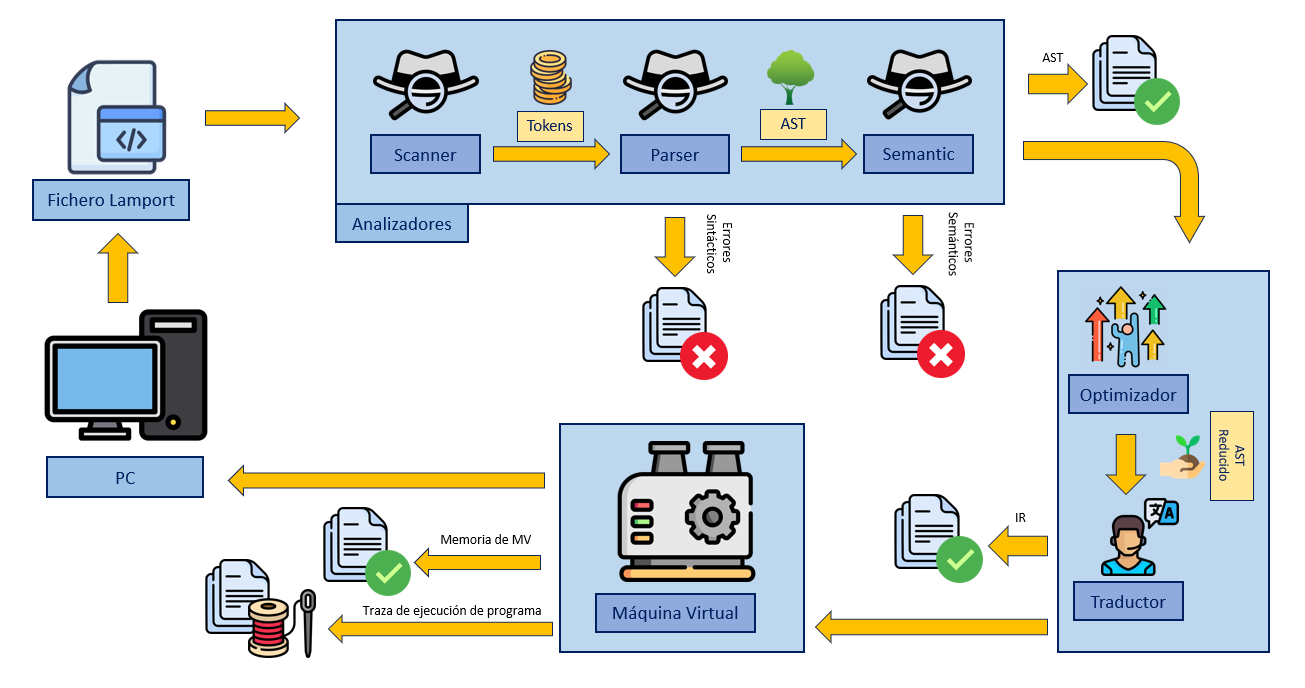
\includegraphics[width=\linewidth]{images/lmp/lmp_resume.png}
    \caption{Esquemático del intérprete de Lamport}
    \label{fig:lmpresume}
\end{figure}



\begin{itemize}
    \item \textbf{Lexer (~\ref{sec:implementacionLexer} ):} Implementa el analizador léxico con Flex. Es el primer módulo encargado de escanear el fichero, reconociendo todos los patrones y obteniendo los tokens.
    
    \item \textbf{Parser (~\ref{sec:implementacionParser} ):} Implementa el analizador sintáctico con Bison. Su función es analizar la secuencia de tokens proporcionada por el Lexer y construir una representación estructurada: un Árbol de Sintaxis Abstracta.
    
    \item \textbf{AST (~\ref{sec:implementacionAST} ):} Representa el Árbol de Sintaxis Abstracta. Es una representación gráfica estructurada del código fuente, que es creada a partir del análisis realizado por el Parser.
    
    \item \textbf{Semantic (~\ref{sec:implementacionSemantic} ):} Encargado del análisis semántico. Evalúa el AST para asegurarse de que el programa cumple con todas las reglas semánticas.
    
    \item \textbf{Error (~\ref{sec:implementacionError} ):} Gestiona y reporta errores encontrados en cualquier etapa de la interpretación, ya sea en el análisis léxico, sintáctico o semántico.
    
    \item \textbf{IR (~\ref{sec:implementacionError} ):} Representa la Representación Intermedia. Es una versión intermedia del código fuente que se utiliza para optimizaciones y para la generación final de código.
    
    \item \textbf{LVM (~\ref{sec:implementacionLVM} ):} Se refiere a la Máquina Virtual de Lamport. Este módulo ejecuta el código representado en IR, actuando como el intérprete final que produce los resultados deseados.
    
    \item \textbf{LMP\_Utils (~\ref{sec:implementacionLMPUtils} ):} Consiste en una serie de controladores que coordinan y facilitan la interacción entre los diferentes módulos del intérprete.
    
\end{itemize}

\section{Módulo de análisis léxico: ``Lexer''}\label{sec:implementacionLexer}
El ``Lexer'' es crucial para la interpretación del lenguaje Lamport, y se ha seleccionado Flex para su implementación por su eficacia y compatibilidad con las especificaciones del lenguaje. Este módulo convierte el código fuente en tokens que luego utiliza el analizador sintáctico para formar el Árbol de Sintaxis Abstracta (AST), actuando como un enlace entre el código y el análisis sintáctico.

\subsection{Diseño y Funcionalidad del Lexer}
El Lexer se desarrolla en un archivo llamado \texttt{lexer.l}, siguiendo la estructura estándar de Flex. Este archivo se divide en secciones clave:

\begin{itemize}
    \item \textbf{Cabeceras y Funciones}: Incluye las bibliotecas necesarias y define funciones auxiliares, facilitando la integración con otras partes del sistema, como el analizador sintáctico.
    \item \textbf{Patrones de Reconocimiento y Acciones Asociadas}: Aquí se establecen las expresiones regulares para identificar tokens del lenguaje Lamport y las acciones correspondientes, como devolver tokens y manejar comentarios y espacios en blanco.
    \item \textbf{Función Central \texttt{yylex()}}: Generada automáticamente por Flex, esta función es el motor del Lexer, encargándose de leer la entrada, identificar patrones y ejecutar acciones asociadas.
\end{itemize}

\subsection{Desafíos y Soluciones en la Implementación}
La interdependencia entre el Lexer y el Parser, especialmente en la definición y reconocimiento de tokens, representa un desafío significativo. Los tokens se definen en una cabecera generada por Bison, requiriendo coordinación entre Flex y Bison. Además, el manejo de cadenas en C plantea desafíos en la memoria dinámica, particularmente al procesar literales e identificadores.

\subsection{Generación del Lexer}
El contenido del fichero \texttt{lexer.l} es procesado por Flex para generar un archivo de código C funcional. Este proceso incluye el manejo detallado de tipos de tokens y cadenas, así como la configuración para el seguimiento preciso de errores por línea. La función \texttt{yylex()} actúa como el núcleo del analizador léxico, proporcionando una interfaz esencial con el analizador sintáctico.

Este enfoque integrado asegura que el Lexer no solo tokenice eficientemente el código fuente de Lamport, sino que también se coordine de manera efectiva con el proceso de análisis sintáctico, contribuyendo así al funcionamiento general del intérprete.
\subsection{Procesamiento de ``Hola Mundo'' utilizando el ``Lexer''}
Ya se dispone de la primera unidad operativa del intérprete, por ello, ya se puede realizar la primera interpretación del programa ``Hola Mundo'' (~\ref{fig:lamportHolaMundo} ). Habilitando un código que permita leer flujos de entrada, y pasando como argumento el fichero donde se encuentra el programa en Lamport, el resultado que muestra el analizador léxico es la siguiente lista:

\begin{figure}[h]
\begin{verbatim}
S_PROGRAM IDENT DELIM_PC
S_VAR IDENT DELIM_2P T_INTEGER DELIM_PC 

S_PROCEDURE IDENT PAR_IZDO IDENT DELIM_2P T_STRING PAR_DCHO 
B_BEGIN 
PRINT PAR_IZDO LITERAL DELIM_C IDENT DELIM_C LITERAL PAR_DCHO DELIM_PC
B_END

S_FUNCTION IDENT PAR_IZDO IDENT DELIM_2P T_INTEGER PAR_DCHO 
    DELIM_2P T_INTEGER DELIM_PC 
S_VAR IDENT DELIM_2P T_INTEGER OP_ASSIGN
    PAR_IZDO OP_MINUS L_INTEGER OP_SUM L_INTEGER PAR_DCHO OP_MULT L_INTEGER 
    OP_MINUS L_INTEGER DELIM_PC
B_BEGIN 
RETURN IDENT OP_SUM IDENT DELIM_PC 
B_END 

S_PROCESS IDENT DELIM_PC 
S_VAR IDENT DELIM_2P T_STRING OP_ASSIGN LITERAL DELIM_PC
S_VAR IDENT DELIM_2P T_INTEGER OP_ASSIGN L_INTEGER DELIM_PC
B_BEGIN 
IDENT PAR_IZDO IDENT PAR_DCHO DELIM_PC 
IDENT OP_ASSIGN IDENT PAR_IZDO IDENT PAR_DCHO DELIM_PC 
PRINT PAR_IZDO LITERAL DELIM_C IDENT PAR_DCHO DELIM_PC 
B_END
\end{verbatim}
\caption{Programa ``¡Hola Mundo!'' Lamport: Secuencia de Tokens.}
\label{fig:tokensHolaMundo}
\end{figure}

\section{Módulo de análisis sintáctico: ``Parser''}\label{sec:implementacionParser}
El analizador sintáctico para el lenguaje Lamport, construido con Bison, juega un papel crucial en la transformación de la secuencia de tokens (proporcionada por el Lexer) en estructuras sintácticas. Bison, conocido por su eficiencia con gramáticas \code{LALR(1)}, ayuda a materializar y procesar la gramática de Lamport.

\subsection{Diseño y Estructura del Parser}
El analizador sintáctico se estructura en el archivo \code{parser.y}, siguiendo las pautas de Bison. Sus componentes principales incluyen:

\begin{itemize}
    \item \textbf{Cabeceras y Funciones}: Incluyen archivos de cabecera y definen funciones utilizadas en el análisis sintáctico.
    \item \textbf{Declaración de Tokens}: Declara tokens provenientes del Lexer.
    \item \textbf{Estructuras para el AST}: Especifica estructuras para construir el Árbol de Sintaxis Abstracta durante el análisis.
    \item \textbf{Asociatividad de Operaciones}: Establece la precedencia de operadores para evitar ambigüedades.
    \item \textbf{Reglas de producción y Acciones semánticas}: Constituyen el núcleo del Parser, definiendo la agrupación de tokens en estructuras sintácticas y permitiendo construir el AST.
\end{itemize}

\subsection{Solucionando los problemas de ambigüedad de la gramática}
Ha llegado el momento de asegurar que los conflictos derivados de la definición ambigüa de la gramática (~\ref{subsubsec:gramaticaAmbiguaLamport} ) se resuelven e implementan de la manera más eficiente para la generación del analizador sintáctico en la práctica.


\noindent
Para generar el analizador sintáctico y además asegurar que no se producen conflictos, se utilizará la siguiente orden:
\begin{verbatim}
    bison --defines=include/lexer/token.h --output=src/parser/parser.c 
        src/parser/parser.y -Wcounterexamples
\end{verbatim}

La opción más notable en este comando es \code{-Wcounterexamples}. Esta opción instruye a Bison a mostrar ejemplos concretos de entrada cuando se detectan conflictos en la gramática. Es especialmente útil ya que no sólo informa de la existencia de un conflicto, sino que también proporciona una entrada específica que lo desencadena, facilitando así la tarea de identificar y corregir el problema en la gramática.

\newpage

\subsubsection{Expresiones}
Si se intenta generar la gramática de Lamport definida en ~\ref{sec:gramaticaLamport} directamente, ocurrirá lo siguiente:
\begin{figure}[h]
    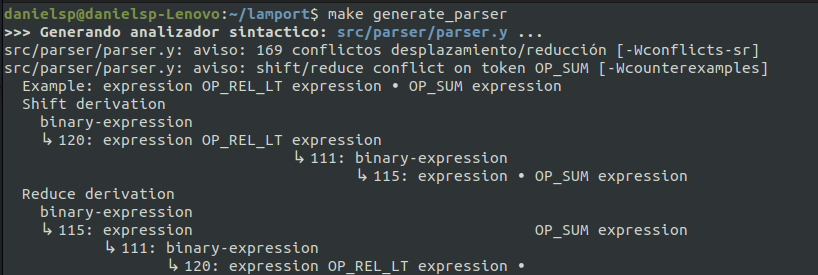
\includegraphics[width=\linewidth]{images/implementacion/parser/parser_conflicts.png}
    \caption{Conflictos de generación de parser por ambigüedad de gramática.}
    \label{fig:parser_conflictos}
\end{figure}

Se producen una inmensa cantidad de conflictos de tipo deslplazamiento/reducción (169 en total). En la captura se observa la indecisión de Bison para decantarse por una regla u otra con el ejemplo siguiente, donde se muestran dos caminos posibles para obtener la misma producción:

\begin{verbatim}
    expression OP_REL_LT expression * OP_SUM expression
\end{verbatim}



La solución para este problema en particular pasa por utilizar la precedencia de los operadores que ya se definió en la sección (~\ref{subsec:precOperadoresLamport} ). En Bison se puede indicar utilizando las directivas:

\begin{verbatim}
    %left <TOKEN>
    %right <TOKEN>
\end{verbatim}

\noindent
donde \code{\%left} y \code{\%right} especifican la asociatividad de las operaciones.



Ahora el resultado es este, donde ya podemos garantizar que $G$ es una gramática \code{LALR(1)}, que es lo que queríamos demostrar al generar la gramática con Bison:
\begin{figure}[h]
    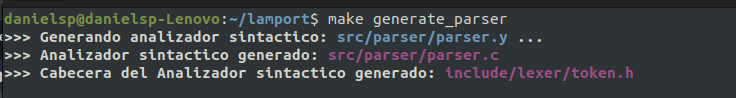
\includegraphics[width=\linewidth]{images/implementacion/parser/parser_success.png}
    \caption{Generación exitosa de la gramática de Lamport.}
    \label{fig:parser_success}
\end{figure}

\subsection{Estrategia de recuperación ante errores sintácticos}
Otro de los problemas a abordar ahora es qué hacer cuando el analizador sintáctico se encuentra con una estructura de tokens que no corresponde con ninguna de las previstas. Aquí hay dos formas posibles de implementar este mecanismo:

\begin{enumerate}
    \item Detectar un error sintáctico y detener inmediatamente el análisis mediante la directiva \code{YYABORT}. Esta acción provoca que, al identificar el primer error en el programa, este sea reconocido y gestionado adecuadamente. Acto seguido, el analizador sintáctico se detendrá, evitando el análisis del resto del fichero.
    
    \item Detectar un error sintáctico e intentar recuperarse, reanudando el análisis a partir de un token específico. En este enfoque, al encontrar un error, se gestiona y, posteriormente, se indica al analizador sintáctico un punto específico dentro de la secuencia de tokens restantes para que continúe con el análisis.
\end{enumerate}

Ambas estrategias son válidas y tienen sus méritos. Sin embargo, es esencial considerar la experiencia del usuario al decidir cuál implementar. La segunda opción, aunque es técnicamente más desafiante debido a la necesidad de identificar los puntos precisos para la recuperación, puede ofrecer una experiencia de usuario más amigable al proporcionar retroalimentación más detallada sobre múltiples errores en lugar de detenerse en el primero. Finalmente, se ha adoptado utilizar un esquema híbrido donde se implementa el primer caso para detección de patrones no esperados y el segundo para detección de errores sintácticos más precisos, como por ejemplo errores en la declaración de una variable.

\section{Árbol de Sintaxis Abstracto (AST)}\label{sec:implementacionAST}
Tras completar el análisis sintáctico, surge la necesidad de representar el programa de una manera que facilite su manipulación y análisis en etapas subsecuentes. En este contexto, se introduce el Árbol de Sintaxis Abstracta (AST, por sus siglas en inglés). Un AST proporciona una representación estructurada y jerárquica de la estructura lógica del código fuente, prescindiendo de muchos detalles superficiales presentes en el texto original. En esta sección, se abordará la construcción y características del AST y se profundizará en su relevancia para el entendimiento y procesamiento del programa Lamport.

\subsection{Nodos del AST}
Dentro de la representación de un Árbol de Sintaxis Abstracta (AST), los nodos desempeñan un papel fundamental. Cada nodo refleja una construcción o elemento del lenguaje de programación, y la estructura jerárquica del árbol establece las relaciones entre estos elementos. En esta subsección, se abordarán los diferentes tipos de nodos que componen el AST, sus características y cómo contribuyen a capturar la esencia semántica del programa Lamport.



En la implementación práctica del AST, los nodos se manejan mediante punteros. Esta elección se justifica por diversas razones. Primero, usar punteros permite una gestión dinámica de memoria, lo que facilita la creación, modificación y eliminación de nodos durante el análisis sintáctico. Además, el uso de punteros posibilita la conexión directa entre nodos para formar la estructura de árbol. Esta metodología también optimiza la eficiencia en términos de memoria y acceso, dado que se evita la duplicación de datos y se permite una referencia directa a la información del nodo.


Todos los nodos citados a continuación han sido definidos mediante un \code{struct}, que es una estructura de datos en C que permite agrupar múltiples variables de diferentes tipos bajo un mismo nombre. Estos \code{structs} proporcionan una manera organizada y coherente de representar información compleja. Así, cada nodo del AST puede contener múltiples campos relevantes para su tipo específico, tales como operadores, operandos, identificadores, entre otros. 


De hecho, la estructura subyacente en la mayoría de los nodos (exceptuando el nodo raíz o padre que representa al programa completo) se basa en el concepto de \textbf{lista enlazada}, una estructura de datos muy utilizada en el ámbito de la programación. Esta estructura se emplea con el objetivo de definir secuencias de nodos de manera eficiente, indicando desde cada nodo la posición del siguiente en la lista.


\noindent
Para cada nodo además se implementaron los siguientes grupos de funciones:

\begin{itemize}
    \item \code{struct node * create_node(...)} : Función encargada de reservar memoria e inicializar un nodo en particular teniendo en cuenta los parámetros que se le han pasado a la función.
    \item \code{void free_node(struct node *)} : Función encargada de liberar la memoria reservada para el nodo pasado como parámetro.
    \item \code{void print_node(struct node *, int depth)} : Función encargada de imprimir el contenido del nodo pasado como parámetro en un flujo de salida. El entero \code{depth} especifica la profundidad del nodo en el árbol, para así poder imprimirlo en el lugar donde corresponde.
\end{itemize}

\noindent
Y en definitiva, estos son los diferentes tipos de nodos considerados:

\begin{enumerate}
    \item \textbf{Nodo de Expresión (expression)}: 
    \begin{itemize}
        \item Almacena información sobre expresiones binarias, unarias, identificadores, literales y llamadas a funciones.
        \item Permite encadenar múltiples expresiones y manejar operaciones complejas.
    \end{itemize}

    \item \textbf{Nodo de Tipo de Dato (type)}:
    \begin{itemize}
        \item Define el tipo de dato (básico, array, especial) de una variable.
        \item Incluye información sobre subtipos y línea de definición.
    \end{itemize}

    \item \textbf{Nodo de Declaración de Variable (declaration)}:
    \begin{itemize}
        \item Contiene identificador, tipo de dato y expresión asignada a una variable.
        \item Permite declarar variables con o sin asignación inicial.
    \end{itemize}

    \item \textbf{Nodo de Sentencia (statement)}:
    \begin{itemize}
        \item Representa diferentes tipos de sentencias (asignación, bucles, if/else, etc.).
        \item Incluye la estructura y la lógica de control y ejecución del programa.
    \end{itemize}

    \item \textbf{Nodo de Parámetro de Subprograma (parameter)}:
    \begin{itemize}
        \item Define los parámetros de subprogramas (funciones y procedimientos).
        \item Incluye nombre, tipo de dato y posición de definición.
    \end{itemize}

    \item \textbf{Nodo de Subprograma (subprogram)}:
    \begin{itemize}
        \item Representa funciones y procedimientos con sus parámetros y cuerpo.
        \item Incluye información de retorno para funciones.
    \end{itemize}

    \item \textbf{Nodo de Proceso (process)}:
    \begin{itemize}
        \item Define procesos, incluyendo nombre, índice y cuerpo de ejecución.
        \item Soporta procesos estáticos vectorizados y maneja declaraciones y sentencias.
    \end{itemize}

    \item \textbf{Nodo de Programa (program)}:
    \begin{itemize}
        \item Nodo raíz del AST que encapsula toda la estructura del programa.
        \item Incluye subprogramas, declaraciones globales y procesos.
    \end{itemize}
\end{enumerate}


\subsection{Integración del AST en el analizador sintáctico}
La integración del AST en el analizador sintáctico generado por Bison se realiza mediante acciones semánticas en las reglas gramaticales. Estas acciones permiten la construcción automática del AST durante el análisis sintáctico. Se emplean directivas específicas (\code{\%union}, \code{\%type}) para definir los tipos de datos que devolverán las reglas gramaticales y asociarlos con las estructuras del AST.

Un enfoque crucial en esta etapa es la gestión de la memoria dinámica, asegurando la reserva y liberación adecuada de memoria para los nodos del AST. Esto incluye estrategias para el manejo eficiente de errores y la prevención de fugas de memoria.

\subsection{Procesamiento de ``Hola Mundo'' utilizando el ``Parser'' con AST}
Ahora ya se puede dar forma a nivel estructural y computacional del código Lamport, y es por ello que ahora que el procesamiento de ``Hola Mundo'' (~\ref{fig:lamportHolaMundo} ) arrojará como resultado el AST que se genere, puesto que el programa es sintácticamente correcto.

\begin{verbatim}
----> PROGRAMA LAMPORT DE NOMBRE: [HolaMundo]
================================================================

----> | DECLARACIONES DE PROGRAMA: [HolaMundo]
|-----> DECLARACION DE VARIABLE: [magico]
|       TIPO DE DATO:
|           TIPO: [integer]
|       VALOR DE INICIALIZACION:
|           <NONE>

================================================================

----> | SUBPROGRAMAS DE PROGRAMA: [HolaMundo]
|-----> NOMBRE DE SUBPROGRAMA: [SaludaUsuario] DE TIPO: [procedure]
|       TIPO DE DATO DE RETORNO:
|   ----> <NONE>
|       PARAMETROS DE SUBPROGRAMA:
|         NOMBRE DE PARAMETRO: [nombre]
|         TIPO DE DATO: [nombre]
|           TIPO: [string]

|       DECLARACIONES DE SUBPROGRAMA:
|-------> <NONE>
|       SENTENCIAS DE SUBPROGRAMA:
|-------> | SENTENCIA DE TIPO: [begin/end block]
|-----------> | SENTENCIA DE TIPO: [print statement]
|             | LISTADO DE EXPRESIONES A IMPRIMIR:
|                > EXPRESION DE TIPO: [literal string]
|                  VALOR DE LITERAL: ["Hola "]
|                > EXPRESION DE TIPO: [identifier]
|                  NOMBRE DE IDENTIFICADOR: [nombre]
|                > EXPRESION DE TIPO: [literal string]
|                  VALOR DE LITERAL: ["!"]



|-----> NOMBRE DE SUBPROGRAMA: [ObtieneNumero] DE TIPO: [function]
|       TIPO DE DATO DE RETORNO:
|         TIPO: [integer]
|       PARAMETROS DE SUBPROGRAMA:
|         NOMBRE DE PARAMETRO: [n]
|         TIPO DE DATO: [n]
|           TIPO: [integer]

|       DECLARACIONES DE SUBPROGRAMA:
|-------> DECLARACION DE VARIABLE: [constant]
|         TIPO DE DATO:
|             TIPO: [integer]
|         VALOR DE INICIALIZACION:
|            > EXPRESION DE TIPO: [binary operation]
|              SIMBOLO DE OPERACION: [-]
|              OPERANDO IZQUIERDO:
|                > EXPRESION DE TIPO: [binary operation]
|                  SIMBOLO DE OPERACION: [*]
|                  OPERANDO IZQUIERDO:
|                    > EXPRESION DE TIPO: [grouped expression]
|                      EXPRESION ENTRE ( )
|                        > EXPRESION DE TIPO: [binary operation]
|                          SIMBOLO DE OPERACION: [+]
|                          OPERANDO IZQUIERDO:
|                            > EXPRESION DE TIPO: [unary operation]
|                              SIMBOLO DE OPERACION: [-]
|                              OPERANDO IZQUIERDO:
|                                > EXPRESION DE TIPO: [literal integer]
|                                  VALOR DE LITERAL: [4]
|                          OPERANDO DERECHO:
|                            > EXPRESION DE TIPO: [literal integer]
|                              VALOR DE LITERAL: [6]
|                  OPERANDO DERECHO:
|                    > EXPRESION DE TIPO: [literal integer]
|                      VALOR DE LITERAL: [10]
|              OPERANDO DERECHO:
|                > EXPRESION DE TIPO: [literal integer]
|                  VALOR DE LITERAL: [2]

|       SENTENCIAS DE SUBPROGRAMA:
|-------> | SENTENCIA DE TIPO: [begin/end block]
|-----------> | SENTENCIA DE TIPO: [return statement]
|             | EXPRESION DE RETORNO:
|                > EXPRESION DE TIPO: [binary operation]
|                  SIMBOLO DE OPERACION: [+]
|                  OPERANDO IZQUIERDO:
|                    > EXPRESION DE TIPO: [identifier]
|                      NOMBRE DE IDENTIFICADOR: [constant]
|                  OPERANDO DERECHO:
|                    > EXPRESION DE TIPO: [identifier]
|                      NOMBRE DE IDENTIFICADOR: [n]



================================================================

----> | PROCESOS DEL PROGRAMA: [HolaMundo]
|-----> | NOMBRE DE PROCESO: [Main] DE TIPO: [individual process]

|-----> | DECLARACIONES DE PROCESO:
|---------> DECLARACION DE VARIABLE: [usuario]
|           TIPO DE DATO:
|               TIPO: [string]
|           VALOR DE INICIALIZACION:
|              > EXPRESION DE TIPO: [literal string]
|                VALOR DE LITERAL: ["Daniel"]

|---------> DECLARACION DE VARIABLE: [numero]
|           TIPO DE DATO:
|               TIPO: [integer]
|           VALOR DE INICIALIZACION:
|              > EXPRESION DE TIPO: [literal integer]
|                VALOR DE LITERAL: [23]


|-----> | SENTENCIAS DE PROCESO:
|---------> | SENTENCIA DE TIPO: [begin/end block]
|-------------> | SENTENCIA DE TIPO: [procedure invocation]
|               | INVOCACION DE PROCEDIMIENTO DE NOMBRE: [SaludaUsuario]
|               | LISTADO DE ARGUMENTOS DE INVOCACION DEL PROCEDIMIENTO:
|                  > EXPRESION DE TIPO: [identifier]
|                    NOMBRE DE IDENTIFICADOR: [usuario]

|-------------> | SENTENCIA DE TIPO: [assignment]
|               | ASIGNACION A VARIABLE: [magico]
|               | EXPRESION ASIGNADA A VARIABLE:
|                  > EXPRESION DE TIPO: [function invocation]
|                    INVOCACION DE FUNCION DE NOMBRE: [ObtieneNumero]
|                    LISTADO DE ARGUMENTOS DE INVOCACION DE FUNCION:
|                      > EXPRESION DE TIPO: [identifier]
|                        NOMBRE DE IDENTIFICADOR: [numero]

|-------------> | SENTENCIA DE TIPO: [print statement]
|               | LISTADO DE EXPRESIONES A IMPRIMIR:
|                  > EXPRESION DE TIPO: [literal string]
|                    VALOR DE LITERAL: ["El numero magico vale: "]
|                  > EXPRESION DE TIPO: [identifier]
|                    NOMBRE DE IDENTIFICADOR: [magico]
\end{verbatim}
\begin{figure}[hbtp]
\caption{Programa ``¡Hola Mundo!'' Lamport: Resultado de análisis sintáctico (AST).}
\label{fig:ASTHolaMundo}
\end{figure}

\section{Módulo de análisis semántico: ``Semantic''}\label{sec:implementacionSemantic}
El análisis semántico en el lenguaje Lamport verifica la coherencia y correctitud del código más allá de la gramática, enfocándose en las reglas de contexto y las relaciones semánticas. Este módulo es importante para asegurar que el código tenga un significado lógico y esté listo para la interpretación.

\subsection{La tabla de Símbolos}
La tabla de símbolos es un registro organizado de todas las entidades definidas en el código, como variables, constantes, funciones y procedimientos. Esta tabla almacena información crucial, incluyendo tipo, alcance y, en algunos casos, valores iniciales o información de memoria.

\subsubsection{Ámbito de variable (scope) y Tabla de Símbolos}
El ámbito de una variable, o su \textit{scope}, define su accesibilidad en el código, pudiendo ser global (accesible en todo el programa) o local (limitada a un bloque específico). Para manejar los ámbitos eficientemente, se utiliza una tabla hash en la tabla de símbolos. Esta estructura, que asocia claves (nombres de símbolos) con valores (información del símbolo), permite un acceso rápido y eficiente a los datos mediante funciones hash.

\subsubsection{Implementación de la tabla con una pila de tablas hash}
La gestión de los diferentes ámbitos se realiza a través de una pila de tablas hash. Al entrar en un nuevo ámbito, como un subprograma o proceso, se añade una tabla hash vacía a la cima de la pila, donde los símbolos definidos en ese ámbito se almacenarán. Al salir del ámbito, la tabla hash correspondiente se retira, eliminando los símbolos de ese ámbito específico. Esta estructura facilita la resolución de referencias a símbolos, siempre resolviendo al símbolo más cercano en términos de ámbito.

Para llevar a cabo esta tarea, se deben enfrentar varios desafíos. En primer lugar, es necesario identificar y gestionar los distintos ámbitos o ``scopes'' en los que un nombre puede estar definido. Como se ha visto en secciones anteriores, la estructura de una pila de tablas hash es útil en este aspecto. Cada ámbito tiene su propia tabla hash, y al buscar un nombre, se consulta primero la tabla del ámbito actual, avanzando hacia ámbitos más externos si es necesario.

\subsection{Resolución de nombres}
El análisis semántico comienza con la resolución de nombres, determinando a qué entidad del programa se refiere un nombre en un contexto dado. Esta fase es crucial para garantizar la coherencia y correcta ejecución del código, empleando la estructura de la pila de tablas hash para identificar correctamente los ámbitos y resolver las referencias a símbolos

El esquema general del algoritmo de resolución de nombres es el siguiente, aplicándolo desde el nodo raíz del AST (\code{program}):
\begin{enumerate}
    \item Al inicio del análisis:
    \begin{enumerate}
        \item Insertar el ``scope'' global en la pila.
    \end{enumerate}
    \item Si se trata de un bloque de declaraciones:
    \begin{enumerate}
        \item Comprobar si ya existe un símbolo en la tabla de símbolos para la variable actual a analizar.
        \begin{itemize}
            \item En caso afirmativo, se trata de un \textbf{error de redefinición de variable}.
            \item En otro caso, se crea el símbolo y se inserta en el ``scope''.
        \end{itemize}
        \item Continuar con el resto de variables hasta que no queden.
    \end{enumerate}
    \item Si se trata de un bloque de sentencias/expresiones:
    \begin{itemize}
        \item Aplicar resolución de nombres a cada sentencia o expresión hasta que no queden, buscando en todos los scopes las posibles referencias a símbolos que puedan haber.
        \begin{itemize}
            \item Si no se encuentra una referencia a un símbolo dentro de unas estructuras, se trata de un \textbf{error de uso de símbolo no declarado}, ya sea de variable, subprograma o proceso.
        \end{itemize}
    \end{itemize}
    \item Si se trata de un bloque de subprogramas:
    \begin{enumerate}
        \item Comprobar para el scope global y para el subprograma actual a analizar si ya existe un símbolo en la tabla de símbolos asociado a su identificador.
        \begin{itemize}
            \item En caso afirmativo, se tata de un \textbf{error de redefinición de subprograma}.
            \item En otro caso, se crea el símbolo y se inserta en el ``scope''.
        \end{itemize}
        \item Insertar un nuevo ``scope'' en la pila.
        \item Aplicar resolución de nombres a las declaraciones del subprograma.
        \item Aplicar resolución de nombres a las sentencias del subprograma.
        \item Retirar el ``scope'' actual de la pila.

        \item Continuar con el resto de subprogramas hasta que no queden.
    \end{enumerate}
    \item Si se trata de un bloque de procesos:
    \begin{enumerate}
        \item Comprobar para el scope global y para el proceso actual a analizar si ya existe un símbolo en la tabla de símbolos asociado a su identificador.
        \begin{itemize}
            \item En caso afirmativo, se tata de un \textbf{error de redefinición de proceso}.
            \item En otro caso, se crea el símbolo y se inserta en el ``scope''.
        \end{itemize}
        \item Insertar un nuevo ``scope'' en la pila.
        \item Aplicar resolución de nombres a las declaraciones del proceso.
        \item Aplicar resolución de nombres a las sentencias del proceso.
        \item Retirar el ``scope'' actual de la pila.

        \item Continuar con el resto de procesos hasta que no queden.
    \end{enumerate}
\end{enumerate}

\subsection{Comprobación de tipos}
Esta fase garantiza que las operaciones y asignaciones realizadas en el código fuente son coherentes desde el punto de vista de los tipos de datos involucrados. Así, se evita que, por ejemplo, se intente sumar un número entero con una cadena de texto o que se asigne un valor de tipo real a una variable que espera un valor booleano.



La comprobación de tipos no solo proporciona seguridad en la ejecución al detectar errores potenciales en una etapa temprana del proceso de compilación, sino que también contribuye a la claridad y robustez del código. Aquí es donde entra en juego la descripción semántica que se hizo del lenguaje Lamport en ~\ref{subsec:semanticaLamport}, porque se aplicará directamente en este apartado del analizador semántico.



Con respecto a la comprobación de tipos \textit{per se} no hay ninguna dificultad técnica. La forma de proceder es prácticamente idéntica a la del algoritmo de resolución de nombres, recorriendo el AST comprobando todos los nodos importantes:

\begin{enumerate}
    \item Si se trata de una expresión:
    \begin{itemize}
        \item Comprobar que se verifican todas las restricciones semánticas definidas en ~\ref{subsubsec:restriccionesSemanticas} y que refieren a expresiones.
        \item En caso contrario, se produce un \textbf{error de comprobación de tipos entre operandos de expresión}.
        \item En el caso de una expresión de llamada a función, se debe comprobar que el tipo de los argumentos pasados coincide con el de los parámetros que se definieron para la función, en el mismo orden en el que aparecen éstos.
    \end{itemize}
    \item Si se trata de una declaración de variable y además tiene un valor de inicio:
    \begin{itemize}
        \item Comprobar que el tipo de dato de la variable coincide con la evaluación del tipo de dato que emite la expresión de inicialización.
        \item En caso contrario, se produce un \textbf{error de asignación de tipos}.
    \end{itemize}
    \item Si se trata de un subprograma:
    \begin{itemize}
        \item Comprobar que se verifican todas las restricciones semánticas definidas en ~\ref{subsubsec:restriccionesSemanticas} y que refieren a subprogramas.
        \item En caso contrario, se produce un \textbf{error de comprobación de tipos}.
    \end{itemize}
    \item Si se trata de una sentencia:
    \begin{itemize}
        \item Si se está realizando una sentencia de asignación, mismo tratamiento que en el caso de inicialización de variables.
        \item En el caso de bucles while y estructuras if/else, la expresión de condición debe emitir el tipo \code{boolean}.
        \item En el caso de bucles for, las expresiones de inicio y fin deben emitir el tipo \code{integer}.
        \item En el caso de una llamada a procedimiento, se debe comprobar que el tipo de los argumentos pasados coincide con el de los parámetros que se definieron para el procedimiento, en el mismo orden en el que aparecen éstos.
        \item Todo lo anterior que no se verifique será un \textbf{error de comprobación de tipos ó de asignación}.
    \end{itemize}
\end{enumerate}

\subsection{Procesamiento de ``Hola Mundo'' utilizando el ``Semantic''}
Ahora ya se dispone de todos los analizadores posibles para un lenguaje de programación cualquiera, en particular para el lenguaje Lamport. Adaptando el código del intérprete ahora cuando se supere la fase del analizador sintáctico, se recorrerá el AST generado analizando semánticamente el programa. Primero se aplica resolución de nombres y posteriormente la comprobación de tipos. Si el procesamiento de ``Hola Mundo'' (~\ref{fig:lamportHolaMundo} ) se ha superado, se verá un mensaje de éxito en pantalla. En caso contrario se mostrarán todos los errores semánticos emitidos:



\noindent
Puesto que el programa es semánticamente correcto, el mensaje que se muestra es:
\begin{verbatim}
    ``RESOLUCIÓN DE NOMBRES Y COMPROBACIÓN DE TIPOS 
        REALIZADOS CON ÉXITO.''
\end{verbatim}

\section{Módulo de gestión de errores: ``Error''}\label{sec:implementacionError}
Para manejar errores en los análisis sintáctico y semántico, se ha desarrollado un módulo específico de gestión de errores. Se utiliza una estructura común \code{error} que registra el tipo de error (sintáctico o semántico), la línea del error, un mensaje descriptivo y un puntero al siguiente error. La estructura también incluye detalles adicionales sobre errores específicos, tanto sintácticos como semánticos.

Este módulo de errores se integra tanto en el análisis sintáctico como en el semántico, marcando errores en las reglas sintácticas y a lo largo de los algoritmos semánticos. El orden de aparición de los errores depende de la fase de análisis:

\begin{enumerate}
    \item Si no se supera el análisis sintáctico, se imprimen los errores sintácticos.
    \item Si se supera el análisis sintáctico pero no la resolución de nombres, se imprimen los errores semánticos relacionados.
    \item Si no se supera la comprobación de tipos, se imprimen los errores semánticos correspondientes.
\end{enumerate}


\section{Módulo de gestión de Representación Intermedia: ``IR''}\label{sec:implementacionIR}
La Representación Intermedia (IR) es una fase fundamental en la transformación y optimización del código fuente de Lamport. Este módulo actúa como un puente entre el análisis semántico y la traducción final o interpretación del código, optimizando las operaciones posteriores mediante una estructura común y coherente.

\subsection{Elección de Representación Intermedia}
La IR elegida para este proyecto se basa en registros, con un conjunto de instrucciones que detallan el manejo de estos registros. Esta estructura facilita la simulación del funcionamiento de un sistema concurrente y simplifica la representación del código.

\noindent
Una instrucción consta de los siguientes elementos:

\begin{itemize}
    \item \textbf{Código de instrucción}: Es un identificador que sirve para indicar a la posterior máquina virtual el tipo de instrucción que va a ejecutar.
    \item \textbf{Operando de destino}: Identificador que representa el lugar donde el resultado de la acción que realizará la entidad que ejecute la instrucción se almacenará.
    \item \textbf{Operando 1}: Identificador que representa al dato del primer operando de la instrucción.
    \item \textbf{Operando 2}: Identificador que representa al dato del segundo operando de la instrucción.
\end{itemize}

Los operandos son elementos que determinan las fuentes de datos o valores con los que se realizará la operación indicada por el código de instrucción. Estos pueden ser constantes, registros, direcciones de memoria, entre otros. La cantidad y el tipo de operandos pueden variar según la instrucción, y su correcta interpretación es crucial para el adecuado funcionamiento de la máquina virtual y la ejecución del programa. En esta representación intermedia, hay estos tipos de operandos:

\begin{itemize}
    \item \textbf{Identificación de un registro}: El operando apunta a un registro de la máquina virtual.
    \item \textbf{Identificación de un literal}: El operando apunta a un literal.
    \item \textbf{Identificación de una variable}: El operando apunta a una variable.
    \item \textbf{Identificación de una variable array}: El operando apunta a un elemento en concreto de una variable array.
    \item \textbf{Identificación de una etiqueta}: El operando apunta a la dirección de una etiqueta.
    \item \textbf{Identificación de un proceso/hebra}: El operando contiene el identificador del proceso.
    \item \textbf{Identificación de un salto directo}: El operando contiene la dirección de la siguiente instrucción a la que el proceso debe saltar. Tiene un comportamiento similar al de una etiqueta, pero sin especificar un nombre para la misma.
\end{itemize}

Finalmente, en este lenguaje de representación intermedia hay un total de \textbf{5 tipos de instrucciones diferentes}:

\begin{itemize}
    \item \textbf{1 destino y 2 operandos}: la instrucción a ejecutar necesita de dos operandos y el resultado se almacenará en un destino.
    \item \textbf{1 destino y 1 operando}: la instrucción a ejecutar necesita un operando y el resultado se almacena en un destino.
    \item \textbf{1 operando}: la instrucción a ejecutar necesita un operando, y no hay necesidad de almacenar el resultado de la acción.
    \item \textbf{0 destinos y 2 operandos}: la instrucción dispone de dos operandos pero no se almacena el resultado de la ejecución en un destino.
    \item \textbf{0 destinos y 0 operandos}: la instrucción sólo dispone de su código de instrucción, suficiente para su ejecución.
\end{itemize}

\subsection{Repertorio de instrucciones de IR}
A continuación se realiza un estudio detallado del repertorio de instrucciones definido para la representación intermedia del lenguaje Lamport.

\renewcommand{\arraystretch}{1.5}
\begin{longtable}{|c|c|c|c|c|}
\caption{Repertorio de instrucciones de Representación Intermedia.} \label{tab:instruccionesIR} \\
\hline
\textbf{CÓDIGO} & \textbf{DETALLES} & \textbf{OP. DEST.} & \textbf{OP. 1} & \textbf{OP. 2} \\
\hline
\endfirsthead

\multicolumn{5}{c}%
{{\bfseries \tablename\ \thetable{} -- continuación de la página anterior}} \\
\hline
\textbf{CÓDIGO} & \textbf{DETALLES} & \textbf{OP. DEST.} & \textbf{OP. 1} & \textbf{OP. 2} \\
\hline
\endhead

\hline \multicolumn{5}{|r|}{{Continúa en la siguiente página}} \\
\hline
\endfoot

\hline
\endlastfoot
\code{IR_LABEL} & ~\ref{subsubsec:IR_LABEL}  & NO & SÍ & NO \\
\hline
\code{IR_OP_LOAD} & ~\ref{subsubsec:IR_OP_LOAD}  & SÍ & SÍ & NO \\
\hline
\code{IR_OP_STORE} & ~\ref{subsubsec:IR_OP_STORE} & SÍ & SÍ & NO \\
\hline
\code{IR_OP_ADD_[I|F]} \footnote{Aquí y en el resto de instrucciones aritméticas, ``I'' denota que la instrucción involucra a operandos de tipo \textbf{entero}, mientras que ``F'' hace lo mismo con operandos de tipo \textbf{real}.} & ~\ref{subsubsec:IR_OP_ADD} & SÍ & SÍ & SÍ \\
\hline
\code{IR_OP_SUB_[I|F]} & ~\ref{subsubsec:IR_OP_SUB} & SÍ & SÍ & SÍ \\
\hline
\code{IR_OP_MULT_[I|F]} & ~\ref{subsubsec:IR_OP_MULT} & SÍ & SÍ & SÍ \\
\hline
\code{IR_OP_DIV_[I|F]} & ~\ref{subsubsec:IR_OP_DIV} & SÍ & SÍ & SÍ \\
\hline
\code{IR_OP_MOD_I} & ~\ref{subsubsec:IR_OP_MOD} & SÍ & SÍ & SÍ \\
\hline
\code{IR_OP_NEG_[I|F]} & ~\ref{subsubsec:IR_OP_NEG} & SÍ & SÍ & SÍ \\
\hline
\code{IR_OP_AND} & ~\ref{subsubsec:IR_OP_AND} & SÍ & SÍ & SÍ \\
\hline
\code{IR_OP_OR} & ~\ref{subsubsec:IR_OP_OR} & SÍ & SÍ & SÍ \\
\hline
\code{IR_OP_NOT} & ~\ref{subsubsec:IR_OP_NOT} & SÍ & SÍ & SÍ \\
\hline
\code{IR_OP_CMP_LT} & ~\ref{subsubsec:IR_OP_CMP_LT} & SÍ & SÍ & SÍ \\
\hline
\code{IR_OP_CMP_LTE} & ~\ref{subsubsec:IR_OP_CMP_LTE} & SÍ & SÍ & SÍ \\
\hline
\code{IR_OP_CMP_GT} & ~\ref{subsubsec:IR_OP_CMP_GT} & SÍ & SÍ & SÍ \\
\hline
\code{IR_OP_CMP_GTE} & ~\ref{subsubsec:IR_OP_CMP_GTE} & SÍ & SÍ & SÍ \\
\hline
\code{IR_OP_CMP_EQ} & ~\ref{subsubsec:IR_OP_CMP_EQ} & SÍ & SÍ & SÍ \\
\hline
\code{IR_OP_CMP_NEQ} & ~\ref{subsubsec:IR_OP_CMP_NEQ} & SÍ & SÍ & SÍ \\
\hline
\code{IR_OP_JMP} & ~\ref{subsubsec:IR_OP_JMP} & NO & SÍ & NO \\
\hline
\code{IR_OP_JMP_TRUE} & ~\ref{subsubsec:IR_OP_JMP_TRUE} & NO & SÍ & NO \\
\hline
\code{IR_OP_JMP_FALSE} & ~\ref{subsubsec:IR_OP_JMP_FALSE} & NO & SÍ & NO \\
\hline
\code{IR_OP_CALL} & ~\ref{subsubsec:IR_OP_CALL} & NO & SÍ & NO \\
\hline
\code{IR_OP_RET} & ~\ref{subsubsec:IR_OP_RET} & NO & SÍ & NO \\
\hline
\code{IR_OP_PUSH} & ~\ref{subsubsec:IR_OP_PUSH} & NO & SÍ & NO \\
\hline
\code{IR_OP_POP} & ~\ref{subsubsec:IR_OP_POP} & NO & SÍ & NO \\
\hline
\code{IR_OP_PRINT} & ~\ref{subsubsec:IR_OP_PRINT} & NO & SÍ & NO \\
\hline
\code{IR_END_PRINT} & ~\ref{subsubsec:IR_END_PRINT} & NO & NO & NO \\
\hline
\code{IR_START_PROGRAM} & ~\ref{subsubsec:IR_START_PROGRAM} & NO & NO & NO \\
\hline
\code{IR_END_PROGRAM} & ~\ref{subsubsec:IR_END_PROGRAM} & NO & NO & NO \\
\hline
\code{IR_START_PROCESS} & ~\ref{subsubsec:IR_START_PROCESS} & NO & SÍ & NO \\
\hline
\code{IR_START_DPROCESS} & ~\ref{subsubsec:IR_START_DPROCESS} & SÍ & SÍ & SÍ \\
\hline
\code{IR_END_PROCESS} & ~\ref{subsubsec:IR_END_PROCESS} & NO & SÍ & NO \\
\hline
\code{IR_WAIT_PROCESS} & ~\ref{subsubsec:IR_WAIT_PROCESS} & NO & SÍ & NO \\
\hline
\code{IR_SLEEP_PROCESS} & ~\ref{subsubsec:IR_SLEEP_PROCESS} & NO & SÍ & NO \\
\hline
\code{IR_OP_ATOMIC_BEGIN} & ~\ref{subsubsec:IR_OP_ATOMIC_BEGIN} & NO & NO & NO \\
\hline
\code{IR_OP_ATOMIC_END} & ~\ref{subsubsec:IR_OP_ATOMIC_END} & NO & NO & NO \\
\hline
\code{IR_OP_SEM_WAIT} & ~\ref{subsubsec:IR_OP_SEM_WAIT} & NO & SÍ & NO \\
\hline
\code{IR_OP_SEM_SIGNAL} & ~\ref{subsubsec:IR_OP_SEM_SIGNAL} & NO & SÍ & NO \\
\hline
\code{IR_START_INIT_GLOBAL_VAR} & ~\ref{subsubsec:IR_START_INIT_GLOBAL_VAR} & NO & NO & NO \\
\hline
\code{IR_END_GLOBAL_VAR} & ~\ref{subsubsec:IR_END_INIT_GLOBAL_VAR} & NO & NO & NO \\
\end{longtable}
\renewcommand{\arraystretch}{1.0}

\subsubsection{Instrucción IR\_LABEL}\label{subsubsec:IR_LABEL}
\noindent
\textbf{Funcionalidad:} Representa a una etiqueta

\noindent
\textbf{Argumentos:} La estructura de la instrucción es la siguiente:
\begin{verbatim}
IR_LABEL <operando1>
\end{verbatim}
\begin{itemize}
    \item <\code{operando1}>: Etiqueta que delimita una sección.
\end{itemize}

\noindent
\textbf{Ejecución de la instrucción:}


\noindent
Se incrementa el contador de programa y se sigue el flujo de ejecución normal.


\noindent
\textbf{Ejemplo de uso:}
\begin{verbatim}
IR_LABEL etq1
\end{verbatim}

\subsubsection{Instrucción IR\_OP\_LOAD}\label{subsubsec:IR_OP_LOAD}
\noindent
\textbf{Funcionalidad:} Carga un valor de una variable en un registro.

\noindent
\textbf{Argumentos:} La estructura de la instrucción es la siguiente:
\begin{verbatim}
IR_OP_LOAD <registro_destino> <operando1>
\end{verbatim}
\begin{itemize}
    \item <\code{registro_destino}>: registro donde se almacenará el valor de la variable.
    \item <\code{operando1}>: Es una \code{variable}. Su valor se cargará en el registro de destino.
\end{itemize}

\noindent
\textbf{Ejecución de la instrucción:}
\noindent
Se realizan los siguientes pasos para la ejecución de la instrucción:

\begin{enumerate}
    \item El valor de <\code{operando1}> se carga en <\code{registro_destino}>.
\end{enumerate}

\noindent
\textbf{Ejemplo de uso:}
\noindent
Suponiendo que \code{y} es una variable:

\begin{verbatim}
IR_OP_LOAD R1, y
\end{verbatim}

\noindent
\textbf{Comentarios adicionales:}

La representación a nivel de código de esta instrucción realmente contendrá en el operando un entero apuntador a una tabla de variables indexada donde se encuentra el nombre de dicha variable \texttt{y}.

\subsubsection{Instrucción IR\_OP\_STORE}\label{subsubsec:IR_OP_STORE}
\noindent
\textbf{Funcionalidad:} Almacena el valor de un registro en una variable.

\noindent
\textbf{Argumentos:} La estructura de la instrucción es la siguiente:

\begin{verbatim}
IR_OP_STORE <registro_fuente> <operando1>
\end{verbatim}
\begin{itemize}
    \item <\code{registro_fuente}>: registro del cual se tomará el valor para almacenarlo en la variable.
    \item <\code{operando1}>: Es una \code{variable}. Se almacenará el valor del registro fuente en esta variable.
\end{itemize}

\noindent
\textbf{Ejecución de la instrucción:}
\noindent
Se realizan los siguientes pasos para la ejecución de la instrucción:

\begin{enumerate}
    \item El valor de <\code{registro_fuente}> se almacena en <\code{operando1}>.
\end{enumerate}

\noindent
\textbf{Ejemplo de uso:}
\noindent
Suponiendo que \code{z} es una variable:

\begin{verbatim}
IR_OP_STORE R2, z
\end{verbatim}

\noindent
\textbf{Comentarios adicionales:}

La representación a nivel de código de esta instrucción realmente contendrá en el operando un entero apuntador a una tabla de variables indexada donde se encuentra el nombre de dicha variable \texttt{z}.

\subsubsection{Instrucción IR\_OP\_ADD\_[I|F]}\label{subsubsec:IR_OP_ADD}
\noindent
\textbf{Funcionalidad:} Suma dos operandos y almacena el resultado en un registro.

\noindent
\textbf{Argumentos:} La estructura de la instrucción es la siguiente:
\begin{verbatim}
IR_OP_ADD_[I|F] <registro_destino> <operando1> <operando2>
\end{verbatim}
\begin{itemize}
    \item <\code{registro_destino}>: registro donde se almacenará el resultado de la suma.
    \item <\code{operando1}, \code{operando2}>: Operandos a sumar.
\end{itemize}

\noindent
\textbf{Ejecución de la instrucción:}


\noindent
El valor de <\code{operando1}> se suma al valor de <\code{operando2}>, y el resultado se almacena en <\code{registro_destino}>.


\noindent
\textbf{Ejemplo de uso:}
\begin{verbatim}
IR_OP_ADD_I R1, R2, R3
IR_OP_ADD_F R2, R3, R4
\end{verbatim}

\subsubsection{Instrucción IR\_OP\_SUB\_[I|F]}\label{subsubsec:IR_OP_SUB}
\noindent
\textbf{Funcionalidad:} Resta el segundo operando al primero y almacena el resultado en un registro.

\noindent
\textbf{Argumentos:} La estructura de la instrucción es la siguiente:
\begin{verbatim}
IR_OP_SUB_[I|F] <registro_destino> <operando1> <operando2>
\end{verbatim}
\begin{itemize}
    \item <\code{registro_destino}>: registro donde se almacenará el resultado de la resta.
    \item <\code{operando1}, \code{operando2}>: Operandos involucrados en la resta.
\end{itemize}

\noindent
\textbf{Ejecución de la instrucción:}
\vspace{0.3cm}

\noindent
El valor de <\code{operando2}> se resta del valor de <\code{operando1}>, y el resultado se almacena en <\code{registro_destino}>.
\vspace{0.3cm}

\noindent
\textbf{Ejemplo de uso:}
\begin{verbatim}
IR_OP_SUB_F R1, R2, R3
\end{verbatim}

\subsubsection{Instrucción IR\_OP\_MULT\_[I|F]}\label{subsubsec:IR_OP_MULT}
\noindent
\textbf{Funcionalidad:} Multiplica dos operandos y almacena el resultado en un registro.

\noindent
\textbf{Argumentos:} La estructura de la instrucción es la siguiente:
\begin{verbatim}
IR_OP_MULT_[I|F] <registro_destino> <operando1> <operando2>
\end{verbatim}
\begin{itemize}
    \item <\code{registro_destino}>: registro donde se almacenará el resultado de la multiplicación.
    \item <\code{operando1}, \code{operando2}>: Operandos a multiplicar.
\end{itemize}

\noindent
\textbf{Ejecución de la instrucción:}
\vspace{0.3cm}

\noindent
El valor de <\code{operando1}> se multiplica por el valor de <\code{operando2}>, y el resultado se almacena en <\code{registro_destino}>.
\vspace{0.3cm}

\noindent
\textbf{Ejemplo de uso:}
\begin{verbatim}
IR_OP_MULT_I R1, R2, R3
\end{verbatim}

\subsubsection{Instrucción IR\_OP\_DIV\_[I|F]}\label{subsubsec:IR_OP_DIV}
\noindent
\textbf{Funcionalidad:} Divide el primer operando entre el segundo y almacena el resultado en un registro.

\noindent
\textbf{Argumentos:} La estructura de la instrucción es la siguiente:
\begin{verbatim}
IR_OP_DIV_[I|F] <registro_destino> <operando1> <operando2>
\end{verbatim}
\begin{itemize}
    \item <\code{registro_destino}>: registro donde se almacenará el resultado de la división.
    \item <\code{operando1}, \code{operando2}>: Operandos involucrados en la división.
\end{itemize}

\noindent
\textbf{Ejecución de la instrucción:}
\vspace{0.3cm}

\noindent
El valor de <\code{operando1}> se divide entre el valor de <\code{operando2}>, y el resultado se almacena en <\code{registro_destino}>.
\vspace{0.3cm}

\noindent
\textbf{Ejemplo de uso:}
\begin{verbatim}
IR_OP_DIV_F R1, R2, R3
\end{verbatim}

\subsubsection{Instrucción IR\_OP\_MOD\_I}\label{subsubsec:IR_OP_MOD}
\noindent
\textbf{Funcionalidad:} Calcula el residuo de la división del primer operando entre el segundo y almacena el resultado en un registro.

\noindent
\textbf{Argumentos:} La estructura de la instrucción es la siguiente:
\begin{verbatim}
IR_OP_MOD_I <registro_destino> <operando1> <operando2>
\end{verbatim}
\begin{itemize}
    \item <\code{registro_destino}>: registro donde se almacenará el resultado del cálculo del residuo.
    \item <\code{operando1}, \code{operando2}>: Operandos involucrados en el cálculo del residuo.
\end{itemize}

\noindent
\textbf{Ejecución de la instrucción:}
\vspace{0.3cm}

\noindent
El residuo de la división del valor de <\code{operando1}> entre el valor de <\code{operando2}> se calcula, y el resultado se almacena en <\code{registro_destino}>.
\vspace{0.3cm}

\noindent
\textbf{Ejemplo de uso:}
\begin{verbatim}
IR_OP_MOD_I R1, R2, R3
\end{verbatim}

\subsubsection{Instrucción IR\_OP\_NEG\_[I|F]}\label{subsubsec:IR_OP_NEG}
\noindent
\textbf{Funcionalidad:} Realiza la negación aritmética del operando y almacena el resultado en un registro.

\noindent
\textbf{Argumentos:} La estructura de la instrucción es la siguiente:
\begin{verbatim}
IR_OP_NEG_[I|F] <registro_destino> <operando1>
\end{verbatim}
\begin{itemize}
    \item <\code{registro_destino}>: registro donde se almacenará el resultado de la negación.
    \item <\code{operando1}>: operando a negar.
\end{itemize}

\noindent
\textbf{Ejecución de la instrucción:}
\vspace{0.3cm}

\noindent
Se niega el valor de <\code{operando1}> y el resultado se almacena en \\
<\code{registro_destino}>.
\vspace{0.3cm}

\noindent
\textbf{Ejemplo de uso:}
\begin{verbatim}
IR_OP_NEG_I R0, R1
\end{verbatim}

\subsubsection{Instrucción IR\_OP\_AND}\label{subsubsec:IR_OP_AND}
\noindent
\textbf{Funcionalidad:} Realiza la conjunción lógica entre dos operandos y almacena el resultado en un registro.

\noindent
\textbf{Argumentos:} La estructura de la instrucción es la siguiente:
\begin{verbatim}
IR_OP_AND <registro_destino> <operando1> <operando2>
\end{verbatim}
\begin{itemize}
    \item <\code{registro_destino}>: registro donde se almacenará el resultado de la conjunción lógica.
    \item <\code{operando1}, \code{operando2}>: operandos de la conjunción lógica.
\end{itemize}

\noindent
\textbf{Ejecución de la instrucción:}
\vspace{0.3cm}

\noindent
Se realiza AND lógico entre los valores de <\code{operando1}> y <\code{operando2}> y el resultado se almacena en <\code{registro_destino}>.
\vspace{0.3cm}

\noindent
\textbf{Ejemplo de uso:}
\begin{verbatim}
IR_OP_AND R0, R1, $true
\end{verbatim}

\subsubsection{Instrucción IR\_OP\_OR}\label{subsubsec:IR_OP_OR}
\noindent
\textbf{Funcionalidad:} Realiza la disyunción lógica entre dos operandos y almacena el resultado en un registro.

\noindent
\textbf{Argumentos:} La estructura de la instrucción es la siguiente:
\begin{verbatim}
IR_OP_OR <registro_destino> <operando1> <operando2>
\end{verbatim}
\begin{itemize}
    \item <\code{registro_destino}>: registro donde se almacenará el resultado de la disyunción lógica.
    \item <\code{operando1}, \code{operando2}>: operandos de la disyunción lógica.
\end{itemize}

\noindent
\textbf{Ejecución de la instrucción:}
\vspace{0.3cm}

\noindent
Se realiza OR lógico entre los valores de <\code{operando1}> y <\code{operando2}> y el resultado se almacena en <\code{registro_destino}>.
\vspace{0.3cm}

\noindent
\textbf{Ejemplo de uso:}
\begin{verbatim}
IR_OP_OR R0, R1, R2
\end{verbatim}

\subsubsection{Instrucción IR\_OP\_NOT}\label{subsubsec:IR_OP_NOT}
\noindent
\textbf{Funcionalidad:} Realiza la negación lógica de un operando y almacena el resultado en un registro.

\noindent
\textbf{Argumentos:} La estructura de la instrucción es la siguiente:
\begin{verbatim}
IR_OP_NOT <registro_destino> <operando1>
\end{verbatim}
\begin{itemize}
    \item <\code{registro_destino}>: registro donde se almacenará el resultado de la operación lógica.
    \item <\code{operando1}>: operando de negación lógica. Puede ser: registro, literal.
\end{itemize}

\noindent
\textbf{Ejecución de la instrucción:}
\vspace{0.3cm}

\noindent
Se realiza NOT lógico de <\code{operando1}> y el resultado se almacena en <\code{registro_destino}>.
\vspace{0.3cm}

\noindent
\textbf{Ejemplo de uso:}
\begin{verbatim}
IR_OP_NOT R0, R1
\end{verbatim}


\subsubsection{Instrucción IR\_OP\_CMP\_LT}\label{subsubsec:IR_OP_CMP_LT}
\noindent
\textbf{Funcionalidad:} Compara si un operando es menor que otro y almacena el resultado de la comparación en un registro. El resultado será TRUE o FALSE.

\noindent
\textbf{Argumentos:} La estructura de la instrucción es la siguiente:
\begin{verbatim}
IR_OP_CMP_LT <registro_destino> <operando1> <operando2>
\end{verbatim}
\begin{itemize}
    \item <\code{registro_destino}>: registro donde se almacenará el resultado de la operación de comparación.
    \item <\code{operando1}> y <\code{operando2}>: operandos de comparación. Pueden ser: registro, literal.
\end{itemize}

\noindent
\textbf{Ejecución de la instrucción:}
\vspace{0.3cm}

\noindent
Se compara si <\code{operando1}> es menor que <\code{operando2}> y el resultado se almacena en <\code{registro_destino}>.
\vspace{0.3cm}

\noindent
\textbf{Ejemplo de uso:}
\begin{verbatim}
IR_OP_CMP_LT R0, R1, $5
\end{verbatim}

\subsubsection{Instrucción IR\_OP\_CMP\_LTE}\label{subsubsec:IR_OP_CMP_LTE}
\noindent
\textbf{Funcionalidad:} Compara si un operando es menor o igual que otro y almacena el resultado de la comparación en un registro. El resultado será TRUE o FALSE.

\noindent
\textbf{Argumentos:} La estructura de la instrucción es la siguiente:
\begin{verbatim}
IR_OP_CMP_LTE <registro_destino> <operando1> <operando2>
\end{verbatim}
\begin{itemize}
    \item <\code{registro_destino}>: registro donde se almacenará el resultado de la operación de comparación.
    \item <\code{operando1}> y <\code{operando2}>: operandos de comparación. Pueden ser: registro, literal.
\end{itemize}

\noindent
\textbf{Ejecución de la instrucción:}
\vspace{0.3cm}

\noindent
Se compara si <\code{operando1}> es menor o igual que <\code{operando2}> y el resultado se almacena en <\code{registro_destino}>.
\vspace{0.3cm}

\noindent
\textbf{Ejemplo de uso:}
\begin{verbatim}
IR_OP_CMP_LTE R0, R1, $5
\end{verbatim}

\subsubsection{Instrucción IR\_OP\_CMP\_GT}\label{subsubsec:IR_OP_CMP_GT}
\noindent
\textbf{Funcionalidad:} Compara si un operando es mayor que otro y almacena el resultado de la comparación en un registro. El resultado será TRUE o FALSE.

\noindent
\textbf{Argumentos:} La estructura de la instrucción es la siguiente:
\begin{verbatim}
IR_OP_CMP_GT <registro_destino> <operando1> <operando2>
\end{verbatim}
\begin{itemize}
    \item <\code{registro_destino}>: registro donde se almacenará el resultado de la operación de comparación.
    \item <\code{operando1}> y <\code{operando2}>: operandos de comparación. Pueden ser: registro, literal.
\end{itemize}

\noindent
\textbf{Ejecución de la instrucción:}
\vspace{0.3cm}

\noindent
Se compara si <\code{operando1}> es mayor que <\code{operando2}> y el resultado se almacena en <\code{registro_destino}>.
\vspace{0.3cm}

\noindent
\textbf{Ejemplo de uso:}
\begin{verbatim}
IR_OP_CMP_GT R0, R1, $5
\end{verbatim}

\subsubsection{Instrucción IR\_OP\_CMP\_GTE}\label{subsubsec:IR_OP_CMP_GTE}
\noindent
\textbf{Funcionalidad:} Compara si un operando es mayor o igual que otro y almacena el resultado de la comparación en un registro. El resultado será TRUE o FALSE.

\noindent
\textbf{Argumentos:} La estructura de la instrucción es la siguiente:
\begin{verbatim}
IR_OP_CMP_GTE <registro_destino> <operando1> <operando2>
\end{verbatim}
\begin{itemize}
    \item <\code{registro_destino}>: registro donde se almacenará el resultado de la operación de comparación.
    \item <\code{operando1}> y <\code{operando2}>: operandos de comparación. Pueden ser: registro, literal.
\end{itemize}

\noindent
\textbf{Ejecución de la instrucción:}
\vspace{0.3cm}

\noindent
Se compara si <\code{operando1}> es mayor o igual que <\code{operando2}> y el resultado se almacena en <\code{registro_destino}>.
\vspace{0.3cm}

\noindent
\textbf{Ejemplo de uso:}
\begin{verbatim}
IR_OP_CMP_GTE R0, R1, $5
\end{verbatim}


\subsubsection{Instrucción IR\_OP\_CMP\_EQ}\label{subsubsec:IR_OP_CMP_EQ}
\noindent
\textbf{Funcionalidad:} Compara si un operando es igual que otro y almacena el resultado de la comparación en un registro. El resultado será TRUE o FALSE.

\noindent
\textbf{Argumentos:} La estructura de la instrucción es la siguiente:
\begin{verbatim}
IR_OP_CMP_EQ <registro_destino> <operando1> <operando2>
\end{verbatim}
\begin{itemize}
    \item <\code{registro_destino}>: registro donde se almacenará el resultado de la operación de comparación.
    \item <\code{operando1}> y <\code{operando2}>: operandos de comparación. Pueden ser: registro, literal.
\end{itemize}

\noindent
\textbf{Ejecución de la instrucción:}
\vspace{0.3cm}

\noindent
Se compara si <\code{operando1}> es igual que <\code{operando2}> y el resultado se almacena en <\code{registro_destino}>.
\vspace{0.3cm}

\noindent
\textbf{Ejemplo de uso:}
\begin{verbatim}
IR_OP_CMP_EQ R0, R1, $5
\end{verbatim}

\subsubsection{Instrucción IR\_OP\_CMP\_NEQ}\label{subsubsec:IR_OP_CMP_NEQ}
\noindent
\textbf{Funcionalidad:} Compara si un operando es distinto que otro y almacena el resultado de la comparación en un registro. El resultado será TRUE o FALSE.

\noindent
\textbf{Argumentos:} La estructura de la instrucción es la siguiente:
\begin{verbatim}
IR_OP_CMP_NEQ <registro_destino> <operando1> <operando2>
\end{verbatim}
\begin{itemize}
    \item <\code{registro_destino}>: registro donde se almacenará el resultado de la operación de comparación.
    \item <\code{operando1}> y <\code{operando2}>: operandos de comparación. Pueden ser: registro, literal.
\end{itemize}

\noindent
\textbf{Ejecución de la instrucción:}
\vspace{0.3cm}

\noindent
Se compara si <\code{operando1}> es distinto que <\code{operando2}> y el resultado se almacena en <\code{registro_destino}>.
\vspace{0.3cm}

\noindent
\textbf{Ejemplo de uso:}
\begin{verbatim}
IR_OP_CMP_NEQ R0, R1, $5
\end{verbatim}

\subsubsection{Instrucción IR\_OP\_JMP}\label{subsubsec:IR_OP_JMP}
\noindent
\textbf{Funcionalidad:} Realiza un salto incondicional a la etiqueta especificada.

\noindent
\textbf{Argumentos:}
\begin{verbatim}
IR_OP_JMP <operando1>
\end{verbatim}
\begin{itemize}
    \item <\code{operando1}>: operando de salto. Es una \textit{etiqueta} que indica la entrada de un bloque de instrucciones.
\end{itemize}

\noindent
\textbf{Ejecución de la instrucción:}
\vspace{0.3cm}

\noindent
La ejecución se desplaza inmediatamente a la instrucción marcada por <\code{operando1}>.
\vspace{0.3cm}

\noindent
\textbf{Ejemplo de uso:}
\begin{verbatim}
IR_OP_JMP etq1
\end{verbatim}

\subsubsection{Instrucción IR\_OP\_JMP\_TRUE}\label{subsubsec:IR_OP_JMP_TRUE}
\noindent
\textbf{Funcionalidad:} Realiza un salto condicional a la etiqueta especificada si el valor de un registro es verdadero.

\noindent
\textbf{Argumentos:}
\begin{verbatim}
IR_OP_JMP_TRUE <operando1> <operando2>
\end{verbatim}
\begin{itemize}
    \item <\code{operando1}>: operando que contiene valor a evaluar (bool). Es un \textit{registro}.
    \item <\code{operando2}>: operando de salto. Es una \textit{etiqueta} que indica la entrada de un bloque de instrucciones.
\end{itemize}

\noindent
\textbf{Ejecución de la instrucción:}
\vspace{0.3cm}

\noindent
La ejecución se desplaza a la instrucción marcada por la etiqueta en <\code{operando2}> sólo si la evaluación del valor del registro en <\code{operando1}> es verdadero.
\vspace{0.3cm}

\noindent
\textbf{Ejemplo de uso:}
\begin{verbatim}
IR_OP_JMP_TRUE R0, etq2
\end{verbatim}

\subsubsection{Instrucción IR\_OP\_JMP\_FALSE}\label{subsubsec:IR_OP_JMP_FALSE}
\noindent
\textbf{Funcionalidad:} Realiza un salto condicional a la etiqueta especificada si el valor de un registro es falso.

\noindent
\textbf{Argumentos:}
\begin{verbatim}
IR_OP_JMP_FALSE <operando1> <operando2>
\end{verbatim}
\begin{itemize}
    \item <\code{operando1}>: operando que contiene valor a evaluar (bool). Es un \textit{registro}.
    \item <\code{operando2}>: operando de salto. Es una \textit{etiqueta} que indica la entrada de un bloque de instrucciones.
\end{itemize}

\noindent
\textbf{Ejecución de la instrucción:}
\vspace{0.3cm}

\noindent
La ejecución se desplaza a la instrucción marcada por la etiqueta en <\code{operando2}> sólo si la evaluación del valor del registro en <\code{operando1}> es falso.
\vspace{0.3cm}

\noindent
\textbf{Ejemplo de uso:}
\begin{verbatim}
IR_OP_JMP_FALSE R0, etq2
\end{verbatim}

\subsubsection{Instrucción IR\_OP\_CALL}\label{subsubsec:IR_OP_CALL}
\noindent
\textbf{Funcionalidad:} Realiza una llamada a un subprograma.

\noindent
\textbf{Argumentos:}
\begin{verbatim}
IR_OP_CALL <operando1>
\end{verbatim}
\begin{itemize}
    \item <\code{operando1}>: operando que indica el inicio de subprograma. Es una \textit{etiqueta}.
\end{itemize}

\noindent
\textbf{Ejecución de la instrucción:}
\vspace{0.3cm}

\noindent
Se guardan el contexto actual (dirección de retorno, registros,...) y la ejecución se desplaza al inicio del subprograma, indicado por el <\code{operando1}>.
\vspace{0.3cm}

\noindent
\textbf{Ejemplo de uso:}
\begin{verbatim}
IR_OP_CALL subprog_etq
\end{verbatim}

\subsubsection{Instrucción IR\_OP\_RET}\label{subsubsec:IR_OP_RET}
\noindent
\textbf{Funcionalidad:} Realiza un retorno de un subprograma.

\noindent
\textbf{Argumentos:}
\begin{verbatim}
IR_OP_RET
\end{verbatim}

\noindent
\textbf{Ejecución de la instrucción:}
\vspace{0.3cm}

\noindent
Se restaura el contexto guardado con anterioridad producido por una instrucción \texttt{IR\_OP\_CALL} y se desplaza la ejecución al punto justo después de la instrucción \texttt{IR\_OP\_CALL} realizada.
\vspace{0.3cm}

\noindent
\textbf{Ejemplo de uso:}
\begin{verbatim}
IR_OP_RET
\end{verbatim}


\subsubsection{Instrucción IR\_OP\_PUSH}\label{subsubsec:IR_OP_PUSH}
\noindent
\textbf{Funcionalidad:} Empuja un valor desde un registro específico a la pila de ejecución.

\noindent
\textbf{Argumentos:}
\begin{verbatim}
IR_OP_PUSH <operando1>
\end{verbatim}
\begin{itemize}
    \item <\code{operando1}>: operando que indica el valor. Es un \textit{registro}.
\end{itemize}

\noindent
\textbf{Ejecución de la instrucción:}
\vspace{0.3cm}

\noindent
Se leen el valor actual del registro especificado y se empuja este valor al tope de la pila de ejecución.
\vspace{0.3cm}

\noindent
\textbf{Ejemplo de uso:}
\begin{verbatim}
IR_OP_PUSH R1
\end{verbatim}

\subsubsection{Instrucción IR\_OP\_POP}\label{subsubsec:IR_OP_POP}
\noindent
\textbf{Funcionalidad:} Desapila el valor del tope de la pila de ejecución y lo almacena en un registro específico.

\noindent
\textbf{Argumentos:}
\begin{verbatim}
IR_OP_POP <operando1>
\end{verbatim}
\begin{itemize}
    \item <\code{operando1}>: operando que indica el lugar de almacenamiento. Es un \textit{registro}.
\end{itemize}

\noindent
\textbf{Ejecución de la instrucción:}
\vspace{0.3cm}

\noindent
Se desapila el valor del tope de la pila de ejecución y se almacena este valor en el registro especificado.
\vspace{0.3cm}

\noindent
\textbf{Ejemplo de uso:}
\begin{verbatim}
IR_OP_POP R1
\end{verbatim}

\subsubsection{Instrucción IR\_OP\_PRINT}\label{subsubsec:IR_OP_PRINT}
\noindent
\textbf{Funcionalidad:} Imprime el valor de un registro o literal en la salida estándar.

\noindent
\textbf{Argumentos:}
\begin{verbatim}
IR_OP_PRINT <operando1>
\end{verbatim}
\begin{itemize}
    \item <\code{operando1}>: Operando de impresión con el valor que se desea imprimir. Es un \textit{registro} o \textit{literal}.
\end{itemize}

\noindent
\textbf{Ejecución de la instrucción:}
\vspace{0.3cm}

\noindent
Se imprime el valor de <\code{operando1}>.
\vspace{0.3cm}

\noindent
\textbf{Ejemplo de uso:}
\begin{verbatim}
IR_OP_PRINT R0
IR_OP_PRINT $"hola"
\end{verbatim}

\subsubsection{Instrucción IR\_END\_PRINT}\label{subsubsec:IR_END_PRINT}
\noindent
\textbf{Funcionalidad:} Indica el fin del flujo de salida. Imprime salto de línea.

\noindent
\textbf{Argumentos:}
\begin{verbatim}
IR_END_PRINT
\end{verbatim}

\noindent
\textbf{Ejecución de la instrucción:}
\vspace{0.3cm}

\noindent
Se imprime el valor de salto de línea.
\vspace{0.3cm}

\noindent
\textbf{Ejemplo de uso:}
\begin{verbatim}
IR_END_PRINT
\end{verbatim}

\subsubsection{Instrucción IR\_START\_PROGRAM}\label{subsubsec:IR_START_PROGRAM}
\noindent
\textbf{Funcionalidad:} Indica el inicio de un programa Lamport.

\noindent
\textbf{Argumentos:}
\begin{verbatim}
IR_START_PROGRAM
\end{verbatim}

\noindent
\textbf{Ejecución de la instrucción:}
\vspace{0.3cm}

\noindent
Inicializa las variables globales con el valor que tenían asignado, y a continuación cede el control al proceso.
\vspace{0.3cm}

\noindent
\textbf{Ejemplo de uso:}
\begin{verbatim}
IR_START_PROGRAM
\end{verbatim}

\subsubsection{Instrucción IR\_END\_PROGRAM}\label{subsubsec:IR_END_PROGRAM}
\noindent
\textbf{Funcionalidad:} Indica el fin de un programa Lamport.

\noindent
\textbf{Argumentos:}
\begin{verbatim}
IR_END_PROGRAM
\end{verbatim}

\noindent
\textbf{Ejecución de la instrucción:}
\vspace{0.3cm}

\noindent
Termina la Máquina Virtual de Lamport colocando el contador de programa apuntando al final de la tabla de instrucciones.
\vspace{0.3cm}

\noindent
\textbf{Ejemplo de uso:}
\begin{verbatim}
IR_END_PROGRAM
\end{verbatim}

\subsubsection{Instrucción IR\_START\_PROCESS}\label{subsubsec:IR_START_PROCESS}
\noindent
\textbf{Funcionalidad:} Indica el inicio de un proceso Lamport.

\noindent
\textbf{Argumentos:}
\begin{verbatim}
IR_START_PROCESS <operando1>
\end{verbatim}
\begin{itemize}
    \item <\code{operando1}>: Operando con el identificador del proceso estático. Es un \textit{id de proceso}.
\end{itemize}

\noindent
\textbf{Ejecución de la instrucción:}
\vspace{0.3cm}

\noindent
Crea una nueva hebra para ejecutarla con el resto de las disponibles en la Máquina Virtual.
\vspace{0.3cm}

\noindent
\textbf{Ejemplo de uso:}
\begin{verbatim}
IR_START_PROCESS 0
\end{verbatim}

\subsubsection{Instrucción IR\_START\_DPROCESS}\label{subsubsec:IR_START_DPROCESS}
\noindent
\textbf{Funcionalidad:} Indica el inicio de un proceso dinámico en Lamport.

\noindent
\textbf{Argumentos:}
\begin{verbatim}
IR_START_DPROCESS <opeando0> <operando1> <operando2>
\end{verbatim}
\begin{itemize}
    \item <\code{operando0}>: Operando que decide la siguiente instrucción a ejecutar por parte del proceso estático que ejecuta esta instrucción. Es un \textit{salto directo}.
    \item <\code{operando1}>: Operando con el identificador del proceso dinámico. Es un \textit{id de proceso}.
    \item <\code{operando2}>: Operando que decide el valor inicial del contador de programa del proceso dinámico que se creará. Es una \textit{etiqueta} o un \textit{salto directo}.
\end{itemize}

\noindent
\textbf{Ejecución de la instrucción:}
\vspace{0.3cm}

\noindent
Crea una nueva hebra para ejecutarla con el resto de las disponibles en la Máquina Virtual, definiendo todos sus parámetros. Después, modifica el contador de programa de la hebra que ejecuta esta instrucción.
\vspace{0.3cm}

\noindent
\textbf{Ejemplo de uso:}
\begin{verbatim}
IR_START_DPROCESS 0i0024 2 etq1
\end{verbatim}

\subsubsection{Instrucción IR\_END\_PROCESS}\label{subsubsec:IR_END_PROCESS}
\noindent
\textbf{Funcionalidad:} Indica el fin de un proceso Lamport.

\noindent
\textbf{Argumentos:}
\begin{verbatim}
IR_END_PROCESS <operando1>
\end{verbatim}
\begin{itemize}
    \item <\code{operando1}>: Operando con el identificador del proceso, sea estático o dinámico. Es un \textit{id de proceso}.
\end{itemize}

\noindent
\textbf{Ejecución de la instrucción:}
\vspace{0.3cm}

\noindent
Marca la hebra como finalizada y se termina la ejecución del proceso. Si es un proceso dinámico (hijo), además se notifica a su padre de su finalización.
\vspace{0.3cm}

\noindent
\textbf{Ejemplo de uso:}
\begin{verbatim}
IR_END_PROCESS 1
\end{verbatim}

\subsubsection{Instrucción IR\_WAIT\_PROCESS}\label{subsubsec:IR_WAIT_PROCESS}
\noindent
\textbf{Funcionalidad:} Bloquea al proceso que ejecuta esta instrucción.

\noindent
\textbf{Argumentos:}
\begin{verbatim}
IR_WAIT_PROCESS <operando1>
\end{verbatim}
\begin{itemize}
    \item <\code{operando1}>: Operando con el identificador del proceso, sea estático o dinámico. Es un \textit{id de proceso}.
\end{itemize}

\noindent
\textbf{Ejecución de la instrucción:}
\vspace{0.3cm}

\noindent
Bloquea la hebra marcada y la descarta para el siguiente ciclo de planificación. En caso de que coincida con la hebra que ejecuta la CPU, la abandona de inmediato.
\vspace{0.3cm}

\noindent
\textbf{Ejemplo de uso:}
\begin{verbatim}
IR_WAIT_PROCESS 1
\end{verbatim}

\subsubsection{Instrucción IR\_SLEEP\_PROCESS}\label{subsubsec:IR_SLEEP_PROCESS}
\noindent
\textbf{Funcionalidad:} Indica al proceso que ejecuta la instrucción que debe dormirse una cantidad determinada de milisegundos.

\noindent
\textbf{Argumentos:}
\begin{verbatim}
IR_SLEEP_PROCESS <operando1>
\end{verbatim}
\begin{itemize}
    \item <\code{operando1}>: índice de registro que contiene tiempo en milisegundos que debe dormirse la hebra. Es un \textit{registro}.
\end{itemize}

\noindent
\textbf{Ejecución de la instrucción:}
\vspace{0.3cm}

\noindent
La hebra que ejecuta la instrucción se duerme durante la cantidad de milisegundos indicada.
\vspace{0.3cm}

\noindent
\textbf{Ejemplo de uso:}
\begin{verbatim}
IR_SLEEP_PROCESS 1000
\end{verbatim}

\subsubsection{Instrucción IR\_OP\_ATOMIC\_BEGIN}\label{subsubsec:IR_OP_ATOMIC_BEGIN}
\noindent
\textbf{Funcionalidad:} Indica el inicio de bloque de instrucciones atómicas.

\noindent
\textbf{Argumentos:}
\begin{verbatim}
IR_OP_ATOMIC_BEGIN
\end{verbatim}

\noindent
\textbf{Ejecución de la instrucción:}
\vspace{0.3cm}

\noindent
Marca a la hebra que ejecuta esta instrucción como entrante de sección crítica, por lo que se quedará en CPU hasta que salga.
\vspace{0.3cm}

\noindent
\textbf{Ejemplo de uso:}
\begin{verbatim}
IR_OP_ATOMIC_BEGIN
\end{verbatim}

\subsubsection{Instrucción IR\_OP\_ATOMIC\_END}\label{subsubsec:IR_OP_ATOMIC_END}
\noindent
\textbf{Funcionalidad:} Indica el fin de bloque de instrucciones atómicas.

\noindent
\textbf{Argumentos:}
\begin{verbatim}
IR_OP_ATOMIC_END
\end{verbatim}

\noindent
\textbf{Ejecución de la instrucción:}
\vspace{0.3cm}

\noindent
Marca a la hebra que ejecuta esta instrucción como saliente de sección crítica, por lo que se abandonará la CPU dejando paso a otra hebra.
\vspace{0.3cm}

\noindent
\textbf{Ejemplo de uso:}
\begin{verbatim}
IR_OP_ATOMIC_END
\end{verbatim}

\subsubsection{Instrucción IR\_OP\_SEM\_WAIT}\label{subsubsec:IR_OP_SEM_WAIT}
\noindent
\textbf{Funcionalidad:} Realiza la operación wait sobre un semáforo.

\noindent
\textbf{Argumentos:}
\begin{verbatim}
IR_OP_SEM_WAIT <operando1>
\end{verbatim}
\begin{itemize}
    \item <\code{operando1}>: identificador de semáforo. Es una variable.
\end{itemize}

\noindent
\textbf{Ejecución de la instrucción:}
\vspace{0.3cm}

\noindent
Decrementa el contador del semáforo. Si el contador es inferior a 0, la hebra que ejecuta esta instrucción se bloquea y se introduce en la cola de bloqueadas del semáforo.
\vspace{0.3cm}

\noindent
\textbf{Ejemplo de uso:}
\begin{verbatim}
IR_OP_SEM_WAIT sem
\end{verbatim}

\subsubsection{Instrucción IR\_OP\_SEM\_SIGNAL}\label{subsubsec:IR_OP_SEM_SIGNAL}
\noindent
\textbf{Funcionalidad:} Realiza la operación signal sobre un semáforo.

\noindent
\textbf{Argumentos:}
\begin{verbatim}
IR_OP_SEM_SIGNAL <operando1>
\end{verbatim}
\begin{itemize}
    \item <\code{operando1}>: identificador de semáforo. Es una variable.
\end{itemize}

\noindent
\textbf{Ejecución de la instrucción:}
\vspace{0.3cm}

\noindent
Incrementa el contador del semáforo. Si el contador está en un valor menor o igual a 0, desbloquea la primera hebra de la cola de bloqueadas del semáforo.
\vspace{0.3cm}

\noindent
\textbf{Ejemplo de uso:}
\begin{verbatim}
IR_OP_SEM_SIGNAL sem
\end{verbatim}

\subsubsection{Instrucción IR\_START\_INIT\_GLOBAL\_VAR}\label{subsubsec:IR_START_INIT_GLOBAL_VAR}
\noindent
\textbf{Funcionalidad:} Indica el inicio de conjunto de instrucciones dedicadas a inicializar las variables globales en tiempo de ejecución.

\noindent
\textbf{Argumentos:}
\begin{verbatim}
IR_START_INIT_GLOBAL_VAR
\end{verbatim}

\noindent
\textbf{Ejecución de la instrucción:}
\vspace{0.3cm}

\noindent
Continúa con la ejecución normal de las instrucciones de inicialización de las variables globales en tiempo de ejecución.
\vspace{0.3cm}

\noindent
\textbf{Ejemplo de uso:}
\begin{verbatim}
IR_START_INIT_GLOBAL_VAR
\end{verbatim}

\subsubsection{Instrucción IR\_END\_INIT\_GLOBAL\_VAR}\label{subsubsec:IR_END_INIT_GLOBAL_VAR}
\noindent
\textbf{Funcionalidad:} Indica el fin de conjunto de instrucciones dedicadas a inicializar las variables globales en tiempo de ejecución.

\noindent
\textbf{Argumentos:}
\begin{verbatim}
IR_END_INIT_GLOBAL_VAR
\end{verbatim}

\noindent
\textbf{Ejecución de la instrucción:}
\vspace{0.3cm}

\noindent
Marca a la hebra que ejecuta esta instrucción como finalizada.
\vspace{0.3cm}

\noindent
\textbf{Ejemplo de uso:}
\begin{verbatim}
IR_END_INIT_GLOBAL_VAR
\end{verbatim}

\subsection{Organización de elementos del código en tablas}
En el contexto de compiladores e intérpretes, es común organizar elementos del código en estructuras tabulares para optimizar la traducción y ejecución del código. En este proyecto, se utilizan varias tablas clave:

\begin{itemize}
    \item \textbf{Tabla de literales}: Asocia cada literal con un índice único para facilitar su referencia durante la interpretación.
    \item \textbf{Tabla de variables}: Indexa variables con información adicional como tipo, alcance y valor inicial.
    \item \textbf{Tabla de etiquetas}: Asocia etiquetas a índices para simplificar el control de flujo en el código.
\end{itemize}

Esta metodología es similar al principio de memoria virtual en sistemas operativos, donde las direcciones virtuales se traducen a direcciones físicas mediante tablas de segmentos.

\subsection{Optimizaciones de código: Constant Folding}
Se implementa el algoritmo de "Constant Folding" para evaluar expresiones constantes en tiempo de compilación, mejorando la eficiencia del código generado. Por ejemplo, la expresión \code{int x = 5 * 10;} se transformaría en \code{int x = 50;}, reduciendo la carga computacional y el tamaño del código.

\noindent
Aquí se muestra un pseudocódigo de cómo es el algoritmo de ``Constant Folding'' \cite[Capítulo 8]{thain2020introduction}:
\begin{verbatim}
ConstantFold( Node n ):
    If n is a leaf:
        return;
    Else:
        n.left = ConstantFold(n.left);
        n.right = ConstantFold(n.right);
    
    If n.left and n.right are constants:
        n.value = n.operator(n.left,n.right);
        n.kind = constant;
        delete n.left and n.right;
\end{verbatim}

En el programa ``Hola Mundo'' (~\ref{fig:lamportHolaMundo} ), la variable \code{constant} declarada para la función \code{ObtieneNumero} (línea 10), está inicializada mediante una expresión aritmética: 
\begin{verbatim}
    (-4 + 6) * 10 - 2;
\end{verbatim}

o lo que es lo mismo, el valor \code{18}. El trozo de AST correspondiente a esta parte en cuestión es el siguiente:

\begin{verbatim}
|-------> DECLARACION DE VARIABLE: [constant]
|         TIPO DE DATO:
|             TIPO: [integer]
|         VALOR DE INICIALIZACION:
|            > EXPRESION DE TIPO: [binary operation]
|              SIMBOLO DE OPERACION: [-]
|              OPERANDO IZQUIERDO:
|                > EXPRESION DE TIPO: [binary operation]
|                  SIMBOLO DE OPERACION: [*]
|                  OPERANDO IZQUIERDO:
|                    > EXPRESION DE TIPO: [grouped expression]
|                      EXPRESION ENTRE ( )
|                        > EXPRESION DE TIPO: [binary operation]
|                          SIMBOLO DE OPERACION: [+]
|                          OPERANDO IZQUIERDO:
|                            > EXPRESION DE TIPO: [unary operation]
|                              SIMBOLO DE OPERACION: [-]
|                              OPERANDO IZQUIERDO:
|                                > EXPRESION DE TIPO: [literal integer]
|                                  VALOR DE LITERAL: [4]
|                          OPERANDO DERECHO:
|                            > EXPRESION DE TIPO: [literal integer]
|                              VALOR DE LITERAL: [6]
|                  OPERANDO DERECHO:
|                    > EXPRESION DE TIPO: [literal integer]
|                      VALOR DE LITERAL: [10]
|              OPERANDO DERECHO:
|                > EXPRESION DE TIPO: [literal integer]
|                  VALOR DE LITERAL: [2]
\end{verbatim}

Visualmente ya es demasiado grande, por lo que evidentemente si se procesa esta declaración la cantidad de instrucciones a definir sólo para esta operación de asignación será absurdamente elevada. No obstante, el motivo por lo que se muestra así al usuario es para que aprenda el funcionamiento de un intérprete en cualquier fase del mismo, aunque internamente opere con optimizaciones.



Sin embargo, si se imprime el AST justo después de aplicar el algoritmo de ``Constant Folding'' el resultado es el siguiente:

\begin{verbatim}
|-------> DECLARACION DE VARIABLE: [constant]
|         TIPO DE DATO:
|             TIPO: [integer]
|         VALOR DE INICIALIZACION:
|            > EXPRESION DE TIPO: [literal integer]
|              VALOR DE LITERAL: [18]

\end{verbatim}

puesto que ha evaluado la expresión justo antes de generar instrucciones y se ha reducido al máximo el tamaño de la expresión, donde ahora sólo será necesaria una instrucción de carga.

\subsection{Asignación de registros}\label{subsec:asignacionRegIR}
La asignación de registros es una técnica fundamental en la fase de generación de código de un intérprete. Su objetivo principal es mapear variables y resultados intermedios a registros de la máquina objetivo con el propósito de maximizar la eficiencia en la ejecución del código.


Puesto que la representación intermedia elegida es \textit{basada en registros}, es evidente que es necesario en este punto definir una estrategia para la asignación de los mismos, y hay dos formas de implementarlo:

\begin{enumerate}
    \item Considerar registros ``infinitos''. Puesto que la interpretación del código intermedio se va a a realizar en una máquina virtual desarrollada en lenguaje de alto nivel, se puede considerar una cantidad numerable de registros, de tal forma que siempre que se necesite uno, simplemente se incrementa un contador con el índice del nuevo.
    \item Considerar registros finitos. Sólo hay una cantidad prefijada de registros disponibles en la CPU de la máquina virtual, por lo que se debe manejar cuidadosamente cómo se gestionan y asginar según los que queden libres.
\end{enumerate}

Ambos planteamientos tienen sus ventajas e inconvenientes. En este proyecto se ha decidido utilizar el primero, puesto que es más sencillo de implementar aunque tenga el inconveniente de que es una representación menos fiel a la realidad, además de que se desperdician registros cuando no son necesarios. Para expandir esta información diríjase a la sección ~\ref{subsubsec:registrosLVM}.

\subsection{Procesamiento de ``Hola Mundo'': Generando código IR}
Ahora ha llegado el momento de procesar el programa ``Hola Mundo'' (~\ref{fig:lamportHolaMundo} ), utilizando el módulo de gestión de código intermedio desarrollado para generar las instrucciones que serán ejecutadas en la máquina virtual.

\noindent
El resultado es el siguiente:
\begin{verbatim}
===============================================================
TABLA DE LITERALES IR
===============================================================
Direccion       Tipo            Valor           
===============================================================
0               string          "Hola "         
1               string          "!"             
2               integer         0               
3               integer         18              
4               string          "Daniel"        
5               integer         23              
6               string          "El numero magico vale: "
===============================================================
TABLA DE VARIABLES IR
===============================================================
Direccion  Nombre          Scope      Tipo            Val. Inicial    
===============================================================
0          magico          global     integer         0               
1          SaludaUsuario   global     subprogram      ------          
2          ObtieneNumero   global     subprogram      ------          
3          Main            global     static process  ------          
4          usuario         local      string          ""              
5          numero          local      integer         0               
===============================================================
TABLA DE ETIQUETAS IR
===============================================================
Direccion    Etiqueta                           Apunta a instr.                    
===============================================================
0            .Lprog_HolaMundo                   1                                  
1            .Lstart_subprog_SaludaUsuario      5                                  
2            .Lend_subprog_SaludaUsuario        14                                 
3            .Lstart_subprog_ObtieneNumero      15                                 
4            .Lend_subprog_ObtieneNumero        23                                 
5            .Lstart_proc_Main(0)               25                                 
6            .Lend_proc_Main(0)                 42                                 

INSTRUCCIONES IR
================================================
0i0000:   .Lprog_HolaMundo:
0i0001: IR_START_PROGRAM 
0i0002: IR_START_INIT_GLOBAL_VAR 
0i0003: IR_END_INIT_GLOBAL_VAR 
0i0004:   .Lstart_subprog_SaludaUsuario:
0i0005: IR_OP_POP %r0
0i0006: IR_OP_LOAD %r32 <--- $"Hola "
0i0007: IR_OP_PRINT %r32
0i0008: IR_OP_PRINT %r0
0i0009: IR_OP_LOAD %r33 <--- $"!"
0i0010: IR_OP_PRINT %r33
0i0011: IR_END_PRINT 
0i0012: IR_OP_RET 
0i0013:   .Lend_subprog_SaludaUsuario:
0i0014:   .Lstart_subprog_ObtieneNumero:
0i0015: IR_OP_POP %r0
0i0016: IR_OP_STORE %r1 <--- $0
0i0017: IR_OP_LOAD %r34 <--- $18
0i0018: IR_OP_STORE %r1 <--- %r34
0i0019: IR_OP_ADD_I %r35 <--- %r1 , %r0
0i0020: IR_OP_STORE %r31 <--- %r35
0i0021: IR_OP_RET 
0i0022:   .Lend_subprog_ObtieneNumero:
0i0023: IR_START_PROCESS [0]
0i0024:   .Lstart_proc_Main(0):
0i0025: IR_OP_LOAD %r36 <--- $"Daniel"
0i0026: IR_OP_STORE usuario <--- %r36
0i0027: IR_OP_LOAD %r37 <--- $23
0i0028: IR_OP_STORE numero <--- %r37
0i0029: IR_OP_LOAD %r38 <--- usuario
0i0030: IR_OP_PUSH %r38
0i0031: IR_OP_CALL .Lstart_subprog_SaludaUsuario
0i0032: IR_OP_LOAD %r39 <--- numero
0i0033: IR_OP_PUSH %r39
0i0034: IR_OP_CALL .Lstart_subprog_ObtieneNumero
0i0035: IR_OP_STORE magico <--- %r31
0i0036: IR_OP_LOAD %r40 <--- $"El numero magico vale: "
0i0037: IR_OP_PRINT %r40
0i0038: IR_OP_LOAD %r41 <--- magico
0i0039: IR_OP_PRINT %r41
0i0040: IR_END_PRINT 
0i0041:   .Lend_proc_Main(0):
0i0042: IR_END_PROCESS [0]
0i0043: IR_END_PROGRAM 
\end{verbatim}
\begin{figure}[hbtp]
\caption{Programa ``¡Hola Mundo!'' Lamport: Resultado de generación de código intermedio.}
\label{fig:IRHolaMundo}
\end{figure}

Aquí hay algunas cuestiones que comentar, como por ejemplo, en la instrucción \code{0i0017}, se aprecia que aparece la constante \code{\$18}, que hace referencia al resultado de la expresión que se mencionó en el apartado de optimizaciones. Además esto se puede apreciar también en la tabla de literales. 


Por otra parte, se ha optado por una representación \textit{human readable} de las instrucciones bastante sensible, para que el usuario siempre pueda saber cómo funcionan y qué se está haciendo.

\section{Máquina Virtual de Lamport: ``LVM''}\label{sec:implementacionLVM}
La Máquina Virtual de Lamport (LVM) es una abstracción crucial en el proceso de interpretación del lenguaje Lamport, diseñada para simular una máquina física y aumentar la portabilidad del intérprete.

\subsection{Arquitectura de la Máquina Virtual de Lamport}\label{subsec:archLVM}
En esta sección, se proporciona una visión genérica de la arquitectura de la Máquina Virtual de Lamport mediante un esquema de sus principales componentes:

\begin{figure}[h]
    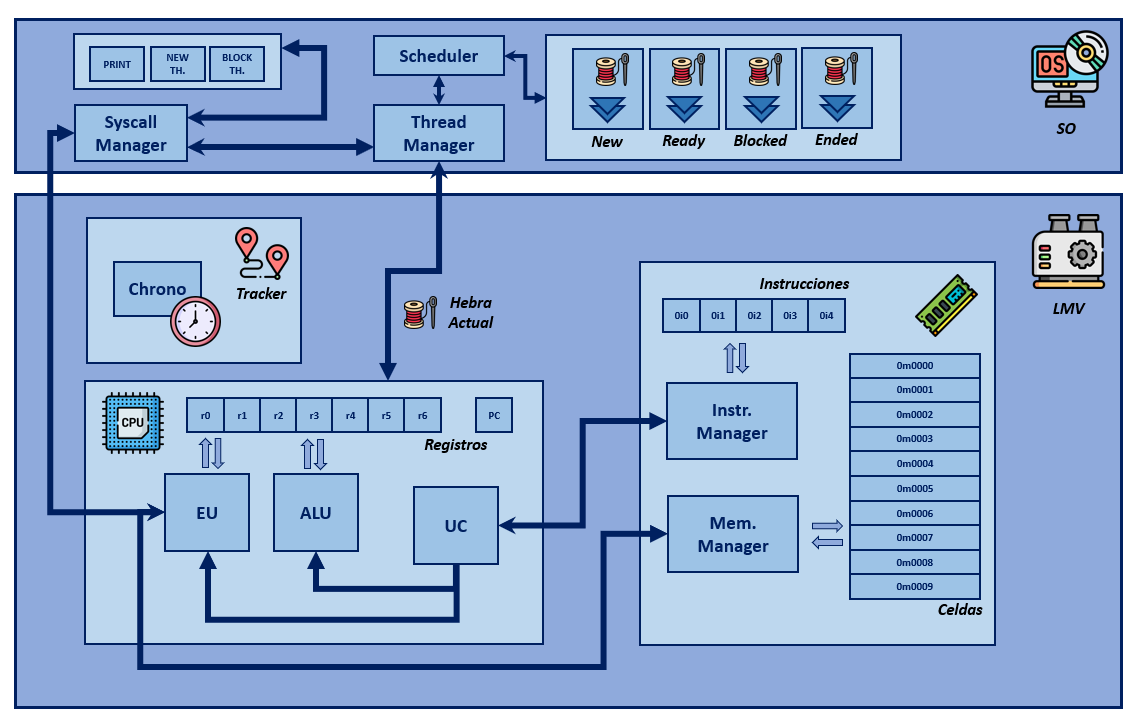
\includegraphics[width=\linewidth]{images/lmp/LVM_resume.png}
    \caption{Esquemático de la Máquina Virtual de Lamport}
    \label{fig:LVMResume}
\end{figure}

\begin{itemize}
    \item \textbf{CPU (~\ref{subsubsec:CPULVM} )}: El núcleo de procesamiento, que realiza operaciones aritméticas, lógicas y de control. Incluye un conjunto de registros, un contador de programa y una Unidad de Ejecución.
    
    \item \textbf{Memoria (~\ref{subsec:memoryLVM} )}: Almacena datos e instrucciones, optimizando el acceso y gestión de la información.

    \item \textbf{Sistema Operativo (~\ref{subsec:SOLVM} )}: Administra recursos y facilita la interacción entre software y hardware simulado.
\end{itemize}

\subsection{CPU}\label{subsubsec:CPULVM}
La CPU es responsable de ejecutar instrucciones y gestionar operaciones. Incluye un vector de registros para almacenamiento temporal, un contador de programa para seguimiento de instrucciones, una Unidad Aritmético Lógica (ALU) para operaciones matemáticas y lógicas, una Unidad de Control para coordinar actividades, y una Unidad de Ejecución para llevar a cabo instrucciones.

\subsubsection{Registros}\label{subsubsec:registrosLVM}
Los registros son de las partes más importantes de la CPU en la máquina virtual, ya que albergan y gestionan los valores que las instrucciones de operación requieren para su ejecución, principalmente para tareas de consulta y modificación. Siguiendo el esquema de registros "infinitos" discutido en ~\ref{subsec:asignacionRegIR}, la estructura del vector de registros se organiza de la siguiente manera:
\begin{itemize}
    \item \textbf{Registros r0 - r30}: Registros dedicados a parámetros y variables locales de subprogramas.
    \item \textbf{Registro r31}: Registro dedicado al retorno de una función.
    \item \textbf{Registros r32 en adelante}: Registros de propósito general.
\end{itemize}

\subsection{Esquema de ejecución de código en LVM}
Finalmente, lo que queda es comentar cómo es el esquema general de ejecución de instrucciones IR en la Máquina Virtual de Lamport:

\begin{enumerate}
    \item Creación de la tabla de segmentos y volcado de contenidos iniciales en la memoria.
    \item Iniciación de hebras correspondientes a procesos estáticos y una hebra maestra encargada de comenzar la ejecución.
    \item Decisión de qué hebra ejecuta el procesador en cada ciclo de CPU mediante un planificador.
    \item Finalización del programa cuando se alcanza \code{IR_END_PROGRAM} o todos los procesos terminan su ejecución.
\end{enumerate}

\subsection{Memoria}\label{subsec:memoryLVM}
La memoria de la LVM utiliza un mapa ordenado para simular una memoria física. Se gestiona mediante un esquema segmentado para organizar diferentes tipos de datos y facilitar la traducción de direcciones virtuales a físicas.

\subsubsection{Tabla de segmentos}\label{subsubsec:pageTableLVM}
La tabla de segmentos administra la correspondencia entre direcciones lógicas y físicas, organizando segmentos para literales, etiquetas, variables globales, índices y variables locales de procesos.


A continuación se especifican los segmentos definidos y los rangos de direcciones físicas asignados:

\begin{itemize}
    \item \textbf{Segmento 0 (literales):} Desde la dirección 0 hasta la dirección 999.
    \item \textbf{Segmento 1 (etiquetas):} Desde la dirección 1000 hasta la dirección 1999.
    \item \textbf{Segmento 2 en adelante (variable):} Desde la dirección 2000 en adelante. Aquí se definen múltiples segmentos consecutivos dependiendo de:
    \begin{itemize}
        \item Si hay variables globales (segmento 2).
        \item Si hay índices de bucles (segmento 3).
        \item Número de procesos (segmento 4 en adelante).
    \end{itemize}
\end{itemize}

\subsubsection{Iniciador de la memoria}
En la fase de generación de código intermedio, específicamente en la tabla de variables, hay un campo denominado \textit{valor inicial}. Simplemente contiene el valor de inicio de la variable en función del tipo de dato, por ejemplo 0 para los enteros, o la cadena vacía para los strings. Teniendo en cuenta esto y el esquema de segmentación implementado anteriormente, se decidió desarrollar una clase encargada de volcar a memoria todo el contenido de todas las tablas en los bloques de memoria correspondientes a las direcciones físicas.

\subsection{Sistema Operativo}\label{subsec:SOLVM}
El sistema operativo de la LVM gestiona la interacción entre software y hardware simulado. Sus responsabilidades incluyen el manejo de llamadas al sistema, coordinación de la CPU con el planificador de procesos, y gestión de bloqueo y terminación de procesos.

\subsection{Estado de la memoria de LVM con ``HolaMundo''}
Se acerca el momento en el que el programa ``HolaMundo'' (~\ref{fig:lamportHolaMundo} ) podrá ser ejecutado como un lenguaje cualquiera, pero antes de ello se muestra la fase donde el contenido de las tablas de literales, variables y etiquetas definidas en ~\ref{fig:IRHolaMundo} se vuelca a la memoria de la máquina.


\noindent
Este es el resultado de la ejecución del iniciador de memoria:
\begin{verbatim}
==========================================================
TABLA DE SEGMENTOS
==========================================================
Segmento número (0) : literales
==========================================================
Dirección Virtual    Dirección Física    
==========================================================
0                     0m00000000            
1                     0m00000001            
2                     0m00000002            
3                     0m00000003            
4                     0m00000004            
5                     0m00000005            
6                     0m00000006            
==========================================================

Segmento número (1) : etiquetas
==========================================================
Dirección Virtual    Dirección Física    
==========================================================
0                     0m00001000            
1                     0m00001001            
2                     0m00001002            
3                     0m00001003            
4                     0m00001004            
5                     0m00001005            
6                     0m00001006            
==========================================================

Segmento número (2) : variables globales
==========================================================
Dirección Virtual    Dirección Física    
==========================================================
0                     0m00002000            
==========================================================

Segmento número (3) : indices
==========================================================
Dirección Virtual    Dirección Física    
==========================================================
==========================================================

Segmento número (4) : Main
==========================================================
Dirección Virtual    Dirección Física    
==========================================================
4                     0m00002001            
5                     0m00002002            
==========================================================

==========================================================
MEMORIA DE LA MÁQUINA VIRTUAL
==========================================================
Dirección            Tipo de bloque        Contenido             
==========================================================
0m00000000            string                "Hola ""             
0m00000001            string                "!"                 
0m00000002            integer               0                     
0m00000003            integer               18                    
0m00000004            string                "Daniel"            
0m00000005            integer               23                    
0m00000006            string                "El numero magico vale: "
0m00001000            instr. address        0i0001                
0m00001001            instr. address        0i0004                
0m00001002            instr. address        0i0013                
0m00001003            instr. address        0i0014                
0m00001004            instr. address        0i0022                
0m00001005            instr. address        0i0025                
0m00001006            instr. address        0i0042                
0m00002000            integer               0                     
0m00002001            string                ""                    
0m00002002            integer               0                     
\end{verbatim}
\begin{figure}[hbtp]
\caption{Programa ``¡Hola Mundo!'' Lamport: Tabla de segmentos y memoria de LVM en su estado inicial.}
\label{fig:preLVMHolaMundo}
\end{figure}

\subsection{Control de excepciones}
Como se mencionó en ~\ref{subsec:semanticaLamport}, el lenguaje Lamport es \textit{inseguro}. Esto pone en manos del programador la responsabilidad de garantizar la corrección de ciertas operaciones. Sin las debidas precauciones, el comportamiento del programa podría ser indeterminado. Esta circunstancia destaca la necesidad de implementar un mecanismo de \textit{excepciones}.


Una excepción juega un papel crucial en la gestión de errores y situaciones inesperadas durante la ejecución de un programa. Sirve como mecanismo de señalización que indica que algo ha ido mal o que ha surgido una condición no prevista.


\noindent
La Máquina Virtual de Lamport es capaz de tratar dos tipos de excepciones:
\begin{itemize}
    \item \textbf{Excepción ZeroDivision:} Se produce cuando se intenta realizar una operación de división, cuyo segundo operando (divisor) es el número 0.
    \item \textbf{Excepción OutOfBounds:} Se produce cuando se intenta relizar un acceso indebido a un array, esto es, una posición fuera de los límites que le corresponden.
\end{itemize}

\section{Hebras y planificación}
Dado que el motivo principal de este proyecto es \textit{simular concurrencia}, se ha considerado pertinente dedicar este espacio específico para tratar en profundidad la implementación y gestión de hebras, así como el mecanismo de planificación que las coordina. A continuación, se detallan los mecanismos y estrategias adoptadas para lograr una simulación fiel y eficiente de la concurrencia en la Máquina Virtual.

\subsection{Tipos de hebras}
En la Máquina Virtual hay diferentes tipos de hebras dependiendo de su naturaleza, enumerándose a continuación:

\begin{itemize}
    \item \textbf{Iniciadora}. Es una hebra especial que se crea una única vez, al inicio del programa. Su misión es inicializar las variables globales si las hay. Acto seguido, se destruye y se empieza el ciclo de CPU con las hebras de proceso.
    \item \textbf{Estáticas}. Estas hebras son aquellas que corresponden a un proceso de Lamport y están definidas desde el inicio del programa. Su existencia y características se determinan en tiempo de traducción, y no varían durante la ejecución del programa.
    \item \textbf{Dinámicas:} Son hebras creadas en tiempo de ejecución, dependiendo del flujo y las condiciones del programa. Un claro ejemplo de la creación de una hebra dinámica es cuando se ejecuta una instrucción del tipo \code{fork}. Estas hebras ofrecen una gran flexibilidad, adaptándose a las necesidades y circunstancias que surgen durante la ejecución del programa.
\end{itemize}

\subsection{Implementación de hebras}
Cada hebra en la LVM es una unidad mínima de ejecución y se compone de varios elementos como identificador, estado, segmento de memoria, registros, pila de ejecución, contador de instrucciones, quantum, y en el caso de hebras hijas, una referencia al proceso padre.

\subsection{El modelo de 5 estados para Hebras}

El modelo de 5 estados representa un marco conceptual que permite entender y categorizar las diferentes etapas o fases por las que una hebra puede pasar durante su ciclo de vida. Cada estado ofrece una perspectiva única sobre la condición y actividad de la hebra. A continuación, se describen brevemente estos cinco estados:

\begin{enumerate}
    \item \textbf{Nuevo (New):} En este estado, la hebra ha sido creada pero aún no ha comenzado su ejecución. Está esperando la asignación de recursos necesarios para iniciar.

    \item \textbf{Listo (Ready):} La hebra está lista para ejecutarse y está esperando ser asignada a un procesador por el planificador. Todos los recursos necesarios ya han sido asignados, pero la hebra no está siendo ejecutada en este momento.

    \item \textbf{En ejecución (Running):} La hebra ha sido asignada a un procesador y está siendo ejecutada actualmente. En este estado, la hebra realiza sus tareas designadas.

    \item \textbf{Bloqueado (Blocked):} Aquí, la hebra está esperando un evento o recurso específico para continuar. Puede estar esperando la conclusión de una operación de I/O, la liberación de un recurso, o cualquier otro evento que impida su ejecución continua.

    \item \textbf{Terminado (Terminated):} La hebra ha completado su ejecución y ha finalizado todas sus tareas. Una vez que una hebra alcanza este estado, no puede regresar a los estados anteriores.
\end{enumerate}

Este modelo proporciona una estructura clara para visualizar y entender el flujo y transiciones que una hebra experimenta, facilitando la gestión y control de la concurrencia en sistemas informáticos.

\begin{figure}[h]
    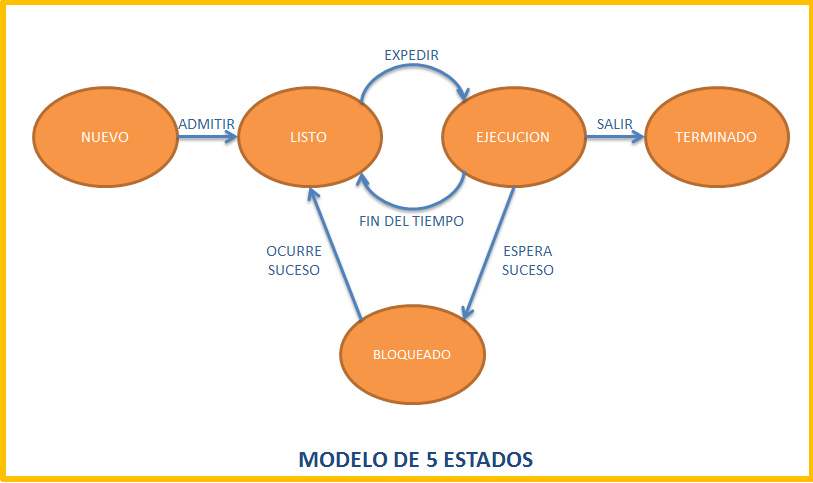
\includegraphics[width=\linewidth]{images/implementacion/hebras/modelo5_estados.png}
    \caption{Modelo de 5 estados para hebras. Diagrama de transiciones.}
    \label{fig:modelo_estados_hebras}
\end{figure}

\newpage

\subsection{Planificador. Esquema Round-Robin con Quantums aleatorios}
El esquema de planificación Round-Robin con Quantums aleatorios de la LVM introduce una variabilidad en el tiempo de ejecución asignado a cada hebra, añadiendo un factor dinámico para mejorar la eficiencia del sistema.

A continuación se explica el concepto de \textbf{quantum aleatorio}: cada hebra recibe un \textit{quantum}, definido como el número de instrucciones permitidas para ejecutar antes de ceder el CPU, que varía aleatoriamente entre 1 y 4 instrucciones. Este enfoque busca optimizar la asignación de recursos ajustándose a las condiciones del sistema.

\subsubsection{Componentes del planificador}
\noindent
El planificador, además de su algoritmo de planificación, consta de los siguientes elementos:
\begin{itemize}
    \item Una cola de hebras nuevas.
    \item Una cola de hebras listas.
    \item Una cola de hebras bloqueadas.
    \item Una cola de hebras terminadas.
    \item Un puntero a la hebra que está actualmente ejecutando.
\end{itemize}

\subsubsection{Proceso de planificación}
Finalmente, se describe el esquema de planificación Round-Robin definido para la simulación de la concurrencia entre hebras:
\begin{enumerate}
    \item \textbf{Inicialización}: Todas las hebras nuevas se mueven a la cola de listas y se elige una al azar para empezar la ejecución.
    \item \textbf{Ejecución Continua}: Si solo hay una hebra activa, controla el CPU indefinidamente.

    \item \textbf{Selección de Hebras}:
    \begin{enumerate}
        \item Si hay, se añaden hebras nuevas a la cola de listas.
        \item Si la hebra actual excede su quantum, se reubica al final de la cola de listas y se selecciona la siguiente hebra para ejecución. En caso contrario, si todavía dispone de tiempo en CPU, sigue controlándola.
        \item Si la hebra actual se encuentra ejecutando una sección atómica, continua con el control de la CPU hasta que salga. Esto se hará independientemente de si ha excedido su quantum o no.
        \item Si la hebra actual termina, se mueve a la cola de terminadas y notifica a su hebra padre si es aplicable. En ese caso, se selecciona otra hebra a ejecutar.
        \item Si la hebra actual es bloqueada, se mueve a la cola de bloqueadas y se selecciona otra hebra a ejecutar.
    \end{enumerate}

\end{enumerate}

Este esquema garantiza un balance entre equidad y eficiencia, permitiendo a las hebras compartir el CPU de manera justa y adaptativa, además de realizar una simulación más realista.

\section{Gestión de señales de interrupción UNIX (POSIX)}\label{sec:posixSignalsLMP}
En el desarrollo de la Máquina Virtual de Lamport, se ha implementado un mecanismo de gestión de señales de interrupción UNIX, siguiendo el estándar POSIX, con especial atención a la señal de interrupción Ctrl+C (SIGINT). Este mecanismo desempeña un papel crucial en la operación segura y controlada de la máquina virtual, especialmente en situaciones de bloqueo o ejecución de bucles infinitos.

La interrupción Ctrl+C es una señal común en los entornos de sistemas operativos UNIX para solicitar la terminación de un proceso en ejecución. En el contexto de la Máquina Virtual de Lamport, esta señal ha sido configurada para funcionar como un mecanismo de detención segura. Al detectar la señal de interrupción, la máquina virtual inicia un proceso de cierre ordenado, asegurando que todos los recursos y procesos en ejecución se gestionen adecuadamente antes de la terminación.

La implementación de este mecanismo de gestión de señales no solo mejora la robustez de la Máquina Virtual de Lamport, sino que también enriquece la experiencia del usuario al proporcionar una forma efectiva y segura de manejar situaciones inesperadas durante la ejecución del programa. Además, alinea la máquina virtual con las prácticas estándar en entornos UNIX, facilitando su integración y uso en estos sistemas.

\section{Interfaces de control de intérprete: ``LMP Utils``}\label{sec:implementacionLMPUtils}
Hasta ahora se han definido y desarrollado una gran cantidad de módulos que se comunican entre sí de varias formas. Es por ello por lo que es necesario establecer una vía de control de forma sencilla y unificada entre cada módulo y la función principal del intérprete que es quien ejecuta todos los analizadores y clases en el orden que corresponde. En total se han definido un total de 5 controladores diferentes:

\begin{itemize}
    \item \textbf{Controlador de flujos de E/S:} Es el encargado de realizar el tratamiento de apertura y cierre del fichero de código Lamport a ejecutar.
    \item \textbf{Controlador de Análisis:} Es el encargado de ejecutar los analizadores sintáctico y semántico, y de mantener el AST del programa, enviando al intérprete los errores en caso de que se produzcan.
    \item \textbf{Controlador de IR:} Es el encargado de llamar al optimizadador de AST y constructor de instrucciones de código intermedio.
    \item \textbf{Controlador de LVM:} Es el encargado de lanzar la máquina virtual cuando se ha generado el código intermedio.
    \item \textbf{Controlador de registros de eventos (logging):} Este controlador es especial y extremadamente útil para el usuario del intérprete. Su función es registrar todos los eventos que se han producido en el intérprete, desde el análisis sintáctico pasando a la generación de código intermedio, estado de la memoria de la LVM y traza de ejecución, o la generación de errores.

    Genera un directorio denominado \code{log/} que contiene los ficheros de logging siguientes:
    \begin{itemize}
        \item \textbf{logging de AST}: Contiene el AST generado para el programa.
        \item \textbf{logging de IR}: Contiene las tablas de literales, variables y etiquetas, y el listado de instrucciones IR.
        \item \textbf{logging de LVM}: Contiene la tabla de segmentos y el estado de la memoria en el inicio de la máquina lamport, además de la traza de ejecución de la máquina al terminar. Además, también genera un fichero de registro con toda la traza de ejecución del programa en la Máquina Virtual.
        \item \textbf{logging de errores}: Contiene el listado de errores producidos en el análisis.
    \end{itemize}
\end{itemize}

\section{Ejecución de ``HolaMundo''}
Se ha llegado al final del proyecto, donde por fin se puede ejecutar el programa ``HolaMundo'' (~\ref{fig:lamportHolaMundo} ) del que tantas veces se ha hablado a lo largo de estas secciones. 


\noindent
El resultado de la ejecución es el siguiente:
\begin{figure}[h]
  \begin{minipage}{\linewidth}
    \centering
    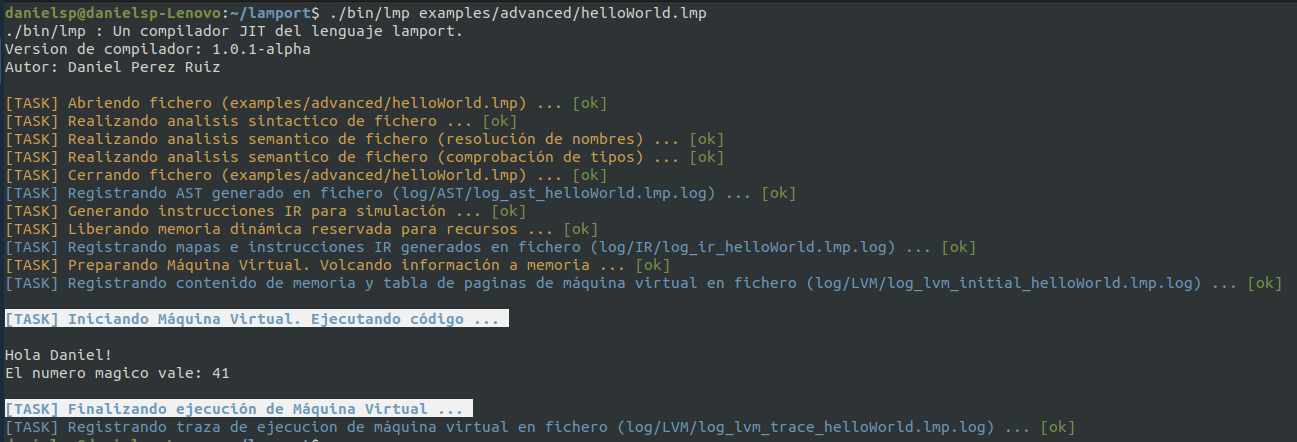
\includegraphics[width=\linewidth]{images/implementacion/ejecucion/lmp_hola_mundo.png}
    \caption{Ejecución de ``HolaMundo'' en el compilador.}
    \label{fig:ejecucionHolaMundo}
  \end{minipage}
  \vspace{10pt} 
  \begin{minipage}{\linewidth}
    \centering
    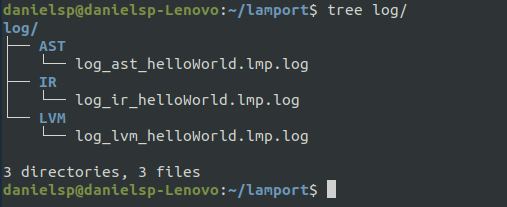
\includegraphics[width=\linewidth]{images/implementacion/ejecucion/logs.png}
    \caption{Ficheros de logging generados tras la ejecución.}
    \label{fig:logsHolaMundo}
  \end{minipage}
\end{figure}

\newpage
\subsection{Traza de ejecución de ``HolaMundo''}
Al finalizar la máquina virtual, se genera un fichero de registro con todas las operaciones que ésta ha ido realizando a nivel de CPU y de memoria. En la siguiente imagen se muestra la cabecera de la traza de ejecución para el programa ``HolaMundo'':
\begin{figure}[h]
  \begin{minipage}{\linewidth}
    \centering
    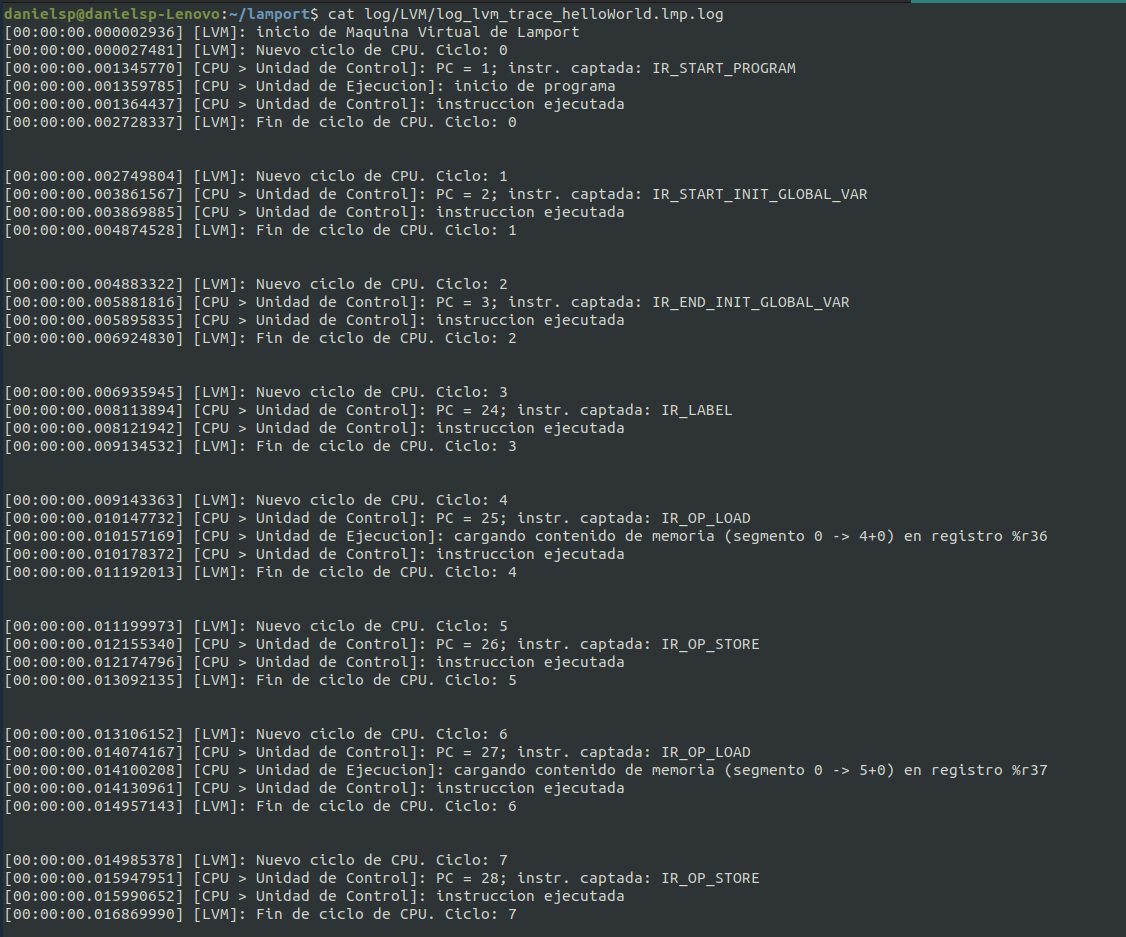
\includegraphics[width=\linewidth]{images/implementacion/ejecucion/resumed_traza.png}
    \caption{Traza de ejecución de ``HolaMundo''.}
    \label{fig:trazaHolaMundo}
  \end{minipage}
\end{figure}

\newpage
\section{Dockerización del intérprete}
Con la evolución constante de la tecnología y las infraestructuras de software, la necesidad de crear aplicaciones portables y escalables ha cobrado mayor importancia. Docker, una herramienta que permite la creación de contenedores, surge como una solución a esta demanda. Un contenedor Docker encapsula una aplicación junto con todas sus dependencias en una unidad estándar de software, garantizando que la aplicación se ejecute de la misma manera sin importar dónde se despliegue. 



En el contexto del intérprete desarrollado, la dockerización ofrece ventajas significativas en términos de portabilidad, aislamiento y replicabilidad. Esta sección detallará el proceso y las consideraciones adoptadas al dockerizar el intérprete, permitiendo su distribución y ejecución de manera homogénea en diferentes entornos.

\subsection{Construcción del contenedor}
Para construir el contenedor Docker que encapsulará el intérprete junto con todas sus dependencias, se han realizado las siguientes tareas:

\begin{enumerate}
    \item Elección de una imagen base. Ésta debe ser del menor tamaño posible para que sólo contenga lo imprescindible, además de ser una imagen que reciba constantes actualizaciones de seguridad y mantenimiento. En el caso de este proyecto, \textbf{alpine} es una excelente elección por cumplir estas dos características.
    \item Construir el fichero \code{Dockerfile}. Este fichero indica cómo se debe construir el contenedor de forma automática, aprovisionándolo de todas las dependencias.
    \item Definir script de ejecución utilizando el contenedor virtual. Para hacer aún más fácil el uso de esta herramienta se definió un script denominado \code{./lmp_docker.sh} que ejecuta el contenedor utilizando como argumento el fichero de código Lamport indicado.
\end{enumerate}

\subsection{Compilación estática del intérprete}
La compilación estática se refiere al proceso de integrar todas las bibliotecas y dependencias requeridas por una aplicación directamente en el binario ejecutable, en lugar de depender de bibliotecas compartidas en el sistema en tiempo de ejecución. Este método tiene varias ventajas, especialmente en el contexto que concierne a esta sección:

\begin{itemize}
\item \textbf{Portabilidad mejorada}: Un binario estáticamente enlazado no tiene dependencias externas, lo que garantiza que funcionará en cualquier entorno que lo ejecute, eliminando así problemas relacionados con versiones de bibliotecas o dependencias faltantes.
\item \textbf{Reducción del tamaño del contenedor}: Al no requerir la instalación de bibliotecas adicionales en el contenedor (sólo se necesita instalar flex y bison de manera inevitable), el tamaño de la imagen resultante puede reducirse significativamente. En este proyecto, la imagen del contenedor se redujo de 249 MB a tan solo 24 MB, una optimización impresionante.
\item \textbf{Seguridad mejorada}: Al reducir el número de componentes en el contenedor, se disminuye la superficie de ataque potencial, al eliminar software adicional que no es esencial para la aplicación pero que podría presentar vulnerabilidades.
\end{itemize}

Para lograr la compilación estática del intérprete, se utilizaron las herramientas gcc y g++ con las opciones de enlazado estático. Además, se aprovechó el enfoque de construcción multi-etapa en Docker, donde la primera etapa incluye todas las herramientas y dependencias necesarias para la compilación, y la segunda etapa simplemente copia el binario resultante, resultando en una imagen Docker final limpia y optimizada.

\begin{figure}[h]
    \begin{adjustbox}{center}
        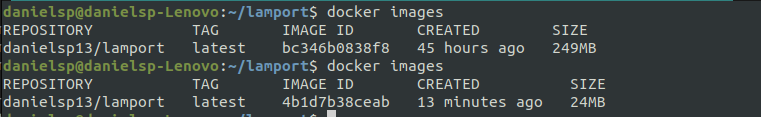
\includegraphics[width=\linewidth]{images/implementacion/docker/docker_reduce.png}
    \end{adjustbox}
    \caption{Tamaño de contenedor docker antes y después de usar compilación estática.}
    \label{fig:DockerReduce}
\end{figure}
	\chapter{\textbf{Programas escritos en Lamport}}
En este capítulo se definen algunos ejemplos de programas escritos en el lenguaje Lamport y su resultado de ejecución, con el objetivo de mostrar el correcto funcionamiento del compilador:

\section{Ejemplos secuenciales}
Los siguientes ejemplos mostrados aquí no necesitan de concurrencia para funcionar, pues siguen la estructura y sintaxis básica de cualquier otro programa desarrollado en cualquier lenguaje de alto nivel convencional:

\subsection{Ejemplo 1: Operaciones aritméticas}
\begin{lstlisting}[style=lamportStyle]
{Programa: arithmetic_operations.lmp}
{Autor: Daniel Perez Ruiz}

program Operaciones;
	var num1 : integer := (-4 + 6) * 10 - 2;
	var num2 : real := 3.0;

process Main;
	var num3 : integer := 5;
	var num4 : real := (3.5 * 4.2) + (6.7 - 2.3) / 1.1;
begin
	print("num1 tiene de valor: ",num1);
	print("num3 tiene de valor: ",num3);
	print("");
	
	print("num1 + num3 = ",num1+num3);
	print("num1 - num3 = ",num1-num3);
	print("num1 * num3 = ",num1*num3);
	print("num1 / num3 = ",num1/num3);
	print("num1 % num3 = ",num1%num3);
	print("-num1 = ",-num1);
	
	print("");
	
	print("num2 tiene de valor: ",num2);
	print("num4 tiene de valor: ",num4);	
	print("");
	
	print("num2 + num4 = ",num2+num4);
	print("num2 - num4 = ",num2-num4);
	print("num2 * num4 = ",num2*num4);
	print("num2 / num4 = ",num2/num4);
	print("-num4 = ",-num4);
	
end
\end{lstlisting}
\begin{figure}[h]
\caption{Programa Lamport: operaciones aritméticas}
\label{fig:lamportArithmeticOperations}
\end{figure}

\newpage
\begin{figure}[h]
    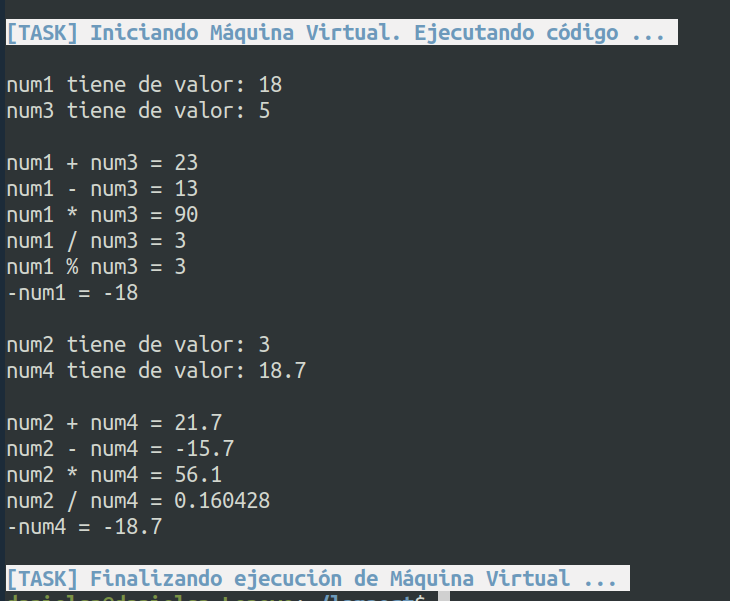
\includegraphics[width=\linewidth]{images/ejemplos/arithmeticOperations.png}
    \caption{Ejecución de programa: operaciones aritméticas.}
    \label{fig:lamportArithmeticOperations_exec}
\end{figure}

\newpage
\subsection{Ejemplo 2: Operaciones lógicas}
\begin{lstlisting}[style=lamportStyle]
{Programa: logical_operations.lmp}
{Autor: Daniel Perez Ruiz}

program Operaciones;
	var a : boolean := true;
	var b : boolean := false;

process Main;
	var c : boolean := true;
begin
	print("a es: ",a);
	print("b es: ",b);
	print("c es: ",c);
	print("");
	
	print("a y b es: ",a and b);
	print("a y c es: ",a and c);
	print("a y b y c es: ",a and b and c);
	print("");
	
	print("a o b es: ",a or b);
	print("a o c es: ",a or c);
	print("a o b o c es: ",a or b or c);
	print("");
	
	print("(a o b) y c es: ", (a or b) and c);
	print("(a o c) y b es: ", (a or c) and b);
	print("");
	
	print("no a es: ",not a);
	print("no b es: ",not b);
	
end
\end{lstlisting}
\begin{figure}[h]
\caption{Programa Lamport: operaciones lógicas}
\label{fig:lamportLogicalOperations}
\end{figure}

\newpage
\begin{figure}[h]
    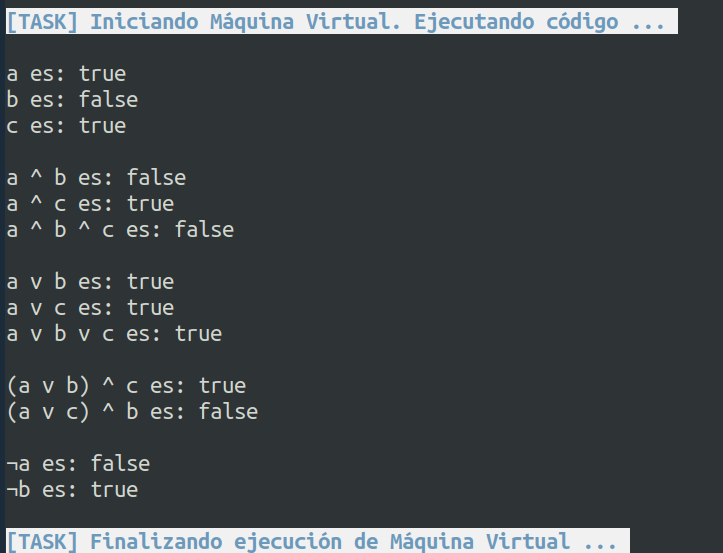
\includegraphics[width=\linewidth]{images/ejemplos/logical_operations.png}
    \caption{Ejecución de programa: operaciones lógicas.}
    \label{fig:lamportLogicalOperations_exec}
\end{figure}

\newpage
\subsection{Ejemplo 3: If/Else}
\begin{lstlisting}[style=lamportStyle]
{Programa: ifelse.lmp}
{Autor: Daniel Perez Ruiz}

program CompruebaEdad;
	var nombre1 : string := "Jorge";
	var edad1 : integer := 17;
	
	var nombre2 : string := "Pablo";
	var edad2 : integer := 22;
	
process main;
	var minimaEdad : integer := 18;
begin
	print(nombre1, ", tu edad es: ",edad1,". Comprobando si puedes entrar...");
	
	if edad1 < minimaEdad then
		begin
			print("NO puedes entrar. Debes tener ",minimaEdad," para poder entrar.");
		end
	else
		begin
			print("Adelante!!. Puedes entrar");
		end
		
	print("");
		
	print(nombre2, ", tu edad es: ",edad2,". Comprobando si puedes entrar...");
	
	if edad2 < minimaEdad then
		begin
			print("NO puedes entrar. Debes tener ",minimaEdad," para poder entrar.");
		end
	else
		begin
			print("Adelante!!. Puedes entrar");
		end
end
\end{lstlisting}
\begin{figure}[h]
\caption{Programa Lamport: flujos de control if/else.}
\label{fig:lamportIfElse}
\end{figure}

\newpage
\begin{figure}[h]
    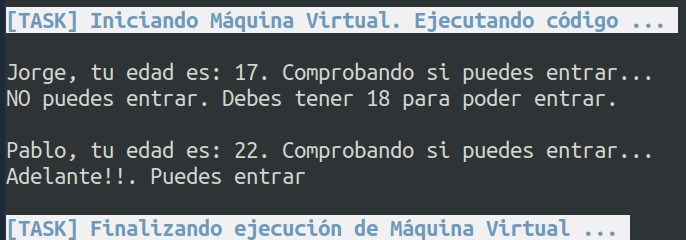
\includegraphics[width=\linewidth]{images/ejemplos/if_else.png}
    \caption{Ejecución de programa: if/else.}
    \label{fig:lamportIfElse_exec}
\end{figure}

\newpage
\subsection{Ejemplo 4: For}
\begin{lstlisting}[style=lamportStyle]
{Programa: for.lmp}
{Autor: Daniel Perez Ruiz}

program Bucles
	var contador : integer := 5;

process main;
	var startFor : integer := 1;
	var endFor : integer := 5;
begin
	print("La variable contador empieza en: ",contador);
	print("");
	print("Bucle for empieza en: ",startFor);
	print("Bucle for acaba en: ",endFor);
	
	print("");
	
	for i := startFor to endFor do
	begin
		contador := contador+1;
		print("--- contador vale ahora: ",contador);
		print("--- i vale: ", i);
	end
	
	print("");
	print("Ejecutando bucles anidados ...");
	print("");
	
	for j := 1 to 3 do
	begin
		print("------ j vale: ",j);
		for k := j to 4 do
		begin
			print("--- k vale: ",k);
		end
		print("");
	end
	
end
\end{lstlisting}
\begin{figure}[h]
\caption{Programa Lamport: bucles for.}
\label{fig:lamportFor}
\end{figure}

\newpage
\begin{figure}[!h]
    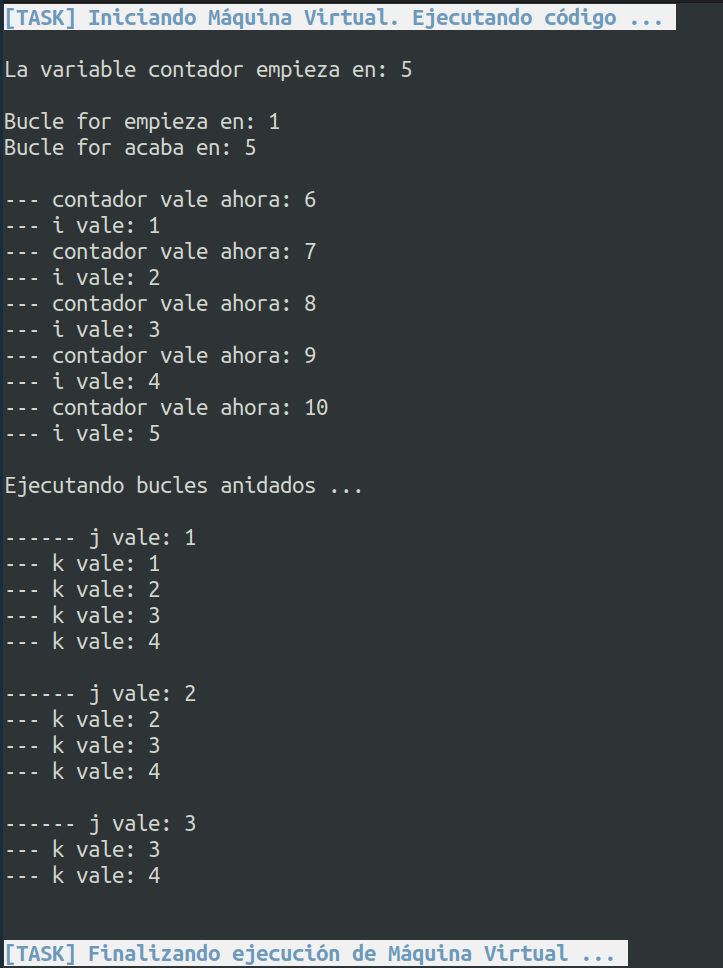
\includegraphics[scale=0.5]{images/ejemplos/for.png}
    \caption{Ejecución de programa: bucles for.}
    \label{fig:lamportFor_exec}
\end{figure}

\newpage
\subsection{Ejemplo 5: While}
\begin{lstlisting}[style=lamportStyle]
{Programa: while.lmp}
{Autor: Daniel Perez Ruiz}

program Bucles
	var contador : integer := 5;

process main;
	var valorMaximo : integer := 10;
begin
	print("La variable contador empieza en: ",contador);
	print("Su valor maximo debe ser: ",valorMaximo);
	print("");
	
	while contador < valorMaximo do
	begin
		contador := contador + 1;
		print(" --- Contador vale ahora: ", contador);
	end
	
	print(""); print("Fin de bucle");
end
\end{lstlisting}
\begin{figure}[h]
\caption{Programa Lamport: bucles while.}
\label{fig:lamportWhile}
\end{figure}

\newpage
\begin{figure}[h]
    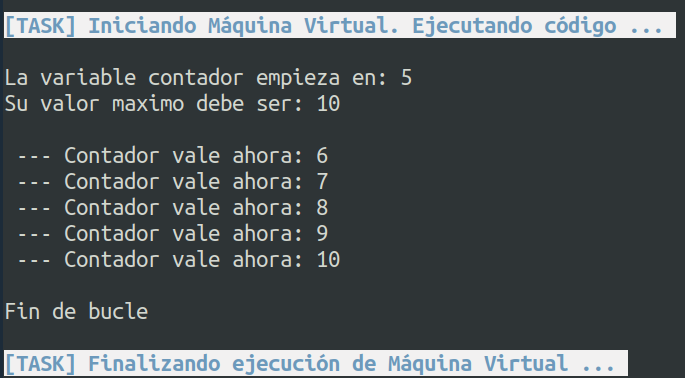
\includegraphics[width=\linewidth]{images/ejemplos/while.png}
    \caption{Ejecución de programa: bucles while.}
    \label{fig:lamportWhile_exec}
\end{figure}

\newpage
\subsection{Ejemplo 6: Uso de arrays}
\begin{lstlisting}[style=lamportStyle]
{Programa: for.lmp}
{Autor: Daniel Perez Ruiz}

program Arrays
	var numeros : array [5] integer;
process main;
	var letras : array [3] char;
begin
	print("Asignando numeros pares a array de numeros...");
	for i := 0 to 4 do
	begin
		print("Asignando a numeros[",i,"] el valor ",2*i);
		numeros[i] := 2*i;
	end
	
	print("");
	print("Imprimiendo array de numeros...");
	for j := 0 to 4 do
	begin
		print("numeros[",j,"] = ",numeros[j]);
	end
	
	letras[1] := 'd';
	print("");
	print("letras[1] es : ",letras[1]);
end
\end{lstlisting}
\begin{figure}[h]
\caption{Programa Lamport: uso de arrays}
\label{fig:lamportArray}
\end{figure}

\newpage
\begin{figure}[h]
    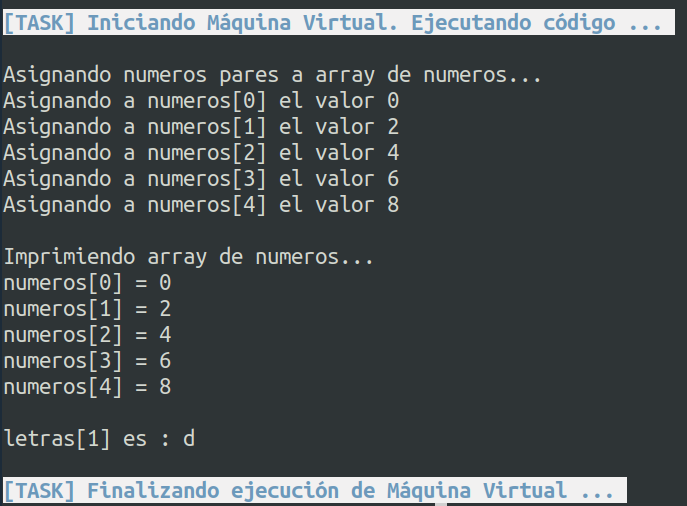
\includegraphics[width=\linewidth]{images/ejemplos/array.png}
    \caption{Ejecución de programa: arrays.}
    \label{fig:lamportArray_exec}
\end{figure}

\section{Ejemplos concurrentes}
Para finalizar, ha llegado el momento de verificar si se ha solucionado el problema que se planteó en el capítulo ~\ref{chapter:problema}, que es el de \textit{disponer de un lenguaje que permita simular sistemas concurrentes}. A continuación, se presenta una serie de ejemplos detallados que requiere de uso de concurrencia en el compilador:

\subsection{Ejemplo 1: Múltiples procesos estáticos}
En este ejemplo se dispone de 3 procesos estáticos cuyo propósito es imprimir un mensaje por pantalla que consta de dos elementos: un mensaje de saludo seguido de una variable entera que actúa a modo de identificador de proceso. Estos mensajes están dentro de un bucle infinito, por lo que cada proceso se ejecutará indefinidamente:
\begin{lstlisting}[style=lamportStyle]
{Programa: race_condition.lmp}
{Autor: Daniel Perez Ruiz}

program Race

process P1;
	var id : integer := 1;
begin
	while true do
	begin
		print("te saluda el proceso: ",id);
	end
end

process P2;
	var id : integer := 2;
begin
	while true do
	begin
		print("te saluda el proceso: ",id);
	end
end

process P3;
	var id : integer := 3;
begin
	while true do
	begin
		print("te saluda el proceso: ",id);
	end
end
\end{lstlisting}
\begin{figure}[h]
\caption{Programa Lamport: múltiples procesos estáticos (race condition)}
\label{fig:lamportMultipleProcess}
\end{figure}

\begin{figure}[h]
    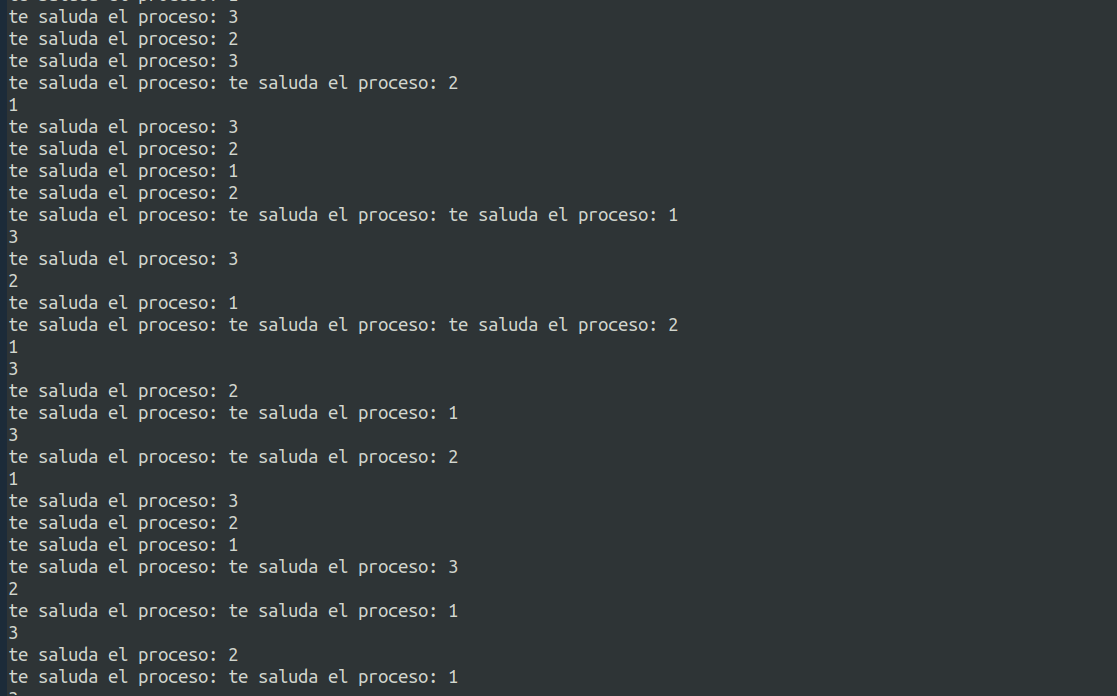
\includegraphics[width=\linewidth]{images/ejemplos/concurrentes/multiple_process.png}
    \caption{Ejecución de programa: múltiples procesos estáticos (race condition).}
    \label{fig:lamportMultipleProcess_exec}
\end{figure}

Se puede apreciar que efectivamente los tres procesos muestran mensajes. Sin embargo, en algunas ocasiones no se muestran correctamente porque se entrelazan las instrucciones de impresión de unos procesos con otros.

\newpage

\subsection{Ejemplo 2: Múltiples procesos estáticos (con sección atómica)}
Para solucionar el problema anterior, se puede introducir un bloque de secciones atómicas que contengan a las instrucciones de impresión en cada proceso, como se muestra a continuación:
\begin{lstlisting}[style=lamportStyle]
{Programa: atomic.lmp}
{Autor: Daniel Perez Ruiz}

program NotARace

process P1;
	var id : integer := 1;
begin
	while true do
	begin
		<< print("te saluda el proceso: ",id); >>
	end
end

process P2;
	var id : integer := 2;
begin
	while true do
	begin
		<< print("te saluda el proceso: ",id); >>
	end
end

process P3;
	var id : integer := 3;
begin
	while true do
	begin
		<< print("te saluda el proceso: ",id); >>
	end
end
\end{lstlisting}
\begin{figure}[h]
\caption{Programa Lamport: múltiples procesos estáticos (con sección atómica)}
\label{fig:lamportMultipleProcessAtomic}
\end{figure}

\newpage
\begin{figure}[h]
    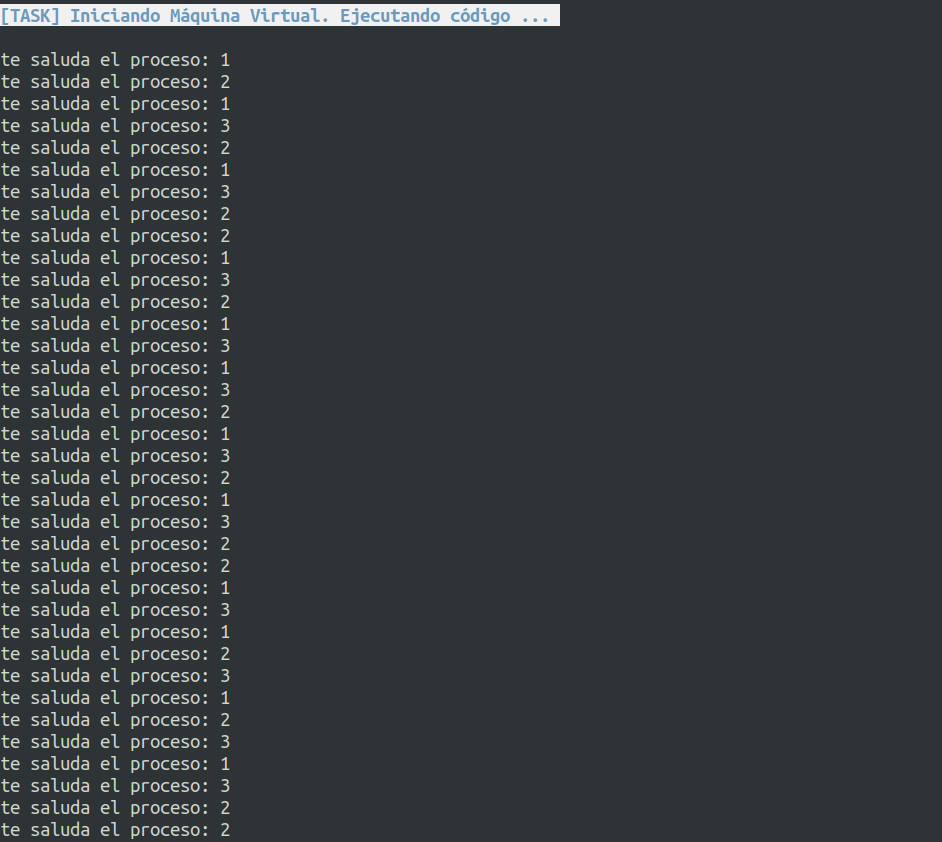
\includegraphics[width=\linewidth]{images/ejemplos/concurrentes/multiple_process_atomic.png}
    \caption{Ejecución de programa: múltiples procesos estáticos (con sección atómica)}
    \label{fig:lamportMultipleProcessAtomic_exec}
\end{figure}

Ahora, los tres procesos también muestran mensajes, pero se muestran ordenadamente debido a que, cuando una hebra entra en una sección atómica, se ejecutan todas las instrucciones que contiene hasta que termina. En este caso, se ejecutan 3 instrucciones dentro de cada sección atómica: saludo, índice y salto de línea.

\newpage
\subsection{Ejemplo 3: Vector de procesos estáticos}
En este ejemplo también se dispone de 3 procesos, pero han sido definidos mediante un vector indexado. Cada proceso dispone de su propio valor de índice, y lo utilizará para incrementar una variable compartida a los 3 procesos denominada \code{total}. El valor esperado final de la variable total es 6.
\begin{lstlisting}[style=lamportStyle]
{Programa: process_vector.lmp}
{Autor: Daniel Perez Ruiz}

program SumaIndice

	var total : integer := 0;

process VectorProc[index: 1..3];
begin
    total := total + index;
   	print("proceso (",index,") incrementa total a: ", total);
end
\end{lstlisting}
\begin{figure}[h]
\caption{Programa Lamport: vector de procesos estáticos (race condition).}
\label{fig:lamportProcessVector}
\end{figure}

\begin{figure}[h]
    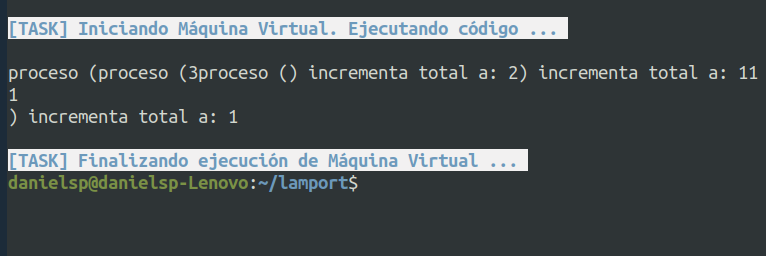
\includegraphics[width=\linewidth]{images/ejemplos/concurrentes/vector_process.png}
    \caption{Ejecución de programa: vector de procesos estáticos (race condition).}
    \label{fig:lamportProcessVector_exec}
\end{figure}

El resultado de esta ejecución es un caos tremendo debido a la concurrencia. No sólo en cuanto al contenido de los mensajes sino también en el resultado final que debería tener la variable global \code{total}.

Para solucionar el problema del ejemplo anterior es suficiente con definir una sección atómica que englobe a las dos instrucciones de los procesos. Aunque el orden de ejecución de los procesos puede ser diferente cada vez que se ejecute el programa, gracias a la sección atómica definida cada proceso muestra claramente el mensaje, y siempre el último mostrará que el resultado de la variable \code{total} es 6, como se esperaba. Esto es lo que se muestra en la figura ~\ref{fig:lamportProcessVectorAtomic_exec}.

\begin{figure}[h]
    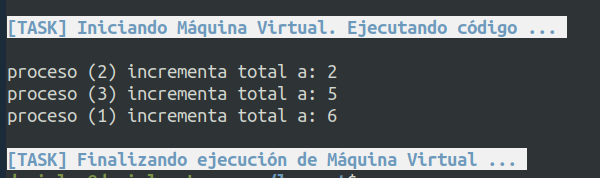
\includegraphics[width=\linewidth]{images/ejemplos/concurrentes/vector_process_atomic.png}
    \caption{Programa Lamport: vector de procesos estáticos (atómico).}
    \label{fig:lamportProcessVectorAtomic_exec}
\end{figure}



\newpage
\subsection{Ejemplo 5: Bloque de instrucciones concurrentes (cobegin-coend)}
En el siguiente ejemplo se define una variable global denominada \code{x} cuyo valor inicial es 0. Después se define un proceso \code{Main} que contiene dos instrucciones de impresión y un bloque de instrucciones concurrentes. Puesto que al igual que en los otros ejemplos presentados aquí no se ha definido ningún mecanismo de sincronización, el resultado final de la variable \code{x} puede ser impredecible, aunque lo deseable sería que fuese 0.
\begin{lstlisting}[style=lamportStyle]
{Programa: cobegin.lmp}
{Autor: Daniel Perez Ruiz}

program Cobegin
	var x : integer := 0;
	
process Main;
begin
	print("iniciando bloque cobegin ...");

	cobegin
		x := x+1;
		x := x-1;
	coend
	
	print("x vale: ",x);
end
\end{lstlisting}
\begin{figure}[h]
\caption{Programa Lamport: bloque de instrucciones concurrentes cobegin-coend (race condition).}
\label{fig:lamportCobegin}
\end{figure}

\newpage

\begin{figure}[h]
    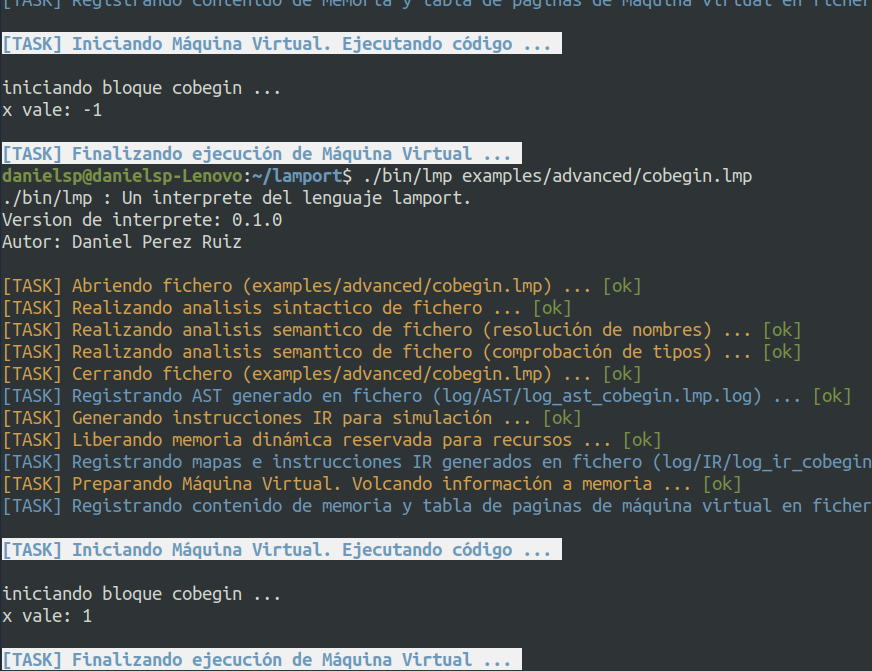
\includegraphics[width=\linewidth]{images/ejemplos/concurrentes/cobegin.png}
    \caption{Ejecución de programa: bloque de instrucciones concurrentes cobegin-coend (race condition).}
    \label{fig:lamportCobegin_exec}
\end{figure}

En estas dos ejecuciones del programa se ha obtenido un valor diferente: 1 y -1. De hecho, el conjunto de valores posibles para la variable \code{x} es: -1,0,1. Esto es evidentemente causado por el entrelazamiento de las hebras.

\vspace{0.5cm}
Notar además que, cuando se entra en un bloque cobegin, el proceso \code{Main} espera de manera implícita a que se ejecuten todas las hebras creadas dinámicamente para ejecutar todas las instrucciones que contiene.

\newpage
\subsection{Ejemplo 6: Bloque de instrucciones concurrentes (cobegin-coend) (con atomic)}
Si incluimos cada instrucción del bloque cobegin-coend en un bloque atómico, se soluciona el problema anteriormente mencionado.
\begin{lstlisting}[style=lamportStyle]
{Programa: cobegin.lmp}
{Autor: Daniel Perez Ruiz}

program Cobegin
	var x : integer := 0;
	
process Main;
begin
	print("iniciando bloque cobegin ...");

	cobegin
		<< x := x+1; >>
		<< x := x-1; >>
	coend
	
	print("x vale: ",x);
end
\end{lstlisting}
\begin{figure}[h]
\caption{Programa Lamport: bloque de instrucciones concurrentes cobegin-coend (atómico).}
\label{fig:lamportCobeginAtomic}
\end{figure}

\newpage

\begin{figure}[h]
    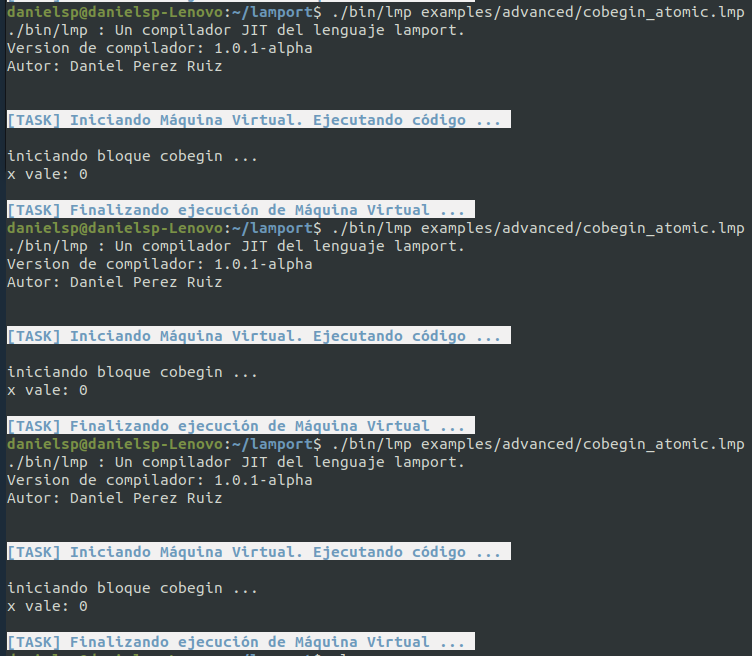
\includegraphics[width=\linewidth]{images/ejemplos/concurrentes/cobegin_atomic.png}
    \caption{Ejecución de programa: bloque de instrucciones concurrentes cobegin-coend (atómico).}
    \label{fig:lamportCobeginAtomic_exec}
\end{figure}

Ahora siempre que se ejecute este programa el resultado obtenido será 0, verificando así la buena sincronización de las hebras dentro de un bloque de instrucciones concurrentes de este tipo.

\newpage
\subsection{Ejemplo 7: Ejecución y sincronización de procedimientos concurrentes con fork-join}
En este ejemplo disponemos de una variable global \code{x} y dos procedimientos que hacen dos tareas diferentes. Uno incrementa la variable \code{x} unas 100 veces, y otro lo decrementa unas 20 veces. El resultado final que debería tener la variable es \code{x = 80}. Ejecutándolo secuencialmente, se verifica sin problema, pero el objetivo de este programa es ejecutar sendos procedimientos concurrentemente. 

\vspace{0.5cm}

El proceso \code{Main} indica a Increment que se ejecute concurrentemente con la llamada que realiza después a decrement, utilizando la sentencia \code{fork}. Con la sentencia \code{join}, la hebra \code{Main} se bloquea esperando a que \code{Increment()} termine su ejecución.
\begin{lstlisting}[style=lamportStyle]
{Programa: fork_join.lmp}
{Autor: Daniel Perez Ruiz}

program Fork;
	var x : integer := 0;

procedure Increment();
begin
	for i := 1 to 100 do
	begin
		x := x+1;
	end
	
	print("fin de increment");
end

procedure Decrement();
begin
	for j := 1 to 20 do
	begin
		x := x-1;
	end
	
	print("fin de decrement");
end

process Main;
begin
	print("Realizando fork...");
	fork Increment;
	Decrement();
	join;
	
	print("x vale: ",x);
	
	
	if(x == 80) then
	begin
		print("Se ha obtenido 80, el valor esperado");
	end
	else
	begin
		print("No se ha obtenido 80.");
	end
end
\end{lstlisting}
\begin{figure}[h]
\caption{Programa Lamport: creación y sincronización de hebras dinámicas con fork-join.}
\label{fig:lamportForkJoin}
\end{figure}

\newpage

\begin{figure}[h]
    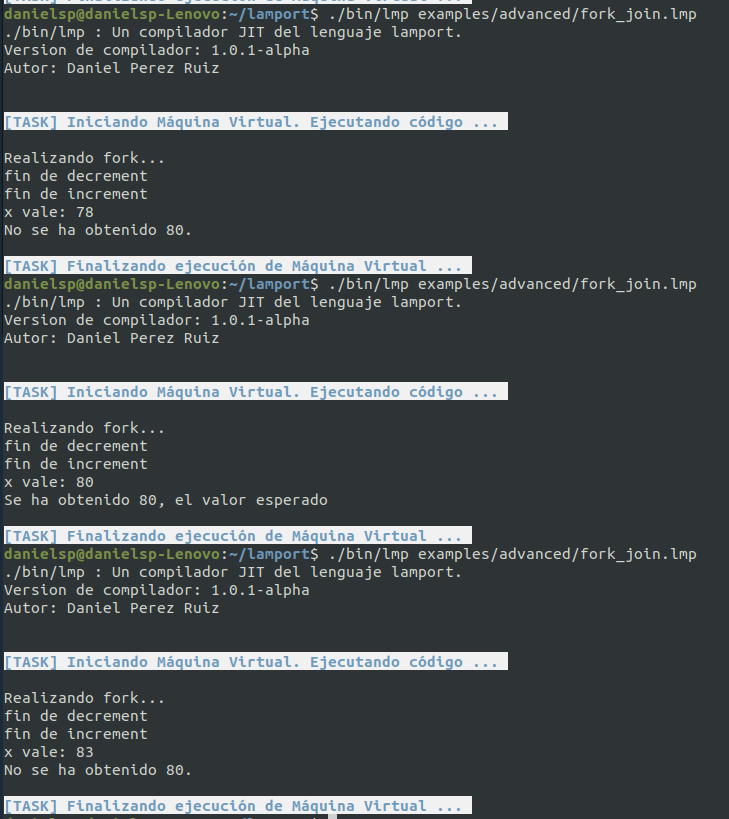
\includegraphics[width=0.88\linewidth]{images/ejemplos/concurrentes/fork_join.png}
    \caption{Ejecución de programa: creación y sincronización de hebras dinámicas con fork-join.}
    \label{fig:lamportForkJoin_exec}
\end{figure}

Se observa que la sincronización de Increment con la hebra principal Main se realiza adecuadamente, pues los mensajes que se escribieron después de join se ejecutan sí y sólo sí cuando este procedimiento ha terminado. Sin embargo, se vuelve a apreciar que en dos ejecuciones del programa no hay el resultado esperado, obteniendo dos resultados diferentes.

\newpage
Si las instrucciones de las líneas 11 y 21 se engloban dentro de una sección atómica, el resultado de la ejecución del programa es el siguiente, donde siempre se conseguirá el valor deseado de la variable \code{x}.

\begin{figure}[h]
    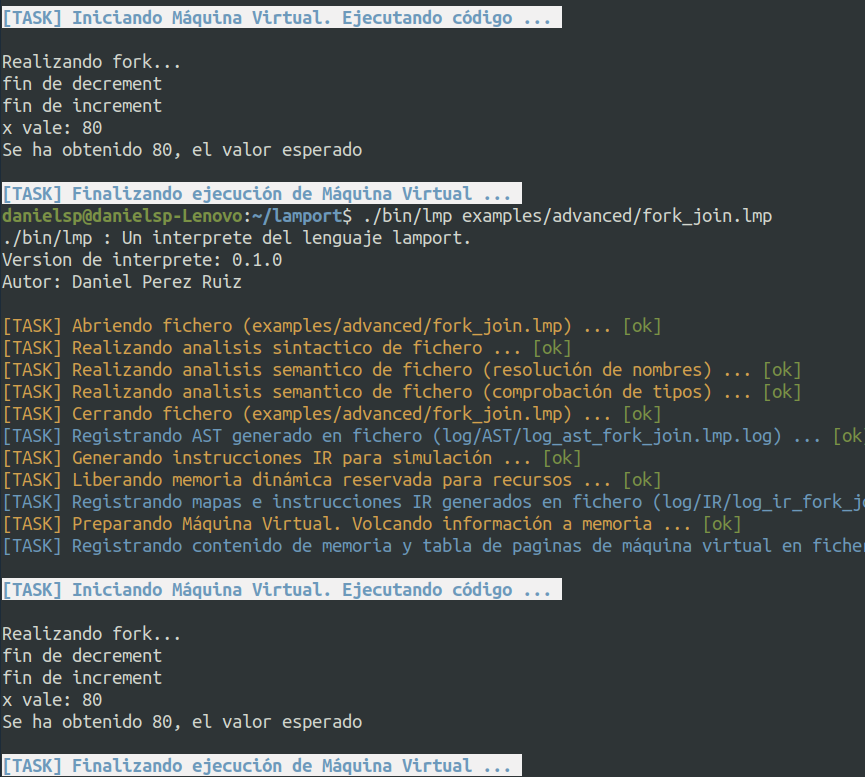
\includegraphics[width=\linewidth]{images/ejemplos/concurrentes/fork_join_atomic.png}
    \caption{Ejecución de programa: creación y sincronización de hebras dinámicas con fork-join (atómico).}
    \label{fig:lamportForkJoinAtomic_exec}
\end{figure}

\newpage
Finalmente, queda preguntarse qué sucede si se elimina la instrucción \code{join} (línea 32) que es quien sincroniza al proceso \code{Main} con su hija. Lo más probable es que lo que ocurra sea que la hebra principal termine antes que su hija, un comportamiento poco deseado y que se aprecia a continuación:

\begin{figure}[h]
    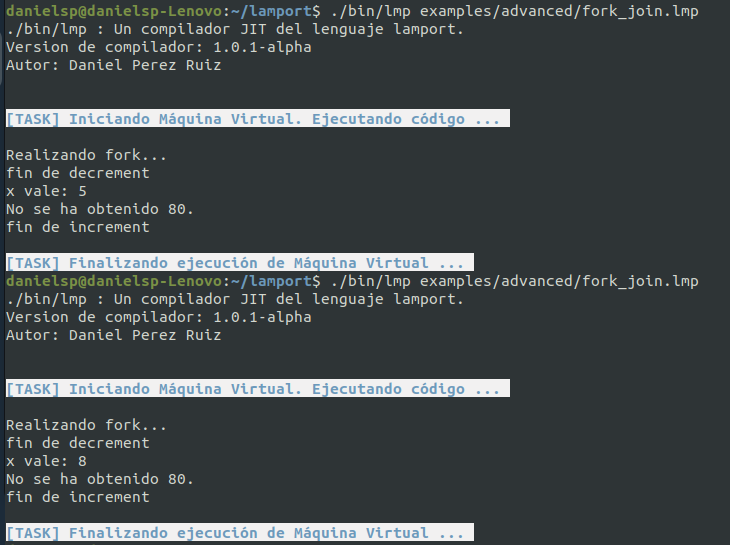
\includegraphics[width=\linewidth]{images/ejemplos/concurrentes/fork_without_join.png}
    \caption{Ejecución de programa: creación y sincronización de hebras dinámicas con fork (sin join).}
    \label{fig:lamportForkWithoutJoin_exec}
\end{figure}

Se observa que los mensajes de impresión después de la llamada a los procedimientos se muestran antes de que Increment notifique que ha terminado.

\newpage
\subsection{Ejemplo 8: Sincronización de procedimientos concurrentes con semáforos}
Este ejemplo es bastante parecido al anterior, con la salvedad de que se tiene otra forma diferente de sincronizar los procedimientos \code{Increment} y \code{Decrement}. Se observa un semáforo denominado \code{sem} y cuyo valor de inicio es 1.

\vspace{0.5cm}

Un semáforo es una herramienta de sincronización utilizada en la programación concurrente para controlar el acceso a un recurso compartido. Funciona como un contador, y sus operaciones fundamentales son \code{WAIT} (o también llamada \textit{P}) y \code{SIGNAL} (o \textit{V}). El \code{WAIT} disminuye el contador y, si este es negativo, bloquea el proceso; mientras que el \code{SIGNAL} incrementa el contador y, si hay procesos bloqueados, permite que uno de ellos continue su ejecución. De esta manera, los semáforos pueden garantizar que ciertas secciones de código no sean ejecutadas por más de un proceso a la vez, evitando condiciones de carrera y otros problemas relacionados con la concurrencia.

\begin{lstlisting}[style=lamportStyle]
{Programa: semaphore.lmp}
{Autor: Daniel Perez Ruiz}
program Semaphore;
    var x : integer := 2;
    var sem : semaphore := 1;

procedure Increment();
begin
    for i := 1 to 5 do
    begin
        WAIT sem;
        print("Incrementando x, que vale ahora: ", x);
        x := x + 1;
        SIGNAL sem;
    end
end

procedure Decrement();
begin
    for i := 1 to 5 do
    begin
        WAIT sem;
        print("Decrementando x, que vale ahora: ", x);
        x := x - 1;
        SIGNAL sem;
    end
end

process Main;
begin
    fork Increment;
    fork Decrement;
    join;
    print("x vale: ", x);
end
\end{lstlisting}
\begin{figure}[h]
\caption{Programa Lamport: sincronización de procesos con semáforo.}
\label{fig:lamportSemaphore}
\end{figure}

\begin{figure}[h]
    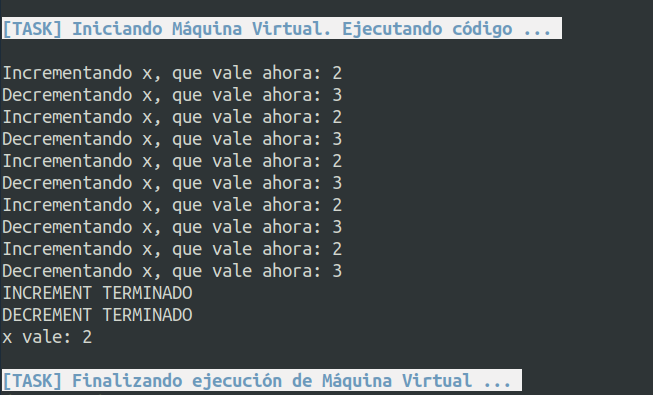
\includegraphics[width=\linewidth]{images/ejemplos/concurrentes/semaphore.png}
    \caption{Ejecución de programa: sincronización de procesos con semáforo.}
    \label{fig:lamportSemaphore_exec}
\end{figure}

En esta ejecución se observa que cada procedimiento modifica una única vez el valor de la variable global, dando como resultado final 2, que era el valor esperado tras incrementar y decrementar 1 unidad el número, el mismo número de veces.

        % Quinta parte : Conclusiones
        \part{Conclusiones}
	\chapter{\textbf{Conclusiones y trabajos futuros}}

Este proyecto ha abarcado dos áreas fundamentales relacionadas con los sistemas concurrentes y distribuidos. Primero, se llevó a cabo un estudio exhaustivo de los sistemas concurrentes, centrando la atención en una especificación formal como la propuesta por Leslie Lamport en su Lógica Temporal de Acciones (TLA). Este análisis detallado no solo proporcionó una base teórica sólida para entender la complejidad inherente a estos sistemas, sino que también destacó la importancia de una especificación rigurosa para su correcto diseño y verificación, a través del formalismo matemático.

En segundo lugar, se adoptó un enfoque práctico mediante el desarrollo de un compilador en tiempo de ejecución para un lenguaje de programación, diseñado específicamente para simular sistemas concurrentes y distribuidos. Este lenguaje se basó en el pseudocódigo utilizado en la asignatura ``Sistemas Concurrentes y Distribuidos'', permitiendo así una mayor accesibilidad y comprensión para aquellos familiarizados con el curso. La implementación de esta herramienta se realizó siguiendo una metodología de desarrollo ágil, lo que facilitó un proceso de desarrollo iterativo y adaptable.

Durante este proceso, se utilizaron herramientas avanzadas de programación, incluyendo analizadores léxicos y sintácticos, y se aprovecharon las capacidades de los lenguajes C y C++ para asegurar un rendimiento óptimo y una integración efectiva. Esta combinación de teoría y práctica no solo ha enriquecido la comprensión de los sistemas concurrentes y distribuidos, sino que también ha proporcionado una herramienta valiosa para su estudio y simulación.

Al concluir este proyecto, se ha logrado un balance entre la teoría formal y la aplicación práctica, proporcionando una perspectiva integral de los sistemas concurrentes y distribuidos. Este trabajo no solo sirve como un recurso educativo para aquellos que buscan profundizar en este campo, sino que también sienta las bases para futuras investigaciones y desarrollos en esta área tan dinámica y desafiante de la informática.

\section{Trabajos futuros}
Desarrollar un compilador completo para dar vida a un nuevo lenguaje de programación es cuanto menos desafiante, además teniendo en cuenta los cortos plazos de tiempo en los que se han desarrollado. Puesto que el software siempre está en continua evolución y en continua obsolescencia, hay algunos aspectos que se pueden mejorar y nuevas que desarrollar, citadas a continuación:

\begin{itemize}
    \item \textbf{SAAS (Software As A Service)}: Con el compilador ya dockerizado, una prometedora dirección futura para este proyecto es su desarrollo y lanzamiento como Software as a Service (SaaS). Esta transición a una plataforma basada en la nube no solo facilitaría un acceso más amplio y flexible al compilador, sino que también permitiría una gestión más eficiente y la implementación rápida de actualizaciones y mejoras. Al ofrecerlo como un servicio en la nube, podríamos expandir significativamente su alcance y utilidad, proporcionando una herramienta valiosa y accesible para una audiencia global interesada en la simulación y el estudio de sistemas concurrentes y distribuidos.
    \item \textbf{Nuevos mecanismos de sincronización y ampliación de la gramática}: De forma nativa el compilador permite definir semáforos como mecanismo de sincronización de hebras, por lo que quizá estaría bien considerar otras como ``Monitores''. También, puede considerarse ampliar la gramática de Lamport permitiendo nuevos constructos que faciliten el uso por parte del usuario.
    \item \textbf{Reimplementación de compilador en C++}: En este proyecto se utilizó C y C++ como lenguajes de desarrollo del compilador, dejando C para la parte más cercana a la fase de análisis de código (léxico, sintáctico y semántico). Aunque C es un lenguaje muy versátil a día de hoy, su sucesor C++ implementa características más seguras, en lo que concierne a gestión de memoria dinámica vía punteros. Por otra parte, su sintaxis orientada a objetos y sus múltiples bibliotecas estándar hace que la definición y/o uso de estructuras de datos sea más directa que en C, y como Flex y Bison permiten generar analizadores para este lenguaje, quizá sería conveniente reimplementar todos esos módulos con este lenguaje, garantizando más seguridad y claridad.
    \item \textbf{Gestión de errores sintácticos uniforme}: Se podría mejorar la gestión actual de los errores sintácticos por parte de Bison, definiendo unas reglas de producción más granulares y específicas, incluso teniendo en cuenta patrones incorrectos debido a tokens que no debían estar ahí.
    \item \textbf{Habilitar expresiones en definición de arrays}: Gestionar la memoria en tiempo de ejecución es una tarea ardua si las implementaciones deben hacerse desde cero, y es por eso por lo que la gramática actual, aunque contemple cualquier tipo de expresión para la declaración de arrays, se considera semánticamente incorrecta la declaración si dicha expresión no contiene exactamente un literal entero. Es por ello por lo que dentro de la memoria de la máquina virtual se podría considerar un heap que permita obtener el tamaño de los arrays en tiempo de ejecución.
    \item \textbf{Simulación realista de la asignación de los registros}: Con la estrategia actual la simulación que hace la máquina virtual es menos realista que lo que se hace en una máquina convencional. Se podría considerar cambiar esta mecánica de decisión de registros a la hora de generar las instrucciones de la representación intermedia, comprobando la vivacidad de los registros.
\end{itemize}

Para concluir, este proyecto no solo representa un paso significativo en la simulación y estudio de sistemas concurrentes y distribuidos, sino que también establece una sólida base para futuras innovaciones y mejoras. Con estas vías futuras, el proyecto está bien posicionado para adaptarse y evolucionar, manteniéndose relevante y útil en un campo que está en constante cambio y crecimiento.


	
	\newpage
        \nocite{*}
	\bibliography{bibliografia}
	\bibliographystyle{plain}
	
\end{document}

